\documentclass[a4paper,10pt]{book}

\usepackage{eulervm}

% packages
\usepackage[utf8]{inputenc}
\usepackage{xcolor,colortbl}
\usepackage{makecell}
\usepackage{booktabs}
\usepackage{amsthm}
\usepackage{amsfonts}
\usepackage{amsmath}
\usepackage{tikz}
\usepackage{graphicx}
\usepackage{amssymb}
\usepackage[]{algorithm}
\usepackage[noend]{algorithmic}
\usepackage{enumerate}% http://ctan.org/pkg/enumerate
\usepackage{varwidth}

\usepackage{url}
\usepackage{cite}
\usepackage{tikz}
\usepackage{amsmath,amssymb,amsfonts}
\usepackage[]{algorithm}
\usepackage[noend]{algorithmic}
\usepackage{graphicx}
\usepackage{textcomp}
\usepackage{amsthm}
\usepackage{xstring}
\usepackage{tabstackengine}
\usepackage[space]{grffile}
\usepackage{subfig}
\usepackage{balance}

\usepackage{tabularx}



%%
%\algnewcommand{\LineComment}[1]{\State \(\triangleright\) #1}
%% colors
\definecolor{green}{RGB}{169,223,191}
\definecolor{darkgreen}{RGB}{46,139,87}
\definecolor{gray}{RGB}{160,160,160}
\definecolor{lightgray}{RGB}{220,220,220}
\definecolor{darkgray}{RGB}{120,120,120}
\definecolor{seagreen}{RGB}{46,139,87}

\definecolor{router}{RGB}{255,255,255}
\definecolor{marked}{RGB}{220,220,220}

\usetikzlibrary{calc}

%

% theorems
\newtheorem{theorem}{Theorem}[chapter]
\newtheorem{proposition}[theorem]{Proposition}
\newtheorem{lemma}[theorem]{Lemma}
\newtheorem{corollary}[theorem]{Corollary}
\newtheorem{definition}{Definition}[chapter]
\newtheorem*{observation*}{Observation}
\newcommand{\just}[1]{\tag*{\footnotesize {\color{darkgray}[#1]}}}

%%

% notations
\newcommand{\fset}{F}
\newcommand{\powerset}{\mathcal{P}}
\newcommand{\igp}{\mathsf{igp}}
\newcommand{\lat}{\mathsf{lat}}
\newcommand{\bnd}{\mathsf{cap}}
\newcommand{\idx}{\mathsf{idx}}

\newcommand{\src}{\mathit{src}}
\newcommand{\dst}{\mathit{dst}}
\newcommand{\vol}{\mathit{vol}}


\newcommand{\mcflp}{\textsf{MCF-LP}}
\newcommand{\srtepath}{\textsf{SRTE-PATH}}
\newcommand{\srtepathdem}{\textsf{SRTE-DEM}}
\newcommand{\srtepathlp}{\textsf{SRTE-DEM-LP}}
\newcommand{\srtepathlpdual}{\textsf{SRTE-DEM-DUAL}}
\newcommand{\bhatia}{\textsf{SRTE-1DET}}
\newcommand{\srteseg}{\textsf{SRTE-SEG}}
\newcommand{\PB}{P_1}


\renewcommand{\sp}{\mathsf{SP}}
\newcommand{\SP}{\mathsf{SP}}
\newcommand{\seq}{\mathsf{path}}

\newcommand{\oute}{\delta^+}
\newcommand{\ine}{\delta^-}
\newcommand{\outn}{\mathcal{N}^+}
\newcommand{\inn}{\mathcal{N}^-}

\newcommand{\dist}{d}


\newcommand{\latmax}{\mathit{lat}_\mathit{M}}
\newcommand{\latavg}{\mathit{lat}_\mu}

\newcommand{\adj}{\textsf{adj}}

\newcommand{\cnt}{\mathcal{C}}

%%

\newcommand{\algrule}[1][.2pt]{\par\vskip.5\baselineskip\hrule height #1\par\vskip.5\baselineskip}

\newcommand{\Pk}{\mathcal{\sr{P}}_k}
\newcommand{\Csk}{\mathcal{\sr{C}}^s_k}

% sr
\newcommand{\sr}[1]{\vec{#1}}
\newcommand{\len}{\textit{len}}
\newcommand{\seg}{\textit{seg}}

\newcommand{\nreach}{\textsf{reach}}
\newcommand{\ereach}{\textsf{e-reach}}

\newcommand{\spreach}{\textsf{sp-reach}}

\newcommand{\kn}{k_n}
\newcommand{\ke}{k_e}

\newcommand{\kM}{k_{\max}}
\newcommand{\km}{k_{\min}}

\renewcommand{\r}{\tau}
\newcommand{\load}{\mathsf{load}}
\newcommand{\rev}{\mathsf{rev}}


\newcommand{\name}{CG4SR}  % Temporary name

\newcommand{\node}{\textit{node}}

\newcommand{\cost}{\textsf{sr-cost}}
\newcommand{\mseg}{\textsf{min-seg}}
\newcommand{\NPhard}{\textsf{NP-hard}}
\newcommand{\NPcomplete}{\textsf{NP-complete}}
\renewcommand{\node}[1]{\texttt{#1}}
\newcommand{\topo}[1]{\textsf{#1}}

\renewcommand{\P}[1]{\mathcal{P}}
\newcommand{\D}[1]{\mathcal{D}}


\newcommand{\edge}[2]{(\node{#1}, \node{#2})}


%%% CG CYCLE COVER

\newcommand{\ccPrimalMip}{\textsf{SRCC}}
\newcommand{\ccPrimalLp}{\textsf{SRCC-LP}}
\newcommand{\ccDualLp}{\textsf{SRCC-DUAL}}

\newcommand{\ccPrimalLpK}{\textsf{SRCC-LP-K}}
\newcommand{\ccDualLpK}{\textsf{SRCC-DUAL-K}}


%%

% tikz
\usetikzlibrary{calc, shadings, shadows, shapes.arrows}
\usetikzlibrary{positioning,arrows,backgrounds,decorations.pathmorphing}

\tikzset{%
  interface/.style={draw, rectangle, rounded corners, font=\LARGE\sffamily},
  ethernet/.style={interface, fill=yellow!50},% ethernet interface
  serial/.style={interface, fill=green!70},% serial interface
  speed/.style={sloped, anchor=south, font=\large\sffamily},% line speed at edge
  route/.style={draw, shape=single arrow, single arrow head extend=4mm,
    minimum height=1.7cm, minimum width=3mm,
    drop shadow={opacity=0, fill=black}, font=\tiny}% inroute / outroute arrows
}
\newcommand*{\shift}{1.3cm}
\newcommand*{\router}[2]{
\begin{tikzpicture}[yscale=1.5]   
  \coordinate (ll) at (-3,0.5);
  \coordinate (lr) at (3,0.5);
  \coordinate (ul) at (-3,2);
  \coordinate (ur) at (3,2);
  \draw [line width=2, fill=#2] (ll) arc (-180:0:3cm and .75cm) -- (ur) arc (0:-180:3cm and .75cm)
    -- cycle;
  \draw [line width=2, fill=#2] (ul)
    arc (-180:180:3cm and .75cm);
  \node[text width=5cm,text centered,font=\bfseries] at (0,0.5){};
  \node[scale=5,text centered,font=\bfseries] at (0,0.5){#1};
  
  \begin{scope}[yshift=2cm, yscale=0.28, transform shape]
    \node[very thick, route, rotate=45, xshift=\shift] {\strut};
    \node[very thick, route, rotate=-45, xshift=-\shift] {\strut};
    \node[very thick, route, rotate=-135, xshift=\shift] {\strut};
    \node[very thick, route, rotate=135, xshift=-\shift] {\strut};
  \end{scope}
\end{tikzpicture}}

\tikzset{
  wavy/.style = {
     decorate,
     decoration = {snake, amplitude=1.5mm, segment length=8mm}
  },
  main node/.style={circle,fill=gray!25,draw,font=\sffamily\Large\bfseries}
}
%%
\newcommand{\lnt}[1]{\overline{\ln}^{#1}}

\newcommand{\todo}[1]{{\color{red}\textbf{TODO:~}#1}}
\newcommand{\note}[1]{{\color{orange}#1}}

\newcommand{\question}[1]{{\color{cyan}#1}}


\newcommand{\crit}{\mathsf{cr}}

\newcommand{\forw}{\mathsf{forw}}
\newcommand{\fail}{\mathsf{fail}}

\newcommand{\maxflow}{\textsf{MAX-FLOW}}
\newcommand{\maxedp}{\textsf{MAX-EDP}}
\newcommand{\minlatedp}{\textsf{MIN-LAT-EDP}}
\newcommand{\sredpseg}{\textsf{SR-EDP-SEG}}
\newcommand{\sredpfortz}{\textsf{SR-EDP-FORTZ}}
\newcommand{\sredp}{\textsf{SR-2EDP}}

\newcommand{\hide}[1]{{\color{gray} #1}}

\newcommand{\cmt}[1]{{\color{darkgreen}$\quad$[#1]}}
\newcommand{\cmtline}[1]{\STATE {\color{darkgreen}[#1]}}

\newcounter{pbcnt}[chapter]
\newenvironment{problem}[1]% environment name
{
  \refstepcounter{pbcnt}
  \setlength{\parindent}{0pt}
  \par\vspace{\baselineskip}
  \textbf{Problem \thepbcnt~(#1)}\begin{itshape}%
  \par\vspace{\baselineskip}\ignorespaces
}
{
  \end{itshape}\ignorespacesafterend\newline
} 

\begin{document}

\tableofcontents

%\todo{have a section explaining how to read CDF}
\chapter{Introduction}
\label{chapter:into}

This thesis aims at providing a first mathematical formalization of segment routing and 
showcase several of its use cases. We believe that such a formalization is
going to help advance the research of the algorithmic aspects of segment routing by
providing a solid mathematical foundation and notations which can serve as a starting
point for others to research this topic.
The presented use cases validate the practical interest of the deployment of segment routing
on existing networks.

Traditional networks use shortest path routing to forward the packets between the routers
in the network. Without going into details of shortest path routing, each link in the network 
has a weight configured on it and shortest paths are computed with respect to these weights. We refer to these weights
as interior gateway protocol weights (IGP weights). These paths are
used to create a routing table on each router that maps the destination of the packet to an outgoing link interface.
In this way, when a packet to $dst$ reaches a router, that router will inspect its routing table to find out
the link interface towards which it needs to forward that packet. By doing so, the packet will reach $dst$ by traversing the
shortest path relative to these IGP weights. 
Figure \ref{fig:intro_sprouting} provides a high level illustration of shortest path routing of the Abilene network \cite{abilene}.
When forwarding packets from router \node{a} to \node{i}, the shortest path, shown in green, will be traversed.
The table on top of router \node{d} shows an abstraction of its routing
table. When \node{d} receives a packet with destination \node{i}, it inspects its routing table and sees that
the next hop in the IGP shortest path to \node{i} is \node{e} so it forwards it there.
All of this is an abstraction of what really goes on in a real network because it hides a lot of technical 
aspects like, for instance, the fact that the information stored is the IP address. However, for this thesis, this view is accurate enough as we focus on mathematical optimization problems related to
computer networks rather than compute networks per se.

\begin{figure}[H]
\begin{center}
\begin{tikzpicture}
\def\x{0}
\def\y{0}
\node[scale=0.15] (a) at (0 + \x,  0 + \y) {\router{a}{green}};
\node[scale=0.15] (b) at (-1 + \x,  -2 + \y) {\router{b}{router}};
\node[scale=0.15] (c) at (0 + \x,  -3.5 + \y) {\router{c}{router}};
\node[scale=0.15] (d) at (2.5 + \x,  -1.5 + \y) {\router{d}{router}};
\node[scale=0.15] (e) at (4.5 + \x,  -2 + \y) {\router{e}{router}};
\node[scale=0.15] (f) at (4 + \x,  -4 + \y) {\router{f}{router}};
\node[scale=0.15] (i) at (7 + \x,  -3.5 + \y) {\router{i}{green}};
\node[scale=0.15] (h) at (7 + \x,  -1.8 + \y) {\router{h}{router}};
\node[scale=0.15] (g) at (5.8 + \x,  -0.5 + \y) {\router{g}{router}};
\node[scale=0.15] (k) at (9.5 + \x,  -2 + \y) {\router{k}{router}};
\node[scale=0.15] (j) at (10 + \x,  0 + \y) {\router{j}{router}};
\draw[line width=2] (a) edge[above, sloped] node[black,font=\bfseries] {\footnotesize \texttt{42}} (b);
\draw[line width=2] (b) edge[below, sloped] node[black,font=\bfseries] {\footnotesize \texttt{46}} (c);
\draw[line width=2] (b) edge[below, sloped] node[black,font=\bfseries] {\footnotesize \texttt{34}} (d);
\draw[line width=2] (a) edge[below, sloped] node[black,font=\bfseries] {\footnotesize \texttt{31}} (d);
\draw[line width=2] (c) edge[below, sloped] node[black,font=\bfseries] {\footnotesize \texttt{35}} (f);
\draw[line width=2] (d) edge[below, sloped] node[black,font=\bfseries] {\footnotesize \texttt{43}} (e);
\draw[line width=2] (e) edge[above, sloped] node[black,font=\bfseries] {\footnotesize \texttt{27}} (f);
\draw[line width=2] (e) edge[above, sloped] node[black,font=\bfseries] {\footnotesize \texttt{21}} (g);
\draw[line width=2] (g) edge[above, sloped] node[black,font=\bfseries] {\footnotesize \texttt{11}} (h);
\draw[line width=2] (h) edge[below, sloped] node[black,font=\bfseries] {\footnotesize \texttt{27}} (i);
\draw[line width=2] (f) edge[below, sloped] node[black,font=\bfseries] {\footnotesize \texttt{30}} (i);
\draw[line width=2] (g) edge[above, sloped] node[black,font=\bfseries] {\footnotesize \texttt{61}} (j);
\draw[line width=2] (j) edge[above, sloped] node[black,font=\bfseries] {\footnotesize \texttt{52}} (k);
\draw[line width=2] (k) edge[above, sloped] node[black,font=\bfseries] {\footnotesize \texttt{42}} (i);
\draw[line width=3, darkgreen] (a) edge[->] (d);
\draw[line width=3, darkgreen] (d) edge[->] (e);
\draw[line width=3, darkgreen] (e) edge[->] (f);
\draw[line width=3, darkgreen] (f) edge[->] (i);
%\draw[darkgreen, line width=3, ->] plot [smooth] coordinates { ($(a)+(0.6,0.1)$) ($(d)+(0,0.5)$) ($(e)+(0,0.6)$) ($(e)+(0.6,0)$) ($(f)+(0.5,0.5)$) ($(i)+(-0.5,0.25)$) };


\node (t) at (\x + 3.5, \y + 1) {
\begin{tabular}{|c|c|}
\hline
dest & next hop \\
\hline
$\vdots$ & $\vdots$ \\
\hline
\node{c} & \node{b} \\
\hline
\rowcolor{green}
\node{i} & \node{e} \\
\hline
\node{j} & \node{e} \\
\hline
$\vdots$ & $\vdots$ \\
\hline
\end{tabular}
};

\draw[line width=1, dotted] (d) -- (t);
\end{tikzpicture}
\end{center}
\caption{Illustration of shortest path routing on the Abilene network.}
\label{fig:intro_sprouting}
\end{figure}

During recent years, networking vendors and network operators have
designed \cite{filsfils2015segment,rfc8402}, implemented
\cite{srdemo} and deployed \cite{schuller2017traffic,srdeploy} 
a new routing architecture called Segment Routing (SR). Segment
Routing is a modern variant of source routing which can be used in
either MPLS or IPv6 networks. In a nutshell, Segment Routing allows
the source of a packet or the ingress node in a network to easily
specify the path that packets need to follow inside the
network. This path is specified as a series of labels, called \emph{segments}, (MPLS labels or
IPv6 addresses in a special IPv6 header extension) that are added to
each packet. These segment are stored as a stack and are popped out as the packets reaches
the routers or links they represent. Some implementations do not explicitly remove the segments
but rather keep a point to the next segment.

More concretely, a segment routing path is composed of one or more segments. 
There are two types of segments: $(i)$ \emph{node} and $(ii)$ \emph{adjacency} segments. 
Node segments represent routers. When a node segment is at the top of the stack, the packet is routed towards the corresponding router using
standard shortest path routing. Figure \ref{fig:srnode} shows an example over the Abilene network of what happens when packets are
sent from \node{a} to \node{i} using segment routing with one intermediate node segment representing node \node{g}. First, \node{a} will inspect the
segment stack and see a node segment representing router \node{g}. It will pop this segment and forward the packet using
shortest path routing to \node{g}. Then, node \node{g} will inspect the packet header and see that the next segment is router \node{i}.
It will pop this segment and forward the packet using shortest path routing to \node{i}. At this point the segment stack is empty so the
packet as arrived to its destination.

\begin{figure}[H]
\begin{center}
\begin{tikzpicture}
\def\x{0}
\def\y{0}
\node[scale=0.15] (a) at (0 + \x,  0 + \y) {\router{a}{green}};
\node[scale=0.15] (b) at (-1 + \x,  -2 + \y) {\router{b}{router}};
\node[scale=0.15] (c) at (0 + \x,  -3.5 + \y) {\router{c}{router}};
\node[scale=0.15] (d) at (2.5 + \x,  -1.5 + \y) {\router{d}{router}};
\node[scale=0.15] (e) at (4.5 + \x,  -2 + \y) {\router{e}{router}};
\node[scale=0.15] (f) at (4 + \x,  -4 + \y) {\router{f}{router}};
\node[scale=0.15] (i) at (7 + \x,  -3.5 + \y) {\router{i}{green}};
\node[scale=0.15] (h) at (7 + \x,  -1.8 + \y) {\router{h}{router}};
\node[scale=0.15] (g) at (5.8 + \x,  -0.5 + \y) {\router{g}{green}};
\node[scale=0.15] (k) at (9.5 + \x,  -2 + \y) {\router{k}{router}};
\node[scale=0.15] (j) at (10 + \x,  0 + \y) {\router{j}{router}};
\draw[line width=2] (a) edge[above, sloped] node[black,font=\bfseries] {\footnotesize \texttt{42}} (b);
\draw[line width=2] (b) edge[below, sloped] node[black,font=\bfseries] {\footnotesize \texttt{46}} (c);
\draw[line width=2] (b) edge[below, sloped] node[black,font=\bfseries] {\footnotesize \texttt{34}} (d);
\draw[line width=2] (a) edge[below, sloped] node[black,font=\bfseries] {\footnotesize \texttt{31}} (d);
\draw[line width=2] (c) edge[below, sloped] node[black,font=\bfseries] {\footnotesize \texttt{35}} (f);
\draw[line width=2] (d) edge[below, sloped] node[black,font=\bfseries] {\footnotesize \texttt{43}} (e);
\draw[line width=2] (e) edge[below, sloped] node[black,font=\bfseries] {\footnotesize \texttt{27}} (f);
\draw[line width=2] (e) edge[above, sloped] node[black,font=\bfseries] {\footnotesize \texttt{21}} (g);
\draw[line width=2] (g) edge[above, sloped] node[black,font=\bfseries] {\footnotesize \texttt{11}} (h);
\draw[line width=2] (h) edge[above, sloped] node[black,font=\bfseries] {\footnotesize \texttt{27}} (i);
\draw[line width=2] (f) edge[above, sloped] node[black,font=\bfseries] {\footnotesize \texttt{35}} (i);
\draw[line width=2] (g) edge[above, sloped] node[black,font=\bfseries] {\footnotesize \texttt{61}} (j);
\draw[line width=2] (j) edge[above, sloped] node[black,font=\bfseries] {\footnotesize \texttt{52}} (k);
\draw[line width=2] (k) edge[above, sloped] node[black,font=\bfseries] {\footnotesize \texttt{42}} (i);
\draw[line width=3, darkgreen] (a) edge[->] (d);
\draw[line width=3, darkgreen] (d) edge[->] (e);
\draw[line width=3, darkgreen] (e) edge[->] (g);

\draw[line width=3, darkgreen] (g) edge[->] (h);
\draw[line width=3, darkgreen] (h) edge[->] (i);

\node[above of=a] (s1) {
\begin{tabular}{|c|c|}
\hline
\node{g} & \node{i} \\
\hline
\end{tabular}
};

\draw[line width=1, dotted] (a) -- (s1);

\node[above of=g] (s2) {
\begin{tabular}{|c|}
\hline
\node{i} \\
\hline
\end{tabular}
};

\draw[line width=1, dotted] (g) -- (s2);
\end{tikzpicture}
\end{center}
\caption{Illustration of SR from \node{a} to \node{i} with a node segment on \node{g}.}
\label{fig:srnode}
\end{figure}

Adjacency segments represent links. When an adjacency segment is at the top of the stack, the packet is routed towards the origin of the edge
corresponding to the link using standard shortest path routing. Then, it is forwarded over that specific link to the router corresponding
to the destination of that edge.

Figure \ref{fig:sradj} illustrates an example of what happens when packets are
sent from \node{a} to \node{i} using segment routing with an adjacency segment representing edge $(\node{g}, \node{j})$. First, \node{a} will inspect the
segment stack and see an adjacency segment representing edge $(\node{g}, \node{j})$. It will forward the packet using
shortest path routing to \node{g}. Then, node \node{g} will inspect the packet header and see that there is an adjacency segment of which he is the origin.
It pops the adjacency segment from the segment stack and sends it over edge $(\node{g}, \node{j})$. From there,
\node{j} will inspect the segment stack and see that in needs to forward that packet towards \node{i}.

\begin{figure}[H]
\begin{center}
\begin{tikzpicture}
\def\x{0}
\def\y{0}
\node[scale=0.15] (a) at (0 + \x,  0 + \y) {\router{a}{green}};
\node[scale=0.15] (b) at (-1 + \x,  -2 + \y) {\router{b}{router}};
\node[scale=0.15] (c) at (0 + \x,  -3.5 + \y) {\router{c}{router}};
\node[scale=0.15] (d) at (2.5 + \x,  -1.5 + \y) {\router{d}{router}};
\node[scale=0.15] (e) at (4.5 + \x,  -2 + \y) {\router{e}{router}};
\node[scale=0.15] (f) at (4 + \x,  -4 + \y) {\router{f}{router}};
\node[scale=0.15] (i) at (7 + \x,  -3.5 + \y) {\router{i}{green}};
\node[scale=0.15] (h) at (7 + \x,  -1.8 + \y) {\router{h}{router}};
\node[scale=0.15] (g) at (5.8 + \x,  -0.5 + \y) {\router{g}{green}};
\node[scale=0.15] (k) at (9.5 + \x,  -2 + \y) {\router{k}{router}};
\node[scale=0.15] (j) at (10 + \x,  0 + \y) {\router{j}{green}};
\draw[line width=2] (a) edge[above, sloped] node[black,font=\bfseries] {\footnotesize \texttt{42}} (b);
\draw[line width=2] (b) edge[below, sloped] node[black,font=\bfseries] {\footnotesize \texttt{46}} (c);
\draw[line width=2] (b) edge[below, sloped] node[black,font=\bfseries] {\footnotesize \texttt{34}} (d);
\draw[line width=2] (a) edge[below, sloped] node[black,font=\bfseries] {\footnotesize \texttt{31}} (d);
\draw[line width=2] (c) edge[below, sloped] node[black,font=\bfseries] {\footnotesize \texttt{35}} (f);
\draw[line width=2] (d) edge[below, sloped] node[black,font=\bfseries] {\footnotesize \texttt{43}} (e);
\draw[line width=2] (e) edge[below, sloped] node[black,font=\bfseries] {\footnotesize \texttt{27}} (f);
\draw[line width=2] (e) edge[above, sloped] node[black,font=\bfseries] {\footnotesize \texttt{21}} (g);
\draw[line width=2] (g) edge[above, sloped] node[black,font=\bfseries] {\footnotesize \texttt{11}} (h);
\draw[line width=2] (h) edge[above, sloped] node[black,font=\bfseries] {\footnotesize \texttt{27}} (i);
\draw[line width=2] (f) edge[above, sloped] node[black,font=\bfseries] {\footnotesize \texttt{35}} (i);
\draw[line width=2] (g) edge[above, sloped] node[black,font=\bfseries] {\footnotesize \texttt{61}} (j);
\draw[line width=2] (j) edge[above, sloped] node[black,font=\bfseries] {\footnotesize \texttt{52}} (k);
\draw[line width=2] (k) edge[above, sloped] node[black,font=\bfseries] {\footnotesize \texttt{42}} (i);
\draw[line width=3, darkgreen] (a) edge[->] (d);
\draw[line width=3, darkgreen] (d) edge[->] (e);
\draw[line width=3, darkgreen] (e) edge[->] (g);
\draw[line width=4, dotted, darkgreen] (g) edge[->] (j);

\draw[line width=3, darkgreen] (j) edge[->] (k);
\draw[line width=3, darkgreen] (k) edge[->] (i);

\node[above of=a] (s1) {
\begin{tabular}{|c|c|}
\hline
$(\node{g}, \node{j})$ & \node{i} \\
\hline
\end{tabular}
};

\draw[line width=1, dotted] (a) -- (s1);

\node[above of=g] (s2) {
\begin{tabular}{|c|c|}
\hline
$(\node{g}, \node{j})$ & \node{i} \\
\hline
\end{tabular}
};


\node[above of=j] (s3) {
\begin{tabular}{|c|}
\hline
\node{i} \\
\hline
\end{tabular}
};

\draw[line width=1, dotted] (g) -- (s2);
\end{tikzpicture}
\end{center}
\caption{Illustration of SR from \node{a} to \node{i} with an adjacency segment on $(\node{g}, \node{j})$.}
\label{fig:sradj}
\end{figure}

\section{Why segment routing}

Segments routing offers a lot of flexibility for routing packets by allowing to exploit non shortest path as illustrated
in Figures \ref{fig:srnode} and \ref{fig:sradj}.
It does so by leveraging traditional IP routing so it is easily implementable on current networks without
needing to change the way networks operate or their infrastructure. Moreover, there is no need for routers
to maintain more state than their, already existing, routing tables. The only overhead is on the packet header
which now needs to contain the segment stack.

SR is not the first technique to have been developed that makes it possible to route over non shortest paths. 
Another technique is to use Multiprotocol Label Switching (MPLS) \cite{Ghein:2006:MF:1206881}. In a high level, MPLS works by
configuring label forwarding tables on the routers. Conceptually, these tables are similar to the routing tables except that
they are not built with respect to the IGP weights. Instead, they map pairs of (label, incoming interface) into other pairs (label, outgoing interface). 
Figure \ref{fig:mpls} shows an example of how a MPLS configuration can allow us to route packets from
\node{a} to \node{c} over the non-shortest path $(\node{a}, \node{d}, \node{b}, \node{c})$. In this example, this is achieved by configuring the labeling table of \node{d} to map 
packets coming from the interface corresponding to link $(\node{a}, \node{d})$ with label $5$ to label $8$
and link $(\node{d}, \node{b})$. Second, we configure the labeling
table of \node{b} to map packets coming from link $(\node{d}, \node{b})$ with label $8$ to be routed over $(\node{b}, \node{c})$
with the same label.

\begin{figure}[H]
\begin{center}
\begin{tikzpicture}
\def\x{0}
\def\y{0}
\node[scale=0.15] (a) at (0 + \x,  0 + \y) {\router{a}{green}};
\node[scale=0.15] (b) at (-1 + \x,  -2 + \y) {\router{b}{green}};
\node[scale=0.15] (c) at (0 + \x,  -3.5 + \y) {\router{c}{router}};
\node[scale=0.15] (d) at (2.5 + \x,  -1.5 + \y) {\router{d}{router}};
\node[scale=0.15] (e) at (4.5 + \x,  -2 + \y) {\router{e}{router}};
\node[scale=0.15] (f) at (4 + \x,  -4 + \y) {\router{f}{router}};
\node[scale=0.15] (i) at (7 + \x,  -3.5 + \y) {\router{i}{router}};
\node[scale=0.15] (h) at (7 + \x,  -1.8 + \y) {\router{h}{router}};
\node[scale=0.15] (g) at (5.8 + \x,  -0.5 + \y) {\router{g}{router}};
\node[scale=0.15] (k) at (9.5 + \x,  -2 + \y) {\router{k}{router}};
\node[scale=0.15] (j) at (10 + \x,  0 + \y) {\router{j}{router}};
\draw[line width=2] (a) edge[above, sloped] node[black,font=\bfseries] {\footnotesize \texttt{42}} (b);
\draw[line width=2] (b) edge[below, sloped] node[black,font=\bfseries] {\footnotesize \texttt{46}} (c);
\draw[line width=2] (b) edge[below, sloped] node[black,font=\bfseries] {\footnotesize \texttt{34}} (d);
\draw[line width=2] (a) edge[below, sloped] node[black,font=\bfseries] {\footnotesize \texttt{31}} (d);
\draw[line width=2] (c) edge[below, sloped] node[black,font=\bfseries] {\footnotesize \texttt{35}} (f);
\draw[line width=2] (d) edge[below, sloped] node[black,font=\bfseries] {\footnotesize \texttt{43}} (e);
\draw[line width=2] (e) edge[below, sloped] node[black,font=\bfseries] {\footnotesize \texttt{27}} (f);
\draw[line width=2] (e) edge[above, sloped] node[black,font=\bfseries] {\footnotesize \texttt{21}} (g);
\draw[line width=2] (g) edge[above, sloped] node[black,font=\bfseries] {\footnotesize \texttt{11}} (h);
\draw[line width=2] (h) edge[above, sloped] node[black,font=\bfseries] {\footnotesize \texttt{27}} (i);
\draw[line width=2] (f) edge[above, sloped] node[black,font=\bfseries] {\footnotesize \texttt{35}} (i);
\draw[line width=2] (g) edge[above, sloped] node[black,font=\bfseries] {\footnotesize \texttt{61}} (j);
\draw[line width=2] (j) edge[above, sloped] node[black,font=\bfseries] {\footnotesize \texttt{52}} (k);
\draw[line width=2] (k) edge[above, sloped] node[black,font=\bfseries] {\footnotesize \texttt{42}} (i);

\draw[line width=3, darkgreen] (a) edge[->] (d);
\draw[line width=3, darkgreen] (d) edge[->] (b);
\draw[line width=3, darkgreen] (b) edge[->] (c);


\node (p1) at (\x + 2, \y + -0.25) {
\begin{tabular}{|c|c|}
\hline
\footnotesize 5 & \footnotesize data \\
\hline
\end{tabular}
};

\draw[line width=1, dashed] (p1) -- (1.5, -0.8);


\node (p2) at (\x + 2.5, \y + -2.3) {
\begin{tabular}{|c|c|}
\hline
\footnotesize 8 & \footnotesize data \\
\hline
\end{tabular}
};

\draw[line width=1, dashed] (p2) -- (1.5, -1.8);


\node (t) at (\x + 5, \y + 1.5) {
\begin{tabular}{|c|c|c|c|}
\hline
lbl in & in inter & lbl out & out inter \\
\hline
$\vdots$ & $\vdots$ & $\vdots$ & $\vdots$ \\
\hline
\rowcolor{green}
5 & (\node{a}, \node{d}) & 8 & (\node{d}, \node{b}) \\
\hline
$\vdots$ & $\vdots$ & $\vdots$ & $\vdots$ \\
\hline
\end{tabular}
};

\draw[line width=1, dotted] (d) -- (t);

\node (t2) at (\x + 2, \y + -6) {
\begin{tabular}{|c|c|c|c|}
\hline
lbl in & in inter & lbl out & out inter \\
\hline
$\vdots$ & $\vdots$ & $\vdots$ & $\vdots$ \\
\hline
\rowcolor{green}
8 & (\node{d}, \node{b}) & 8 & (\node{b}, \node{c}) \\
\hline
$\vdots$ & $\vdots$ & $\vdots$ & $\vdots$ \\
\hline
\end{tabular}
};

\draw[line width=1, dotted] (b) -- (-0.75, -4.8);

\node (p3) at (\x + 1.5, \y + -2.3-0.75) {
\begin{tabular}{|c|c|}
\hline
\footnotesize 8 & \footnotesize data \\
\hline
\end{tabular}
};

\draw[line width=1, dashed] (p3) -- (-0.5, -2.5);

\end{tikzpicture}
\end{center}
\caption{Illustration of MPLS.}
\label{fig:mpls}
\end{figure}

One drawback of MPLS when compared to segment routing is that the routers need to maintain an extra state,
namely, the labeling tables. This makes it harder for solutions based on MPLS to scale has these
labeling tables can become huge if a lot of different paths are configured~\cite{rfc5439,defo-sig15}. 
MPLS also has some operational limitations \cite{mpls-opissues-ripe64} and makes a sub-optimal usage
of resources~\cite{mpls-latency-imc11}.

In contrast, as we mentioned above, with segment
routing only the ingress node needs to maintain a state and all the path information is inserted in 
the packed header as segment. However, one drawback of SR is that, due to hardware limitations, some commercial routers only support a very limited amount
of segments \cite{Tantsura_SID:2017}. An average low end router can support up to 5 segments whereas high end router can go up to 
about 10 segments.

Other more recent techniques exist that overcome these limitations as, for instance, Fibbing \cite{Vissicchio:2014:SLL:2670518.2673868}.
Fibbing is an new architecture proposed in  2014 that enables central control over distributed routing. By doing so, similarly to segment routing, it 
combines the advantages of software defined networks (flexibility, expressiveness, and manageability) and traditional approaches (robustness, and scalability).

The way Fibbing works is that it introduces fake nodes and links into an underlying link-state routing protocol. The fake routers and links
are then taken into account by routers when computing their forwarding tables. Figure \ref{fig:intro_fibbing} illustrates how to implement
the non shortest path $(\node{a}, \node{d}, \node{b}, \node{c})$ with fibbing. To do so, we can introduce a fake node \node{x} connected to \node{a} and \node{d}.
This fake node advertises that it can reach \node{c} directly, with a weight of 1. Therefore, from the point of view of \node{a}, the next hop
on the shortest path to \node{c} is not \node{b} but rather \node{x}. We ensure that the table are configured in a way such that when \node{a}
sends packets towards fake node \node{x}, link $(\node{a}, \node{d})$ is used. In this way, \node{a} will send the packets to \node{d}
and then from there routing will be done normally using shortest path $(\node{d}, \node{b}, \node{c})$. 


\begin{figure}[H]
\begin{center}
\begin{tikzpicture}
\def\x{0}
\def\y{0}
\node[scale=0.15] (a) at (0 + \x,  0 + \y) {\router{a}{green}};
\node[scale=0.15] (b) at (-1 + \x,  -2 + \y) {\router{b}{router}};
\node[scale=0.15] (c) at (0 + \x,  -3.5 + \y) {\router{c}{router}};
\node[scale=0.15] (d) at (2.5 + \x,  -1.5 + \y) {\router{d}{router}};
\node[scale=0.15] (e) at (4.5 + \x,  -2 + \y) {\router{e}{router}};
\node[scale=0.15] (f) at (4 + \x,  -4 + \y) {\router{f}{router}};
\node[scale=0.15] (i) at (7 + \x,  -3.5 + \y) {\router{i}{router}};
\node[scale=0.15] (h) at (7 + \x,  -1.8 + \y) {\router{h}{router}};
\node[scale=0.15] (g) at (5.8 + \x,  -0.5 + \y) {\router{g}{router}};
\node[scale=0.15] (k) at (9.5 + \x,  -2 + \y) {\router{k}{router}};
\node[scale=0.15] (j) at (10 + \x,  0 + \y) {\router{j}{router}};

\node[draw, fill=marked] (x) at (0.5 + \x,  -1 + \y) {\footnotesize \texttt{x}};

\draw[line width=2] (a) edge[below, sloped] node[black,font=\bfseries] {\footnotesize \texttt{1}} (x);

\draw[line width=2] (a) edge[above, sloped] node[black,font=\bfseries] {\footnotesize \texttt{42}} (b);
\draw[line width=2] (b) edge[below, sloped] node[black,font=\bfseries] {\footnotesize \texttt{46}} (c);
\draw[line width=2] (b) edge[below, sloped] node[black,font=\bfseries] {\footnotesize \texttt{34}} (d);
\draw[line width=2] (a) edge[above, sloped] node[black,font=\bfseries] {\footnotesize \texttt{31}} (d);
\draw[line width=2] (c) edge[below, sloped] node[black,font=\bfseries] {\footnotesize \texttt{35}} (f);
\draw[line width=2] (d) edge[below, sloped] node[black,font=\bfseries] {\footnotesize \texttt{43}} (e);
\draw[line width=2] (e) edge[above, sloped] node[black,font=\bfseries] {\footnotesize \texttt{27}} (f);
\draw[line width=2] (e) edge[above, sloped] node[black,font=\bfseries] {\footnotesize \texttt{21}} (g);
\draw[line width=2] (g) edge[above, sloped] node[black,font=\bfseries] {\footnotesize \texttt{11}} (h);
\draw[line width=2] (h) edge[below, sloped] node[black,font=\bfseries] {\footnotesize \texttt{27}} (i);
\draw[line width=2] (f) edge[below, sloped] node[black,font=\bfseries] {\footnotesize \texttt{30}} (i);
\draw[line width=2] (g) edge[above, sloped] node[black,font=\bfseries] {\footnotesize \texttt{61}} (j);
\draw[line width=2] (j) edge[above, sloped] node[black,font=\bfseries] {\footnotesize \texttt{52}} (k);
\draw[line width=2] (k) edge[above, sloped] node[black,font=\bfseries] {\footnotesize \texttt{42}} (i);


\draw[darkgreen, line width=3, ->] plot [smooth] coordinates { ($(a)+(0.3,-0.3)$) ($(x)+(0,0.3)$) ($(1.25, -0.75)$) ($(d)+(-0.5,0.2)$) };

\draw[line width=2, dotted] (x) edge[above, sloped] node {\footnotesize \texttt{1}} (c);

%\draw[line width=3, darkgreen] (a) edge[->] (d);
\draw[line width=3, darkgreen] (d) edge[->] (b);
\draw[line width=3, darkgreen] (b) edge[->] (c);

\draw[->, very thick, orange] (x) -- (1.25, -0.75);



%\draw[darkgreen, line width=3, ->] plot [smooth] coordinates { ($(a)+(0.6,0.1)$) ($(d)+(0,0.5)$) ($(e)+(0,0.6)$) ($(e)+(0.6,0)$) ($(f)+(0.5,0.5)$) ($(i)+(-0.5,0.25)$) };
% \node (t) at (\x + 3.5, \y + 1) {
% \begin{tabular}{|c|c|}
% \hline
% dest & next hop \\
% \hline
% $\vdots$ & $\vdots$ \\
% \hline
% \node{c} & \node{b} \\
% \hline
% \rowcolor{green}
% \node{i} & \node{e} \\
% \hline
% \node{j} & \node{e} \\
% \hline
% $\vdots$ & $\vdots$ \\
% \hline
% \end{tabular}
% };
%\draw[line width=1, dotted] (d) -- (t);
\end{tikzpicture}
\end{center}
\caption{Illustration of fibbing on the Abilene network.}
\label{fig:intro_fibbing}
\end{figure}

There is no particular reason for having chosen segment routing over fibbing other than the fact that we already had started 
this thesis when we first learned about fibbing. It would be interesting to make a comparative
study between the two technologies and better understand their limitations and when is one more suitable than the other.

\section{SR applications and contributions}

In what follows, we give an overview of the uses cases of segment routing that we study in this thesis.

\subsubsection*{Traffic engineering}

One of most successful and widely studied application of SR is traffic engineering (TE).
In a nutshell, TE is the problem of routing a set of demands in the most efficient way (avoiding congestion) on a given
network. A demand corresponds to a volume of traffic to be routed between two endpoints. Researchers
have been exploiting the flexibility of SR to route over a wide range of paths to better balance
the link utilisation when routing a large set of demands \cite{defo, hartert2015solving, steven, bhatia}.
We proposed a solution using column generation to find near optimal solutions for the TE problem \cite{CG4SR}.
A detailed explanation of our solution is given in Chapter \ref{chapter:te}.

\subsubsection*{Network monitoring}

In Chapter \ref{chapter:scmon} we explain how we
leverage segment routing to develop a network monitoring technique to detect single link failures
in a network from a single vantage point \cite{scmon}. Our technique consists of computing a set of cycles that cover
every single link of the network and to continuously send probes over those cycles in order to detect when a 
link goes down. SR is crucial to our technique as it offers the necessary routing flexibility to ensure
that we can route the probes over those cycles. 

\subsubsection*{Traffic duplication over disjoint paths}

Another application of segment routing that we explored is traffic duplication over disjoint paths.
To achieve more efficient communications for low volume traffic, we propose a solution that consists of duplicating this
traffic over several disjoint paths \cite{duplication}. Again, the ability of segment routing to forward
traffic over non shortest paths is crucial to forward traffic over disjoint paths.

We also show that we can exploit some properties of segment routing paths to provide disjoint paths that a 
robust to link failures \cite{rdp}. Chapter \ref{chapter:disjoint} provides an in depth explanation of how this
was achieved.


\section{Publications}

A lot of the work presented on this thesis goes well beyond the publications listed below. 
While writing this thesis we explored each of the problems that we worked on in more depth
finding new interesting and yet unpublished results.

\begin{itemize}
 \item François Aubry, David Lebrun, Yves Deville, Olivier Bonaventure. \emph{Traffic duplication through segmentable disjoint paths} published in IFIP Networking Conference 2015 \cite{duplication}.
 \item François Aubry, David Lebrun, Stefano Vissicchio, Minh Thanh Khong, Yves Deville, Olivier Bonaventure. \emph{SCMon: Leveraging segment routing to improve network monitoring} published in IEEE INFOCOM 2016 \cite{scmon}.
 \item François Aubry, Stefano Vissicchio,	Olivier Bonaventure, Yves Deville.  \emph{Robustly disjoint paths with segment routing} published in the International Conference on emerging Networking EXperiments and Technologies (CoNEXT) 2018 \cite{rdp}.
 \item  Mathieu Jadin, Fraçois Aubry, Pierre Schaus, Olivier Bonaventure. \emph{CG4SR: Near Optimal Traffic Engineering for Segment Routing with Column Generation} published in IEEE INFOCOM 2019 \cite{CG4SR}.
\end{itemize}


\section{Structure and style}

We did our best effort for this work be as self contained as possible while at the time trying to remain focused on what is novel. 
From a theoretical point of view this
means that we define every concept that is used basing ourselves only on very general 
mathematical concepts such as sets, ordered pairs, sequences and so on. From a practical point of view,
we provide a full Java implementation of every algorithm developed in this thesis which is available in the git
repository:

\begin{center}
\url{https://github.com/yunoac/thesis}
\end{center}

We also provide a pseudocode formalization
of the main algorithms that we propose.

Most of the data that we use is also publicly available as well as the scripts to perform
the experiments described in this thesis. The only artifacts that are not available are private ISP topologies
that we are not allowed to disclose.

We hope that these choices will make it easier for others to build upon our work and develop new theoretical results
and practical applications of segment routing.

The remainder of this thesis is organized as follows. In Chapter \ref{chapter:graphs} we provide the necessary
background in graph theory which forms the basic building blocks of everything else in this thesis. We start by
giving a graph representation of computer networks which slight differs from the traditional graph definitions.
Our model will more easily enable us to model common features of networks such as, for instance, parallel links. Then, we provided
a short explanation of the shortest path theory. Since segment routing paths are essentially concatenations of
shortest paths, understanding the properties of shortest paths is crucial  for understanding segment routing.

In Chapter \ref{chapter:dataset} we provide a description of the dataset that was used on the experimental evaluation
of our algorithm. We also analyze some of the properties related to the structure of these networks like, for instance, how 
dense they are or the path diversity between pairs of routers.

Then, in Chapter \ref{chapter:sr} we provide, to be best of our knowledge, the first theoretical study of segment routing 
that fully covers both node and adjacency segments. Here we prove some fundamental theorems which are key to
each of the applications of segment routing that we developed in this thesis. We also provide an analysis
of segment routing on the topologies of our dataset.

Chapter \ref{chapter:sr-optimal} explores the problem of computing optimal segment routing paths with respect to several different metrics.
We will show how to compute segment routing paths of minimum latency which is 
useful if one wants to use SR to route traffic between two points over a path of minimum latency. As we will see
later, this problem also arises in one form or another as a subproblem of each and every one of the applications
that we studied.
We also provide an algorithm for computing segment routing paths with maximum bandwidth.

Next, in Chapter \ref{chapter:te} we propose a solution for the traffic engineering problem with segment routing 
based on column generation.
We compare our approach with existing ones and show that our solutions are near optimal and provide a better lower bound
that traditional techniques based on the multi-commodity flow problem.

In Chapter \ref{chapter:scmon} we present a solution for detecting link failures in a network. Our solution is granular to
the point that it can detect link failures within link bundles. We will also show that using the tools developed 
in Chapter \ref{chapter:sr}, we can provide exact bounds on the minimum number of segments required in any
cycle cover of a network.

Finally, we study the problem of computing sets of disjoint paths with SR in Chapter \ref{chapter:disjoint}. We show that
traffic duplication can be used to reduce the latency of network communications. We also exploit properties of
segment routing paths to prove pairs of disjoint paths that are robust to any link failure.


\section{Experimental setting}

Apart from the result in chapter \ref{chapter:te}, all experimental were ran on a DELL Latitude E5450 computer with a
Intel Core i5-4310U at 2.00GHz and 8 GB of RAM.

The results from chapter \ref{chapter:te} were obtained by running on a computer with 32 CPUs at 2.60GHz, 128GB of RAM.
Our solution does not actually need 128GB of RAM but it is able to take advantage of the 32CPUs thanks to the multithreading.

All code is written in Java 1.8 JVM. The mixed integer programming solved that we use is Gurobi v8.0.


\chapter{Network and routing model}
\label{chapter:graphs}

\section*{Introduction}

A natural way to provide a mathematical model of a computer network is to represent it with a graph. 
Graphs consist of a collection
of objects called \emph{nodes} and a relation between these objects called \emph{edges}. In the case of computer networks, 
the nodes correspond to the routers and the edges to the links. Graphs provide an abstraction that captures
the connectivity relationships and topological structure of its objects. It abstracts from properties
like, say, physical position of the routers. 

Such a structure can be augmented with functions on the edges in order to be able to provide a less abstract	
model and represent some properties of these connections such as the distance between two routers connected
by a network link or the bandwidth of the links connecting them.

In this chapter we describe our computer network model and prove the core properties about shortest paths.
These properties act as the building blocks for understanding segment routing.

\section{Graph theory}

\begin{definition}
A \emph{directed graph} $G$ is a pair $(V, E)$ where $V$ is a finite set and $E \subseteq V \times V$. 
The set $V$ is called \emph{nodes} of $G$ and $E$ is called the set of \emph{edges} of $G$. Whenever $G$ might
not be clear from the context, we will write $V(G)$ and $E(G)$ to represented its set of nodes and edges, respectively.
\end{definition}

\begin{definition}
A \emph{weighted directed graph} if a triple $(V, E, w)$ where $(V, E)$ is a directed graph and
$w : E \rightarrow \mathbb{R}$ is a function representing edge weights. In some situations we need
to model several different weights on the edges. In this case the weighted graph is represented by
a tuple $(V, E, w_1, \ldots, w_k)$ with each $w_i : E \rightarrow \mathbb{R}$.
\end{definition}

As mentioned above, graphs offer a good abstraction for representing a computer network because the main features that
we need to care about when designing most optimization algorithms for networking problems
consist of which routers are interconnected and the characteristics these connections. Typically each
link is characterized by three numbers: the IGP weight, the capacity (bandwidth) and the latency.

In this work we propose a slightly different model of networks. We add an index on each edge so that
we can represent parallel links without having to use multi-sets. These indexes also make it easier, both in
theory and in practice, to work with subgraphs and logical operations on these.

\begin{definition}
A \emph{network} is a tuple $G = (V, E, \igp, \bnd, \lat)$ where
$V = \{0, \ldots, n - 1\}$ for some $n \in \mathbb{N}$ and
$E \subseteq V \times V \times \mathbb{N}$ such that 
$$
\{ i \mid (u, v, i) \in E \} = \{ 0, \ldots, |E| - 1 \}.
$$

The weight functions are such that $\igp : E \rightarrow \mathbb{N}^+$
represents the IGP weights configured on the links $\bnd : E \rightarrow \mathbb{N}$ represents the links
capacities and $\lat : E \rightarrow \mathbb{R}^+$ represents the link latencies.

We refer to the set of nodes of $G$ as $V(G)$ and the set of edges as $E(G)$. We denote the number of nodes
as $|V(G)|$, the number of edges as $|E(G)|$ and define $|G| = |V(G)| + |E(G)|$.
\end{definition}

When the index is not relevant in a given context, we will simplify the notation an omit it.
For example, if we want to refer to an arbitrary edge in a network between nodes $u$ and $v$ 
we will simply write $(u, v) \in E(G)$ instead of $(u, v, i) \in E(G)$.
Sometimes it will be useful to be able to refer to all edges between two given nodes. For this,
we defined the following.

\begin{definition}
Let $G$ be a network and $u, v \in V(G)$. We denote the set of edges between $u$ and $v$ by
$$
E(G, u, v) = \{ (u, v, i) \mid  (u, v, i) \in E(G) \}.
$$
Whenever $G$ is clear from the contest we will omit it from the notation.
\end{definition}

What follows is another useful notation that allows to easily refer to the end-point of a given 
edge in the network.

\begin{definition}
Let $G$ be a network and $e = (u, v, i) \in E(G)$. We say that $e$ is an edge from $u$ to $v$
and denote $e^1 = u$, $e^2 = v$ and $\idx(e) = i$.
\end{definition}

Next we define the concept of a \emph{path} in the network. Traditionally, a path is represented by a sequence
of nodes that are traversed. So $(\node{a}, \node{b}, \node{c}, \node{d})$ would represent a path
from \node{a} to \node{d} that visits \node{b} and \node{c} in that order. However, since we can have
parallel links in a network, specifying the nodes that are visited does not fully describe the path.
Instead we represent a path by the sequence of edges that are visited.

\begin{definition}
A \emph{path} $p$ in a network $G$ is a sequence $(e_1, \ldots, e_l)$ such that for each 
$i = 1, \ldots, l$, $e_i \in E(G)$ and if $i < l$ then $e^2_i = e^1_{i + 1}$.

We define
$$
\igp(p) = \sum_{i = 1}^l \igp(e_i)
$$
and similarly for $\bnd(p)$ and $\lat(p)$.

We say that $p$ is a path from $u$ to $v$ if $e^1_1 = u$ and $e^2_l = v$.

If $p$ is a path ending at $v$, that is, if $e^2_l = v$, then we define $p \oplus (v, u) = (e_1, \ldots, e_l, (v, u))$ 
If $v$ is a node and $p$ is a path starting at $v$ we define $(v) \oplus p = p$. If $p$ ends at $v$ we define 
$p \oplus (v) = p$. This notation will be convenient later on.

The set of edges of $p$ is $E(p) = \{ e_1, \ldots, e_l \}$ and the set of nodes of
$p$ is $V(p) = \{ e^1_1, e^2_1, \ldots, e^1_l, e^2_l \}$.

We say that path $p$ has \emph{node sequence} $(e^1_1, e^2_1, \ldots, e^1_l, e^2_l)$.
A path is said to be \emph{simple} if its node sequence does not contain repeated elements.

A \emph{cycle} is a path such that $e^1_1 = e^2_l$.
\end{definition}

For most networks, whenever there is a link connecting a router $u$ to another router $v$, there usually also 
is a link connecting router $v$ to router $u$. To capture these networks we define the concept of 
symmetric network.

\begin{definition}
A network $G$ is said to be \emph{symmetric} if for every link $(u, v, i)$ there exists another link
$(v, u, i')$ with a bijective correspondence $\rev$ between links $(u, v, i)$ with $u < v$
and links $(u, v, i)$ with $u > v$.
\end{definition}

In general we do not assume that the IGP weights are the same in both directions,
that is, we can have some $e \in E(G)$ in a symmetric network such that $\igp(e) = \igp(\rev(e))$.
However, in some contexts we will need this assumption. Whenever this is the case, that is, whenever for each
$e \in E(G)$, $\igp(e) \neq \igp(\rev(e))$ we say that $\igp$ is \emph{symmetric}.

Before we proceed, we want to make a comment about the conventions used to represent networks in the figures used in this
thesis. In most examples (if not all), we assume that the network is symmetric with unit IGP weights. When this is the case, we draw a single
line between $u$ and $v$ representing both these edges. If several parallel links exists, then several such
lines will be drawn. Figure \ref{fig:links} illustrates this.

\begin{figure}
\begin{center}
\begin{tabular}{ccc}
\begin{tikzpicture}
\draw[white] (-1, 1) rectangle (3, -3.5);
\node[scale=0.15] (a) at (0, 0) {\router{a}{router}};
\node[scale=0.15] (b) at (2, 0) {\router{b}{router}};
\draw[line width=2, black] (a) edge[above, sloped, ->] node[black,font=\bfseries] {\tiny \texttt{}} (b);
\node[anchor=north] at (1, -0.5) {
  \begin{varwidth}{3.25cm}
    A network with a single link between \node{a} and \node{b}
  \end{varwidth}
};
\end{tikzpicture}
&
\begin{tikzpicture}
\draw[white] (-1, 1) rectangle (3, -3.5);
\node[scale=0.15] (a) at (0, 0) {\router{a}{router}};
\node[scale=0.15] (b) at (2, 0) {\router{b}{router}};
\draw[line width=2, black] (a) edge[above, sloped] node[black,font=\bfseries] {\tiny \texttt{}} (b);
\node[anchor=north] at (1, -0.5) {
  \begin{varwidth}{3.25cm}
   A network with a bidirectional link between \node{a} and \node{b}. This means that it has two edges:
   $(\node{a}, \node{b}, 1)$ and $(\node{b}, \node{a}, 2)$
  \end{varwidth}
};
\end{tikzpicture}
&
\begin{tikzpicture}
\draw[white] (-1, 1) rectangle (3, -3.5);
\node[scale=0.15] (a) at (0, 0) {\router{a}{router}};
\node[scale=0.15] (b) at (2, 0) {\router{b}{router}};
\draw[line width=2, black] (a) edge[above, sloped, bend left] node[black,font=\bfseries] {\tiny \texttt{}} (b);
\draw[line width=2, black] (a) edge[above, sloped, bend right] node[black,font=\bfseries] {\tiny \texttt{}} (b);
\node[anchor=north] at (1, -0.5) {
  \begin{varwidth}{3.25cm}
    A network with two bidirectional links between \node{a} and \node{b}. This means that it has four edges:
    $(\node{a}, \node{b}, 1)$, $(\node{b}, \node{a}, 2)$,  $(\node{a}, \node{b}, 3)$ and $(\node{b}, \node{a}, 4)$
  \end{varwidth}
};
\end{tikzpicture}
\end{tabular}
\\
\end{center}
\caption{In and out neighbors of a node.}
\label{fig:links}
\end{figure}

To represent a specific link or a path in the network, we draw colored directed edges on top the 
lines representing the link. 

By default, numbers above links represent IGP weights. 
As we said, in most examples we use unit IGP weights on every link, meaning that shortest paths are measured
in terms of the number of links on the path. In this case we omit the weight to lighten the figures. 
Whenever this is not the case, the numbers on top of the
links represent the IGP weight. If we want to represent some other link metric, it will be explicitly stated
in the example what the numbers represent. This closes the parenthesis about graphical representations
of networks in this work. \\

The following definitions make it easy to refer to the neighbors of a given node. We define the set of 
edges going into and out of a node as well as the sets of neighbors consisting of their endpoints.

\begin{definition}
Let $G$ be a network and $v \in V(G)$. We define
\begin{enumerate}[i)]
 \item $\oute(G, v) = \{ (v, u, i) \mid (v, u, i) \in E(G) \}$
 \item $\ine(G, v) = \{ (u, v, i) \mid (u, v, i) \in E(G) \}$
 \item $\outn(G, v) = \{ u \mid (v, u, i)  \in E(G) \}$
 \item $\inn(G, v) = \{ u \mid (u, v, i) \in E(G) \}$
\end{enumerate}
\end{definition}

When the underlying graph $G$ is clear from context, we omit it to lighten the notation.
Figure \ref{fig:inout} illustrates this definition.


\begin{figure}
\begin{center}
\begin{tikzpicture}
\def\x{0}
\def\y{0}

\node[scale=0.15] (a) at (0.5 + \x,  0.5 + \y) {\router{a}{green}};
\node[scale=0.15] (b) at (0.5 + \x, -1.0 + \y) {\router{b}{green}};
\node[scale=0.15] (c) at (2.5 + \x,  0.0 + \y) {\router{c}{router}};
\node[scale=0.15] (d) at (4.5 + \x,  0.0 + \y) {\router{d}{orange!20!white}};
\node[scale=0.15] (e) at (4.5 + \x, -1.5 + \y) {\router{e}{orange!20!white}};
\node[scale=0.15] (f) at (2.5 + \x,  -2.5 + \y) {\router{f}{green}};

\draw[line width=2, black] (a) edge[above, sloped] node[black,font=\bfseries] {\tiny \texttt{}} (b);
\draw[line width=2, black] (b) edge[sloped] node[black,font=\bfseries] (bc) {\tiny \texttt{}} (c);
\draw[line width=2, black] (e) edge[sloped] node[black,font=\bfseries] (ec) {\tiny \texttt{}} (c);
\draw[line width=2, black] (b) edge[above, sloped] node[black,font=\bfseries] {\tiny \texttt{}} (e);
\draw[line width=2, black]  (d) edge[above, sloped] node[black,font=\bfseries] {\tiny \texttt{}} (e);
\draw[line width=2, black]  (c) edge[sloped] node[black,font=\bfseries] (cd) {\tiny \texttt{}} (d);
\draw[line width=2, black]  (a) edge[sloped] node[black,font=\bfseries] (ac) {\tiny \texttt{}} (c);
\draw[line width=2, black]  (f) edge[sloped] node[black,font=\bfseries] {\tiny \texttt{}} (b);
\draw[line width=2, black]  (f) edge[sloped] node[black,font=\bfseries] {\tiny \texttt{}} (e);

\draw[line width=3, darkgreen] (a) edge[->] (c);
\draw[line width=3, darkgreen] (b) edge[->] (c);

\draw[line width=3, orange] (c) edge[->] (d);
\draw[line width=3, orange] (c) edge[->] (e);

\node (d-) at (1.5, 1.5) {$\ine(\node{c})$};
\node (d+) at (3.5, 1.5) {$\oute(\node{c})$};

\draw[->] (d-) -- (ac.east);
\draw[->] (d-) -- (bc.west);

\draw[->] (d+) -- (ec.west);
\draw[->] (d+) -- (cd.east);

\draw[dashed] (0.5, -0.25) ellipse (0.7 and 1.7);
\draw[dashed] (4.5, -0.75) ellipse (0.7 and 1.7);

\node at (-0.75, -0.25) {$\inn(\node{c})$};
\node at (4.5+1.25, -0.75) {$\outn(\node{c})$};


\end{tikzpicture}
\end{center}
\caption{In and out neighbors of a node.}
\label{fig:inout}
\end{figure}

We conclude this section with a definition of subnetwork.

\begin{definition}
Let $G, H$ be two networks. If $V(G) = V(H)$ and $E(H) \subseteq E(G)$ we say that
$H$ is a \emph{subnetwork} of $G$ and write $H \subseteq G$. The weights $\igp, \lat$
and $\bnd$ are defined on $H$ by restricting them to $E(H)$. 
\end{definition}

Traditionally subgraphs are defined in a way that also restricts the set of nodes in the result.
More precisely, the set of nodes is often restricted to the set of nodes that are the endpoints
of some edge in the subgraph. We find it more convenient to keep the same set of nodes as 
this is more in line with how the algorithms proposed in this thesis are implemented.

\section{Shortest paths}

As mentioned in the introduction, segment routing leverages shortest path routing in order to
forward packets over the network. For this reason, understanding shortest paths is central to 
understanding segment routing. In this section we provide an overview of the most important
properties shortest paths and of the existing algorithms used to compute such paths.

Unless stated otherwise, whenever we refer to a shortest path in a given network $G$, we mean
a shortest path with respect to the $\igp$ weight function.

\begin{definition}
Let $G$ be a network and $s, t \in V(G)$. 
A shortest path between $s$ and $t$ is a path $p$ from $s$ to $t$ such that
$\igp(p)$ is minimum.
\end{definition}

Shortest paths are not necessarily unique. When several shortest paths exist between two nodes we say
that there is Equal-cost multi-path (ECMP) between those nodes. In order to characterize the set of network
links where packets might pass when forwarded from a given network router, we  need to be able to
refer to the subgraph containing all shortest paths starting from a given node in the network. This 
concept is formalized with the following definition.

\begin{definition}
Let $G$ be a network and $r \in V(G)$. We define the \emph{shortest path subnetwork rooted at $r$} as
$\sp(G, r) = (V, E')$ where $e \in E'$ if there exists $v \in V(G)$ and a shortest path $p$ from
$r$ to $v$ such that $e \in E(p)$. Whenever $G$ is clear from the context, we  omit it from 
the notation and simply write $\sp(r)$.
\end{definition}

\begin{definition}
Let $G$ be a network. We say that $G$ is \emph{acyclic} if it contains no cycles.
\end{definition}

It is not hard to see that the set of all shortest path between starting from a given node is
acyclic.

\begin{lemma}
\label{lemma:dag}
Let $G$ be a network and $r \in V(G)$. Then $\sp(r)$ is an acyclic subnetwork of $G$.
\end{lemma}

\begin{proof}
Suppose that there exists a cycle $c = (e_1, \ldots, e_l)$ on $\sp(r)$.
Then, by definition
there exist shortest paths $p_1, \ldots, p_l$ such that $p_i$ is a shortest path starting at $r$ containing $e_i$.
For each $i$, write $e_i = (u_i, v_i)$, $w_i = \igp(p_1) - \igp(e_i)$ and $j_i$ such that

\[ j_i =
  \begin{cases}
    i + 1     & \quad \text{if } i + 1 < l \\
    1  & \quad \text{if } i = l
  \end{cases}
\]

Before we proceed with the general case, let's see the proof in an example with three nodes. 
So suppose that $c = (e_1, e_2, e_3) = ((a, b), (b, c), (c, d))$ as shown in
Figure \ref{fig:dag_intuition}. By definition, $w_1 + \igp((a, b))$ is the cost of a shortest path from $r$ to $b$. Since
$w_2$ is also the cost of a path from $r$ to $b$ we have that $w_1 + \igp((a, b)) \leq w_2$. Since $\igp((a, b)) > 0$
we conclude that $w_1 < w_2$. In the same way we can see that $w_2 < w_3$ and $w_3 < w_1$ leading to
the contradiction that $w_1 < w_1$.

\begin{figure}[H]
\begin{center}
\begin{tikzpicture}
\node[scale=0.15] (r) at (0, 0) {\router{r}{lightgray}};
\node[scale=0.15] (a) at (3, -1) {\router{a}{lightgray}};
\node[scale=0.15] (b) at (3, 1) {\router{b}{lightgray}};
\node[scale=0.15] (c) at (5, 0) {\router{c}{lightgray}};
\draw[line width=2] (a) edge[above, sloped, ->] node[black,font=\bfseries] {\footnotesize $e_1$} (b);
\draw[line width=2] (b) edge[above, sloped, ->] node[black,font=\bfseries] {\footnotesize $e_2$} (c);
\draw[line width=2] (c) edge[above, sloped, ->] node[black,font=\bfseries] {\footnotesize $e_3$} (a);
\path (r) edge[very thick, out=0, in=180, wavy, ->] node[black,font=\bfseries, above right] {$w_1$} (a);
\path (r) edge[very thick, out=30, in=130, wavy, ->] node[black,font=\bfseries, above left] {$w_2$} (b);
\path (r) edge[very thick, out=270, in=240, wavy, ->] node[black,font=\bfseries, above] {$w_3$} (c);
\end{tikzpicture}
\end{center}
\caption{Proof intuition on a cycle with $3$ edges. Wiggly arrows represent shortest path.}
\label{fig:dag_intuition}
\end{figure}

In the general case, we have that $w_i + \igp(e_i) \leq w_j$ because $w_i + \igp(e_i)$ is by definition the cost
of the shortest path from $r$ to $v_i$ and $w_j$ is the cost of a path from $r$ to $v_i$. Since for each $i$,
$\igp(w_i) > 0$ we conclude that $w_i < w_j$. As this is true for all $i$ we have
$w_1 < w_2 < \ldots < w_l < w_1$ which is impossible. Therefore such a cycle cannot exist.
\end{proof}

\begin{definition}
Given a network $G$ we denote the shortest path distance (minimum IGP cost) between two nodes by $\dist(G, u, v)$ or
simply $d(x, y)$ if $G$ is clear from the context. 
\end{definition}

Note that with the above definition, $p$ is a shortest path from $u$ to $v$ if and only if $\igp(p) = \dist(u, v)$.

One important property of shortest paths that we will use often when proving properties of segment routing is that
a sub-path of a shortest path is also a shortest path.

\begin{proposition}
\label{prop:subsp}
Let $G$ be a network and $p = (e_1, \ldots, e_l)$ a shortest path on $G$. Then for each
$i, j \in \{1, \ldots, l\}$ with $i \leq j$, $(e_i, \ldots, e_j)$ a shortest path.
\end{proposition}

\begin{proof}
Let $G$ be a network and $p = (e_1, \ldots, e_l)$ a shortest path on $G$ and $i, j \in \{1, \ldots, l\}$
with $i \leq j$.
Let $v = e^1_i$ and $u = e^2_j$. Suppose that $(e_i, \ldots, e_j)$ is not a shortest path. 
There there exists another shorter path $q = (f_1, \ldots, f_r)$ from $u$ to $v$. 
Consider $p' = (e_1, \ldots, e_{i - 1}, f_1, \ldots, f_r, e_{j + 1}, \ldots, e_l)$.
Since $q$ is a path from $u$ to $v$ and since $u = f^1_i = e^1_i = e^2_{i - 1}$
and $v = f^2_r = e^2_{j} = e^1_{j + 1}$ , we have that $p'$ is also a 
path from $u$ to $v$. This path is shorter than $p$ since
\begin{align*}
\igp(p') & = \sum_{k = 1}^{i - 1} \igp(e_k) + \sum_{k = 1}^r \igp(f_k) + \sum_{k = j + 1}^l \igp(e_i) \just{definition of $\igp(p')$} \\
         & =  \sum_{k = 1}^{i - 1} \igp(e_k) + \igp(q) + \sum_{k = j + 1}^l \igp(e_i) \just{definition of $\igp(q)$}  \\
         & <  \sum_{k = 1}^{i - 1} \igp(e_k) + \sum_{k = i}^j \igp(e_k) + \sum_{k = j + 1}^l \igp(e_i)  \just{$q$ is shorter than $(e_i, \ldots, e_j)$} \\
         & = \sum_{k = 1}^l \igp(e_k) = \igp(p) \just{definition of $\igp(p)$}
\end{align*}
This contradicts the fact that $p$ is a shortest path.
\end{proof}

The shortest path subgraphs are easily characterized by the values of $\dist(u, v)$ as shown in the following proposition.

\begin{proposition}
\label{prop:sp-properties}
Let $G$ be a network $v, u \in V(G)$ and $e \in E(G)$. Then
\begin{enumerate}[i)]
 \item There exists a shortest path containing $e$ if and only if $\dist(e^1, e^2) = \igp(e)$.
 \item Edge $e$ belongs to a shortest path from $v$ to $e^2$ if and only if 
 $\dist(v, e^2) = \dist(v, e^1) + \igp(e)$. 
 \item There exists a shortest path from $v$ to $u$ containing edge $e$ if and only if
 $\dist(v, e^1) + \igp(e) + \dist(e^2, u) = \dist(v, u)$.
\end{enumerate}
\end{proposition}

\begin{proof}
Let $G$ be a network $v, u \in V(G)$ and $e \in E(G)$.
\begin{enumerate}[i)]
 \item $(\Rightarrow)$ Suppose that there exists a shortest path $p = (e_1, \ldots, e_l)$ containing edge $e$.
 Then $e = e_i$ for some $i$ and by Proposition \ref{prop:subsp} the sub-path $(e_i)$ of $p$ is a shortest path.
 Thus $\dist(e^1, e^2) = \igp(e)$. 
 
 $(\Leftarrow)$ If $\dist(e^1, e^2) = \igp(e)$ then by definition $p = (e)$ is a shortest path.
 
 \item $(\Rightarrow)$ Suppose that $e$ belongs to a shortest path $p = (e_1, \ldots, e_l)$ from $v$ to $y$.
 Since $p$ is a shortest path we must have $e_l = e$ or otherwise, since IGP weights are positive, $p$ would contain a positive cycle. 
 Therefore
 $$
 \dist(v, e^2) = \sum_{i = 1}^l \igp(e_i) = \sum_{i = 1}^{l - 1} \igp(e_i) + \igp(e)
 $$
 By Proposition \ref{prop:subsp}, $(e_1, \ldots, e_{l - 1})$ is a shortest path between 
 $v$ and $e^1$ and thus
 $$
 \sum_{i = 1}^{l - 1} \igp(e_i) = \dist(v, e^1)
 $$
 showing that $\dist(v, e^2) = \dist(v, e^1) + \igp(e)$.
 
 $(\Leftarrow)$ Suppose that $\dist(v, e^2) = \dist(v, e^1) + \igp(e)$ and let $p = (e_1, \ldots, e_l)$
 be a shortest path from $v$ to $e^1$. Then $p \oplus e = (e_1, \ldots, e_l, e)$ has cost 
 $\igp(p) = \dist(v, e^1) + \igp(e) = \dist(v, e^2)$ showing that $p \oplus e$ is a shortest path between $e^1$ and $e^2$.
 
 \item $(\Rightarrow)$ Suppose that there exists a shortest path $p = (e_1, \ldots, e_l)$ from $v$ to $u$ containing edge $e$.
 Assume that $e = e_i$ for some $i \in \{1, \ldots, l\}$. Then
 \begin{align*}
 \dist(v, u) & = \igp(p) \just{$p$ is shortest path from $v$ to $u$} \\
         & = \igp((e_1, \ldots, e_{i - 1})) + \igp(e_i) + \igp((e_{i + 1}, \ldots, e_l)) \just{def of $\igp(p)$} \\
         & = \igp((e_1, \ldots, e_{i - 1})) + \igp(e) + \igp((e_{i + 1}, \ldots, e_l)) \just{$e_i = e$}  \\
         & = \dist(v, e^1) + igp(e) + \dist(e^2, u) \just{sub-paths are shortest paths}
 \end{align*}

 $(\Leftarrow)$ Suppose that $\dist(v, e^1) + \igp(e) + \dist(e^2, u) = \dist(v, u)$. Let $p$ be a shortest
 path from $v$ to $e^2$ and $q$ be a shortest path from $e^2$ to $u$. Then $p \oplus e \oplus q$ is a path from
 $v$ to $u$ containing edge $e$ of cost $\dist(v, e^1) + \igp(e) + \dist(e^2, u)$. Since $\dist(v, e^1) + \igp(e) + \dist(e^2, u) = \dist(v, u)$
 it follows that $p \oplus e \oplus q$ is a shortest path from $v$ to $u$.
 
\end{enumerate}
 
\end{proof}

Next, we are going to prove some properties about shortest paths on symmetric networks.

\begin{definition}
Let $G$ be a symmetric network and $X \subseteq(E(G))$. We define
$$
\rev(X) = \{ \rev(e) \mid e \in X \}.
$$
\end{definition}

\begin{definition}
Let $G$ be a symmetric network and $p = (e_1, \ldots, e_l)$ a path on $G$. We define
$$
\rev(p) = ( \rev(e_l), \ldots, \rev(e_1) ).
$$
\end{definition}

\begin{lemma}
\label{lemma:rev-path}
Let $G$ be a symmetric network $u, v \in V(G)$ and $p = (e_1, \ldots, e_l)$ be a path on $G$ from $u$ to $v$.
If $\igp$ is symmetric then $\rev(p)$ is a path from $v$ to $u$ with $\igp(p) = \igp(\rev(p))$.
\end{lemma}

\begin{proof}
Let $i \in \{l, \ldots, 2\}$. Since $p$ is a path, we have $e^2_{i - 1} = e^1_{i}$. Thus
$\rev(e_i)^2 = e^1_i = e^2_{i - 1}  = \rev(e_{i - 1})^1$ so that $\rev(p)$ is a path.
It starts at $\rev(e_l)^1 = e^2_l = v$ and ends at $\rev(e_1)^2 = e^1_1 = u$. Finally,
by definition, we have that $\igp(e_i) = \igp(\rev(e_i))$ for each $i$ so $\igp(p) = \igp(\rev(p))$.
\end{proof}

\begin{definition}
Let $G$ be  a symmetric network and $H \subseteq G$. We define $\rev(H) = (V, \rev(E(H)))$.
\end{definition}

\begin{lemma}
\label{lemma:sp-reverse}
Let $G$ be a symmetric network, $u, v \in V(G)$ and $p$ a shortest path from $u$ to $v$.
If $\igp$ is symmetric then $\rev(p)$ is a shortest path from $v$ to $u$.
\end{lemma}

\begin{proof}
We already from Lemma \ref{lemma:rev-path} that $\rev(p)$ is a path from $v$ to $u$ with $\igp(p) = \igp(\rev(p))$.
Suppose that it is not a shortest path. Then there exists a path $q$ from $v$ to $u$ such that $\igp(q) < \igp(\rev(p))$. Therefore,
$$
\igp(\rev(q)) = \igp(q) < \igp(\rev(p)) = \igp(p)
$$
contradicting the fact that $p$ is a shortest path from $u$ to $v$ since $\rev(q)$ is also a path from $u$ to $v$.
\end{proof}

\begin{corollary}
\label{cor:dag-rev}
Let $G$ be a symmetric network and $u, v \in V(G)$. If $\igp$ is symmetric then $\sp(u, v) = \rev(\sp(v, u))$. 
\end{corollary}

\begin{proof}
By definition, $V(\sp(u, v)) = V(\rev(\sp(v, u)))$. Hence we need to show that $E(\sp(u, v)) = E(\rev(\sp(v, u)))$. 
Let $e \in E(\sp(u, v))$. By definition of $\sp(u, v)$, there exists a shortest path $p$ from $u$ to $v$. By Lemma
\ref{lemma:sp-reverse} $\rev(p)$ is a shortest path from $v$ to $u$ that contains $e$. Hence $E(\rev(p)) \subseteq \sp(v, u)$. 
By definition of $\rev(p)$, there must be $e' \in \rev(p)$ such that $e = \rev(e')$. Therefore, since $e' \in \sp(v, u)$,
$e = \rev(e') \in \rev(\sp(v, u))$. We conclude that $E(\sp(u, v)) \subseteq E(\rev(\sp(v, u)))$. The proof that 
$E(\sp(u, v)) \supseteq E(\rev(\sp(v, u)))$ is analogous.
\end{proof}

\section*{Conclusion}

In this chapter we have defined the graph definition that we use throughout this thesis and proved the basic
properties of shortest path adapted to our definitions. These properties will be fundamental in the remainder of this
thesis as we build upon them to develop our segment routing theory and prove our results.

\chapter{Topology dataset analysis}
\label{chapter:dataset}

\section*{Introduction}

In this chapter we provide a brief description of the dataset used in the experimental evaluation of this thesis.

We use four groups of topologies: the RocketFuel topologies \cite{rocketfuel} which contains 6 topologies, the topologies from the
topology Zoo \cite{internetzoo-jsac11} which consists of 520 topologies of and 3 private ISP topologies and a topology of the
OVH-Europe network \cite{OVH}. The later topology is important because if contains a lot of link bundles (parallel links) which is a 
property that is often ignored in the algorithmic community. A lot of graph algorithms assume that the graphs are simple
and therefore there are not a lot of empirical results over these kinds of topologies.

These topologies were cleaned so that each of them contains only one strongly connected component, meaning
that there is at least one path between each pair of nodes in each topology. This is a simple cleaning step that is necessary because
it does not make sense to have a network topology where some nodes cannot communicate with each other.

\section{Topology sizes}

Tables \ref{fig:rf_sizes}, \ref{fig:real_sizes} and \ref{fig:zoo_sizes} show the sizes of the topologies in each
of the groups considered in this thesis. For the \texttt{zoo} group we only show the largest topologies since on one
hand those are the most relevant for our evaluation and the group contains too many topologies allows for a complete
listing.

In table \ref{fig:sizes} we show the
minimum and maximum sizes of the topologies in our dataset and table \ref{fig:group_sizes} shows the percentage of topologies whose
number nodes lies in different sizes. This shows that we tackle a wide range
of topologies of realistic sizes. 

%\begin{figure}
%\begin{center}
%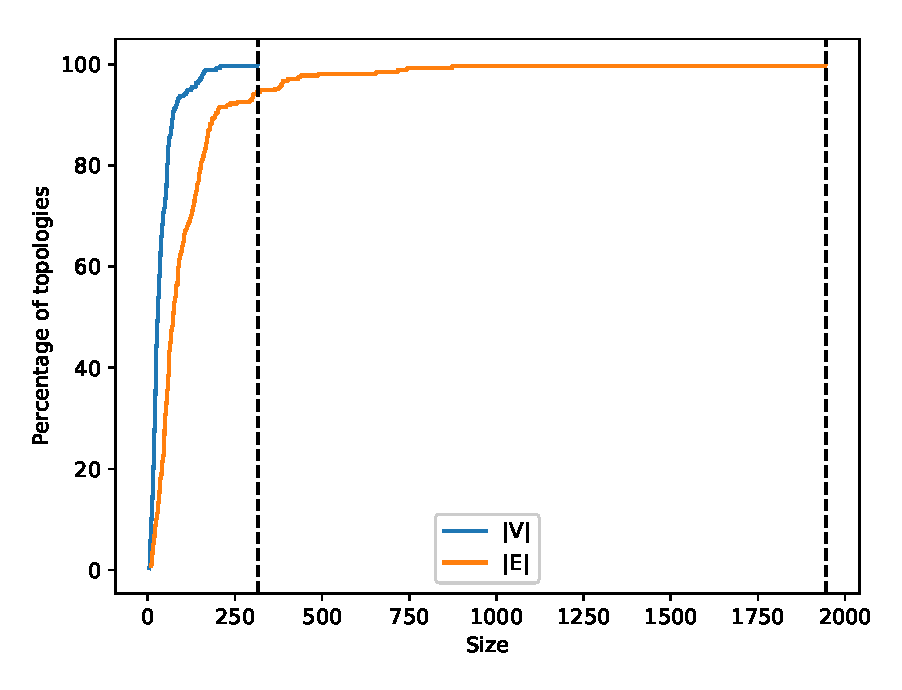
\includegraphics[width=.85\columnwidth]{./Network-lib/data/plot/topology_sizes.eps}
%\end{center}
%\caption{Distribution of the topology sizes.}
%\label{fig:sizes}
%\end{figure}

\begin{figure}
\begin{center}
\begin{tabular}{lrr}
\toprule
Topology name & $|V(G)|$ & $|E(G)|$\\
\midrule
AS 1221 & 104 & 302  \\
AS 1239 & 315 & 1944 \\
AS 1755 & 87 & 322   \\
AS 3257 & 161 & 656  \\
AS 3967 & 79 & 294   \\
AS 6461 & 138 & 744  \\
\bottomrule
\end{tabular}
\end{center}
\caption{Topology sizes in the \texttt{rf} group.}
\label{fig:rf_sizes}
\end{figure}

\begin{figure}
\begin{center}
\begin{tabular}{lrr}
\toprule
Topology name & $|V(G)|$ & $|E(G)|$\\
\midrule
ISP 1 & $\approx 150$ & $\approx 700$ \\
ISP 2 & $\approx 220$ & $\approx 800$ \\
ISP 3 & $\approx 170$ & $\approx 440$ \\
OVH   & 57 & 402 \\
\bottomrule
\end{tabular}
\end{center}
\caption{Topology sizes in the \texttt{real} group and \texttt{ovh}.}
\label{fig:real_sizes}
\end{figure}


\begin{figure}
\begin{center}
\begin{tabular}{lrr}
\toprule
Topology name & $|V(G)|$ & $|E(G)|$\\
\midrule
ITZ Cogentco  & 197 & 490 \\
ITZ Colt      & 153 & 382 \\
ITZ Deltacom  & 113 & 366 \\
ITZ Dia       & 138 & 302 \\
ITZ GtsCe     & 149 & 386 \\
ITZ Interoute & 110 & 312 \\
ITZ Ion       & 125 & 300 \\
ITZ Tata      & 145 & 388 \\
ITZ UsCarrier & 158 & 378 \\
\bottomrule
\end{tabular}
\end{center}
\caption{Largest topologies in the \texttt{zoo} group.}
\label{fig:zoo_sizes}
\end{figure}

\begin{figure}
\begin{center}
\begin{tabular}{cccc}
\toprule
Min $|V(G)|$ & Max $|V(G)|$ & Min $|E(G)|$ & Max $|E(G)|$ \\
\midrule
4 & 315 & 8 & 1955 \\
\bottomrule
\end{tabular}
\end{center}
\caption{Minimum and maximum topology sizes.}
\label{fig:sizes}
\end{figure}

\begin{figure}
\begin{center}
\begin{tabular}{cccc}
\toprule
Small & Medium & Large & Huge \\
$[0, 20]$ & $]20, 50]$ & $]50, 100]$ & $> 100$ \\
\midrule
30\% & 43\% & 21\% & 6\% \\
\bottomrule
\end{tabular}
\end{center}
\caption{Number of topologies by group size.}
\label{fig:group_sizes}
\end{figure}

\section{ECMP and non shortest path links}

We mentioned in the introduction that segment routing supports two kinds of segments: node segments 
and adjacency segments. We will see that adjacency segments are more costly and thus we would like to avoid using them whenever possible. However,
will see later that adjacency segments in segment routing can we necessary to implement paths that belong to ECMP components or that traverse
links that do not belong to any IGP shortest path. For that reason we analyzed the amount of ECMP component that exist in out dataset as well
as the amount of edges that do not belong to any shortest path. These values will give an estimation of how important supporting adjacency segments
is. Figure \ref{fig:ECMPcount} shows the percentage of links that do not belong to any shortest path as well as the percentage of pairs
of nodes with ECMP between them. We can see that, as expected, IGP weights are configured so that most links are used for shortest path routing, we
have only $1\%$ of the links falling outside of that.
We expect that mainly backup links will be configured so that they are not used unless a failure occurs. On the other hand, we see that
there is a relatively high percentage of pairs of nodes with ECMP. This indicates that adjacency segments will be useful whenever we want to
represent specific paths that traverse ECMP components. 

\begin{figure}
\begin{center}
\begin{tabular}{cccc}
\toprule
Links not in shortest paths & Pairs with ECMP \\
\midrule
$1\%$ & $26\%$  \\
\bottomrule
\end{tabular}
\end{center}
\caption{Percentage of links not in shortest paths and pairs with ECMP.}
\label{fig:ECMPcount}
\end{figure}

We also analyzed how many equal cost paths exist. Figure \ref{fig:ECMPcount} shows the CDF of the total number of shortest paths between each pair
of nodes over all topologies. This shows that some nodes are connected with a very high number of shortest paths but that most nodes have at most
$10$ shortest paths between them.

\begin{figure}
\begin{center}
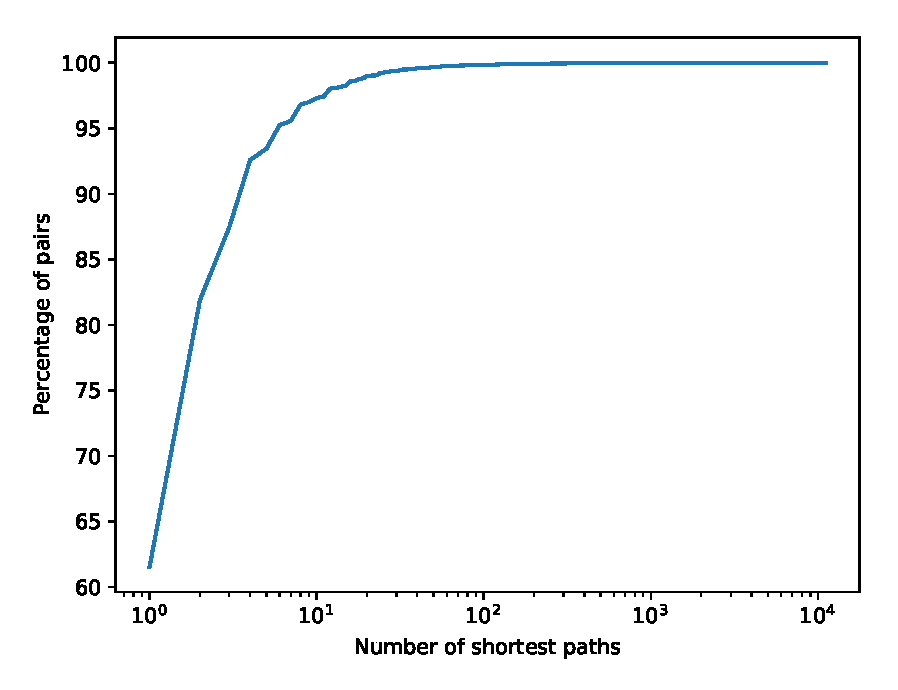
\includegraphics[width=.85\columnwidth]{./Network-lib/data/plot/spCount.eps}
\end{center}
\caption{CDF over all topologies and all pairs of nodes of the number of shortest paths between those nodes.}
\label{fig:maxEDP_boxplot}
\end{figure}

\section{Degrees and density}

We also analyzed the degrees of the nodes in the topologies in our dataset as well as the edge densities. The degree of a router represents the
number of routers to which it tis connected to. It represents an upper bound on the number of edge-disjoint paths that can be used to
connect a given router to other routers. Figure \ref{fig:deg_boxplot} shows a box plot of these. We can observe that some nodes have a very
high degree but that the tendency is that most nodes have a degree lower than $10$. Nodes of degree $1$ are problematic in a network
because it means that there is a single point of failure to reach them. We observe that the largest topologies are the ones that suffer the least
from this problem.

\begin{figure}
\begin{center}
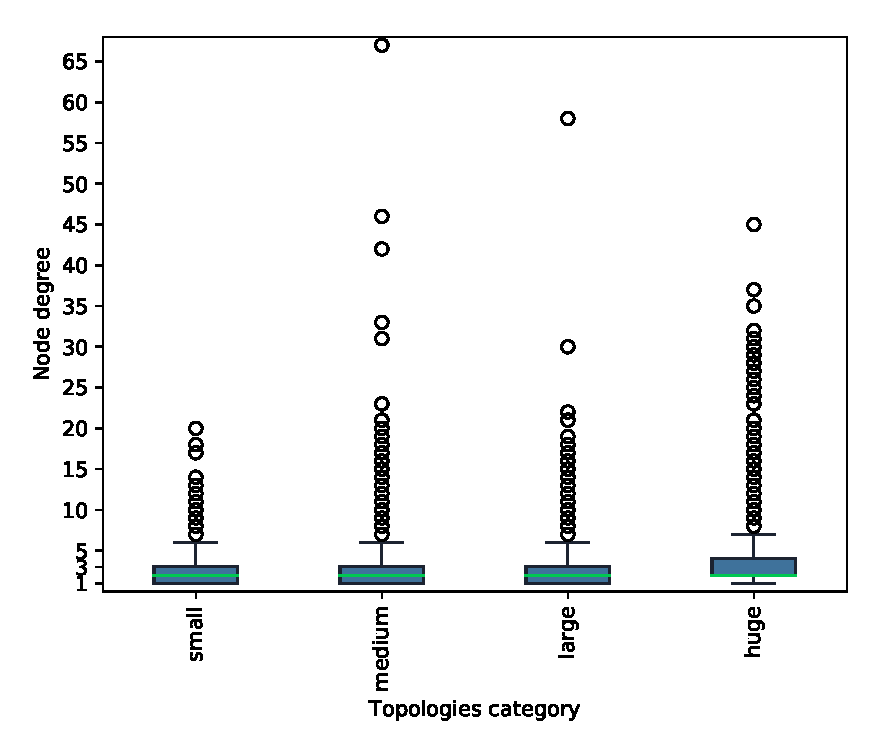
\includegraphics[width=.85\columnwidth]{./Network-lib/data/plot/deg_boxplot.eps}
\end{center}
\caption{Box plot of the degrees over the different size categories of our topologies.}
\label{fig:deg_boxplot}
\end{figure}

One degree nodes probably exist on these topologies due to the fact that most of them are were collected
using inexact methods thus leading to incomplete data. A computer network should at least be biconnected (have
at least two disjoint paths between every pair of nodes) to prevent a single link failure from partitioning
it.

The edge density of a network evaluates how close a network is from a complete graph. It is defined for graphs
with no parallel links as
$$
\frac{|E(G)|}{|V(G)| \cdot (|V(G)| - 1)}.
$$
A tree is the lowest density connected network that one can have. Any link failure in a tree will cause the network to become disconnected. High density network are costly but are more robust
to failures. They also provide a higher path diversity so optimal solution of network optimization problems tend to be
better on dense networks. Figure \ref{fig:density_cdf} shows a CDF of the densities over all topologies in
our dataset. We used the above formula even though some of our networks contain parallel links.
We can see that some network have a very low density. About $60\%$ percent of the network topologies
have an edge density of at least $10\%$ and $20\%$ of the networks have an edge density above $20\%$.

\begin{figure}
\begin{center}
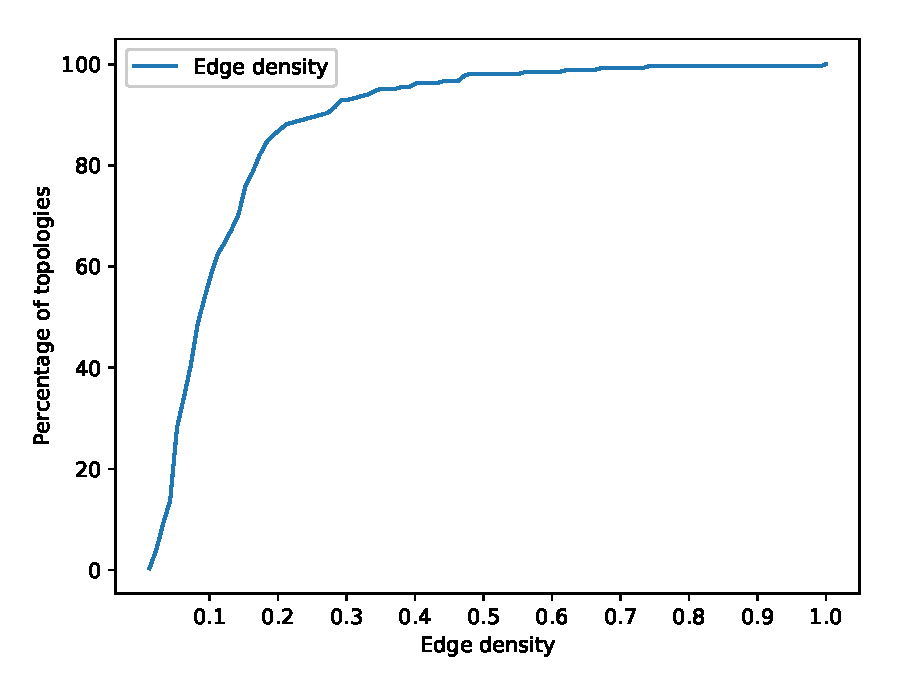
\includegraphics[width=.85\columnwidth]{./Network-lib/data/plot/edge_density.eps}
\end{center}
\caption{Box plot of the degrees over the different size categories of our topologies.}
\label{fig:density_cdf}
\end{figure}

\section{Connectivity}

We saw that some pairs of nodes have a lot of shortest paths between them. However these paths are of course not disjoint.
In this section we analyze how well the nodes are connected in the network. To measure this, we compute for each pair of nodes of each
topology the minimum number of links that need to be removed from the network in order to disconnect those nodes. This is known in graph
theory as the minimum cut between the nodes \cite{Ahuja}. Figure \ref{fig:mincut} shows a CDF of these minimum cuts. It is not hard to see
that the minimum cut between two nodes is the same as the maximum number of edge-disjoint paths between them \cite{Ahuja}.

\begin{figure}
\begin{center}
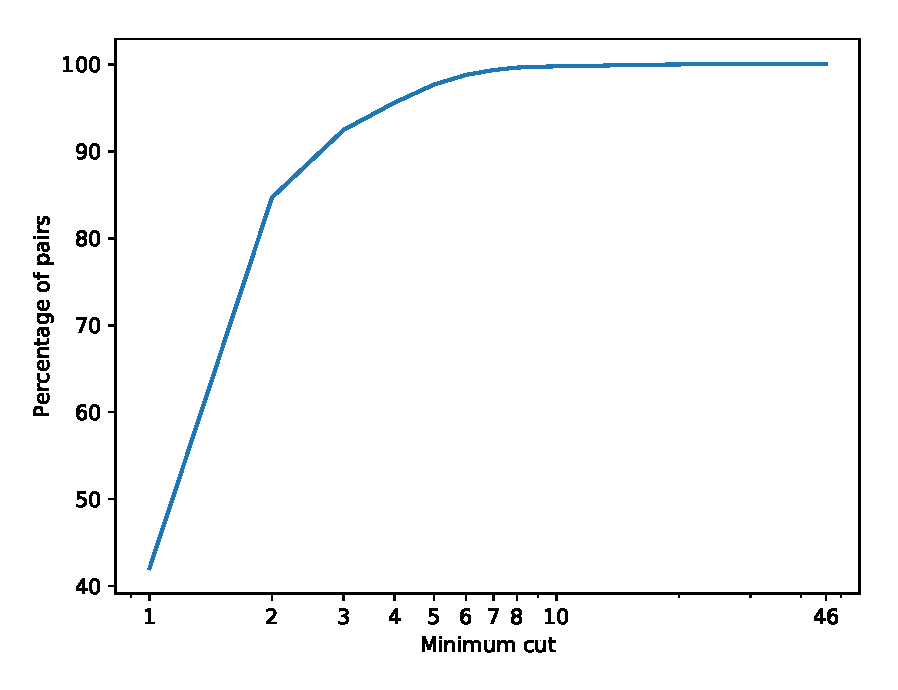
\includegraphics[width=.85\columnwidth]{./Network-lib/data/plot/minCuts.eps}
\end{center}
\caption{CDF over all topologies and all pairs of nodes of the number of shortest paths between those nodes.}
\label{fig:mincut}
\end{figure}

We can see that about $40\%$ of the pairs of nodes are connected by a single path as we had already observed above. This is quite low for a network as it does
not offer a lot of redundancy and link failures can easily disconnect the nodes. The remaining nodes require the removal of at least
$2$ links to disconnect them (in other words, they are in the same biconnected component \cite{Cormen:2009:IAT:1614191}). Also, nodes are very well connected having up to $46$ edge-disjoint paths connecting them.


\section*{Conclusion}

From this evaluation we observe that there is probably missing data on some of the topologies used in this
thesis as some of them are weakly connected. We have also seen that due to a high amout of ECMP ($26\%$) between pairs of nodes,
adjacency segments are likely to be necessary to implement paths in the graph topology with segment routing.

\chapter{Segment routing}
\label{chapter:sr}

\section*{Introduction}

As mentioned in the introduction, segment routing \cite{Filsfils_SR:2015} is a new forwarding architecture that is being developed within the Internet Engineering Task Force and network operators.
Segment Routing changes the way packets are forwarded
inside a network to enable network operators to have better
control on the path followed by the packets. Traffic can be forced to follow a series of detours
which can either correspond to passing by a specific router or network link.

This chapter is dedicated to formalizing segment routing. We provide, to the best of our knowledge, the first formalization that comprises
both node and adjacency segments. We define minimal segmentations and provide an efficient algorithm for computing 
them. We also provide reachability concepts which allow to analyze the capability of a given network topology
to support segment routing as well as giving lower bound on the minimum number of segments needed reach every single link
in the network. These concepts will be fundamental later on when we propose an algorithm for computing cycle covers 
of a network.

% Figure \ref{fig:srformal_sr1} illustrates an example of SR. In this example the ingress node is node 
% $\node{a}$ and there are two segments in the SR stack: an adjacent segment representing link $(\node{d}, \node{e})$
% and a node segment representing node $\node{i}$. We assume in the figure that all IGP weights are
% equal to $1$. The ingress node will look at the segment on the top of the stack and find link
% $(\node{d}, \node{e})$. It will then forward the packet to trough origin of the link, node $\node{d}$, through the shortest
% path $(\node{a}, \node{c}, \node{d})$. Then node $\node{d}$ will receive it an forward it to $\node{e}$ one the link $(\node{d}, \node{e})$.
% Node $\node{e}$ will then examine the segment stack see that the next segment is node $\node{i}$. It then
% forwards the packet to node $\node{i}$ via the shortest path $(\node{e}, \node{h}, \node{i})$.
% 
% \begin{figure}[H]
% \begin{center}
% \begin{tikzpicture}
% \def\x{0}
% \def\y{0}
% \node[scale=0.15] (a) at (0.5 + \x,  0.5 + \y) {\router{a}{green}};
% \node[scale=0.15] (b) at (0.5 + \x, -1.0 + \y) {\router{b}{lightgray}};
% \node[scale=0.15] (c) at (2.5 + \x,  0.0 + \y) {\router{c}{lightgray}};
% \node[scale=0.15] (d) at (4.5 + \x,  0.0 + \y) {\router{d}{green}};
% \node[scale=0.15] (e) at (4.0 + \x, -2.0 + \y) {\router{e}{green}};
% \node[scale=0.15] (g) at (6.0 + \x,  0.5 + \y) {\router{g}{lightgray}};
% \node[scale=0.15] (i) at (8.0 + \x,  0.0 + \y) {\router{i}{green}};
% \node[scale=0.15] (h) at (7.0 + \x, -1.5 + \y) {\router{h}{lightgray}};
% \node[scale=0.15] (f) at (4.0 + \x, -3.5 + \y) {\router{f}{lightgray}};
% \node[scale=0.15] (j) at (8.0 + \x, -2.5 + \y) {\router{j}{lightgray}};
% \draw[line width=2] (f) edge[above, sloped] node[black,font=\bfseries] {\tiny \texttt{}} (j);
% \draw[line width=2] (h) edge[above, sloped] node[black,font=\bfseries] {\tiny \texttt{}} (j);
% \draw[line width=2] (a) edge[above, sloped] node[black,font=\bfseries] {\tiny \texttt{}} (b);
% \draw[line width=2] (b) edge[above, sloped] node[black,font=\bfseries] {\tiny \texttt{}} (c);
% \draw[line width=2] (e) edge[above, sloped] node[black,font=\bfseries] {\tiny \texttt{}} (c);
% \draw[line width=2] (b) edge[above, sloped] node[black,font=\bfseries] {\tiny \texttt{}} (e);
% \draw[line width=2] (b) edge[above, sloped] node[black,font=\bfseries] {\tiny \texttt{}} (f);
% \draw[line width=2] (e) edge[above, sloped] node[black,font=\bfseries] {\tiny \texttt{}} (f);
% \draw[line width=2] (h) edge[above, sloped] node[black,font=\bfseries] {\tiny \texttt{}} (f);
% \draw[line width=2] (g) edge[above, sloped] node[black,font=\bfseries] {\tiny \texttt{}} (i);
% \draw[line width=2] (i) edge[above, sloped] node[black,font=\bfseries] {\tiny \texttt{}} (h);
% \draw[line width=2]  (d) edge[above, sloped] node[black,font=\bfseries] {\tiny \texttt{}} (g);
% \draw[line width=2]  (d) edge[above, sloped] node[black,font=\bfseries] {\tiny \texttt{}} (e);
% \draw[line width=2]  (e) edge[above, sloped] node[black,font=\bfseries] {\tiny \texttt{}} (h);
% \draw[line width=2]  (g) edge[above, sloped] node[black,font=\bfseries] {\tiny \texttt{}} (h);
% \draw[line width=2]  (c) edge[above, sloped] node[black,font=\bfseries] {\tiny \texttt{}} (d);
% \draw[line width=2]  (a) edge[above, sloped] node[black,font=\bfseries] {\tiny \texttt{}} (b);
% \draw[line width=2]  (a) edge[above, sloped] node[black,font=\bfseries] {\tiny \texttt{}} (c);
% 
% %%%%
% \draw (a) edge[line width=2, darkgreen, above, ->, bend right = 20] (c);
% \draw (c) edge[line width=2, darkgreen, above, ->, bend right = 20] (d);
% \draw (d) edge[line width=2, darkgreen, above, ->, dotted] (e);
% \draw (e) edge[line width=2, darkgreen, above, ->, bend left = 20] (h);
% \draw (h) edge[line width=2, darkgreen, above, ->, bend left = 20] (i);
% 
% 
% \def\x{-0.25}
% \def\y{1}
% \node at (\x + 2.2, \y + 0.25) {\footnotesize SR stack};
% \fill[lightgray] (\x, \y) rectangle (\x + 1.5, \y + 0.5);
% \fill[green] (\x, \y) rectangle (\x + 1, \y + 0.5);
% \draw[dotted, thick] (\x + 0.4, \y) -- (\x + 0.4, \y - 0.4);
% \draw[] (\x, \y) rectangle (\x + 1, \y + 0.5);
% \draw[] (\x, \y) rectangle (\x + 1.5, \y + 0.5);
% \draw (\x + 1, \y) -- (\x + 1, \y + 0.5);
% \node at (\x + 0.5, \y + 0.25) {\footnotesize $(d, e)$};
% \node at (\x + 1.25, \y + 0.28) {\footnotesize $i$};
% 
% \def\x{3.25}
% \def\y{-3}
% \fill[gray] (\x, \y) rectangle (\x + 1.5, \y + 0.5);
% \fill[green] (\x + 1, \y) rectangle (\x + 1.5, \y + 0.5);
% \draw[dotted, thick] (\x + 0.4, \y + 0.8) -- (\x + 0.4, \y + 0.5);
% \draw[] (\x, \y) rectangle (\x + 1, \y + 0.5);
% \draw[] (\x, \y) rectangle (\x + 1.5, \y + 0.5);
% \draw (\x + 1, \y) -- (\x + 1, \y + 0.5);
% \node at (\x + 0.5, \y + 0.25) {\footnotesize $(d, e)$};
% \node at (\x + 1.25, \y + 0.28) {\footnotesize $i$};
% 
% 
% \def\x{8 - 0.75}
% \def\y{0.5}
% \fill[gray] (\x, \y) rectangle (\x + 1.5, \y + 0.5);
% \draw[dotted, thick] (\x + 0.4, \y) -- (\x + 0.4, \y - 0.4);
% \draw[] (\x, \y) rectangle (\x + 1, \y + 0.5);
% \draw[] (\x, \y) rectangle (\x + 1.5, \y + 0.5);
% \draw (\x + 1, \y) -- (\x + 1, \y + 0.5);
% \node at (\x + 0.5, \y + 0.25) {\footnotesize $(d, e)$};
% \node at (\x + 1.25, \y + 0.28) {\footnotesize $i$};
% 
% 
% %%%%
% 
% %\def\x{-1}
% 
% %\draw[line width=2] (\x + 10, \y + -1 + 0.5) edge[] (\x + 10.5, \y + -1 + 0.5);
% %\node[anchor=west]  at (\x + 10.5, \y + -1 + 0.5) {\footnotesize network link};
% 
% %\draw[line width=2] (\x + 10, \y + -1) edge[dotted, darkgreen, ->] (\x + 10.5, \y + -1);
% %\node[anchor=west]  at (\x + 10.5, \y + -1) {\footnotesize adjacency segment};
% 
% %\draw[line width=2] (\x + 10, \y + -1 - 0.5) edge[] (\x + 10.5, \y + -1 - 0.5);
% %\node[anchor=west]  at (\x + 10.5, \y + -1 - 0.5) {\footnotesize s link};
% 
% 
% \end{tikzpicture}
% \end{center}
% \caption{Illustration of SR with segments $(d, e)$ and $i$ and ingress node $a$. Dashed arrows represent adjacency segments
% and the others represent the shortest path edges between consecutive segments.}
% \label{fig:srformal_sr1}
% \end{figure}
% 
% This chapter is organized as follows. We start in Section \ref{section:sr-formal} by providing a formalization
% of segment routing. To the best of our knowledge, this is the first work that studies segment routing in
% 
% \todo{finish chapter organization}
% 
% \todo{we need to explain that when the graph is undirected we don't draw both arrows}


\section{Segment routing formalization}

\label{section:sr-formal}

The starting point of our segment routing formalization is the concept of segment routing path, or sr-path for short.

\begin{definition}
Let $G$ be a network. A \emph{sr-path} $\sr{p}$ on $G$ is a sequence $\langle x_1, \ldots, x_l \rangle$ such that each $x_i \in V(G) \cup E(G)$.
%We use the notation $\sr{p}_i = x_i$ to represent the $i$-th element in the sequence.
\end{definition}

We represent sr-paths with the vector notation to be able to more easily distinguish between a path $p$ and a 
sr-path $\sr{p}$ in the network $G$. In practice, the elements of $\sr{p}$ that are nodes model node segments and
the elements of $\sr{p}$ that are edges model adjacency segments. It is important to understand that, because of ECMP, a sr-path
actually can correspond to a set of paths in the original network. 

Consider the sr-path $\sr{p} = \langle \node{a}, \node{c}, \node{e}, (\node{f}, \node{j}), \node{i} \rangle$ shown in
Figure \ref{fig:sr-path}. The solid green edges show the set of edges that belong to shortest paths between consecutive segments
and the dashed green edge represents the adjacency segment $(\node{f}, \node{j})$. The square boxes represent segments. The box is represented next to
a node for node segments and on top of the link of an adjacency segment. So, in this case, $x_1 = \node{a}, x_2 = \node{c}, x_3 = \node{e}, x_4 = \edge{f}{j}$
and $x_5 = \node{i}$.

In this example, between nodes \node{c} and \node{e} there are two shortest paths, namely
$((\node{c}, \node{d}), (\node{d}, \node{e}))$ and $((\node{c}, \node{b}), (\node{b}, \node{e}))$. In the same way,
two shortest paths exist between nodes \node{e} and \node{f} because we have two parallel links with the same IGP weight
between them. In each case, any of those two paths could be used to forward packets over this
sr-path. Thus, we see that the sr-path $\sr{p}$ can correspond to four paths over the original network, namely,

\begin{align*}
((\node{a}, \node{c}), (\node{c}, \node{d}), (\node{d}, \node{e}), (\node{e}, \node{f}, i_1), (\node{f}, \node{j}), (\node{j}, \node{h}), (\node{h}, \node{i})), \\
((\node{a}, \node{c}), (\node{c}, \node{d}), (\node{d}, \node{e}), (\node{e}, \node{f}, i_2), (\node{f}, \node{j}), (\node{j}, \node{h}), (\node{h}, \node{i})), \\
((\node{a}, \node{c}), (\node{c}, \node{b}), (\node{b}, \node{e}), (\node{e}, \node{f}, i_1), (\node{f}, \node{j}), (\node{j}, \node{h}), (\node{h}, \node{i})), \\
((\node{a}, \node{c}), (\node{c}, \node{b}), (\node{b}, \node{e}), (\node{e}, \node{f}, i_2), (\node{f}, \node{j}), (\node{j}, \node{h}), (\node{h}, \node{i})) \\
\end{align*}

where $(\node{e}, \node{f}, i_1)$ and $(\node{e}, \node{f}, i_2)$ represent the two links between $\node{e}$ and $\node{f}$.

\begin{figure}
\begin{center}
\begin{tikzpicture}
\def\x{0}
\def\y{0}
\node[scale=0.15] (a) at (0.5 + \x,  0.5 + \y) {\router{a}{marked}};
\node[scale=0.15] (b) at (0.5 + \x, -1.0 + \y) {\router{b}{router}};
\node[scale=0.15] (c) at (2.5 + \x,  0.0 + \y) {\router{c}{marked}};
\node[scale=0.15] (d) at (4.5 + \x,  0.0 + \y) {\router{d}{router}};
\node[scale=0.15] (e) at (4.0 + \x, -2.0 + \y) {\router{e}{marked}};
\node[scale=0.15] (g) at (6.0 + \x,  0.5 + \y) {\router{g}{router}};
\node[scale=0.15] (i) at (8.0 + \x,  0.0 + \y) {\router{i}{marked}};
\node[scale=0.15] (h) at (7.0 + \x, -1.5 + \y) {\router{h}{router}};
\node[scale=0.15] (f) at (4.0 + \x, -3.5 + \y) {\router{f}{router}};
\node[scale=0.15] (j) at (8.0 + \x, -2.5 + \y) {\router{j}{router}};
\draw[line width=2] (f) edge[above, sloped] node[black,font=\bfseries] {\tiny \texttt{}} (j);
\draw[line width=2] (h) edge[above, sloped] node[black,font=\bfseries] {\tiny \texttt{}} (j);
\draw[line width=2] (a) edge[above, sloped] node[black,font=\bfseries] {\tiny \texttt{}} (b);
\draw[line width=2] (b) edge[above, sloped] node[black,font=\bfseries] {\tiny \texttt{}} (c);
\draw[line width=2] (b) edge[above, sloped] node[black,font=\bfseries] {\tiny \texttt{}} (e);
\draw[line width=2] (b) edge[above, sloped] node[black,font=\bfseries] {\tiny \texttt{}} (f);
\draw[line width=2] (e) edge[above, sloped, bend left=10] node[black,font=\bfseries] {\tiny \texttt{}} (f);
\draw[line width=2] (e) edge[above, sloped, bend right=10] node[black,font=\bfseries] {\tiny \texttt{}} (f);
\draw[line width=2] (h) edge[above, sloped] node[black,font=\bfseries] {\tiny \texttt{}} (f);
\draw[line width=2] (g) edge[above, sloped] node[black,font=\bfseries] {\tiny \texttt{}} (i);
\draw[line width=2] (i) edge[above, sloped] node[black,font=\bfseries] {\tiny \texttt{}} (h);
\draw[line width=2]  (d) edge[above, sloped] node[black,font=\bfseries] {\tiny \texttt{}} (g);
\draw[line width=2]  (d) edge[above, sloped] node[black,font=\bfseries] {\tiny \texttt{}} (e);
\draw[line width=2]  (e) edge[above, sloped] node[black,font=\bfseries] {\tiny \texttt{}} (h);
\draw[line width=2]  (g) edge[above, sloped] node[black,font=\bfseries] {\tiny \texttt{}} (h);
\draw[line width=2]  (c) edge[above, sloped] node[black,font=\bfseries] {\tiny \texttt{}} (d);
\draw[line width=2]  (a) edge[above, sloped] node[black,font=\bfseries] {\tiny \texttt{}} (b);
\draw[line width=2]  (a) edge[above, sloped] node[black,font=\bfseries] {\tiny \texttt{}} (c);

%%%%
\draw (a) edge[line width=3, darkgreen, above, ->, bend left = 20] (c);
\draw (c) edge[line width=3, darkgreen, above, ->, bend right = 20] (d);
\draw (c) edge[line width=3, darkgreen, above, ->, bend right = 20] (b);
\draw (b) edge[line width=3, darkgreen, above, ->, bend left = 20] (e);
\draw (d) edge[line width=3, darkgreen, above, ->, bend right = 20] (e);

\draw (j) edge[line width=3, darkgreen, above, ->, bend left = 20] (h);
\draw (f) edge[line width=4, darkgreen, ->, dotted] node[line width = 1, draw, solid, black, fill=green] {\footnotesize $x_4$} (j);

\draw (h) edge[line width=3, darkgreen, above, ->, bend left = 20] (i);
\draw (e) edge[line width=3, darkgreen, above, ->, bend right = 30] (f);
\draw (e) edge[line width=3, darkgreen, above, ->, bend left = 30] (f);

\node[left = 0.1cm of a, draw, fill=green] {\footnotesize $x_1$};
\node[above = 0.1cm of c, draw, fill=green] {\footnotesize $x_2$};
\node[above right = 0.1cm of e, draw, fill=green] {\footnotesize $x_3$};
\node[right = 0.1cm of i, draw, fill=green] {\footnotesize $x_4$};

\end{tikzpicture}
\end{center}
\caption{Illustration of sr-path $\sr{p} = \langle \node{a}, \node{c}, \node{e}, (\node{f}, \node{j}), \node{i} \rangle$.}
\label{fig:sr-path}
\end{figure}


In general, when we use a sr-path $\sr{p} = \langle x_1, \ldots, x_l \rangle$ to forward traffic, between segments $x_i$ and $x_{i + 1}$ the set of paths
over which this traffic might be sent corresponds to the set of all shortest paths between those segments. In this thesis we consider two models for
forwarding traffic over ECMP:

\begin{enumerate}
 \item \emph{Hash model}: Whenever several next-hops exists with respect to the IGP shortest paths, a hash function is used to select which of them is used.
 This hash function is unknown and depends on the traffic that is sent. From a practical point of view this, more or less, corresponds to assuming that one of the
 multiple shortest paths is selected at random.
 
 \item \emph{Split model}: The traffic is split evenly between all shortest paths. This means that if, for instance, a router contains two next-hops, it will forward
 $50\%$ of the traffic towards one of them and the other $50\%$ towards the other.
\end{enumerate}


But these segments, $x_i$ and $x_{i + 1}$ might not both correspond to nodes in which case we need to give a precise definition of what the set of shortest paths between two segments means. 
In general, we have four cases which are summarized
in Figure \ref{fig:4case-sr}. If we have two node segments $x_i = v, x_{i + 1} = u$ then it is the subgraph between $v$ and $u$, $\sp(v, u)$. 
If $x_i = v$ and $x_{i + 1} = (u_1, u_2)$ then it the subgraph between $v$ and $u_1$, $\sp(v, u_1)$. If $x_i = (v_1, v_2)$ and $x_{i + 1} = u$ then it is
the shortest path subgraph between $v_2$ and $u$. Finally, if both are adjacency segments with $x_i = (v_1, v_2)$ and $x_{i + 1} = (u_1, u_2)$ then it is
$\sp(v_2, u_1)$.

\begin{figure}[H]
\begin{center}
\begin{tabular}{c}
\begin{tikzpicture}
\node[scale=0.15] (v) at (0, 0) {\router{$v$}{marked}};
\node[scale=0.15] (u) at (3, 0) {\router{$u$}{marked}};
\path (v) edge[line width=2, darkgreen, out=-30, in=240, wavy, ->] (u);
\path (v) edge[line width=2, darkgreen, out=30, in=150, wavy, ->] (u);
\node at (0, 1) {$x_i = v$};
\node at (3, 1) {$x_{i+1} = u$};
\node[darkgreen,font=\bfseries] at (1.5, 0) {$\sp(v, u)$};
\end{tikzpicture}
\\
\emph{Case 1:} $x_i$ and $x_{i + 1}$ are both node segments
\\[0.5cm]
\begin{tikzpicture}
\node[scale=0.15] (v) at (0, 0) {\router{$v$}{marked}};
\node[scale=0.15] (u1) at (3, 0) {\router{$u_1$}{router}};
\node[scale=0.15] (u2) at (5, 0) {\router{$u_2$}{router}};
\path (v) edge[line width=2, darkgreen, out=-30, in=240, wavy, ->] (u1);
\path (v) edge[line width=2, darkgreen, out=30, in=150, wavy, ->] (u1);
\draw[line width=2]  (u1) edge[above, sloped] node[black,font=\bfseries] (l) {} (u2);
\draw (u1) edge[line width=4, darkgreen, above, ->, dotted] (u2);
\node at (0, 1) {$x_i = v$};
\node at (4, 1) {$x_{i+1} = (u_1, u_2)$};
\node[darkgreen,font=\bfseries] at (1.5, 0) {$\sp(v, u_1)$};
\end{tikzpicture}
\\
\emph{Case 2:} $x_i$ is a node segment and $x_{i + 1}$ is an adjacency segment
\\[0.5cm]
\begin{tikzpicture}
\node[scale=0.15] (v1) at (0, 0) {\router{$v_1$}{router}};
\node[scale=0.15] (v2) at (2, 0) {\router{$v_2$}{router}};
\node[scale=0.15] (u) at (5, 0) {\router{$u$}{marked}};
\path (v2) edge[line width=2, darkgreen, out=-30, in=240, wavy, ->] (u);
\path (v2) edge[line width=2, darkgreen, out=30, in=150, wavy, ->] (u);
\draw[line width=2]  (v1) edge[above, sloped] node[black,font=\bfseries] (l) {} (v2);
\draw (v1) edge[line width=4, darkgreen, above, ->, dotted] (v2);
\node at (1, 1) {$x_i = (v_1, v_2)$};
\node at (5, 1) {$x_{i+1} = u$};
\node[darkgreen,font=\bfseries] at (3.5, 0) {$\sp(v_2, u)$};
\end{tikzpicture}
\\
\emph{Case 3:} $x_i$ is an adjacency segment and $x_{i + 1}$ is a node segment
\\[0.5cm]
\begin{tikzpicture}
\node[scale=0.15] (v1) at (0, 0) {\router{$v_1$}{router}};
\node[scale=0.15] (v2) at (2, 0) {\router{$v_2$}{router}};
\node[scale=0.15] (u1) at (5, 0) {\router{$u_1$}{router}};
\node[scale=0.15] (u2) at (7, 0) {\router{$u_2$}{router}};
\path (v2) edge[line width=2, darkgreen, out=-30, in=240, wavy, ->] (u1);
\path (v2) edge[line width=2, darkgreen, out=30, in=150, wavy, ->] (u1);
\draw[line width=2]  (v1) edge[above, sloped] node[black,font=\bfseries] (l) {} (v2);
\draw (v1) edge[line width=4, darkgreen, above, ->, dotted] (v2);
\draw[line width=2]  (u1) edge[above, sloped] node[black,font=\bfseries] (l) {} (u2);
\draw (u1) edge[line width=4, darkgreen, above, ->, dotted] (u2);
\node at (1, 1) {$x_i = (v_1, v_2)$};
\node at (6, 1) {$x_{i+1} = (u_1, u_2)$};
\node[darkgreen,font=\bfseries] at (3.5, 0) {$\sp(v_2, u_1)$};
\end{tikzpicture}
\\
\emph{Case 4:} $x_i$ and $x_{i + 1}$ are both adjacency segments
\end{tabular}
\end{center}
\caption{Shortest paths between consecutive segments.}
\label{fig:4case-sr}
\end{figure}

Having to deal with these four cases would be very cumbersome. When considering a sr-path $\sr{p}$ we want to have a way to
ignore as much as possible the nature of each of the segments. This will make proving results involving sr-paths easier and also
will ease the readability of proofs. This lead us to define the following notation so that we can
very simply capture all four cases.

\begin{definition}
Let $G$ be a network and $\sr{p} = \langle x_1, \ldots, x_l \rangle$. If $x_i \in V(G)$ we define $x^1_i = x^2_i = x_i$ and
if $x_i = (u_1, u_2) \in E(G)$ we define $x^1_i = u_1$ and $x^2_i = u_2$. 
\end{definition}

With this notation, we can now simply say that the set of shortest paths between two consecutive segments $x_i$ and $x_{i + 1}$
of a sr-path $\sr{p}$ is the subgraph $\sp(x^2_i, x^1_{i + 1})$. This works regardless of what the type of segments $x_i$ and $x_{i + 1}$
are. This notation also makes it easy to refer to the starting and ending routers of a sr-path.

\begin{definition}
Let $G$ be a network and $\sr{p} = \langle x_1, \ldots, x_l \rangle$. We say that $\sr{p}$ is a sr-path from node $x^1_1$ to
$x^2_l$. We say that $x^1_1$ is the first node of $\sr{p}$ and $x^2_l$ is the last node of $\sr{p}$. A sr-path that
starts and ends at the same node is called a sr-cycle.
\end{definition}

As we mentioned in the introduction of this chapter, when we use segment routing as a forwarding mechanism, we need to append to the packet 
header the segments that are to be used. Commercial routers have strong limitations regarding the size of this header. Some routers can
support sr-paths with up to $10$ segments but on average this number is closer to $5$ \cite{Tantsura_SID:2017}.
This means that it is important to be able to capture the cost, in terms of segments, of a sr-path. A node segment needs to contain
the IP address of the corresponding router whereas an adjacency segment needs the IP address of the source node of the corresponding link
as well as the interface identifier of that link. For this reason, we model the cost of individual segments and sr-paths as follows.

\begin{definition}
Let $G$ be a network and $\sr{p} = \langle x_1, \ldots x_l \rangle$ a sr-path on $G$. We define the cost of $x_i$ as
\[ \cost(x_i) =
  \begin{cases}
    1 & \quad \text{if } x_{i} \in V(G) \\
    2 & \quad \text{otherwise}
  \end{cases}
\]
We define the \emph{segment cost} of $\sr{p}$ as
$$
\cost(\sr{p}) = \sum_{i = 1}^l \cost(x_i)
$$
\end{definition}

Note that this model does not exactly match the reality. In practice, if the first segment is a node segment, its IP address will never be put into the
segment stack. Also, if the first segment is an adjacency segment only the link interface would be necessary
for the same reason. We chose to ignore this and count each segment equally because it greatly simplifies the mathematical developments. Furthermore, we
believe that the model is close enough that this will have a minor impact in practice. In the worst case, we overestimate the real segment cost
of a sr-path by $1$.

\begin{definition}
Let $G$ be a network. We denote the set of all sr-paths on $G$ by $\sr{\mathcal{P}}$. Given $k \in \mathbb{N}$ we define
$$
\mathcal{\sr{P}}_k(G) = \left\{ \sr{p} \mid \text{$\sr{p}$ is a sr-path on $G$ and $\cost(\sr{p}) \leq k$} \right\}.
$$
Finally, given $s, t \in V(G)$ we denote the set of all sr-paths from $s$ to $t$ of segment cost at most $k$
by $\Pk(s, t)$.

\end{definition}

We now define some operations on sr-paths and prove some of theirs properties.
 
\begin{definition}
Let $G$ be a network and $\sr{p} = \langle x_1, \ldots, x_l \rangle, \sr{q} = \langle y_1, \ldots, y_r \rangle$ be two sr-paths on $G$. We 
define the sum of $\sr{p}$ and $\sr{q}$ as
$$
\sr{p} + \sr{q} = \langle x_1, \ldots, x_l, y_1, \ldots, y_r \rangle
$$
\end{definition}

\begin{lemma}
\label{lemma:srsumcost}
Let $G$ be a network and $\sr{p} = \langle x_1, \ldots, x_l \rangle, \sr{q} = \langle y_1, \ldots, y_r \rangle$ be two sr-paths on $G$. Then
$$
\cost(\sr{p} + \sr{q}) = \cost(\sr{p}) + \cost(\sr{q}) 
$$
\end{lemma}

\begin{proof}
\begin{align*}
\cost(\sr{p} + \sr{q}) & = \cost(\langle x_1, \ldots, x_l, y_1, \ldots, y_r) \\
& = \sum_{i = 1}^l \cost(x_i) + \sum_{i = 1}^r \cost(y_i) \\
& = \cost(\sr{p}) + \cost(\sr{q})
\end{align*}
\end{proof}

Addition of sr-paths will turn out to be useful to prove
bounds on the segment cost of sr-paths produced by some of our algorithms. However, 
addition of sr-paths does not care about the segments contained in each path. It simply takes all segments
from both paths and put them in order into a single sr-path. For example, it could be the case that $x_l = y_1$
so the resulting sr-path would have a segment repeated twice next to each other. This does not 
cause any practical problem but in terms of routing it is redundant. Moreover, it wastes space in the segment stack. This can be the case even if $x_l \neq y_1$ but the last node of $x_l$ and the first node of $y_1$ 
are the same, that is, if $x^2_l = y^1_1$. For instance let $\sr{p} = \langle \node{a}, \node{f} \rangle$ and
$\sr{q} = \langle (\node{f}, \node{j}), \node{i} \rangle$. Then 
$\sr{p} + \sr{q} = \langle \node{a}, \node{f}, (\node{f}, \node{j}), \node{i} \rangle$. 
In terms of routing, this sr-path traverses the same links as the sr-path $\langle \node{a}, (\node{f}, \node{j}), \node{i} \rangle$
but it costs one more because it has a useless node segment on $\node{f}$.
With this in mind, we define a concatenation operation $\oplus$ on sr-paths which takes this into account and discards useless segments at the concatenation
point in the resulting sr-path.

% \begin{figure}[H]
% \begin{center}
% \begin{tikzpicture}
% \def\x{0}
% \def\y{0}
% \node[scale=0.15] (a) at (0.5 + \x,  0.5 + \y) {\router{a}{green}};
% \node[scale=0.15] (b) at (0.5 + \x, -1.0 + \y) {\router{b}{router}};
% \node[scale=0.15] (c) at (2.5 + \x,  0.0 + \y) {\router{c}{router}};
% \node[scale=0.15] (d) at (4.5 + \x,  0.0 + \y) {\router{d}{router}};
% \node[scale=0.15] (e) at (4.0 + \x, -2.0 + \y) {\router{e}{router}};
% \node[scale=0.15] (g) at (6.0 + \x,  0.5 + \y) {\router{g}{router}};
% \node[scale=0.15] (i) at (8.0 + \x,  0.0 + \y) {\router{i}{green}};
% \node[scale=0.15] (h) at (7.0 + \x, -1.5 + \y) {\router{h}{router}};
% \node[scale=0.15] (f) at (4.0 + \x, -3.5 + \y) {\router{f}{green}};
% \node[scale=0.15] (j) at (8.0 + \x, -2.5 + \y) {\router{j}{green}};
% \draw[line width=2] (f) edge[above, sloped] node[black,font=\bfseries] {\tiny \texttt{}} (j);
% \draw[line width=2] (h) edge[above, sloped] node[black,font=\bfseries] {\tiny \texttt{}} (j);
% \draw[line width=2] (a) edge[above, sloped] node[black,font=\bfseries] {\tiny \texttt{}} (b);
% \draw[line width=2] (b) edge[above, sloped] node[black,font=\bfseries] {\tiny \texttt{}} (c);
% \draw[line width=2] (b) edge[above, sloped] node[black,font=\bfseries] {\tiny \texttt{}} (e);
% \draw[line width=2] (b) edge[above, sloped] node[black,font=\bfseries] {\tiny \texttt{}} (f);
% \draw[line width=2] (e) edge[above, sloped, bend left=10] node[black,font=\bfseries] {\tiny \texttt{}} (f);
% \draw[line width=2] (e) edge[above, sloped, bend right=10] node[black,font=\bfseries] {\tiny \texttt{}} (f);
% \draw[line width=2] (h) edge[above, sloped] node[black,font=\bfseries] {\tiny \texttt{}} (f);
% \draw[line width=2] (g) edge[above, sloped] node[black,font=\bfseries] {\tiny \texttt{}} (i);
% \draw[line width=2] (i) edge[above, sloped] node[black,font=\bfseries] {\tiny \texttt{}} (h);
% \draw[line width=2]  (d) edge[above, sloped] node[black,font=\bfseries] {\tiny \texttt{}} (g);
% \draw[line width=2]  (d) edge[above, sloped] node[black,font=\bfseries] {\tiny \texttt{}} (e);
% \draw[line width=2]  (e) edge[above, sloped] node[black,font=\bfseries] {\tiny \texttt{}} (h);
% \draw[line width=2]  (g) edge[above, sloped] node[black,font=\bfseries] {\tiny \texttt{}} (h);
% \draw[line width=2]  (c) edge[above, sloped] node[black,font=\bfseries] {\tiny \texttt{}} (d);
% \draw[line width=2]  (a) edge[above, sloped] node[black,font=\bfseries] {\tiny \texttt{}} (b);
% \draw[line width=2]  (a) edge[above, sloped] node[black,font=\bfseries] {\tiny \texttt{}} (c);
% 
% %%%%
% \draw (a) edge[line width=3, darkgreen, above, ->, bend right = 20] (b);
% \draw (b) edge[line width=3, darkgreen, above, ->, bend right = 20] (f);
% 
% \draw (j) edge[line width=3, darkgreen, above, ->, bend left = 20] (h);
% \draw (f) edge[line width=4, darkgreen, above, ->, dotted] (j);
% 
% \draw (h) edge[line width=3, darkgreen, above, ->, bend left = 20] (i);
% 
% \end{tikzpicture}
% \end{center}
% \label{fig:sr-add}
% \caption{Illustration of sr-path $\sr{p} + \sr{q} = \langle \node{a}, \node{f} \rangle + \langle (\node{f}, \node{j}), \node{i} \rangle = \langle \node{a}, \node{f}, (\node{f}, \node{j}), \node{i} \rangle$.}
% \end{figure}

\begin{definition}
\label{def:sr-concat}
Let $G$ be a network and $\sr{p} = \langle x_1, \ldots, x_l \rangle$ be a sr-path from
$a$ to $b$ and $\sr{q} = \langle y_1, \ldots, y_r \rangle$ be a sr-path from $b$ to $c$, where $a, b, c \in V(G)$.
We  define the concatenation of $\sr{p}$ and $\sr{q}$ as
\[ \sr{p} \oplus \sr{q} =
  \begin{cases}
    \langle x_1, \ldots, x_l, y_2, \ldots, y_r \rangle & \quad \text{if } x_l = y_1 = b \in V(G) \\
    \langle x_1, \ldots, x_l, y_2, \ldots, y_r \rangle & \quad \text{if } x_l \in E(G) \text{ and } y_1 \in V(G) \\
    \langle x_1, \ldots, x_{l - 1}, y_1, \ldots, y_r \rangle & \quad \text{if } x_l \in V(G) \text{ and } y_1 \in E(G) \\
    \langle x_1, \ldots, x_l, y_1, \ldots, y_r \rangle & \quad \text{if } x_l \in E(G) \text{ and } y_1 \in E(G) \\
  \end{cases}
\]
\end{definition}

With sr-path concatenation we avoid consecutive redundant segments by removing them if necessary beforehand.
For the above example with $\sr{p} = \langle \node{a}, \node{f} \rangle$ and
$\sr{q} = \langle (\node{f}, \node{j}), \node{i} \rangle$ we have 
$\sr{p} \oplus \sr{q} = \langle \node{a}, (\node{f}, \node{j}), \node{i} \rangle$. Figure \ref{fig:sr-concat}
illustrates the four cases of sr-path concatenation from Definition \ref{def:sr-concat}.

\begin{figure}[H]
\begin{center}
\begin{tabular}{c}
\begin{tikzpicture}
\draw[cyan, ultra thick] (-3.5, -0.5) rectangle (0.6, 0.5);
\draw[orange, ultra thick] (1.4, -0.5) rectangle (5.5, 0.5);

\node[scale=0.15] (v) at (0, 0) {\router{$b$}{router}};
\node[scale=0.15] (u) at (2, 0) {\router{$b$}{router}};
\node at (0, 1) {$x_l = b$};
\node at (2, 1) {$y_{1} = b$};
\node[left of=v] {\large $\ldots$};
\node[right of=u] {\large $\ldots$};

\node at (1, 0) {\large $\oplus$};
\node[rotate=-90] at (1, -0.75) {\large $\rightarrowtail$};

\node[scale=0.15] (b) at (1, -1.5) {\router{$b$}{router}};
\node[left of=b] {\large $\ldots$};
\node[right of=b] {\large $\ldots$};

\draw[cyan, ultra thick] (-2.7, -2) rectangle (1.7, -1);
\draw[orange, ultra thick] (0.3, -2) rectangle (4.7, -1);

\end{tikzpicture}
\\[0.25cm]
\emph{Case 1:} $x_l = y_1 = b \in V$
\\[1cm]
\begin{tikzpicture}
\draw[cyan, ultra thick] (-3.5, -0.5) rectangle (0.6, 0.5);
\draw[orange, ultra thick] (1.4, -0.5) rectangle (5.5, 0.5);

\node[scale=0.15] (v) at (0, 0) {\router{$b$}{router}};
\node[scale=0.15] (u1) at (2, 0) {\router{$b$}{router}};
\node[scale=0.15] (u2) at (4, 0) {\router{$*$}{router}};
\draw[line width=2]  (u1) edge[above, sloped] node[black,font=\bfseries] (l) {} (u2);
\draw (u1) edge[line width=4, darkgreen, above, ->, dotted] (u2);
\node at (0, 1) {$x_l = b$};
\node at (3, 1) {$y_1 = (b, *)$};
\node at (1, 0) {\large $\oplus$};

\node[left of=v] {\large $\ldots$};
\node[right of=u2] {\large $\ldots$};
\node[rotate=-90] at (3, -0.75) {\large $\rightarrowtail$};

\node[scale=0.15] (x) at (3, -1.5) {\router{$*$}{router}};
\node[scale=0.15] (b) at (1, -1.5) {\router{$b$}{router}};
\node[left of=b] {\large $\ldots$};
\node[right of=x] {\large $\ldots$};
\draw[line width=2] (b) edge[above, sloped] (x);
\draw (b) edge[line width=4, darkgreen, above, ->, dotted] (x);

\draw[cyan, ultra thick] (-2.7, -2) rectangle (1.7, -1);
\draw[orange, ultra thick] (0.3, -2) rectangle (4.7, -1);

\end{tikzpicture}
\\[0.25cm]
\emph{Case 2:} $x_l \in E(G)$, $y_{1} \in V(G)$ and $x^2_l =  y_1 = b$
\\[1cm]
\begin{tikzpicture}
\draw[cyan, ultra thick] (-1.5, -0.5) rectangle (2.6, 0.5);
\draw[orange, ultra thick] (3.4, -0.5) rectangle (7.5, 0.5);

\node[scale=0.15] (v1) at (0, 0) {\router{$x$}{router}};
\node[scale=0.15] (v2) at (2, 0) {\router{$b$}{router}};
\node[scale=0.15] (u) at (4, 0) {\router{$b$}{router}};
\draw[line width=2]  (v1) edge[above, sloped] node[black,font=\bfseries] (l) {} (v2);
\draw (v1) edge[line width=4, darkgreen, above, ->, dotted] (v2);
\node at (1, 1) {$x_l = (*, b)$};
\node at (4, 1) {$y_1 = b$};
\node at (3, 0) {\large $\oplus$};

\node[left of=v1] {\large $\ldots$};
\node[right of=u] {\large $\ldots$};
\node[rotate=-90] at (3, -0.75) {\large $\rightarrowtail$};

\node[scale=0.15] (x) at (1, -1.5) {\router{$x$}{router}};
\node[scale=0.15] (b) at (3, -1.5) {\router{$b$}{router}};
\node[left of=x] {\large $\ldots$};
\node[right of=b] {\large $\ldots$};
\draw[line width=2] (x) edge[above, sloped] (b);
\draw (x) edge[line width=4, darkgreen, above, ->, dotted] (b);
\draw[cyan, ultra thick] (-0.5, -2) rectangle (3.7, -1);
\draw[orange, ultra thick] (2.3, -2) rectangle (6.5, -1);

\end{tikzpicture}
\\[0.25cm]
\emph{Case 3:} $x_l \in V(G)$, $y_1 \in E(G)$ and $x_l = y^1_1 = b$
\\[1cm]
\begin{tikzpicture}
\draw[cyan, ultra thick] (-1.5, -0.5) rectangle (2.6, 0.5);
\draw[orange, ultra thick] (3.4, -0.5) rectangle (7.5, 0.5);

\node[scale=0.15] (v1) at (0, 0) {\router{$*$}{router}};
\node[scale=0.15] (v2) at (2, 0) {\router{$b$}{router}};
\node[scale=0.15] (u1) at (4, 0) {\router{$b$}{router}};
\node[scale=0.15] (u2) at (6, 0) {\router{$*$}{router}};
\draw[line width=2]  (v1) edge[above, sloped] node[black,font=\bfseries] (l) {} (v2);
\draw (v1) edge[line width=4, darkgreen, above, ->, dotted] (v2);
\draw[line width=2]  (u1) edge[above, sloped] node[black,font=\bfseries] (l) {} (u2);
\draw (u1) edge[line width=4, darkgreen, above, ->, dotted] (u2);
\node at (1, 1) {$x_l = (*, b)$};
\node at (5, 1) {$y_1 = (b, *)$};
\node at (3, 0) {\large $\oplus$};
\node[left of=v1] {\large $\ldots$};
\node[right of=u2] {\large $\ldots$};

\node[rotate=-90] at (3, -0.75) {\large $\rightarrowtail$};

\node[scale=0.15] (x) at (1, -1.5) {\router{$*$}{router}};
\node[scale=0.15] (b) at (3, -1.5) {\router{$b$}{router}};
\node[scale=0.15] (y) at (5, -1.5) {\router{$*$}{router}};
\node[left of=x] {\large $\ldots$};
\node[right of=y] {\large $\ldots$};
\draw[line width=2] (x) edge[above, sloped] (b);
\draw[line width=2] (b) edge[above, sloped] (y);
\draw (x) edge[line width=4, darkgreen, above, ->, dotted] (b);
\draw (b) edge[line width=4, darkgreen, above, ->, dotted] (y);

\draw[cyan, ultra thick] (-0.5, -2) rectangle (3.7, -1);
\draw[orange, ultra thick] (2.3, -2) rectangle (6.5, -1);


\end{tikzpicture}
\\[0.25cm]
\emph{Case 4:} $x_l \in E(G)$, $y_1 \in E(G)$ and $x^2_l = y^1_1 = b$
\end{tabular}
\end{center}
\caption{The four cases of sr-path concatenation.}
\label{fig:sr-concat}
\end{figure}

In contrast with sr-path addition, the cost of the resulting sr-path after a concatenation
will depend on the types of the segments at the end of the first path and at the start 
of the second.

\begin{lemma}
\label{lemma:concat-cost}
Let $G$ be a network and $\sr{p} = \langle x_1, \ldots, x_l \rangle$ be a sr-path from
$a$ to $b$ and $\sr{q} = \langle y_1, \ldots, y_r \rangle$ be a sr-path from $b$ to $c$, where $a, b, c \in V(G)$.
Then
\[ \cost(\sr{p} \oplus \sr{q}) =
  \begin{cases}
    \cost(\sr{p}) + \cost(\sr{q}) & \quad \text{if } x_l \in E(G) \text{ and } y_1 \in E(G) \\
    \cost(\sr{p}) + \cost(\sr{q}) - 1 & \quad \text{otherwise} \\
  \end{cases}
\]
\end{lemma}

\begin{proof}
If $x_l \in E(G)$ and $y_1 \in E(G)$ then $\sr{p} \oplus \sr{q} = \sr{p} + \sr{q}$ so the result comes from 
Lemma \ref{lemma:srsumcost}. Otherwise, in each case $\sr{p} \oplus \sr{q}$ has the same elements as $\sr{p} + \sr{q}$ except
that we removed a node segment with cost $1$. Thus, by Lemma \ref{lemma:srsumcost}, we have that
$$
\cost(\sr{p} \oplus \sr{q}) = \cost(\sr{p} + \sr{q}) - 1 = \cost(\sr{p}) + \cost(\sr{q}) - 1
$$
\end{proof}

These operations will be important later on because a lot of algorithms for solving problems related to segment routing
can be expressed as dynamic programs where the solution sr-path is built upon smaller sr-paths. These properties tell
use how the segment cost of the paths is affected by these operations.

It is often useful to refer to the set of nodes and edges that belong to some path represented by a sr-path leading
to the following definition.

\begin{definition}
Let $G$ be a network and $\sr{p} = \langle x_1, \ldots, x_l \rangle$ a sr-path on $G$. We define the set of nodes in $\sr{p}$ as
$$
V(\sr{p}) = \bigcup_{i = 1}^l \{x^1_i, x^2_i \} \quad \cup \quad \bigcup_{i = 2}^l V(\sp(x^2_{i - 1}, x^1_i))
$$
We define the set of edges of $\sr{p}$ as
$$
E(\sr{p}) = \left\{ x_i \mid \textrm{$x_i$ is an adjacency segment} \right\} \quad \cup \quad \bigcup_{i = 2}^l E(\sp(x^2_{i - 1}, x^1_i))
$$
\end{definition}

\begin{definition}
Let $G$ be a network and $\sr{p}$ be a sr-path on $G$. We call the subgraph $(V(G), E(\sr{p}))$ the \emph{forwarding
subnetwork} of $\sr{p}$ and denote it by $\forw(\sr{p})$. We write the set of edge in the forwarding graph as
$E(\forw(\sr{p})) = E(\sr{p})$. We can easily see that if $\sr{p} = \langle x_1, \ldots, x_l \rangle$ then
$$
E(\sr{p}) = \bigcup_{i = 2} E(\sp(x^2_{i - 1}, x^1_i)) \cup \bigcup{i : x_i \in E(G)} x_i.
$$
\end{definition}

To lighten the notation, we often omit the parenthesis and write $\forw \langle x_1, \ldots, x_l \rangle$ rather than
$\forw(\langle x_1, \ldots, x_l \rangle)$.

The forwarding subnetwork of a sr-path $\sr{p}$ encodes every path on which packets might travel when forwarded over $\sr{p}$.
However it does not encode how many times a given link is traversed by the sr-path because each edge that is traversed by $\sr{p}$ 
appears exactly once.

\begin{definition}
Let $G$ be a network and $\sr{p} = \langle x_1, \ldots, x_l \rangle$ be a sr-path on $G$. We say that $\sr{p}$ is \emph{deterministic} if and only if
for each $i \in \{2, \ldots, l\}$, there exists a unique shortest path between $x^2_{i - 1}$ and $x^1_i$.
\end{definition}

Deterministic sr-paths are important when we want to have guarantees about the set of links that are traversed
when one uses SR to forward traffic over a given sr-path. Because there exists a single shortest path between any two consecutive endpoints,
they never use ECMP. For this reason they map back to a unique path on the network $G$. This kind of paths will be important in Chapter \ref{chapter:scmon}
where we design an algorithm that leverages segment routing to provide network monitoring for detecting single link failures. In this context,
we will need to know exactly which links are covered by each sr-path used for the monitoring.

Another application of deterministic sr-paths, which we will tackle in the next section, is the reverse problem, where we start from a path on $G$
and we want to find a sr-path whose forwarding graph matches that path.

\begin{lemma}
\label{lemma:deterministic-concat}
Let $G$ be a network and $\sr{p}$ be a deterministic sr-path from
$a$ to $b$ and $\sr{q}$ be a deterministic sr-path from $b$ to $c$ 
then $\sr{p} \oplus \sr{q}$ is a deterministic sr-path
from $a$ to $c$.
\end{lemma}

\begin{proof}
The fact that $\sr{p} \oplus \sr{q}$ is well defined is simply because we assumed
that $\sr{p}$ is a sr-path from $a$ to $b$ and $\sr{q}$ a sr-path from $b$ to $c$. 
It remains to show that it is deterministic.

Write $\sr{p} = \langle x_1, \ldots, x_l \rangle$ and 
$\sr{q} = \langle y_1, \ldots, y_r \rangle$.
Let $z_i, z_{i + 1}$ be consecutive elements of $\sr{p} \oplus \sr{q}$. 
We need to prove that
there exists a unique shortest path between $z^2_i$ and $z^1_{i + 1}$.
If both $z_i, z_{i + 1}$ belong to $\sr{p}$ or $\sr{q}$ then this is true since both
$\sr{p}$ and $\sr{q}$ are deterministic. Otherwise, there are four cases that we need
to consider.

\emph{Case 1:} $x_l = y_1$ are both node segments. In this case we know that
$\sr{p} \oplus \sr{q} = \langle x_1, \ldots, x_l, y_2, \ldots, y_r \rangle$.
Thus, $z_i = x_l = y_1$ and $z_{i + 1} = y_2$. Hence, since $\sr{q}$ is deterministic,
there exists a unique shortest path between $z^2_i = y^2_1$ and $z^1_{i + 1} = y^1_2$.

\emph{Case 2:} $x_l,  y_1$ are both adjacency segments and 
$x^2_l = y^1_1$. In this case we know that
$\sr{p} \oplus \sr{q} = \langle x_1, \ldots, x_l, y_1, y_2, \ldots, y_r \rangle$.
Hence, $z_i = x_l$ and $z_{i + 1} = y_1$ so $z^2_i = x^2_l = y^1_1 = z^1_{i + 1}$ so
the unique shortest path between $z^2_i$ and $z^1_{i + 1}$ is the empty path.

\emph{Case 3:} $x_l$ is an adjacency segment and $y_1$ is a node segment such that
$x^2_l = y_1$. By definition, 
$\sr{p} \oplus \sr{q} = \langle x_1, \ldots, x_l, y_2, \ldots, y_r \rangle$.
Thus, $z_i = x_l$ and $z_{i + 1} = y_2$. Thus, since $\sr{q}$ is deterministic,
there exists a unique shortest path between $z^2_i = x^2_l = y^2_1$ and $z^1_{i + 1} = y^1_2$.

\emph{Case 4:} $x_l$ is a node segment and $y_1$ is an adjacent segment such that
$y^1_1 = x_l$. Therefore $\sr{p} \oplus \sr{q} = \langle x_1, \ldots, x_{l - 1}, y_1, y_2, \ldots, y_r \rangle$.
Thus, $z_i = x_{l - 1}$ and $z_{i + 1} = y_1$. Thus, since $\sr{p}$ is deterministic,
there exists a unique shortest path between $z^2_i = x^2_{l - 1}$ and $z^1_{i + 1} = y^1_2 = x^1_l$.
\end{proof}

\section{Acyclic sr-paths}
\label{section:acyclic}

Sr-paths can contain cycles as shown in Figure \ref{fig:cyclicsr}. In some situations we can take advantage of these
cycles to obtain better solution. We discuss one such example when we talk about traffic engineering in Chapter \ref{chapter:te}. 
In other situations we can show that cycles can never lead to an optimal solution.
We are now going to prove that we can always transform a sr-path that contains cycles into a sr-path that is acyclic,
visits a subset of the edges previously visited and does not have a higher segment cost. 
In the case of Figure \ref{fig:cyclicsr} we could achieve this by replacing node segment $\node{d}$ by $\node{e}$.
The set of edges in $\forw \langle \node{a}, \node{b}, \node{e}, \node{f} \rangle$ is a subset of the set of edges 
in $\forw \langle \node{a}, \node{b}, \node{d}, \node{f} \rangle$ but $\langle \node{a}, \node{b}, \node{e}, \node{f} \rangle$
is acyclic.

\begin{figure}[H]
\begin{center}
\begin{tikzpicture}
\def\x{0}
\def\y{0}
\node[scale=0.15] (a) at (0.5 + \x,  0.5 + \y) {\router{a}{marked}};
\node[scale=0.15] (b) at (0.5 + \x, -1.0 + \y) {\router{b}{marked}};
\node[scale=0.15] (c) at (2.5 + \x,  0.0 + \y) {\router{c}{router}};
\node[scale=0.15] (d) at (4.5 + \x,  0.0 + \y) {\router{d}{marked}};
\node[scale=0.15] (e) at (4.0 + \x, -2.0 + \y) {\router{e}{router}};
\node[scale=0.15] (g) at (6.0 + \x,  0.5 + \y) {\router{g}{router}};
\node[scale=0.15] (i) at (8.0 + \x,  0.0 + \y) {\router{i}{router}};
\node[scale=0.15] (h) at (7.0 + \x, -1.5 + \y) {\router{h}{router}};
\node[scale=0.15] (f) at (4.0 + \x, -3.5 + \y) {\router{f}{marked}};
\node[scale=0.15] (j) at (8.0 + \x, -2.5 + \y) {\router{j}{router}};
\draw[line width=2] (f) edge[above, sloped] node[black,font=\bfseries] {\tiny \texttt{}} (j);
\draw[line width=2] (h) edge[above, sloped] node[black,font=\bfseries] {\tiny \texttt{}} (j);
\draw[line width=2] (a) edge[above, sloped] node[black,font=\bfseries] {\tiny \texttt{}} (b);
\draw[line width=2] (b) edge[above, sloped] node[black,font=\bfseries] {\tiny \texttt{}} (c);
\draw[line width=2] (b) edge[above, sloped] node[black,font=\bfseries] {\tiny \texttt{}} (e);
\draw[line width=2] (b) edge[above, sloped] node[black,font=\bfseries] {\tiny \texttt{}} (f);
\draw[line width=2] (e) edge[above, sloped, bend left=10] node[black,font=\bfseries] {\tiny \texttt{}} (f);
\draw[line width=2] (e) edge[above, sloped, bend right=10] node[black,font=\bfseries] {\tiny \texttt{}} (f);
\draw[line width=2] (h) edge[above, sloped] node[black,font=\bfseries] {\tiny \texttt{}} (f);
\draw[line width=2] (g) edge[above, sloped] node[black,font=\bfseries] {\tiny \texttt{}} (i);
\draw[line width=2] (i) edge[above, sloped] node[black,font=\bfseries] {\tiny \texttt{}} (h);
\draw[line width=2]  (d) edge[above, sloped] node[black,font=\bfseries] {\tiny \texttt{}} (g);
\draw[line width=2]  (d) edge[above, sloped] node[black,font=\bfseries] {\tiny \texttt{}} (e);
\draw[line width=2]  (e) edge[above, sloped] node[black,font=\bfseries] {\tiny \texttt{}} (h);
\draw[line width=2]  (g) edge[above, sloped] node[black,font=\bfseries] {\tiny \texttt{}} (h);
\draw[line width=2]  (c) edge[above, sloped] node[black,font=\bfseries] {\tiny \texttt{}} (d);
\draw[line width=2]  (a) edge[above, sloped] node[black,font=\bfseries] {\tiny \texttt{}} (b);
\draw[line width=2]  (a) edge[above, sloped] node[black,font=\bfseries] {\tiny \texttt{}} (c);

%%%%
\draw (a) edge[line width=3, darkgreen, above, ->, bend right = 10] (b);
\draw (b) edge[line width=3, darkgreen, above, ->, bend right = 10] (c);
\draw (b) edge[line width=3, darkgreen, above, ->, bend left = 10] (e);
\draw (c) edge[line width=3, darkgreen, above, ->, bend right = 10] (d);
\draw (e) edge[line width=3, darkgreen, above, ->, bend right = 20] (d);
\draw (d) edge[line width=3, darkgreen, above, ->, bend right = 20] (e);
\draw (e) edge[line width=3, darkgreen, above, ->, bend left = 20] (f);
\draw (e) edge[line width=3, darkgreen, above, ->, bend right = 20] (f);

\draw (a) edge[line width=3, orange, above, ->, bend left = 10] (b);
\draw (b) edge[line width=3, orange, above, ->, bend left = 10] (e);

\draw (e) edge[line width=3, orange, above, ->, bend left = 40] (f);
\draw (e) edge[line width=3, orange, above, ->, bend right = 40] (f);



\node[left = 0.1cm of a, draw, fill=green] (x1) {\footnotesize $x_1$};
\node[left = 0.1cm of b, draw, fill=green] (x2) {\footnotesize $x_2$};
\node[above = 0.1cm of d, draw, fill=green] (x3) {\footnotesize $x_3$};
\node[below = 0.1cm of f, draw, fill=green] (x4) {\footnotesize $x_4$};

\node[left = 0.1cm of x1, draw, fill=orange!20!white] (y1) {\footnotesize $y_1$};
\node[left = 0.1cm of x2, draw, fill=orange!20!white] (y2) {\footnotesize $y_2$};
\node[left bottom = 0.1cm of e, draw, fill=orange!20!white] (y3) {\footnotesize $y_3$};
\node[left = 0.1cm of x4, draw, fill=orange!20!white] (y4) {\footnotesize $y_4$};

\end{tikzpicture}
\end{center}
\caption{Illustration of a cyclic sr-path $\sr{p} = \langle \node{a}, \node{b}, \node{d}, \node{f} \rangle$. It contains
cycle $(\edge{d}{e}, \edge{e}{d})$. The sr-path $\sr{q} = \langle \node{a}, \node{b}, \node{e}, \node{f} \rangle$ also goes
from $\node{a}$ to $\node{f}$ but is acyclic. It visits a subset of the edges of $\forw(\sr{p})$ so it is a sr-subpath
of $\sr{q}$.}
\label{fig:cyclicsr}
\end{figure}

Next we give a formal definition of cyclic sr-paths. 

\begin{definition}
Let $G$ be a network and $\sr{p}$ a sr-path on $G$. We say that $\sr{p}$ is \emph{cyclic} if $\forw(\sr{p})$ is
cyclic.
\end{definition}

Do not confuse this definition with sr-cycles. A sr-cycle is simply a sr-path whose first and last nodes are the same.
Of course any sr-cycle is cyclic. But not all cyclic sr-paths are sr-cycles. We start by proving the theorem in the case
where the sr-path contains only node segments.

The following simple lemma shows that if two nodes are connected then we can always find an acyclic sr-path between them.

\begin{lemma}
Let $G$ be a network and $u, v \in G$. If there exists a path from $u$ to $v$ on $G$ then there exists an acyclic sr-path
from $u$ to $v$.
\end{lemma}

\begin{proof}
We can simply take a minimal segmentation $\sr{p}$ of $p$. In this case $\forw(\sr{p}) = p$ so it is acyclic.
\end{proof}

\begin{definition}
Let $G$ be a network and $\sr{p}$ a sr-path from $u$ to $v$ on $G$. We say that $\sr{q}$ is a \emph{sr-subpath} of $\sr{p}$ if 
$\sr{q}$ is a sr-path from $u$ to $v$ and $\forw(\sr{q})$ is a subnetwork of $\forw(\sr{p})$.
\end{definition}

The next theorem shows that for any sr-path, we can always find a sr-subpath of it that is acyclic and whose segment
cost is at most the segment cost of the original path. This theorem has important practical implications as we will
see in Chapter \ref{chapter:disjoint}.

\begin{theorem}
\label{thm:sracyclic_noadj}
Let $G$ be a network with $\igp(e) > 0$ for all $e \in E(G)$, $u, v \in V(G)$ with $u \neq v$ and $\sr{p}$ be a sr-path on $G$ from $u$ to $v$ using only node segments. 
Then there exists an acyclic sr-path $\sr{q}$ from $u$ to $v$
such that $\forw(\sr{q}) \subseteq \forw(\sr{p})$ and $\cost(\sr{q}) \leq \cost(\sr{p})$.
\end{theorem}

\begin{proof}
Let $\sr{p} = \langle x_1, \ldots, x_n \rangle$. The proof is by induction on $n$. If $n = 1$
then $\forw(\sr{p})$ has 0 edges and is therefore acyclic. If $n = 2$ then $\forw(\sr{p})$ is equal to the
union of shortest paths from $x_1$ to $x_2$ which form an acyclic graph.
Assume that $\langle x_1, \ldots, x_{n - 1} \rangle$ is acyclic but $\sr{p}$ is not. We will show
how to construct $\sr{q}$ satisfying the theorem conditions.

Since $\sr{p}$ is cyclic, we can let $i$ be the smallest index such that
there exists a node $v$ in $\forw \langle x_i, x_{i + 1} \rangle$ that belongs to a cycle in $\forw(\sr{p})$.
If several such nodes exist, assume that $v$ is the one closest to $x_i$ (in terms of IGP, if several exist, choose any).

Let $\sr{q} = \langle x_1, \ldots, x_i, v, x_n\rangle$. Since $v$ belongs to both $\forw \langle x_i, x_{i + 1} \rangle$ and
$\forw \langle x_{n - 1}, x_n \rangle$ we have
$$
\forw \langle x_1, \ldots, x_i, v \rangle \subseteq \forw \langle x_1, \ldots, x_i, x_{i + 1} \rangle
$$
and
$$
\forw \langle v, x_n \rangle \subseteq \forw \langle x_{n - 1}, x_n \rangle
$$
so that
\begin{align*}
\forw(\sr{q}) & = \forw \langle x_1, \ldots, x_i, v \rangle \cup \forw \langle v, x_n \rangle \\
              & \subseteq \forw \langle x_1, \ldots, x_i, x_{i + 1} \rangle \cup \forw \langle x_{n - 1}, x_n \rangle \\
              & \subseteq \forw \langle x_1, \ldots, x_i, x_{i + 1} \rangle \cup \forw \langle x_{i + 2}, \ldots x_{n - 2} \rangle \cup \forw \langle x_{n - 1}, x_n \rangle \\
              & = \forw(\sr{p}).
\end{align*}
Similarly, we have
\begin{align*}
\cost(\sr{q}) & = \cost \langle x_1, \ldots, x_i, v \rangle + \cost \langle v, x_n \rangle - 1 \\
              & = \cost \langle x_1, \ldots, x_i, x_{i + 1} \rangle + \cost \langle x_{n - 1}, x_n \rangle - 1 \\
              & < \cost \langle x_1, \ldots, x_i, x_{i + 1} \rangle + \cost \langle x_{i + 2}, \ldots x_{n - 2} \rangle + \cost \langle x_{n - 1}, x_n \rangle \\
              & = \cost(\sr{p}).
\end{align*}
The sr-path $\sr{q}$ starts at $x_1 = u$ and ends at $x_n = v$. If $\sr{q}$ is acyclic then the proof is complete. Otherwise, let $c$
by a cycle on $\forw(\sr{q})$. Since both $\forw \langle x_1, \ldots, x_i, v \rangle$ and $\forw \langle v, x_n \rangle$ are acyclic,
$c$ cannot be fully contained in either one of them. This means that there must be a node $u \in V(c) \setminus v$ in 
$\forw \langle x_1, \ldots, x_i, v \rangle$. By choice of $v$, the distance from $x_i$ to $u$ and $v$ must be the same and $u$ must be
in the shortest path from $x_i$ to $v$. This is impossible since we assume that $\igp(e) > 0$ for all $e \in E(G)$.
\end{proof}

The theorem is also true in the general case where we allow the sr-path $\sr{p}$ to contain adjacency segments. However the proof is
quite tedious as it involves a lot of cases. Rather than provide a detailed proof, we instead provide the case analysis and a valid
acyclic sr-subpath in each case.

The construction works very similarly as in the proof of Theorem \ref{thm:sracyclic_noadj}. Let's focus on the general case
only. Assume that $\sr{p} = \langle x_1, \ldots, x_n \rangle$ is cyclic but $\langle x_1, \ldots, x_{n - 1} \rangle$ is acyclic. 
As in the above proof, let $i$ be the smallest index such that
there exists a node $v$ in $\forw \langle x_i, x_{i + 1} \rangle$ that belongs to a cycle in $\forw(\sr{p})$.
If several such nodes exist, assume that $v$ is the one closest to $x_i$ (in terms of IGP, if several exist, choose any).

With this choice of $x_i$ and $v$ we can build $\sr{q}$ by following Table \ref{tab:cases}. The construction of $\sr{q}$ depends on
two things:

\begin{enumerate}
 \item Where $v$ is crossed when we move on $\sr{p}$ from $x_i$ to $x_{i + 1}$.
 \item Where $v$ is crossed when we move on $\sr{p}$ from $x_{n - 1}$ to $x_n$.
\end{enumerate}

For the first, we consider three cases: (1) $v$ is the node $x^1_i$, (2) $v$ is the node $x^2_{i}$ or (3) $v$ is neither
of those nodes and belongs to a shortest path from $x^2_i$ to $x^1_{i + 1}$ (we represent this by $v \in \langle x^2_i, x^1_{i + 1} \rangle$
on the table). This is represented the columns of the table.

For the second, we consider five cases: (1) $v$ is the node $x^1_{n - 1}$, (2) $v$ is the node $x^2_{n - 1}$, (3) $v$ is the node $x^1_n$, 
(4) $v$ is the node $x^2_n$ and finally (5) $v$ is neither of those nodes and belongs the shortest path between $x^2_{n - 1}$ to $x^1_n$ 
(we represent this by $v \in \langle x^2_{n - 1}, x^1_n\rangle$ on the table). These cases are represented by the rows of the table.

For example, if $v = x^2_i$ and $v \in \langle x_{n - 1}, x_, \rangle$ then $\sr{q} = \langle x_1, \ldots, x_i, x_n \rangle$ is a 
solution.

Note that for construction to be correct we do not need to assume anything about the kind of segments $x_i$, $x_{i + 1}$, $x_{n-1}$ and
$x_n$ are. It may seem that we are assuming that they are adjacency segments but if they are not the construction still works. The only
thing that might happen is that we may have some repeated redundant segments in $\sr{q}$. However even with these, we can show that 
$\cost(\sr{q}) \leq \cost(\sr{p})$.

\begin{center}
\begin{table}
\footnotesize
\begin{tabular}{c|ccccc}
                                       & $v = x^1_i$ & $v = x^2_i$ & $v \in \langle x^2_i, x^1_{i + 1} \rangle$ \\[0.1cm]
                                       \midrule
$v = x^1_{n - 1}$                      & $\langle x_1, \ldots, x_{i-1}, x_{n - 1}, x_n \rangle$ 
                                       & $\langle x_1, \ldots, x_i, x_{n - 1}, x_n \rangle$ 
                                       & $\langle x_1, \ldots, x_i, x_{n - 1}, x_n \rangle$      \\[0.05cm]
                                       
$v = x^2_{n - 1}$                      & $\langle x_1, \ldots, x_{i-1}, v, x_n \rangle$ 
                                       & $\langle x_1, \ldots, x_{i}, x_n \rangle$ 
                                       & $\langle x_1, \ldots, x_{i}, v, x_n \rangle$    \\[0.05cm]
                                       
                                       
$v = x^1_n$                            & $\langle x_1, \ldots, x_{i-1}, x_n \rangle$ 
                                       & $\langle x_1, \ldots, x_i, x_n \rangle$
                                       & $\langle x_1, \ldots, x_i, v, x_n \rangle$   \\[0.05cm]
                                       
$v = x^2_n$                            & $\langle x_1, \ldots, x_{i-1}, v \rangle$ 
                                       & $\langle x_1, \ldots, x_i \rangle$
                                       & $\langle x_1, \ldots, x_i, v \rangle$  \\[0.05cm]
                                       
$v \in \langle x_{n - 1}, x_n \rangle$ & $\langle x_1, \ldots, x_{i-1}, v, x_n \rangle$ 
                                       & $\langle x_1, \ldots, x_i, x_n \rangle$
                                       & $\langle x_1, \ldots, x_i, v, x_n \rangle$
\end{tabular}
\caption{Construction of an acyclic sr-subpath.}
\label{tab:cases}
\end{table}
\end{center}

Putting these ideas together we can prove the following² general theorem.

\begin{theorem}
\label{thm:sracyclic}
Let $G$ be a network with $\igp(e) > 0$ for all $e \in E(G)$, $u, v \in V(G)$ with $u \neq v$ and $\sr{p}$ be a sr-path on $G$ from $u$ to $v$. Then there exists an acyclic sr-path $\sr{q}$ from $u$ to $v$
such that $\forw(\sr{q}) \subseteq \forw(\sr{p})$ and $\cost(\sr{q}) \leq \cost(\sr{p})$.
\end{theorem}


% \begin{theorem}
% \label{thm:sracyclic_node}
% Let $G$ be a network, $u, v \in V(G)$ with $u \neq v$ and $\sr{p}$ be a sr-path on $G$ from $u$ to $v$ containing only node segments. Then there exists an acyclic sr-path $\sr{q}$ from $u$ to $v$
% such that $\forw(\sr{q}) \subseteq \forw(\sr{p})$ and $\cost(\sr{q}) \leq \cost(\sr{p})$.
% \end{theorem}
% 
% \begin{proof}
% If $\sr{p} = \langle x_1, x_2 \rangle$ then $\forw(\sr{p}) = \sp(x_1, x_2)$ and thus it is acyclic by Lemma \ref{lemma:dag}.
% 
% To give some intuition about the general case we start by proving the result for $n = 3$. 
% Suppoe now that $\sr{p} = \langle x_1, x_2, x_3 \rangle$. If $\sr{p}$ is acyclic then
% there is nothing to prove since we can just take $\sr{q} = \sr{p}$. Otherwise, Let $y$ be a node such that $\dist(x_1, y)$ is minimal
% and $y$ belongs to a cycle in $\forw(\sr{p})$. Let $\sr{q} = \langle x_1, y, x_3 \rangle$. Suppose that there is a cycle in
% $\forw(\sr{q})$. Let $z$ be a node that is visited more than once in that cycle. Since $\langle x_1, y \rangle$ and $\langle y, x_3 \rangle$ are
% both acyclic we know that $z \neq y$. Therefore, $y$ must occur on a path from $x_1$ to $y$ and also on a path from $y$ to $x_3$. Hence,
% $d(x_1, z) < d(x_1, y)$. On the other hand, $E(\sp(x_1, y)) \subseteq E(\sp(x_1, x_2))$ and $E(\sp(y, x_3)) \subseteq E(\sp(x_1, x_3))$ so 
% $\forw(\sr{q}) \subseteq \forw(\sr{p})$. Thus, in particular, $z$ is also a node in a cycle in $\forw(\sr{p})$ contradicting the choice of $y$ since $d(x_1, z) < d(x_1, y)$.
% We conclude that $\forw(\sr{q})$ is acyclic. Figure
% \ref{fig:acyclicproof1} illustrates this.
% Clearly $\cost(\sr{p}) = \cost(\sr{q})$ since $\cost(y) = \cost(x_2)$ because $y$ is a node segment.
% 
% \begin{figure}
% \begin{center}
% \begin{tabular}{ccc}
% \begin{tikzpicture}[scale = 0.8]
% \draw[white] (-1, -1) rectangle (5, 5);
% \node[scale=0.15] (x1) at (0, 0) {\router{$x_1$}{router}};
% \node[scale=0.15] (x2) at (4, 0) {\router{$x_2$}{router}};
% \node[scale=0.15] (x3) at (2, 4) {\router{$x_3$}{router}};
% 
% 
% \node[scale=0.15] (y) at (2, 2) {\router{$y$}{router}};
% 
% \draw[line width=2, black] (x1) edge[below, sloped, bend left, dashed, ->] (y);
% \draw[line width=2, black] (y) edge[below, sloped, bend left, dashed, ->] (x2);
% 
% \draw[line width=2, black] (y) edge[below, sloped, bend left, dashed, ->] (x3);
% \draw[line width=2, black] (x2) edge[below, sloped, bend left, dashed, ->] (y);
% 
% \end{tikzpicture}
% 
% &
% 
% \begin{tikzpicture}[scale = 0.8]
% \draw[white] (-1, -1) rectangle (1, 5);
% \node at (0, 2) {$\rightarrow$};
% \end{tikzpicture}
% &
% 
% \begin{tikzpicture}[scale = 0.8]
% \draw[white] (-1, -1) rectangle (3, 5);
% 
% \node[scale=0.15] (x1) at (0, 0) {\router{$x_1$}{router}};
% \node[scale=0.15] (x3) at (2, 4) {\router{$x_3$}{router}};
% 
% 
% \node[scale=0.15] (y) at (2, 2) {\router{$y$}{router}};
% 
% \draw[line width=2, black] (x1) edge[below, sloped, bend left, dashed, ->] (y);
% 
% \draw[line width=2, black] (y) edge[below, sloped, bend left, dashed, ->] (x3);
% 
% \end{tikzpicture}
% 
% \\
% 
% $\langle x_1, x_2, x_3 \rangle$ & & $\langle x_1, y, x_3 \rangle$
% 
% \end{tabular}
% \end{center}
% \caption{Illustration of the proof for $\sr{p} = \langle x_1, x_2, x_3 \rangle$.}
% \label{fig:acyclicproof1}
% \end{figure}
% 
% For the general case write $\sr{p} = \langle x_1, \ldots, x_n \rangle$. If $\sr{p}$ is acyclic then chose $\sr{q} = \sr{p}$.
% Otherwise let $y$ a the node that appears in a cycle such that $\dist(x_1, y)$ is minimal. Let $i$ be the smallest index
% such that there exists a shortest path from $x_i$ to $x_{i + 1}$ passing by $y$ and $j$ be the largest such index.
% Let $\sr{q} = \langle x_1, \ldots, x_{i - 1}, y, x_{j + 1}, \ldots, x_n \rangle$. In the same way as before, if there is a 
% cycle in $\forw(\sr{q})$ then there is a node $z \neq y$ that is visited by a shortest path form $x_{i'}$ to $x_{i' + 1}$
% and $x_{j'}$ to $y_{j' + 1}$ with $i' < i - 1$ and $j' \geq j + 1$. This contradicts the choice of $y, i$ and $j$.
% Clearly $\sr{q}$ has lower segment cost so the proof is complete.
% \end{proof}
% 
% We can prove that the results holds even if $\sr{p}$ is allowed to contain both node and adjacency segments giving the following theorem.
% The proof is a bit more technical since adjacency segments behave a little bit differently. For example with adjacency segments it is not 
% true that $\langle x_1, x_2 \rangle$ is acyclic. If $x_1 = x_2$ then node $x_1$ is visited twice as shown in Figure \ref{fig:acyclicproof2}.
% 
% \begin{figure}
% \begin{center}
% \begin{tikzpicture}
% \draw[white] (-1, -1) rectangle (5, 5);
% \node[scale=0.15] (u) at (0, 0) {\router{$u$}{router}};
% \node[scale=0.15] (v) at (3, 0) {\router{$v$}{router}};
% 
% \draw[line width=2, black] (u) edge[below, sloped, ->] (v);
% \draw[line width=2, black] (v) edge[below, bend left = 60, dashed, sloped, ->] (u);
% 
% \draw[cyan, line width=2, ->] plot [smooth] coordinates { (0, 0.5) (3, 0.5) (3.8, 0) (3, -0.75) (1.5, -1.4) (0, -0.75) (0.5, -0.25) (2.8, -0.25)};
% 
% \end{tikzpicture}
% 
% \end{center}
% \caption{Sr-path $\langle x_1, x_1 \rangle$ with $x_1 = (u, v)$.}
% \label{fig:acyclicproof2}
% \end{figure}
% 
% 
% \begin{theorem}
% \label{thm:sracyclic}
% Let $G$ be a network, $u, v \in V(G)$ with $u \neq v$ and $\sr{p}$ be a sr-path on $G$ from $u$ to $v$. Then there exists an acyclic sr-path $\sr{q}$ from $u$ to $v$ such that
% $\forw(\sr{q}) \subseteq \forw(\sr{p})$ and $\cost(\sr{q}) \leq \cost(\sr{p})$.
% \end{theorem}
% 
% \begin{proof}
% 
% \end{proof}


\section{Minimal segmentations}

In this section we study the problem of efficiently representing paths in the network with SR.
Suppose that you have a path in your network that you want to use to send traffic between two nodes. Traditional
shortest path routing does not allow you to forward traffic on it unless that path already is a shortest paht with
respect to the $\igp$ weights configured on the links. SR makes it possible, at least in theory, to forward traffic
on \emph{any} path in the network since we can always just add all edges of the path as adjacency segments
in the segment routing stack. In practice however, this solution cannot be implemented because, as we mentioned above, 
due to hardware limitations of the routers currently deployed in the networks, 
the stack size is often limited to a few segments \cite{Tantsura_SID:2017}.

This motivates the problem of, given a path $p$ in the network, finding a sr-path $\sr{p}$ that represents $p$. That is, a sr-path $\sr{p}$
such that if traffic is routed over it, packets will traverse exactly the edges of $p$ in order. To do that, we need a formal definition of what 
does it mean for a sr-path to represent a path in the network.

\begin{definition}
Let $\sr{p} = \langle x_1, \ldots, x_l \rangle$ be a deterministic sr-path. We define
$$
\seq(\sr{p}) = x_1 \oplus \sp(x^2_1, x^1_2) \oplus x_2 \oplus \ldots \oplus \sp(x^2_{l - 1}, x^1_l) \oplus x_l
$$
\end{definition}

Note that since $\sr{p}$ is deterministic, $\seq(\sr{p})$ corresponds to a path in $G$ since each $\sp(x^2_{i - 1}, x^1_i)$
is a single path.

\begin{definition}
Let $G$ be a network and $p$ a path on $G$. A deterministic sr-path $\sr{p} = \langle x_1, \ldots, x_l \rangle$ is said to be a segmentation of $p$ if and only if
$p = \seq(\sr{p})$.
\end{definition}

Note that we restrict ourselves to deterministic sr-paths since the equality in the above definition would never hold if
for some $i$, $\sp(x^2_i, x^1_{i + 1})$ was not a path. Moreover, $\oplus$ is only defined if both operands are paths.
We start by showing that any path possess a segmentation.

\begin{lemma}
\label{lemma:seg_exists}
Let $G$ be a network and $p$ a path on $G$. Then, there exists a sr-path $\sr{p}$ such that $\sr{p}$ is a segmentation of
$p$. Moreover, any path admits a segmentation of cost at most $2|E(G)|$.
\end{lemma}

\begin{proof}
Let $p = (e_1, \ldots, e_l)$ be a path on $G$ and let $\sr{p} = \langle e_1, \ldots, e_l \rangle$. For each $i = 1, \ldots, l - 1$
we have that $\sp(e^2_i, e^1_{i + 1}) = \emptyset$ since $e^2_i = e^1_{i + 1}$. Thus
\begin{align*}
e_1 \oplus \sp(e^2_1, e^1_2) \oplus e_2 \oplus \ldots \oplus \sp(e^2_{l - 1}, e^1_l) \oplus e_l & = e_1 \oplus e_2 \oplus \ldots \oplus e_l = p.
\end{align*}
\end{proof}

Note that previous models of segment routing considered only node segments and therefore this result was not true. In such models it is impossible
to represent some network paths in terms of SR. As we saw in Chapter \ref{chapter:dataset}, there are about $1\%$ of the network links
that do not belong to a shortest path and $24\%$ of pairs of nodes with ECMP. We mentioned that those were the conditions that might lead to the
need of using an adjacency segment. We characterize in Proposition \ref{prop:adj-segs} exactly which situations lead to the need of using
an adjacency segment.

We call the segmentation used in the proof of Lemma \ref{lemma:seg_exists} the \emph{edge segmentation} of $p$.
Consider the path $((\node{a}, \node{b}), (\node{b}, \node{c}), (\node{c}, \node{d}), (\node{d}, \node{g}), (\node{g}, \node{i}))$ shown in green in Figure \ref{fig:min-seg-example}.
We already saw in Lemma \ref{lemma:seg_exists} above that $\sr{p} = \langle (\node{a}, \node{b}), (\node{b}, \node{c}), (\node{c}, \node{d}), (\node{d}, \node{g}), (\node{g}, \node{i}) \rangle$
is a segmentation of $p$. But this is not the unique segmentation of $p$. For example $\sr{q} = \langle \node{a}, (\node{b}, \node{c}), \node{g}, \node{i} \rangle$ is
also a segmentation of $p$. We have
\begin{align*}
e_1 \oplus \sp(e^2_1, e^1_2) \oplus e_2 \oplus \ldots \oplus \sp(e^2_{l - 1}, e^1_l) \oplus e_l & = \\
(\node{a}) \oplus \sp(\node{a}, \node{b}) \oplus (\node{b}, \node{c}) \oplus  \sp(\node{c}, \node{g}) \oplus (g) \oplus \sp(\node{g}, \node{i}) \oplus (i) & = \\
(\node{a}) \oplus ((\node{a}, \node{b})) \oplus ((\node{b}, \node{c})) \oplus  ((\node{c}, \node{d}), (\node{d}, \node{g})) \oplus (g) \oplus ((\node{g}, \node{i})) \oplus (i) & = \\
((\node{a}, \node{b}), (\node{b}, \node{c}), (\node{c}, \node{d}), (\node{d}, \node{g}), (\node{g}, \node{i})).
\end{align*}

\begin{figure}[H]
\begin{center}
\begin{tikzpicture}[scale=1.4]
\def\x{0}
\def\y{0}
\node[scale=0.15] (a) at (0.5 + \x,  0.5 + \y) {\router{a}{marked}};
\node[scale=0.15] (b) at (0.5 + \x, -1.0 + \y) {\router{b}{router}};
\node[scale=0.15] (c) at (2.5 + \x,  0.0 + \y) {\router{c}{router}};
\node[scale=0.15] (d) at (4.5 + \x,  0.0 + \y) {\router{d}{router}};
\node[scale=0.15] (e) at (4.0 + \x, -2.0 + \y) {\router{e}{router}};
\node[scale=0.15] (g) at (6.0 + \x,  0.5 + \y) {\router{g}{marked}};
\node[scale=0.15] (i) at (8.0 + \x,  0.0 + \y) {\router{i}{marked}};
\node[scale=0.15] (h) at (7.0 + \x, -1.5 + \y) {\router{h}{router}};
\draw[line width=2] (a) edge[above, sloped] node[black,font=\bfseries] {\tiny \texttt{}} (b);
\draw[line width=2] (b) edge[above, sloped] node[black,font=\bfseries] {\tiny \texttt{}} (c);
\draw[line width=2] (e) edge[above, sloped] node[black,font=\bfseries] {\tiny \texttt{}} (c);
\draw[line width=2] (b) edge[above, sloped] node[black,font=\bfseries] {\tiny \texttt{}} (e);
\draw[line width=2] (g) edge[above, sloped] node[black,font=\bfseries] {\tiny \texttt{}} (i);
\draw[line width=2] (i) edge[above, sloped] node[black,font=\bfseries] {\tiny \texttt{}} (h);
\draw[line width=2]  (d) edge[above, sloped] node[black,font=\bfseries] {\tiny \texttt{}} (g);
\draw[line width=2]  (d) edge[above, sloped] node[black,font=\bfseries] {\tiny \texttt{}} (e);
\draw[line width=2]  (e) edge[above, sloped] node[black,font=\bfseries] {\tiny \texttt{}} (h);
\draw[line width=2]  (g) edge[above, sloped] node[black,font=\bfseries] {\tiny \texttt{}} (h);
\draw[line width=2]  (c) edge[above, sloped] node[black,font=\bfseries] {\tiny \texttt{}} (d);
\draw[line width=2]  (a) edge[above, sloped] node[black,font=\bfseries] {\tiny \texttt{}} (b);
\draw[line width=2]  (a) edge[above, sloped] node[black,font=\bfseries] {\tiny \texttt{}} (c);

%%%%
\draw (a) edge[line width=4, dotted, darkgreen, ->] node[line width = 1, draw, solid, black, fill=green] {\footnotesize $x_1$} (b);
\draw (b) edge[line width=4, dotted, darkgreen, ->] node[line width = 1, draw, solid, black, fill=green] {\footnotesize $x_2$} (c);
\draw (c) edge[line width=4, dotted, darkgreen, ->] node[line width = 1, draw, solid, black, fill=green] {\footnotesize $x_3$} (d);
\draw (d) edge[line width=4, dotted, darkgreen, ->] node[line width = 1, draw, solid, black, fill=green] {\footnotesize $x_4$} (g);
\draw (g) edge[line width=4, dotted, darkgreen, ->] node[line width = 1, draw, solid, black, fill=green] {\footnotesize $x_5$} (i);

\draw (a) edge[line width=3, orange, above, bend right=25, ->] (b);
\draw (b) edge[line width=4, dotted, orange, bend right=30, ->] node[line width = 1, draw, solid, black, fill=orange!20!white] {\footnotesize $y_2$} (c);
\draw (c) edge[line width=3, orange, above, bend right=25, ->] (d);
\draw (d) edge[line width=3, orange, above, bend right=25, ->] (g);
\draw (g) edge[line width=3, orange, above, bend right=25, ->] (i);

\node[left = 0.1cm of a, draw, fill=orange!20!white] {\footnotesize $y_1$};
\node[above = 0.1cm of g, draw, fill=orange!20!white] {\footnotesize $y_3$};
\node[above = 0.1cm of i, draw, fill=orange!20!white] {\footnotesize $y_4$};

%%%%

\end{tikzpicture}
\end{center}
\caption{Illustration of two different segmentations of the same path $p = (\edge{a}{b}, \edge{b}{c}, \edge{c}{d}, \edge{d}{g}, \edge{g}{i})$. In green
we represent the edge segmentation $\langle \edge{a}{b}, \edge{b}{c}, \edge{c}{d}, \edge{d}{g}, \edge{g}{i} \rangle$ and in orange the segmentation
$\langle \node{a}, \edge{b}{c}, \node{g}, \node{i} \rangle$.}
\label{fig:min-seg-example}
\end{figure}

\begin{lemma}
\label{lemma:edgeseg}
Let $G$ be a network. Any path in $G$ has a segmentation with segment cost at most $2 \cdot |E(G)|$. 
\end{lemma}

\begin{proof}
Given a path $p = (e_1, \ldots, e_l)$ in $G$, we have that $\sr{p} = \langle e_1, \ldots, e_2 \rangle$ is a segmentation of
$p$ with cost $2 \cdot |E(G)|$.
\end{proof}


This shows that not all segmentations are equal. Even though they represent the same path in the network,
they do not have the same segment cost. In practice we would like the one with the minimum cost. This motivates
the following problem.

\begin{problem}{Minimum path segmentation}
\label{prob:min-seg}
Given a network $G$ and a path $p$ in $G$, find a segment $\sr{p}$ of $p$ such that $\cost(\sr{p})$ is minimal.
\end{problem}

We propose a greedy polynomial time algorithm solving Problem \ref{prob:min-seg}. The idea behind the algorithm is that we start walking over the input path and incrementally build the segmentation so that
at each step the current sr-path is a segmentation of the prefix of the path that we traversed so far. At each node, we check whether 
replacing the last node of the current segmentation by that node yields a correct segmentation. 
If it does, then we replace it move on to the next node. If it does not, then we need to either append that node to
the segmentation or the adjacency segment corresponding to the last traversed edge.

To illustrate this, consider the graph on Figure \ref{fig:min-seg-example} and
suppose that the input path is $p = ((\node{a}, \node{b}), (\node{b}, \node{c}), (\node{c}, \node{d}), (\node{d}, \node{g}), (\node{g}, \node{i}))$, shown in blue. 
The idea is to start with a sr-path $\langle \node{a} \rangle$
and follow path $p$ adding segments whenever necessary. When we arrive at node $b$ we have that $\sp(\node{a}, \node{b}) = (\node{a}, \node{b})$ so appending
$\node{b}$ to the segmentation make the paths match. Then we go to node $\node{c}$ and try to see whether $\node{c}$ can replace the last segment, $\node{b}$. 
This would give the sr-path $\langle \node{a}, \node{c} \rangle$ which is not ok since $\sp(\node{a}, \node{c}) = (a, c)$ which is not a prefix of path $p$. Thus, 
we cannot replace $\node{b}$ so we try to add $\node{c}$ getting the path $\langle \node{a}, \node{b}, \node{c} \rangle$. 
Now we are good because the current sr-path represents $(\node{a}, \node{b}, \node{c})$ which is a prefix of $p$. Then, we do the same with $\node{d}$.
Replacing $\node{c}$ by $\node{d}$ gives
the sr-path $\langle \node{a}, \node{b}, \node{d} \rangle$. This path is not ok because there are two shortest paths between nodes $\node{b}$ and $\node{d}$, namely,
$(\node{b}, \node{c}, \node{d})$ and $(\node{b}, \node{e}, \node{d})$ so $\sr{p}$ would not be deterministic. This means that, as before, we need to add $\node{d}$ to the end of the list getting
the sr-path $\langle \node{a}, \node{b}, \node{c}, \node{d} \rangle$. Next we go to $\node{g}$ and this time replacing node $\node{d}$ works because 
the unique shortest path between $\node{c}$ and $\node{g}$ is $((\node{c}, \node{d}), (\node{d}, \node{g}))$ which matches $p$. So far 
$\sr{p} = \langle \node{a}, \node{b}, \node{c}, \node{g} \rangle$ which represents the prefix  
$((\node{a}, \node{b}), (\node{b}, \node{c}), (\node{c}, \node{d}), (\node{d}, \node{g}))$ of $p$.
Finally, we process node $\node{i}$. Replacing $\node{g}$ by $\node{i}$ gives the sr-path $\langle \node{a}, \node{b}, \node{c}, \node{i} \rangle$ which does not match path $p$ because
there are two shortest paths between nodes $\node{c}$ and $\node{i}$. Thus we need to append node $\node{i}$ instead and the final sr-path
is $\sr{p} = \langle \node{a}, \node{b}, \node{c}, \node{g}, \node{i} \rangle$.

\begin{figure}[H]
\begin{center}
\begin{tikzpicture}
\def\x{0}
\def\y{0}
\node[scale=0.15] (a) at (0.5 + \x,  0.5 + \y) {\router{a}{marked}};
\node[scale=0.15] (b) at (0.5 + \x, -1.0 + \y) {\router{b}{marked}};
\node[scale=0.15] (c) at (2.5 + \x,  0.0 + \y) {\router{c}{marked}};
\node[scale=0.15] (d) at (4.5 + \x,  0.0 + \y) {\router{d}{router}};
\node[scale=0.15] (e) at (4.0 + \x, -2.0 + \y) {\router{e}{router}};
\node[scale=0.15] (g) at (6.0 + \x,  0.5 + \y) {\router{g}{marked}};
\node[scale=0.15] (i) at (8.0 + \x,  0.0 + \y) {\router{i}{marked}};
\node[scale=0.15] (h) at (7.0 + \x, -1.5 + \y) {\router{h}{router}};
\draw[line width=2] (a) edge[above, sloped] node[black,font=\bfseries] {\tiny \texttt{}} (b);
\draw[line width=2] (b) edge[above, sloped] node[black,font=\bfseries] {\tiny \texttt{}} (c);
\draw[line width=2] (e) edge[above, sloped] node[black,font=\bfseries] {\tiny \texttt{}} (c);
\draw[line width=2] (b) edge[above, sloped] node[black,font=\bfseries] {\tiny \texttt{}} (e);
\draw[line width=2] (g) edge[above, sloped] node[black,font=\bfseries] {\tiny \texttt{}} (i);
\draw[line width=2] (i) edge[above, sloped] node[black,font=\bfseries] {\tiny \texttt{}} (h);
\draw[line width=2]  (d) edge[above, sloped] node[black,font=\bfseries] {\tiny \texttt{}} (g);
\draw[line width=2]  (d) edge[above, sloped] node[black,font=\bfseries] {\tiny \texttt{}} (e);
\draw[line width=2]  (e) edge[above, sloped] node[black,font=\bfseries] {\tiny \texttt{}} (h);
\draw[line width=2]  (g) edge[above, sloped] node[black,font=\bfseries] {\tiny \texttt{}} (h);
\draw[line width=2]  (c) edge[above, sloped] node[black,font=\bfseries] {\tiny \texttt{}} (d);
\draw[line width=2]  (a) edge[above, sloped] node[black,font=\bfseries] {\tiny \texttt{}} (b);
\draw[line width=2]  (a) edge[above, sloped] node[black,font=\bfseries] {\tiny \texttt{}} (c);

%%%%
\draw (a) edge[line width=3, darkgreen, above, ->, bend right = 20] (b);
\draw (b) edge[line width=3, darkgreen, above, ->, bend left = 20] (c);
\draw (c) edge[line width=3, darkgreen, above, ->, bend left = 20] (d);
\draw (d) edge[line width=3, darkgreen, above, ->, bend left = 20] (g);
\draw (g) edge[line width=3, darkgreen, above, ->, bend left = 20] (i);
%%%%

\node[left = 0.1cm of a, draw, fill=green] {\footnotesize $x_1$};
\node[left = 0.1cm of b, draw, fill=green] {\footnotesize $x_2$};
\node[above = 0.1cm of c, draw, fill=green] {\footnotesize $x_3$};
\node[above = 0.1cm of g, draw, fill=green] {\footnotesize $x_4$};
\node[above = 0.1cm of i, draw, fill=green] {\footnotesize $x_5$};
\end{tikzpicture}
\end{center}
\caption{Minimal path segmentation example.}
\label{fig:min-seg1}
\end{figure}

\begin{observation*}
In a previous example we saw that $\langle \node{a}, (\node{b}, \node{c}), \node{g}, \node{i} \rangle$ is a segmentation of $p$. Our algorithm
produced instead the segmentation $\langle \node{a}, \node{b}, \node{c}, \node{g}, \node{i} \rangle$. Both these segmentations are minimal segmentations of 
$(\node{a}, \node{b}, \node{c}, \node{d}, \node{g}, \node{i})$ on the network shown in Figure \ref{fig:min-seg1}. This shows that \emph{minimal segmentations are not unique}.
\end{observation*}

An alternative way to think about our algorithm is to imagine that we start following path $p$ on the shortest path subnetwork rooted at its origin.
We do so until we either reach an edge $e$ that forces us to move out of the current shortest path subnetwork or a node with in-degree in the subnetwork
larger than $1$ (ECMP). In both cases we need to exit the current shortest path subnetwork either by adding a node segment on $e^1$ and continuing the walk
on $\sp(e^1)$ or by adding an adjacency segment over $e$ and continuing the walk over $\sp(e^2)$.

In the remainder of this section, we are going to provide a formal description of the minimum path segmentation
algorithm, give its time complexity and prove its correctness.

We start by analyzing all the situations where we need adjacency segments.

\begin{proposition}
\label{prop:adj-segs}
Let $G$ be a network and $p$ a path on $G$. Suppose that $e = (u, v) \in E(p)$ is such that either $e$ is not a shortest path
between $u$ and $v$ or there exists a shortest path from $u$ to $v$ that does not contain $e$. Then any segmentation of $p$ contains the
adjacency segment $e$. We denote this set of adjacency segments as $\adj(G, p)$.
\end{proposition}

\begin{proof}
Let $\sr{p} = \langle x_1, \ldots, x_l \rangle$ be a segmentation of $p$ that does not contain $e = (u, v)$ in its segmentation.
Then it means that there exists $i$ such that $e$ is on the shortest path between $x^2_i$ and $x^1_{i + 1}$. By hypothesis,
there exists a shortest path that does not contain $e$ from $u$ to $v$. Replacing $e$ by that path yields another shortest path
between $x^2_i$ and $x^1_{i + 1}$ showing that $\sr{p}$ is not deterministic and thus not a segmentation.
\end{proof}

\begin{algorithm}[t]
\small
\caption{$\textsf{min-seg}\left( G, p = (e_1, \ldots e_l) \right)$}
\begin{algorithmic}[1]
\STATE $r \gets p.\textsf{firstNode}()$
\STATE $\sr{p} \gets \langle \rangle$
\FOR{$e = (u, v) \in (e_1, \ldots e_l)$} \label{line:min-seg-for}
  \IF{$e \notin E(\sp(G, r))$ \textbf{or} $\delta^-(\sp(G, r), v) > 1$} \label{line:min-seg-if1}
    \IF{$e \notin E(\sp(G, u))$ \textbf{or} $\delta^-(\sp(G, u), v) > 1$}
      \STATE $\sr{p}.\textsf{append}(e)$ \label{line:min-seg-add2}
      \STATE $r \gets v$ \label{line:min-seg-r2}
    \ELSE
      \STATE $\sr{p}.\textsf{append}(u)$ \label{line:min-seg-add1}
      \STATE $r \gets u$ \label{line:min-seg-r1}
    \ENDIF
  \ENDIF
\ENDFOR
\IF{$|\sr{p}| = 0$ \textbf{or} $\sr{p}.\textsf{origin}() \neq p.\textsf{origin}()$}
  \STATE $\sr{p}.\textsf{addFirst}(p.\textsf{origin}())$  \label{line:min-seg-add3}
\ENDIF
\IF{$\sr{p}.\textsf{destination}() \neq p.\textsf{destination}()$}
  \STATE $\sr{p}.\textsf{addFirst}(p.\textsf{destination}())$ \label{line:min-seg-add4}
\ENDIF
\RETURN $\sr{p}$
\end{algorithmic}
\label{algo:minseg}
\end{algorithm}

The next two lemmas give conditions upon which we can \emph{remove} a node segment and an adjacency from a segmentation of a path $p$
such that the result it still a segmentation of $p$.

\begin{lemma}
\label{lemma:min-seg-remove-node}
Let $G$ be a network and $p = (e_1, \ldots, e_l)$ a path on $G$. Let $\sr{p} = \langle x_1, \ldots x_l \rangle$ be a segmentation of $p$ such that
$x_i \in V(G)$ for some $i$. Then $\langle x_1, \ldots, x_{i - 1}, x_{i + 1}, \ldots, x_l \rangle$ is a segmentation of $p$
if and only if there is a unique shortest path between $x^2_{i - 1}$ and $x^1_{i + 1}$ that passes by node $x_i$.
\end{lemma}

\begin{proof}
$(\Rightarrow)$ Assume that $\sr{q} = \langle x_1, \ldots, x_{i - 1}, x_{i + 1}, \ldots, x_l \rangle$ is also a segmentation
of $p$. Then $\sr{q}$ is deterministic so there is a unique shortest path between $x^2_{i - 1}$ and $x^1_{i + 1}$. To see that it passes by
node $x_i$ we observe that by definition $\seq(\sr{p}) = \seq(\sr{q})$ so
\begin{align*}
\sp(x^2_{i - 1}, x^1_i) \oplus x_i \oplus \sp(x^2_{i}, x^1_{i + 1}) = \sp(x^2_{i - 1}, x^1_{i + 1}).
\end{align*}

$(\Leftarrow)$
Since there is a unique shortest path from $x^2_{i - 1}$ and $x^1_{i + 1}$ and this path passes by node $x^1_i = x^2_i$
we have that 
\begin{align*}
\sp(x^2_{i - 1}, x^1_{i + 1}) & = \sp(x^2_{i - 1}, x^1_i) \oplus \sp(x^1_i, x^1_{i + 1}) \just{unique sp passes by $x^1_i$} \\
 & = \sp(x^2_{i - 1}, x^1_i) \oplus \sp(x^2_i, x^1_{i + 1}) \just{$x^2_i = x^1_i$} \\
 & = \sp(x^2_{i - 1}, x^1_i) \oplus x_i \oplus \sp(x^2_i, x^1_{i + 1}) \just{def of $\oplus$ and $x^1_i = x_i = x^2_i$}
\end{align*}
Therefore,         
\begin{align*}
p & = \seq(\sr{p}) \\
  & = x_1 \oplus \ldots \oplus x_{i - 1} \oplus \sp(x^2_{i - 1}, x^1_i) \oplus x_i \oplus \sp(x^2_i, x^1_{i + 1}) \oplus x_{i + 1} \oplus \ldots x_l \\
  & = x_1 \oplus \ldots \oplus x_{i - 1} \oplus \sp(x^2_{i - 1}, x^1_{i + 1}) \oplus x_{i + 1}  \oplus \ldots x_l \\ 
  & = \seq \langle x_1, \ldots, x_{i - 1}, x_{i + 1}, \ldots, x_l \rangle
\end{align*}
meaning that $\langle x_1, \ldots, x_{i - 1}, x_{i + 1}, \ldots, x_l \rangle$ is a segmentation of $p$.
\end{proof}

We have the following analogous result for adjacency segments.

\begin{lemma}
\label{lemma:min-seg-remove-edge}
Let $G$ be a network and $p = (e_1, \ldots, e_l)$ a path on $G$. Let $\sr{p} = \langle x_1, \ldots x_l \rangle$ be a segmentation of $p$ such that
$x_i \in E(G)$ for some $i$. Then $\langle x_1, \ldots, x_{i - 1}, x_{i + 1}, \ldots, x_l \rangle$ is a segmentation of $p$
if and only if there is a unique shortest path between $x^2_{i - 1}$ and $x^1_{i + 1}$ that contains edge $x_i$.
\end{lemma}

\begin{proof}
The proof is analogous to the proof of Lemma \ref{lemma:min-seg-remove-node}. 
\end{proof}

The next two results characterize the first and last segments of any segment of a path $p$. They are quite intuitive and say that 
a segmentation of a path $p = (e_1, \ldots, e_k)$ must either start with a node segment $e^1_1$ or an adjacency segment over $e_1$ and end 
with either a node segment $e^2_k$ or an adjacency segment over $e_k$.

\begin{lemma}
\label{lemma:firstseg}
Given a graph $G$ and a path $p = (e_1, \ldots, e_k)$ on $G$. Let $\sr{p} = \langle x_1, \ldots, x_l \rangle$ be a segmentation of $p$. Then
either $x_1 = e^1_1$ or $x_1 = e_1$
\end{lemma}

\begin{proof}
Since $\sr{p}$ is a segmentation of $p$ we have that $\seq(\sr{p}) = p$. Therefore, by definition of $\seq(\sr{p})$, either $x_1 = e_1$ or $x_1$ is a node segment and
$e_1$ is the first edge of $\sp(x^2_1, x^1_2)$. In the latter case we must have $x^1_1 = e^1_1$.
\end{proof}

\begin{lemma}
\label{lemma:lastseg}
Given a graph $G$ and a path $p = (e_1, \ldots, e_k)$ on $G$. Let $\sr{p} = \langle x_1, \ldots, x_l \rangle$ be a segmentation of $p$. Then
either $x_l = e^2_k$ or $x_l = e_k$
\end{lemma}

\begin{proof}
Since $\sr{p}$ is a segmentation of $p$ we have that $\seq(\sr{p}) = p$. Therefore, by definition of $\seq(\sr{p})$, either $x_l = e_k$ or $x_l$ is a node segment and
$e_k$ is the last edge of $\sp(x^2_{l - 1}, x^2_l)$. In the latter case we must have $x^2_l = e^2_k$.
\end{proof}

% \begin{proof}
% $(\Rightarrow)$ Assume that $\sr{q} = \langle x_1, \ldots, x_{i - 1}, x_{i + 1}, \ldots, x_l \rangle$ is also a segmentation
% of $p$. Then $\sr{q}$ is deterministic so there is a unique shortest path between $x^2_{i - 1}$ and $x^1_{i + 1}$. To see that it contains edge
% $x_i$ we observe that by definition $\seq(\sr{p}) = \seq(\sr{q})$ so
% \begin{align*}
% \sp(x^2_{i - 1}, x^1_i) \oplus x_i \oplus \sp(x^2_{i}, x^1_{i + 1}) = \sp(x^2_{i - 1}, x^1_{i + 1}).
% \end{align*}
% 
% $(\Leftarrow)$
% Since there is a unique shortest path from $x^2_{i - 1}$ and $x^1_{i + 1}$ and this path contains edge $x_i$
% we have that 
% \begin{align*}
% \sp(x^2_{i - 1}, x^1_{i + 1}) = \sp(x^2_{i - 1}, x^1_i) \oplus x_i \oplus \sp(x^2_i, x^1_{i + 1})
% \end{align*}
% Therefore,         
% \begin{align*}
% p & = \seq(\sr{p}) \\
%   & = x_1 \oplus \ldots \oplus x_{i - 1} \oplus \sp(x^2_{i - 1}, x^1_i) \oplus x_i \oplus \sp(x^2_i, x^1_{i + 1}) \oplus x_{i + 1} \oplus \ldots x_l \\
%   & = x_1 \oplus \ldots \oplus x_{i - 1} \oplus \sp(x^2_{i - 1}, x^1_{i + 1}) \oplus x_{i + 1}  \oplus \ldots x_l \\ 
%   & = \seq(\langle x_1, \ldots, x_{i - 1}, x_{i + 1}, \ldots, x_l \rangle)
% \end{align*}
% meaning that $\langle x_1, \ldots, x_{i - 1}, x_{i + 1}, \ldots, x_l \rangle$ is a segmentation of $p$.
% \end{proof}

To prove that our minimum segmentation algorithm is correct, we will show that any minimal segmentation
can be transformed in a series of steps to match the output of our algorithm. The next lemma will be important
in one of those transformation steps. Contrary to Lemma \ref{lemma:min-seg-remove-node}, it tells us a condition under wich we can
\emph{add} a segment to an existing segmentation of a path $p$ while preserving the fact that it is a segmentation of $p$.

\begin{lemma}
\label{lemma:min-seg-add}
Let $G$ be a network and $p$ a path on $G$. Let $\sr{p} = \langle x_1, \ldots, x_l \rangle$ be a segmentation of $p$.
For any $i = 1, \ldots, l - 1$, if $v \in V(\sp(x^2_i, x^1_{i+1}))$ then $\langle x_1, \ldots, x_i, v, x_{i + 1}, \ldots, x_l \rangle$
is a segmentation of $p$.
\end{lemma}

\begin{proof}
Since $\sr{p}$ is deterministic and $v \in V(\sp(x^2_i, x^1_{i+1}))$ it holds that
$$
\sp(x^2_i, x^1_{i + 1}) = \sp(x^2_i, v) \oplus v \oplus \sp(v, x^1_{i + 1}).
$$
Therefore,
\begin{align*}
p & = \seq(\sr{p}) \\
  & = x_1 \oplus \ldots \oplus x_i \oplus \sp(x^2_i, x^1_{i + 1}) \oplus x_{i + 1} \oplus \ldots x_l \\
  & = x_1 \oplus \ldots \oplus x_i \oplus \sp(x^2_i, v) \oplus v \oplus \sp(v, x^1_{i + 1}) \oplus x_{i + 1} \oplus \ldots x_l \\
  & = \seq(\langle x_1, \ldots, x_i, v, x_{i + 1}, \ldots, x_l \rangle).
\end{align*}
\end{proof}

% \begin{lemma}
% Let $G$ be a network and $p$ a path on $G$. Let $\sr{p} = \langle x_1, \ldots, x_l \rangle$ be a segmentation of $p$.
% For all $i = 1, \ldots, l - 1$ such that $x^2_i \neq x^1_{i + 1}$, the sr-path $\langle x_1 \ldots, x_i \rangle$ is not a segmentation of $p$.
% \end{lemma}
% 
% \begin{proof}
% \begin{align*}
% \seq(\langle x_1, \ldots, x_i \rangle) & = x_1 \oplus \ldots \oplus x_i \oplus \sp(x^2_i, x^1_{i + 1}) \oplus x_{i} \\
% \end{align*}
% \end{proof}

\begin{proposition}
\label{prop:min-seg-feasible}
Given a graph $G$ and a path $p$ on $G$, Algorithm \ref{algo:minseg} outputs a segmentation $\sr{p}$ of $p$.
\end{proposition}

\begin{proof}
Let $p = (e_1, \ldots, e_l)$, $(v_1, v_2, \ldots, v_{l + 1})$ be the sequences of nodes visited by $p$ and
$\sr{p} = \langle x_1, \ldots, x_r \rangle$. We start by proving by induction on $j \geq 2$ that $\langle x_1, \ldots, x_j \rangle$ is
deterministic and $\seq \langle x_1, \ldots, x_j \rangle$ is a prefix of $p$.

\emph{Base case:} $j = 2$.

By construction we have that either $x_1 = v_1$ or $x_1 = e_1$. This is so because the only three lines where this element 
could have been inserted into $\sr{p}$ are lines \ref{line:min-seg-add1}, \ref{line:min-seg-add2} when $e = e_1$ or line \ref{line:min-seg-add3} at the end.
If it was on one of the lines \ref{line:min-seg-add1} or \ref{line:min-seg-add3} then $x_1 = v_1$. Otherwise $x_1 = e_1$.

\emph{Case 1:} $x_1 = v_1$. Then the algorithm proceeds by iterating over the elements $e \in E(p)$ and only add the next element when we reach some edge $e_i = (u, v) = (v_i, v_{i + 1})$ 
such that there exist multiple shortest paths between $r = v_1$ and $v_{i + 1}$ or $e_i$ does not belong to any shortest path starting at $r$.
At this point we add $x_2$ which is either
equal to $v_i$ or $e_i$. In either case, since condition on line \ref{line:min-seg-if1} ensures the uniqueness of the shortest path between
$x^2_1 = v_1$ and $x^1_2 = v_i$ it holds that $\langle x_1, x_2 \rangle$ is deterministic. To see that it corresponds to a prefix of $p$, we consider the two cases for $x_2$.
If $x_2 = v_i$ then
$$
x_1 \oplus \sp(x^2_1, x^1_2) \oplus x_2 = v_1 \oplus \sp(v, v_i) \oplus v_i = \sp(v_1, v_i) = e_1 \oplus \ldots \oplus e_{i - 1}
$$ 
and if $x_2 = e_i$ then
$$
x_1 \oplus \sp(x^2_1, x^1_2) \oplus x_2 = \sp(v_1, v_i) \oplus e_i = e_1 \oplus \ldots \oplus e_{i - 1} \oplus e_i.
$$

\emph{Case 2:} $x_1 = e_1$. In this case everything remains the same except that $r = v_2 = x^2_1$. Therefore, if $x_2 = v_i$ then
$$
x_1 \oplus \sp(x^2_1, x^1_2) \oplus x_2 = e_1 \oplus \sp(v_2, v_i) = e_1 \oplus \ldots \oplus e_{i - 1}
$$ 
and if $x_2 = e_i$ then
$$
x_1 \oplus \sp(x^2_1, x^1_2) \oplus x_2 = e_1 \oplus \sp(v_2, v_i) \oplus x_2 = e_1 \oplus e_2 \oplus \ldots \oplus e_{i - 1} \oplus e_i.
$$

In any case, $\langle x_1, x_2 \rangle$ is deterministic and $\seq \langle x_1, x_2 \rangle$ is a prefix of $p$.  
This completes the proof of the base case. \\

\emph{Induction step:} Suppose that for some $j \geq 2$ the sr-path $\langle x_1, \ldots, x_j \rangle$ is deterministic and
a prefix of $p$. Using analogous arguments as above, we can show that if $e_i$ is the edge on the for loop in line \ref{line:min-seg-for} when
$x_j$ is added and $e_k$ ($j < k$) the one when $x_{j + 1}$ is added then $\langle x_j, x_{j + 1} \rangle$ is deterministic with
\[ \seq \langle x_j, x_{j + 1} \rangle                                   =
  \begin{cases}
    e_i \oplus \ldots \oplus e_{k - 1}     & \quad \text{if } x_{j + 1} = v_k \\
    e_i \oplus \ldots \oplus e_{k}  & \quad \text{if } x_{j + 1} = e_k
  \end{cases}
\]
Therefore $\langle x_1, \ldots, x_j, x_{j + 1} \rangle$ is deterministic and 
\[ \seq \langle x_1, \ldots, x_j, x_{j + 1} \rangle  =
  \begin{cases}
    e_1 \oplus \ldots \oplus e_{k - 1} & \quad \text{if } x_{j + 1} = v_k \\
    e_1 \oplus \ldots \oplus e_{k}  & \quad \text{if } x_{j + 1} = e_k
  \end{cases}
\]
is a prefix of $p$. This concludes the proof that for $j \geq 2$, $\langle x_1, \ldots, x_j \rangle$ is deterministic and $\seq \langle x_1, \ldots, x_j \rangle$ is a prefix of $p$. \\

It remains to show that at the end of the algorithm $\sr{p}$ covers the whole path. Let $x$ be the last element of $\sr{p}$
after the for loop ends. If $x^2 = v_{l + 1}$ then there is 
nothing to prove. Otherwise at line \ref{line:min-seg-add4} we add one node segment $x_l = v_{l + 1}$. With the same argument as above,
we know that $\sp(x^2, x_l)$ is unique and covers the remaining edges of $p$ since the condition on line \ref{line:min-seg-if1} was always false for the remaining edges.
\end{proof}

\begin{definition}
Let $G$ be a network and $p$ a path on $G$ visiting nodes $(v_1, \ldots, v_l)$. Given two nodes $v, u \in V(p)$ we write
$v \leq_p u$ if and only if $v = v_i$ and $u = v_j$ with $i \leq j$.
\end{definition}

\begin{lemma}
\label{lemma:min-seg-middle}
Let $G$ be a network and $p$ a path on $G$. Let $\sr{p} = \langle x_1, \ldots, x_l \rangle$ be the segmentation of $p$ produced by Algorithm \ref{algo:minseg}.
Let $\sr{q} = \langle y_1, \ldots, y_r \rangle$ be any other segmentation of $p$. Then for any $i \in \{ 1, \ldots, l - 1 \}$,
there exists $j \in \{ 1, \ldots, r \}$ such that $x^2_i \leq_p y^2_j \leq_p x^1_{i + 1}$.
\end{lemma}

\begin{proof}
Let $i \in \{ 1, \ldots, l - 1 \}$.
Suppose that no such $j$ exists. Then, since $\sr{q}$ is a segmentation of $p$, by Lemmas \ref{lemma:firstseg} and \ref{lemma:lastseg}
there exists $j$ such that $y^2_j <_p x^2_i$ and $x^1_{i + 1} <_p y^1_{j + 1}$.
But then, since $\sr{q}$ is deterministic, there exists a unique shortest path between
$y^2_j$ and $y^1_{j + 1}$. This path will contain the shortest path between $x^2_i$ and $x^1_{i + 1}$ plus, at least, the next edge of $p$ with source
at node $x^1_{i + 1}$. This contradicts the fact that $x_{i + 1}$ is a segment of $\sr{p}$ since condition \ref{line:min-seg-if1} would prevent
it to be added to $\sr{p}$. Figure \ref{fig:min-seg-middle} illustrates this proof.
\end{proof}

\begin{figure}
\begin{center}
\begin{tikzpicture}
\def\dx{1.2}
\node[scale=0.1] (v1) at (0*\dx, 0)  {\router{$v_1$}{router}};
\node[scale=0.1] (v2) at (1*\dx, 0)  {\router{$v_2$}{router}};
\node[scale=0.1] (v3) at (2*\dx, 0)  {\router{$v_3$}{router}};
\node[scale=0.1] (v4) at (3*\dx, 0)  {\router{$v_4$}{router}};
\node[scale=0.1] (v5) at (4*\dx, 0)  {\router{$v_5$}{router}};
\node[scale=0.1] (v6) at (5*\dx, 0)  {\router{$v_6$}{router}};
\node[scale=0.1] (v7) at (6*\dx, 0)  {\router{$v_7$}{router}};
\node[scale=0.1] (v8) at (7*\dx, 0)  {\router{$v_8$}{router}};
\node[scale=0.1] (v9) at (8*\dx, 0)  {\router{$v_9$}{router}};
\node[scale=0.1] (v10) at (9*\dx, 0) {\router{$v_{10}$}{router}};

\draw[line width=2]  (v1) edge[below, sloped, ->] node {\tiny $e_1$} (v2);
\draw[line width=2]  (v2) edge[below, sloped, ->] node {\tiny $e_2$} (v3);
\draw[line width=2]  (v3) edge[below, sloped, ->] node {\tiny $e_3$} (v4);
\draw[line width=2]  (v4) edge[below, sloped, ->] node {\tiny $e_4$} (v5);
\draw[line width=2]  (v5) edge[below, sloped, ->] node {\tiny $e_5$} (v6);
\draw[line width=2]  (v6) edge[below, sloped, ->, orange] node (e6) {\tiny $e_6$} (v7);
\draw[line width=2]  (v7) edge[below, sloped, ->] node {\tiny $e_7$} (v8);
\draw[line width=2]  (v8) edge[below, sloped, ->] node {\tiny $e_8$} (v9);
\draw[line width=2]  (v9) edge[below, sloped, ->] node {\tiny $e_9$} (v10);

\def\dy{0.2}
\node[above =\dy cm of v3] (xi)   {\footnotesize $x^2_i$};
\node[above =\dy cm of v6] (xi+1) {\footnotesize $x^1_{i + 1}$};
\node[above =\dy cm of v2] (yj)   {\footnotesize $y^2_{j}$};
\node[above =\dy cm of v8] (yj+1) {\footnotesize $y^1_{j + 1}$};

\draw[|-|] (xi.south) -- (xi+1.south);
\draw (yj.north) edge[|-|, above] node {\footnotesize unique shortest path} (yj+1.north);
\draw[line width=0.1cm, red!50!black] (5*\dx, 1.05) -- (6*\dx, 1.05);
\node[red!50!black] at (5.5*\dx, 1.05) {\Large \textsf{X}};

\node [draw, dashed, fill=lightgray, below= 0.3cm of e6] (text) {%
 \begin{varwidth}{3cm}
   \footnotesize $x_{i + 1} \in \sr{p}$ with $x^1_{i + 1} = v_6$ means that there is no unique shortest path starting at $x^2_i$ and using $e_6$
  \end{varwidth}
};

\node [draw, dashed, fill=lightgray] at (5.5*\dx, 2.3) (text2) {%
 \begin{varwidth}{3cm}
   \footnotesize {\color{red!50!black}\textbf{contradiction}} cannot be in a unique shortest path starting at or before $x^2_i$
  \end{varwidth}
};

\draw[dashed] (5.5*\dx, 1.05) -- (text2);

\draw[dashed] (text) -- (e6);
\end{tikzpicture}
\end{center}
\caption{Illustration of what happens if there is no element $y_j$ such that $x^2_i \leq_p y^2_j \leq_p x^1_{i + 1}$ on the proof of Lemma \ref{lemma:min-seg-middle}.}
\label{fig:min-seg-middle}
\end{figure}

\begin{lemma}
\label{lemma:ajd-min}
Let $G$ be a network and $p$ a path on $G$. There exists a minimal segmentation of $p$ such that all its adjacency segments
belong to $\adj(G, p)$.
\end{lemma}

\begin{proof}
Let $G$ be a network and $p$ a path on $G$. Let $\sr{p} = \langle x_1, \ldots, x_l \rangle$ be a minimal segmentation of $p$. Assume that 
$x_i$ is an adjacency not in $\adj(G, p)$. Then $x_i = e \in E(p)$ such that
$e$ is the unique shortest path between $(e^1, e^2)$. Therefore if we let $\sr{q} = \langle x_1, \ldots, x_{i - 1}, e^1, e^2, x_{i + 1}, \ldots, x_l \rangle$
we have
\begin{align*}
\seq(\sr{q}) & = x_1 \oplus \ldots x_{i - 1} \oplus e^1 \oplus \sp(e^1, e^2) \oplus e^2 \oplus x_{i + 1} \oplus \ldots \oplus x_l \\
             & = x_1 \oplus \ldots x_{i - 1} \oplus \sp(e^1, e^2) \oplus x_{i + 1} \oplus \ldots \oplus x_l \\
             & = x_1 \oplus \ldots x_{i - 1} \oplus e \oplus x_{i + 1} \oplus \ldots \oplus x_l \\
             & = \seq(\sr{p}) = p. \\
\end{align*}
We conclude that $\sr{q}$ is a segmentation of $p$. Moreover, since $\cost(\sr{q}) = (\cost(\sr{p}) - 2) + 2 = \cost(\sr{p})$ 
$\sr{q}$ is a minimal segmentation of $p$. By repeating this process we can obtain a minimal segmentation of $p$
such that all of its adjacency segments are in $\adj(G, p)$.
\end{proof}

\begin{lemma}
\label{lemma:ajd-algo}
Let $G$ be a network and $p$ a path on $G$. 
The set of adjacency segments in a segmentation computed by Algorithm \ref{algo:minseg} on input $p$ is $\adj(G, p)$.
\end{lemma}

\begin{proof}
Let $\sr{p} = \langle x_1, \ldots, x_l \rangle$ be segmentation produced by Algorithm \ref{algo:minseg} on input $p$.  Suppose that
$x_i = e = (u, v) \in E(p)$ is an adjacency segment. The only place where adjacency segments are added is on line \ref{line:min-seg-add2}.
This happens if and only if $e \notin E(\sp(G, u))$ or $\delta^-(\sp(G, u), v) > 1$. If $e \notin E(\sp(G, u))$ then it means that $e$ is not the shortest
path between $u$ and $v$. Otherwise, if  $\delta^-(\sp(G, u), v) > 1$ it means that $e$ is not the unique shortest path between its endpoints.
Therefore $e \in \adj(G, p)$.
\end{proof}

\begin{theorem}
Given a network $G$ and a path $p$ on $G$, Algorithm \ref{algo:minseg} outputs a minimal segmentation $\sr{p}$ of $p$.
\end{theorem}

\begin{proof}
Let $\sr{p} = \langle x_1, \ldots, x_l \rangle$ be the segmentation produced by Algorithm \ref{algo:minseg} and 
$\sr{q} = \langle y_1, \ldots, y_r \rangle$ a minimal segmentation. By Lemmas \ref{lemma:ajd-min} and \ref{lemma:ajd-algo} we can
assume that $\sr{p}$ and $\sr{q}$ have the same adjacency segments. In particular, by Lemma \ref{lemma:firstseg} we have that $x_1 = y_1$.
Since $\sr{p}$ and $\sr{q}$ have the same adjacency segments, if $y_2$ is an adjacency segment then so is $x_2$ and $x_2 = y_2$. Otherwise
both are not segments. Lemma \ref{lemma:min-seg-middle} says that, $x^2_1 \leq_p y^2_2 \leq_p x^1_2$. Let $i$ be the largest index such that
$x^2_1 \leq_p y^2_i \leq_p x^1_2$. Then $x_2$ belongs to the unique
shortest path between $y^2_i$ and $y^1_{i + 1}$. Hence, by Lemma \ref{lemma:min-seg-add},
$\langle y_1, \ldots, y_i, x_2, y_{i + 1}, \ldots y_r \rangle$ is a segmentation of $p$. Finally, by applying Lemma \ref{lemma:min-seg-remove-node} 
on $y_2, \ldots, y_i$ we conclude that $\langle y_1, x_2, y_{i + 1}, \ldots y_r \rangle$ is also a segmentation of $p$.

With this argument we were able to replace the first segment of $\sr{q}$ not matching $\sr{p}$ with the corresponding segment of $\sr{p}$.
By repeating this process for each node segment of $\sr{q}$ we are able to transform $\sr{q}$ into $\sr{p}$ while preserving the segment cost.
Therefore $\sr{p}$ is also a minimal segmentation of $p$.
\end{proof}

In this section we provided an algorithm that is able to compute minimal segmentations efficiently. The time needed to compute the
segmentation of a path depends on how we implement Algorithm \ref{algo:minseg}. If we do not precompute anything beforehand, we
will need to perform at most $V(G)$ shortest path computations. If this is done is $O(|E(G)| \cdot \log(|V(G)|)$ with Dijkstra's 
algorithm we get a complexity of $O(|V(G)| \cdot |E(G)| \cdot \log(|V(G)|)$. However, if we precompute the all pairs shortest IGP
shortest path matrix with Floyd Warshal's algorithm in $O(|V(G)|^3)$ we can then segment any path in linear time $O(|G|)$. Both these implementations
are provided in our library.


% Let $\sr{p} = \langle x_1, \ldots, x_l \rangle$ be the segmentation produced by Algorithm \ref{algo:minseg} and 
% $\sr{q} = \langle y_1, \ldots, y_r \rangle$ a minimal segmentation. Proposition \ref{prop:min-seg-feasible} tell us that
% $\sr{p}$ is a segmentation of $p$. By construction and since $\sr{q}$ start by observing that $\sr{p}$ cannot be a proper prefix
% of $\sr{q}$ nor can $\sr{q}$ be a proper prefix of $\sr{p}$. 
% 
% 
% 
% Let $i$ be the smallest index such that $x_i \neq y_i$.
% \todo{do the case where this index does not exists so that one is a subsequence of the other, not trivial but not hard}
% Let the sequence of nodes visited by $p$ be $(v_1, \ldots, v_t)$.  \\
% 
% Assume that $x^1_i = v_j$ and that $y^1_i = v_k$ with $k > j$. 
% 
% We are going to show that this is not possible.
% Let $r = x^2_{i - 1} = y^2_{i - 1}$. Because of line \ref{line:min-seg-if1}, for $x_i$ to be an element of $\sr{p}$, it means $e = (v_j, v_{j + 1})$ is such that
% $e \notin E(\sp(G, r)$ or $\delta^-(\sp(G, r), v_{j + 1})$. 
% 
% \emph{Case 1:} $e \notin E(\sp(G, r)$. In this case $\sr{q}$ cannot be a segmentation of $p$ since it fails to cover edge $e$.
% This is so because since $k > j$, it would have to do so on $\sp(y^2_{i - 1}, y^1_i) = \sp(r, v_k)$ which can only happen if $e \in E(\sp(G), r)$.
% 
% \emph{Case 2:} $\delta^-(\sp(G, r), v_{j + 1})$. In this case there is ECMP between $r$ and $v_{j + 1}$ so, since $k > j$ there is also ECMP between 
% $r = y^1_{i - 1}$ and $v_k = y^2_{i}$. Thus $\sr{q}$ is not deterministic. 
% 
% Therefore, $y^1_i = v_k$ with $k \leq j$. \\
% 
% Now we are going to prove that if we replace $y_i$ by $x_i$ in $\sr{q}$, $\sr{q}$ remains a segmentation of $p$. Since $\sr{q}$ is a segmentation
% of $p$, we have that $\sp(y^2_i, y^1_{i + 1})$ is a unique shortest path. 



\section{SR reachability}

In this section we focus on trying to understand how costly, in terms of segments, it is to connect two
nodes with a deterministic sr-path. These results are very useful in order to provide lower bounds on the 
minimum cost of any segmentation of a path between two given nodes.
% 
% As we have seen already in numerous examples, sr-paths can correspond to a lot a paths in the original netwoks.
% For this reason, it is not always possible to know exactly which links are traversed. This can be problematic in
% some applications. For instance, imagine that you use a sr-path $\sr{p}$ to communicate between two nodes. If $\sr{p}$
% correspond to several paths in the original network $G$, one cannot even tell with certainty what is the latency 
% of this path. All we can do is give a bound and say that it is at most the slowest of all paths represented by $\sr{p}$.
% In our network monitoring chapter we will see another example where this uncertainty is problematic.
% 
% This motivates the definition of determinism for a sr-path. 
% 
% \begin{definition}
% A sr-path $\sr{p} = \langle x_1, \ldots, x_l \rangle$ is said to be deterministic if for each $i \in \{2, \ldots, l\}$
% there exists a unique IGP shortest path between $x^2_{i - 1}$ and $x^1_i$, that is, $\sp(x^2_{i - 1}, x^1_i)$ is a path
% in $G$.
% \end{definition}




%\begin{definition}
%Let $G$ be a network, $s \in V(G)$ and $k \geq 0$ an integer. We define the deterministic node reachability of $v$ with cost
%at most $k$ as
%$$
%\nreach(k, s) = \left\{ v \in V(\sr{p}) \mid \textrm{$\sr{p}$ is a deterministic sr-path starting at $s$ with $\cost(\sr{p}) \leq k$} \right\}
%$$
%\end{definition}

%---------------------------------------------------------------------------------------------------

% \begin{definition}
% Let $G$ be a network and $s \in V(G)$. For any integer $k \geq 1$ we define
% \begin{align*}
% \nreach^n(k, s) = & \ \textrm{set of nodes $v \in V(G)$ such that there exists a deterministic} \\ 
%                 & \ \textrm{sr-path $\sr{p} = \langle x_1, \ldots, x_l, v \rangle$ of segment cost at most $k$},
% \end{align*}
% \begin{align*}
% \nreach^e(k, s) = & \ \textrm{set of nodes $v \in V(G)$ such that there exists a deterministic} \\ 
%                   & \ \textrm{sr-path $\sr{p} = \langle x_1, \ldots, x_l, (u, v) \rangle$ of segment cost at most $k$}
% \end{align*}
% and
% $$
% \nreach(k, s) = \nreach^n(k, s) \cup \nreach^e(k, s)
% $$
% \end{definition}

Since segment routing is a new technology, network topologies were not designed with SR in mind.
Therefore it could very well be the case that current topologies require very long lists of segments
to represent specific paths. For this reason we would like to have tools to analyse
a given topology to see how suitable it is for SR. Consider the topology shown in Figure \ref{fig:reach-ex1}.
If we follow shortest paths starting from router \node{e} (in green) and restrict ourselves to only visiting nodes
whose shortest path from \node{e} is unique, then we will only be able to reach nodes \node{a}, \node{b},
\node{d}, \node{f}, \node{h} and \node{i} (in gray). Thus we can already say about this topology that
it needs at least sr-paths of cost $3$ to reach any given node with a deterministic sr-path from \node{e}.
In other words, there exists a simple path starting at \node{e} that needs at least $3$ segments to be represented with
segment routing.

\begin{figure}[H]
\begin{center}
\begin{tikzpicture}
\def\x{0}
\def\y{0}
\node[scale=0.15] (a) at (0.5 + \x,  0.5 + \y) {\router{a}{marked}};
\node[scale=0.15] (b) at (0.5 + \x, -1.0 + \y) {\router{b}{marked}};
\node[scale=0.15] (c) at (2.5 + \x,  0.0 + \y) {\router{c}{router}};
\node[scale=0.15] (d) at (4.5 + \x,  0.0 + \y) {\router{d}{marked}};
\node[scale=0.15] (e) at (4.0 + \x, -2.0 + \y) {\router{e}{green}};
\node[scale=0.15] (g) at (6.0 + \x,  0.5 + \y) {\router{g}{router}};
\node[scale=0.15] (i) at (8.0 + \x,  0.0 + \y) {\router{i}{marked}};
\node[scale=0.15] (h) at (7.0 + \x, -1.5 + \y) {\router{h}{marked}};
\node[scale=0.15] (f) at (4.0 + \x, -3.5 + \y) {\router{f}{marked}};
\node[scale=0.15] (j) at (8.0 + \x, -2.5 + \y) {\router{j}{router}};
\draw[line width=2] (f) edge[above, sloped] node[black,font=\bfseries] {\tiny \texttt{}} (j);
\draw[line width=2] (h) edge[above, sloped] node[black,font=\bfseries] {\tiny \texttt{}} (j);
\draw[line width=2] (a) edge[above, sloped] node[black,font=\bfseries] {\tiny \texttt{}} (b);
\draw[line width=2] (b) edge[above, sloped] node[black,font=\bfseries] {\tiny \texttt{}} (c);
\draw[line width=2] (b) edge[above, sloped] node[black,font=\bfseries] {\tiny \texttt{}} (e);
\draw[line width=2] (b) edge[above, sloped] node[black,font=\bfseries] {\tiny \texttt{}} (f);
\draw[line width=2] (e) edge[above, sloped] node[black,font=\bfseries] {\tiny \texttt{}} (f);
\draw[line width=2] (h) edge[above, sloped] node[black,font=\bfseries] {\tiny \texttt{}} (f);
\draw[line width=2] (g) edge[above, sloped] node[black,font=\bfseries] {\tiny \texttt{}} (i);
\draw[line width=2] (i) edge[above, sloped] node[black,font=\bfseries] {\tiny \texttt{}} (h);
\draw[line width=2]  (d) edge[above, sloped] node[black,font=\bfseries] {\tiny \texttt{}} (g);
\draw[line width=2]  (d) edge[above, sloped] node[black,font=\bfseries] {\tiny \texttt{}} (e);
\draw[line width=2]  (e) edge[above, sloped] node[black,font=\bfseries] {\tiny \texttt{}} (h);
\draw[line width=2]  (g) edge[above, sloped] node[black,font=\bfseries] {\tiny \texttt{}} (h);
\draw[line width=2]  (c) edge[above, sloped] node[black,font=\bfseries] {\tiny \texttt{}} (d);
\draw[line width=2]  (a) edge[above, sloped] node[black,font=\bfseries] {\tiny \texttt{}} (b);
\draw[line width=2]  (a) edge[above, sloped] node[black,font=\bfseries] {\tiny \texttt{}} (c);

%%%%
\draw (e) edge[line width=2, darkgreen, above, ->] (d);
\draw (e) edge[line width=2, darkgreen, above, ->] (b);
\draw (e) edge[line width=2, darkgreen, above, ->] (h);
\draw (e) edge[line width=2, darkgreen, above, ->] (f);
\draw (b) edge[line width=2, darkgreen, above, ->] (a);
\draw (h) edge[line width=2, darkgreen, above, ->] (i);

\end{tikzpicture}
\end{center}
\caption{Shortest path reachability of node \node{e}}.
\label{fig:reach-ex1}
\end{figure}


Of course this topology is very small and thus easy to analyse. To analyse larger topologies, we propose to define the $k$ \emph{deterministic reachability}
of a node as the set nodes that can be reached from it with a deterministic sr-path of segment cost at most $k$. We will then propose 
efficient algorithms for computing these values for any given node $v$ and segment cost $k$.

We start with the definition of shortest path deterministic reachability.

\begin{definition}
\label{def:spreach}
Let $G$ be a netwrok and $v \in V(G)$. We define the \emph{shortest path deterministic reachability} of $v$ as
$$
\spreach(v) = \left\{ u \in V(G) \mid \textrm{there is a unique shortest path between $v$ and $u$} \right\}
$$
\end{definition}

For example, on Figure \ref{fig:reach-ex1} we see that $\spreach(\node{e}) = \{ \node{a}, \node{b}, \node{d}, \node{e}, \node{f}, \node{h}, \node{i} \}$.
As we prove in Theorem \ref{thm:nreach}, this definition constitutes the basic building block that allows to compute the general 
deterministic reachability of a node.

\begin{definition}
Let $G$ be a network and $s \in V(G)$. For any integer $k \geq 1$ we define
\begin{align*}
\nreach(k, s) = & \ \textrm{set of nodes $v \in V(G)$ such that there exists a deterministic} \\ 
                & \ \textrm{sr-path $\sr{p}$ from $s$ to $v$ of segment cost at most $k$}
\end{align*}
% and
% \begin{align*}
% \ereach(k, s) = & \ \textrm{set of edges $e \in E(G)$ such that there exists a deterministic} \\ 
%                 & \ \textrm{sr-path of segment cost at most $k$, $\sr{p} = \langle x_1, \ldots, x_l \rangle$, from} \\
%                 & \ \textrm{$s$ to $u_2$ such that either $e = x_l$ or $x_l$ is a node segment and} \\
%                 & \ \textrm{$e$ is the last edge of the unique shortest path between $x^2_{l - 1}$} \\
%                 & \ \textrm{and $x_l$}
% \end{align*}
\end{definition}

The following theorem provides a recurrence relation for $\nreach(k, s)$ in terms of smaller values of
$k$ and other nodes in the network.


\begin{figure}
\begin{center}
\begin{tikzpicture}
\fill[orange, opacity = 0.2] plot [smooth] coordinates { 
(-1.5, -1) 
(-1, 2) 
(2, 1.8) 
(2.5, 1) 
(2, 0) 
(2.7, -1) 
(0, -1.5)
};

\fill[green, opacity = 0.2, xscale = 1.5] plot [smooth] coordinates { 
(1.5-0.5, 0) 
(1-0.5, -0.5) 
(1-0.5, -1) 
(2-0.5, -1.5)
(4-0.5, -0.5) 
(3.7-0.5, 0.5)
};


\node[scale=0.15] (v) at (0.5, 1) {\router{s}{orange!30!white}};
\node[scale=0.15] (u) at (1.7, -0.7) {\router{v}{green!30!white}};
\node[scale=0.15] (x) at (4.3, -0.3) {\router{u}{router}};

\node at (0.5, 1.7) {\footnotesize $\nreach(k - 1, s)$};
\node[rotate=10] at (3.3, 0) {\footnotesize $\spreach(v)$};

\draw (v) edge[very thick, below, bend right=20, dashed, ->] (u);
\draw (u) edge[very thick, below, bend right=20, dashed, ->] (x);

%\draw (s) edge[very thick, below, bend right=10, dashed, ->] node {$\mathit{sol}(i - 1, y)$} (y);
%\draw (y) edge[very thick, bend right=10, dashed, ->, below] node {$w(y, x)$} (x);
%\draw (s) edge[very thick, bend left=40, dashed, ->, above] node {$\mathit{sol}(i - 1, x)$} (x);
%\draw (s) edge[very thick, bend right=30, dashed, ->] (z);
%\draw (z) edge[very thick, ->, sloped, below] node {$w((z, x))$} (x);
%\draw (s) edge[very thick, bend right=30, dashed, ->, below, sloped] node {$\mathit{sol}(i - 2, r)$} (r);
%\draw (r) edge[very thick, bend right=20, dashed, ->, below, sloped] node {$w(r, z)$} (z);

\end{tikzpicture}
\end{center}
\caption{Illustration of the first part of the recurrence of $\nreach(k, s)$}
\label{fig:nreachC1}
\end{figure}

\begin{figure}
\begin{center}
\begin{tikzpicture}

\fill[orange, opacity = 0.2] plot [smooth] coordinates { 
(-1.5, -1) 
(-1, 2) 
(2, 1.8) 
(2.5, 1) 
(2, 0) 
(2.7, -1) 
(0, -1.5)
};

\def\x{0}
\fill[green, opacity = 0.2, xscale = 2] plot [smooth] coordinates { 
(1.5-0.5+\x, 0) 
(1-0.5+\x, -0.5) 
(1-0.5+\x, -1) 
(2-0.5+\x, -1.5)
(4-0.5+\x, -0.5) 
(3.7-0.5+\x, 0.5)
};


\node[scale=0.15] (v) at (0.5, 1) {\router{s}{orange!30!white}};
\node[scale=0.15] (u) at (1.7, -0.7) {\router{v}{green!30!white}};
\node[scale=0.15] (u1) at (4.3+1, -0.3) {\router{u1}{router}};
\node[scale=0.15] (u2) at (4.3+1, -0.3+1.3) {\router{u2}{router}};

\node[above = 0.1cm of u2] {$u_2 = u$};

\node at (0.5, 1.7) {\footnotesize $\nreach(k - 2, s)$};
\node[rotate=7] at (3.5, -0.2) {\footnotesize $\spreach(v)$};

\draw (v) edge[very thick, below, bend right=20, dashed, ->] (u);
\draw (u) edge[very thick, below, bend right=20, dashed, ->] (u1);
\draw[->, very thick] (u1) -- (u2);

%\draw (s) edge[very thick, below, bend right=10, dashed, ->] node {$\mathit{sol}(i - 1, y)$} (y);
%\draw (y) edge[very thick, bend right=10, dashed, ->, below] node {$w(y, x)$} (x);
%\draw (s) edge[very thick, bend left=40, dashed, ->, above] node {$\mathit{sol}(i - 1, x)$} (x);
%\draw (s) edge[very thick, bend right=30, dashed, ->] (z);
%\draw (z) edge[very thick, ->, sloped, below] node {$w((z, x))$} (x);
%\draw (s) edge[very thick, bend right=30, dashed, ->, below, sloped] node {$\mathit{sol}(i - 2, r)$} (r);
%\draw (r) edge[very thick, bend right=20, dashed, ->, below, sloped] node {$w(r, z)$} (z);

\end{tikzpicture}
\end{center}
\caption{Illustration of the second part of the recurrence of $\nreach(k, s)$}
\label{fig:nreachC2}
\end{figure}

The general intuition for computing the nodes in $\nreach(k, s)$ is provided in 
Figures \ref{fig:nreachC1} and \ref{fig:nreachC2}. Recall that a node $u$ belongs to
$\nreach(k, s)$ if there is a deterministic sr-path from $s$ to $u$ of segment cost at most $k$.
Such a path can have two forms, depending on the type of its last segment. If it is a node segment,
then it is composed by a deterministic sr-path of cost at most $k - 1$ to some node $v$ and then
appended a node segment on $u$ (provided that there is a unique shortest path between $v$ and $u$) as
shown in Figure \ref{fig:nreachC1}. 
Otherwise, it will be made of a deterministic sr-path of cost at most $k - 2$ to some node $v$
and then will be appended an adjacency segment over some edge ending in $u$ as shown in Figure
\ref{fig:nreachC2}. The following theorem formalizes this intuition.

\begin{theorem}
\label{thm:nreach}
Let $G$ be a network, $s \in V(G)$ and an integer $k \geq 3$. It holds that
\begin{align*}
\nreach(1, s) = & \ \{ s \} \\
\nreach(2, s) = & \ \{ v \in V(G) \mid  \sp(s, v) \textrm{ is a path} \} \cup \{ u \mid (s, u) \in E(G) \} \\
\nreach(k, s) = & \ \bigcup_{v \in \nreach(k - 1, s)} \spreach(v) \quad \cup \\ 
& \ \bigcup_{v \in \nreach(k - 2, s)}  \left\{ u_2 \mid (u_1, u_2) \in E(G) \wedge u_1 \in \spreach(v) \right\}
\end{align*}
\end{theorem}

\begin{proof}
For $k = 1$ the only sr-path of cost $1$ starting from $s$ is $\langle s \rangle$. Thus $\nreach(1, s) = \{ s \}$.
For $k = 2$, a sr-path of cost $2$ starting at $s$ has either the form $\langle s, v \rangle$ where
$v \in V(G)$ or $\langle e \rangle$ where $e \in \oute(s)$. In the first case, since we need the sr-path to
be deterministic, only nodes $v \in V(G)$ such that $\sp(s, v)$ is a path yield a deterministic sr-path. In the second case,
a path of the form $\langle e \rangle$ is always deterministic so each such edge yields a valid path.

Let $k \geq 3$. 

$(\subseteq)$ Suppose that $u \in \nreach(k, s)$. Then there exists a deterministic sr-path 
$\sr{p} = \langle x_1, \ldots, x_l \rangle$ from $s$ to $u$ of segment cost at most $k$.
%Since $\sr{p}$ is deterministic, so are $\langle x_1, \ldots, x_{l - 1} \rangle$ and
%$\langle x^2_{l - 1}, x_l \rangle$.

\emph{Case 1:} $x_l = u$ is a node segment.
Then $\langle x_1, \ldots, x_{l - 1} \rangle$ is a deterministic
sr-path from $s$ to $x^2_{l - 1}$ with segment cost at most $k - 1$. Hence $x^2_{l - 1} \in \nreach(k - 1, s)$. By determinism of $\sr{p}$, there is a unique shortest path
between $x^2_{l - 1}$ and $x^1_l = x_l$. Therefore, $u = x_l \in \spreach(x^2_{l - 1})$. Thus letting $v = x^2_{l - 1}$, we have that
$v \in \nreach(k - 1, s)$ and $u \in \spreach(v)$ so
$$
u \in \bigcup_{v \in \nreach(k - 1, s)} \spreach(v).
$$

\emph{Case 2:} $x_l$ is an adjacency segment.
Write $x_l = (u_1, u_2)$. Then $\langle x_1, \ldots, x_{l - 1} \rangle$ is a deterministic sr-path 
from $s$ to $x^2_{l - 1}$ with segment cost at most $k - 2$ and by determinism, 
$u_1 = x^1_l \in \spreach(x^2_{l - 1})$. Thus letting $v = x^2_{l - 1}$,
we have that $v \in \nreach(k - 2, s)$ and $u_1 \in \spreach(v)$ proving that
$$
u = u_2 \in \bigcup_{v \in \nreach(k - 2, s)}  \left\{ u_2 \mid (u_1, u_2) \in E(G) \wedge u_1 \in \spreach(v) \right\}
$$

$(\supseteq)$
Let $u \in \bigcup_{v \in \nreach(k - 1, s)} \spreach(v)$. Then there exists $v \in \nreach(k - 1, s)$
such that $u \in \spreach(v)$. Let $\sr{p} = \langle x_1, \ldots, x_l \rangle$ be a deterministic sr-path from $s$ to $v$ with
$\cost(\sr{p}) \leq k - 1$. Since $u \in \spreach(v)$, there is a unique shortest path from $v$ to $u$ so the
sr-path $\langle x_1, \ldots, x_l, u \rangle$ is a deterministic sr-path from $s$ to $u$ with segment cost
at most $k - 1 + 1 = k$. Thus $u \in \nreach(k, s)$.

Let $u \in \bigcup_{v \in \nreach(k - 2, s)}  \left\{ u_2 \mid (u_1, u_2) \in E(G) \wedge u_1 \in \spreach(v) \right\}$. 
Then there exists $v \in \nreach(k - 2, s)$ and $(u_1, u_2) \in E(G)$ such that $u_1 \in \spreach(v)$ and
$u_2 = u$. Let $\sr{p} = \langle x_1, \ldots, x_l \rangle$ be a sr-path from $s$ to $v$ with segment
cost at most $k - 2$. Then $\langle x_1, \ldots, x_l, (u_1, u_2) \rangle$ is a deterministic sr-path from $s$ to $u$ with
segment cost at most $k - 2 + 2 = k$ from $s$ to $u$ so $u \in \nreach(k, v)$.
\end{proof}

Using Theorem \ref{thm:nreach} we can easily write down an algorithm for computing $\nreach(k, s)$ for all $k, s$.
Algorithm \ref{algo:nreach} is designed so that at the end of its execution it computes a
$\nreach(k, s)$ as a matrix for all relevant values of $k$ and $s$. It will go on until we reach a value
$k'$ such that $\nreach(k', s) = V(G)$ for all $s \in V(G)$. For $k > k'$ we know that $\nreach(k, s) = \nreach(k', s)$
so there is no point in computing it. Its correctness is provided by Theorem \ref{thm:nreach} since it quite literally
implements the recurrences provided by the theorem. It uses Algorithm \ref{algo:spreach} to compute the deterministic
shortest path reach defined in Definition \ref{def:spreach}. This algorithms uses Dijkstra's algorithm to compute the shortest path
DAG rooted at the given node $s$ and the performs a BFS to compute the set of nodes in this DAG that are reachable 
from $s$ via a unique shortest path. On line \ref{algo:spreach_if} of Algorithm \ref{algo:spreach} we ensure that only nodes with unique shortest paths from $s$ are visited by
only adding new nodes to the queue when their in-degree in the shortest path DAG is equal to $1$, as those nodes are the only
ones for which unique shortest paths exist.

\begin{algorithm}[t]
\small
\caption{$\textsf{compute-reach}\left( g \right)$}
\begin{algorithmic}[1]
\STATE $reach \gets \textsf{Matrix}(3, |V(G)|, \textsf{Set}())$
\FOR{$v \in g.\textsf{V}()$}
  \STATE $reach(1, v).\textsf{add}(v)$
\ENDFOR
\STATE $spreach \gets \textsf{Array}(|V(G)|)$
\FOR{$v \in g.\textsf{V}()$}
  \STATE $spreach(v) \gets \textsf{compute-sp-reach}(g, v)$
  \STATE $reach(2, v).\textsf{or}(spreach(v))$
  \FOR{$(u_1, u_2) \in \delta^+(g, s)$}
    \STATE $reach(2, v).\textsf{add}(u_2)$
  \ENDFOR
\ENDFOR
\STATE $k \gets 3$
\WHILE{ $\exists s \in V(g) \ reach(k - 1, v) \neq V(G)$ }
  \FOR{$s \in V(G)$}
    \IF{$reach(k - 1, s) = V(G)$}
      \STATE $reach(k, s) = V(G)$
    \ELSE
      \STATE $reach.\textsf{addRow}(\textsf{Set}())$
      \FOR{$v \in reach(k - 1, s)$}
        \STATE $reach(s, k).\textsf{or}(spreach(v))$
      \ENDFOR
      \FOR{$v \in reach(k - 2, s)$}
        \FOR{$(u_1, u_2) \in E(g)$ \textbf{such that} $u_1 \in spreach(v)$}
	  \STATE $reach(s, k).\textsf{add}(u_2)$
        \ENDFOR
      \ENDFOR
    \ENDIF
  \ENDFOR
\ENDWHILE
\RETURN $nreach$
\end{algorithmic}
\label{algo:nreach}
\end{algorithm}

\begin{algorithm}[t]
\small
\caption{$\textsf{compute-sp-reach}\left( g, s \right)$}
\begin{algorithmic}[1]
\STATE $dag \gets \textsf{dijkstra-dag(v)}$
\STATE $visited \gets \textsf{Set}()$
\STATE $Q \gets \textsf{Queue}()$
\STATE $Q.\textsf{add}(s)$
\WHILE{$|Q| > 0$}
  \STATE $cur \gets Q.\textsf{poll}()$
  \FOR{$(u_1, u_2) \in \delta^+(dag, cur)$ \textbf{such that} $u_2 \notin visited$ \textbf{and} $|\delta^-(dag, u_2)| = 1$} \label{algo:spreach_if}
    \STATE $Q.\textsf{add}(u_2)$
    \STATE $visited.\textsf{add}(u_2)$
  \ENDFOR
\ENDWHILE
\RETURN $visited$
\end{algorithmic}
\label{algo:spreach}
\end{algorithm}

\begin{lemma}
\label{lemma:reachminseg}
Let $G$ be a network, $u, v \in V(G)$ and $k$ a non-negative integer. If $u \notin \nreach(k, v)$ then the minimum segment cost sr-path
between $v$ and $u$ has segment cost at least $k + 1$.
\end{lemma}

\begin{proof}
By definition, if there exists a sr-path $\sr{p}$ between $v$ and $u$ such that $\cost(\sr{p}) \leq k$ then
$u  \in \nreach(k, v)$. Therefore, if $u \notin \nreach(k, v)$, any sr-path between $v$ and $u$ must have a segment cost larger than $k$.
\end{proof}

\begin{corollary}
\label{cor:reachminseg}
Let $G$ be a network, $u, v \in V(G)$ and $k$ a non-negative integer. If $u \notin \nreach(k, v)$ then
any path on $G$ from $v$ to $u$ requires at least $k$ segments in its minimal segmentation.
\end{corollary}

\begin{proof}
Immediate from Lemma \ref{lemma:reachminseg}.
\end{proof}

The two following measures are interesting to evaluate how suitable a topology is for segment routing.

\begin{definition}
We denote the maximum $k$ for which there exists $v \in V(G)$ such that $\nreach(k, n) \neq V(G)$ as $\kM(G)$ and
the minimum $k$ such that there exists $v \in V(G)$ such that $\nreach(k, v) = V(G)$ as $\km(G)$.
\end{definition}

The value of $\kM(G)$ describes the worst case reachability of any node in the network. By Corollary \ref{cor:reachminseg}, it means that there exists
a pair of nodes $u, v$ such that any path from $u$ to $v$ requires at last $\kM(G)$ segments in its minimal
segmentation. Therefore, in a network where routers do not support $\kM(G)$ segments, any solution to a problem
with a path from $u$ to $v$ cannot be implemented on that network. Also, $\kM(G) + 1$ indicates the minimum number of segments that
routers need to suppose in order to be able to implement a multi-cast tree rooted at any node (a spanning tree rooted at that node).
On the other hand, $\km(G)$ gives the maximum value for which some
node $v$ is able to reach every other node. For a network, this means that there exists a multi-cast tree rooted at 
$v$ such that any root to leaf path is segmentable with at most $k$ segments.

We computed these values for every topology in our dataset. Figure \ref{fig:kminkmax} shows the percentage of topologies for each value of 
$\kM(G)$ and $\km(G)$.

\begin{figure}
\begin{center}
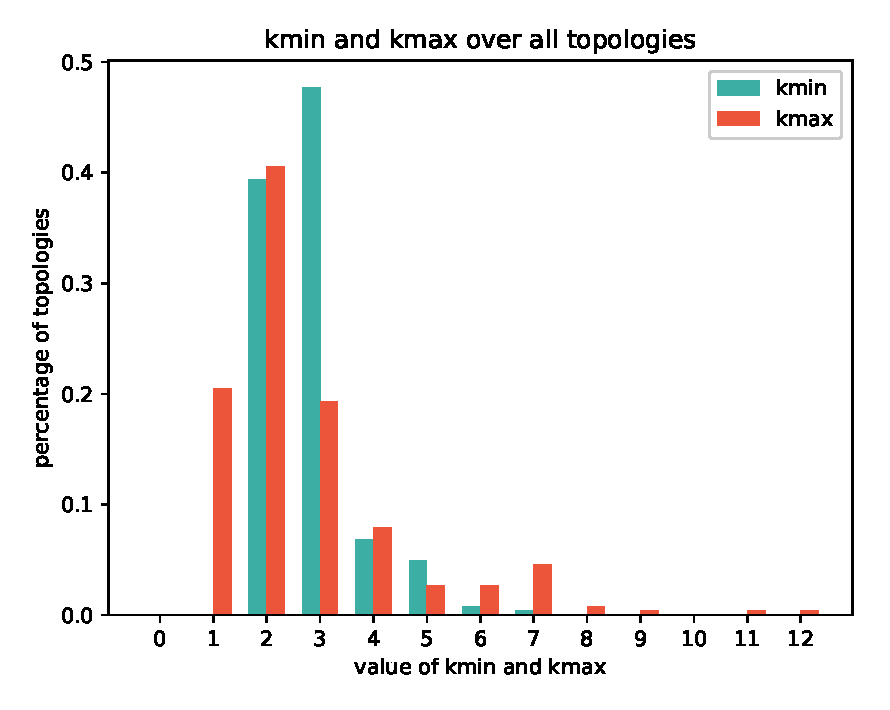
\includegraphics[width=.85\columnwidth]{./Network-lib/data/plot/kminkmax.eps}
\end{center}
\caption{Percentage of topologies for each given value of $\km(G)$ and $\kM(G)$.}
\label{fig:kminkmax}
\end{figure}

In the figure we observe that for $20\%$ of the instances, $\kM(G) = 1$. This means that with two segments, every node
can reach every other node with a deterministic sr-path. In other words, $20\%$ of the topologies do not contain ECMP which matches our analysis
of the topologies in Chapter \ref{chapter:dataset}. We also observe that in the worst case we need up to $12$ segments
to connect some pairs of nodes with a determinism sr-path. This value exceeds the capacity of most commercial routers but very few topologies
are in this case. For $90\%$ of the topologies, with at most $5$ segments any pair of routers can be connected with a deterministic sr-path.

We observe that for $87\%$ of the topologies, there exists some router on the network which is able to reach each other router with a deterministic
sr-path of segment cost at most $3$. We also see that we never need a sr-path path with segment cost larger than $7$ in order to find a root for a multi-cast tree implementable with segment routing.

These results are quite positive and indicate that path based solutions to networking optimization problems are likely to be
implementable with segment routing. This result is not a definitive answer as the measure that we would really like to compute in order to be able to answer these
questions is the maximum number of segments needed to represent any simple path in the original network. This would give an
upper bound on the number of segments required for implementing any path based solution with segment routing on each topology. 
Unfortunately computing this value is \NPhard~as we shown next.

%In this section we are going to study the problem of estimating the minimum number of
%segments required on a given network. We will start by showing that computing the 
%maximum number of segments required to minimaly segment any simple path in the network
%is \NPhard.

\begin{problem}{Maximum segmentation path}
\label{prob:max-seg}
Given a network $G$ compute the maximum value of $\cost(\mseg(p))$ such that $p$ is a simple path in $G$.
\end{problem}

In order to prove that Problem \ref{prob:max-seg} is \NPhard~ we need to defined some related problems first.
The first problem that we consider is the same except that we only focus on paths between two given nodes.

\begin{problem}{Maximum segmentation $s$-$t$ path}
\label{prob:max-seg-st}
Given a network $G$ and $s, t \in V(G)$ find a simple $s$-$t$ path $p$ such that $\cost(\mseg(p))$ is maximum.
\end{problem}


\begin{problem}{Unit weights longest path between nodes}
\label{prob:lpst}
Given a graph $G$ and $s, t \in V(G)$ compute the longest path from $s$ to $t$ in terms of the number of links
in the path.
\end{problem}

\begin{theorem}
Problem \ref{prob:lpst} is \NPhard. 
\end{theorem}

\begin{proof}
This is a known result. A proof can be found, for instance, in Corollary 8.11a from \cite{schrijver-book}.
\end{proof}

\begin{theorem}
\label{thm:max-seg-st-np}
Problem \ref{prob:max-seg-st} is \NPhard. 
\end{theorem}

\begin{proof}
We are going to prove that Problem \ref{prob:max-seg-st} is \NPhard by showing that
if we could solve it in polynomial time, then we could also solve Problem \ref{prob:lpst} in polynomial time.

Let $G, s, t$ be an instance of Problem \ref{prob:lpst}. Build a graph $H$ which is a copy of $G$ to which we add the following. For each
edge $(u, v) \in E(G)$, add a node $uv$ and two edges $(u, uv)$ and $(uv, v)$ both of weight $1$. Figure \ref{fig-np-max-seg}
illustrates this transformation.

\begin{figure}[H]
\begin{center}
\begin{tikzpicture}
\def\dx{0}
%\node[draw, circle, fill=lightgray] (a) at (\dx + 0, 0) {\tiny \texttt{a}};
%\node[draw, circle, fill=lightgray] (b) at (\dx + 1, 1) {\tiny \texttt{b}};
%\node[draw, circle, fill=lightgray] (c) at (\dx + 2, 2) {\tiny \texttt{c}};
%\node[draw, circle, fill=lightgray] (d) at (\dx + 3, 1) {\tiny \texttt{d}};
%\node[draw, circle, fill=lightgray] (e) at (\dx + 1, -1) {\tiny \texttt{e}};
%\node[draw, circle, fill=lightgray] (f) at (\dx + 3, -1) {\tiny \texttt{f}};

\node[scale=0.15] (a) at (\dx + -0.5, 0) {\router{a}{router}};
\node[scale=0.15] (b) at (\dx + 1, 1) {\router{b}{router}};
\node[scale=0.15] (c) at (\dx + 2, 2.3) {\router{c}{router}};
\node[scale=0.15] (d) at (\dx + 3, 1) {\router{d}{router}};
\node[scale=0.15] (e) at (\dx + 1, -1) {\router{e}{router}};
\node[scale=0.15] (f) at (\dx + 3, -1) {\router{f}{router}};


\draw[ultra thick] (a) -- (b);
\draw[ultra thick] (a) -- (e);
\draw[ultra thick] (b) -- (e);
\draw[ultra thick] (b) -- (c);
\draw[ultra thick] (c) -- (d);
\draw[ultra thick] (b) -- (d);
\draw[ultra thick] (b) -- (e);
\draw[ultra thick] (f) -- (d);
\draw[ultra thick] (f) -- (e);

\def\dx{6}
%\node[draw, circle, fill=lightgray] (a) at (\dx + 0, 0) {\tiny \texttt{a}};
%\node[draw, circle, fill=lightgray] (b) at (\dx + 1, 1) {\tiny \texttt{b}};
%\node[draw, circle, fill=lightgray] (c) at (\dx + 2, 2) {\tiny \texttt{c}};
%\node[draw, circle, fill=lightgray] (d) at (\dx + 3, 1) {\tiny \texttt{d}};
%\node[draw, circle, fill=lightgray] (e) at (\dx + 1, -1) {\tiny \texttt{e}};
%\node[draw, circle, fill=lightgray] (f) at (\dx + 3, -1) {\tiny \texttt{f}};


\node[scale=0.15] (a) at (\dx + -0.5, 0) {\router{a}{router}};
\node[scale=0.15] (b) at (\dx + 1, 1) {\router{b}{router}};
\node[scale=0.15] (c) at (\dx + 2, 2.3) {\router{c}{router}};
\node[scale=0.15] (d) at (\dx + 3, 1) {\router{d}{router}};
\node[scale=0.15] (e) at (\dx + 1, -1) {\router{e}{router}};
\node[scale=0.15] (f) at (\dx + 3, -1) {\router{f}{router}};

\draw[ultra thick] (a) -- (b);
\draw[ultra thick] (a) -- (e);
\draw[ultra thick] (b) -- (e);
\draw[ultra thick] (b) -- (c);
\draw[ultra thick] (c) -- (d);
\draw[ultra thick] (b) -- (d);
\draw[ultra thick] (b) -- (e);
\draw[ultra thick] (f) -- (d);
\draw[ultra thick] (f) -- (e);

\node[draw, fill=lightgray] (ab) at (\dx + 0, 1) {\tiny \texttt{ab}};
\draw[ultra thick, dotted] (a) edge[above, sloped] (ab);
\draw[ultra thick, dotted] (b) edge[above, sloped] (ab);

\node[draw, fill=lightgray] (ae) at (\dx + 0, -1) {\tiny \texttt{ae}};
\draw[ultra thick, dotted] (a) edge[below, sloped] (ae);
\draw[ultra thick, dotted] (e) edge[below, sloped] (ae);

\node[draw, fill=lightgray] (bc) at (\dx + 1, 2) {\tiny \texttt{bc}};
\draw[ultra thick, dotted] (bc) edge[below, sloped] (b);
\draw[ultra thick, dotted] (bc) edge[below, sloped] (c);

\node[draw, fill=lightgray] (cd) at (\dx + 3, 2) {\tiny \texttt{cd}};
\draw[ultra thick, dotted] (cd) edge[below, sloped] (c);
\draw[ultra thick, dotted] (cd) edge[below, sloped] (d);

\node[draw, fill=lightgray] (bd) at (\dx + 2, 0.5) {\tiny \texttt{bd}};
\draw[ultra thick, dotted] (bd) edge[sloped] (b);
\draw[ultra thick, dotted] (bd) edge[sloped] (d);

\node[draw, fill=lightgray] (be) at (\dx + 1.5, 0) {\tiny \texttt{be}};
\draw[ultra thick, dotted] (be) edge[sloped] (b);
\draw[ultra thick, dotted] (be) edge[sloped] (e);

\node[draw, fill=lightgray] (ef) at (\dx + 2, -0.5) {\tiny \texttt{ef}};
\draw[ultra thick, dotted] (ef) edge[sloped] (e);
\draw[ultra thick, dotted] (ef) edge[sloped] (f);

\node[draw, fill=lightgray] (df) at (\dx + 2.5, 0) {\tiny \texttt{df}};
\draw[ultra thick, dotted] (df) edge[sloped] (d);
\draw[ultra thick, dotted] (df) edge[sloped] (f);

\end{tikzpicture}
\end{center}
\caption{Example of the transformation. Solid edges have weight $2$ whereas dotted edges have weight $2$.}
\label{fig-np-max-seg}
\end{figure}

Let $p$ be a path on $H$ from $s$ to $t$ such that $\cost(\mseg(p))$ is maximum. We start by proving that $p$
does not cross any of the new nodes, that is, only crosses nodes in $V(G) \cap V(H)$. Suppose that $p$ visits the node
sequence $(v_1, \ldots, v_l)$ and let $i$ be the smallest index such that $v_i \notin V(G)$. Since $p$ is a path from
$s$ to $t$ and $s, t \in V(G)$ we have that $1 < i < l$. Thus we can write $v_i = v_{i-1}v_{i+1}$ and 
$p = (v_1, \ldots, v_{i - 1}, v_i, v_{i + 1}, \ldots, v_l) = (v_1, \ldots, v_{i - 1}, v_{i - 1} v_{i+1}, v_{i +1} \ldots, v_l)$.
We need to consider three cases.

\emph{Case 1:} $v_{i + 2} \in V(G)$. In this case path $p$ has the form:

\begin{center}
\begin{tikzpicture}[scale=0.8]
\node[scale=0.15] (v1) at (0, 0) {\router{$v_1$}{router}};
\node (dots) at (2, 0) {$\ldots$};
\node[scale=0.15] (vi-1) at (4, 0) {\router{$v_{i - 1}$}{router}};
\node[draw, fill=lightgray] (vi) at (6, 0) {\footnotesize $v_{i-1}v_{i+1}$};
\node[scale=0.15] (vi+1) at (8, 0) {\router{$v_{i + 1}$}{router}};
\node[scale=0.15] (vi+2) at (10, 0) {\router{$v_{i + 2}$}{router}};
\node (dots2) at (11, 0) {$\ldots$};

\draw (v1) edge[line width=2, ->] (dots);
\draw (dots) edge[line width=2, ->] (vi-1);
\draw (vi-1) edge[line width=2, dotted, ->] (vi);
\draw (vi) edge[line width=2, dotted, ->] (vi+1);
\draw (vi+1) edge[line width=2, ->] (vi+2);
\end{tikzpicture}
\end{center}

By construction, every link of $G$ that is traversed requires an adjacency segment
in its minimal segmentation (because of ECMP). 
Therefore, the minimal segmentation of this path is 
$$
\langle (v_1, v_2), (v_2, v_3), \ldots, (v_{i - 2}, v_{i - 1}), xy, (v_{i + 1}, v_{i + 2}), \ldots \rangle.
$$
On the other hand, if we remove element $xy$ from the path, we obtain a simple path $p'$ with the same minimal segmentation
except that $xy$ is replaced by the adjacency segment $(x, y)$ giving
$$
\langle (v_1, v_2), (v_2, v_3), \ldots, (v_{i - 2}, x), (x, y), (y, v_{i + 2}), \ldots \rangle.
$$
This segmentation costs one more than the segmentation of $p$. Since $p'$ is also a path from $s$ to $t$, this 
contradicts the fact that $p$ is a path from $s$ to $t$ that maximizes $\cost(\mseg(p))$.

\emph{Case 2:} $v_{i + 2} \notin V(G)$. In this case, $p$ has the following form:

\begin{center}
\begin{tikzpicture}[scale=0.8]
\node[scale=0.15] (v1) at (0, 0) {\router{$v_1$}{router}};
\node (dots) at (2, 0) {$\ldots$};
\node[scale=0.15] (vi-1) at (4, 0) {\router{$v_{i - 1}$}{router}};
\node[draw, fill=lightgray] (vi) at (6, 0) {\footnotesize xy};
\node[scale=0.15] (vi+1) at (8, 0) {\router{$v_{i + 1}$}{router}};
\node[draw, fill=lightgray] (vi+2) at (10, 0) {\footnotesize $v_{i + 2}$};
\node (dots2) at (11, 0) {$\ldots$};

\draw (v1) edge[line width=2, ->] (dots);
\draw (dots) edge[line width=2, ->] (vi-1);
\draw (vi-1) edge[line width=2, dotted, ->] (vi);
\draw (vi) edge[line width=2, dotted, ->] (vi+1);
\draw (vi+1) edge[line width=2, dotted, ->] (vi+2);
\end{tikzpicture}
\end{center}

The minimal segmentation of $p$ will be
$$
\langle (v_1, v_2), (v_2, v_3), \ldots, (v_{i - 2}, x), xy, v_{i + 2}, \ldots \rangle.
$$
As before, if we remove $xy$ from $p$ we obtain a simple path $p'$ from $s$ to $t$
with minimal segmentation equal to
$$
\langle (v_1, v_2), (v_2, v_3), \ldots, (v_{i - 2}, x), (x, y), v_{i + 2}, \ldots \rangle.
$$
This segmentation costs one more than the minimal segmentation of $p$ so as above, we conclude
that $p$ does not minimize $\cost(\mseg(p))$.

These two cases cover all possibilities so we conclude that the path $p$ on $H$ that maximizes
$\cost(\mseg(p))$ has all of its nodes in $V(G)$. Therefore, this is also a path in $G$.
Furthermore, because of ECMP, that the minimal segmentation of $p$ will contain
all of its edges as adjacency segments. Hence $\cost(\mseg(p)) = 2 |E(p)|$ so it follows that
if can find a path on $H$ that maximizes $\cost(\mseg(p))$ we can find a path on $G$ that maximizes
$E(p)$ which completes the proof.
% 
% 
% \newpage
% 
% Let $p = (v_1, v_2, \ldots, v_k)$ be a simple path in $G$. By theorem \todo{adjacency segment theorem}, each edge of path $p$
% requires an adjacency segment. Therefore, $\mseg(p) = \langle (v_1, v_2), (v_2, v_3), \ldots, (v_{k - 1}, v_k) \rangle$.
% 
% Let $p = (u_1, u_2, \ldots, u_k)$ be a path in $H$ such that $\cost(\mseg(p))$ is maximum. We are going to prove that
% there exists a path $q$ containing only nodes in $V(G)$ with the same segmentation cost.
% 
% 
% If $u_i \in V(G)$ for each $i = 1, \ldots, k$ then there is noting to prove. Othersiwe, let $i$ by the minimum index
% such that $u_i \notin V(G)$. Write $u_i = xy$ where $x, y \in V(G)$.
% 
% Then $p$ has the form $(u_1, \ldots, u_{i - 1}, u_i, u_{i + 1} \ldots) = (u_1, \ldots, x, xy, y, \ldots)$.
% The minimal segmentation of $p$ must has the form $\langle (u_1, u_2), (u_2, u_3), \ldots, (u_{i - 1}, x), \ldots, \rangle$
% 
% The minimal segmentation $\sr{p}$ of $p$ on $H$ is easy to characterize. 
% It will contain all special nodes $u_i \notin V(G)$ as node segments
% together with all edges $(u_i, u_{i + 1}) \in E(G)$ as adjacency segemnts (in their order of appearence). Finally,
% if $(u_1, u_2) \notin E(G)$ then $u_1$ will apprear as the first node and if $(u_{k - 1}, u_k) \notin E(G)$, then $u_k$
% will appear as the last node.
% 
% Therefore, if we remove the first special node $u_i \notin V(G)$ from $p$
% 
% \todo{STEPS:
% \begin{itemize}
%  \item Prove the structure of minimal segmentations on $H$
%  \item Prove that we can replace the first special node $ab$ by $b$. 
%  We need to make sure that the segment cost is not reduced and that we still have a simple path.
%  \item With this we show that there exists a solution of the problem that is a path in $G$.
%  \item We show that any path in $G$ maps to a path in $H$ with double segment cost.
%  \item We conclude that if there was a longer path in $G$ then we would have a longer segmentation
% \end{itemize}
% }
% 
% For instance, path $(a, ab, b, bc, c, d)$ has minimal segmentation $\langle a, ab, bc, (c, d) \rangle$.

\end{proof}

\begin{corollary}
Problem \ref{prob:max-seg} is \NPhard. 
\end{corollary}

\begin{proof}
Let $G, s, t$ be an instance of Problem \ref{prob:max-seg-st}. 
%We will build an instance $G'$ of Problem \ref{prob:max-seg}
%whose answer is the optimal solution of Problem \ref{prob:max-seg-st} plus some constant $C$. 
Let $m = E(G)$. We build a graph by adding a path $(x_1, \ldots, x_m, s)$ connecting to $s$ whose minimal segmentation 
has segment cost $2 m$ and a path $(t, y_1, \ldots, y_m)$ going out of $t$ whose minimal segmentation also has segment cost
$2 m$. This is achieved by adding also nodes $x'_1, \ldots, x'_m$ and $y'_1, \ldots, y'_m$ and edges $(x_i, x'_i)$ and
$(x'_i, x_{i + 1})$ of cost $1$ to ensure that adjacency segments are required to segment the two paths
mentioned above. Figure \ref{fig:np-transform2} illustrates this. Dashed edges represent edges of cost $1$
and solid edges represent edge of cost $2$.

\begin{figure}[H]
\begin{center}
\begin{tikzpicture}[scale=0.8]
\draw[ultra thick, lightgray, fill=lightgray!50!white] (0, 0) circle (2);
\node[scale=0.15] (s) at (-0.75, -0.75) {\router{$s$}{router}};
\node[scale=0.15] (t) at (0.75, 0.75) {\router{$t$}{router}};
\node[] (g) at (-1, 1) {$G$};

\node (gg) at (-5, 2) {$G'$};

\node[scale=0.15] (xm) at (-2.5, -0.75) {\router{$x_m$}{router}};
\node[scale=0.15] (xxm) at (-2.5, -3) {\router{$x'_m$}{router}};
\node[scale=0.15] (xm-1) at (-4.5, -0.75) {\router{$x_{m - 1}$}{router}};
\node[scale=0.15] (xxm-1) at (-4.5, -3) {\router{$x'_{m-1}$}{router}};
\node at (-5.5, -0.75) {$\ldots$};
\node[scale=0.15] (x1) at (-6.5, -0.75) {\router{$x_{1}$}{router}};
\node[scale=0.15] (xx1) at (-6.5, -3) {\router{$x'_{1}$}{router}};

\draw (xm) edge[line width=2, dotted, ->] (xxm);
\draw (xxm) edge[line width=2, dotted, ->] (s);
\draw (xm) edge[line width=2, ->] (s);

\draw (xm-1) edge[line width=2, dotted, ->] (xxm-1);
\draw (xxm-1) edge[line width=2, dotted, ->] (xm);
\draw (xm-1) edge[line width=2, ->] (xm);
\draw (x1) edge[line width=2, ->, dotted] (xx1);

\node[scale=0.15] (ym) at (2.5, 0.75) {\router{$y_m$}{router}};
\node[scale=0.15] (yym) at (2.5, 3) {\router{$y'_m$}{router}};
\node[scale=0.15] (ym-1) at (4.5, 0.75) {\router{$y_{m - 1}$}{router}};
\node[scale=0.15] (yym-1) at (4.5, 3) {\router{$y'_{m-1}$}{router}};
\node at (5.5, 0.75) {$\ldots$};
\node[scale=0.15] (y1) at (6.5, 0.75) {\router{$y_{1}$}{router}};
\node[scale=0.15] (yy1) at (6.5, 3) {\router{$y'_{1}$}{router}};


\draw (ym) edge[line width=2, dotted, <-] (yym);
\draw (yym) edge[line width=2, dotted, <-] (t);
\draw (ym) edge[line width=2, <-] (t);

\draw (ym-1) edge[line width=2, dotted, <-] (yym-1);
\draw (yym-1) edge[line width=2, dotted, <-] (ym);
\draw (ym-1) edge[line width=2, <-] (ym);
\draw (y1) edge[line width=2, <-, dotted] (yy1);

\draw[cyan, line width=2, ->] plot [smooth] coordinates { ($(x1)+(0,0.5)$) ($(xm-1)+(0,0.5)$) ($(xm)+(0,0.5)$)  ($(s)+(0,0.5)$) ($(s)+(0.5,0.5)$) ($(t)+(0,-0.5)$) ($(ym)+(0,-0.5)$) ($(ym-1)+(0,-0.5)$) ($(y1)+(0,-0.5)$)};



\end{tikzpicture}
\end{center}
\caption{Example of the transformation.}
\label{fig:np-transform2}
\end{figure}

By lemma \ref{lemma:edgeseg}, the maximum cost of a minimal segmentation in $G$ is at most $2 m$. Therefore,
the maximum cost of a minimal segmentation of a path in $G'$ must be a path from $x_1$ to $y_1$ since just this part
of the path will have segment cost at least $4m$. Since the path from $x_1$ passes by $s$, to each
$y_1$ we need to pass by $t$, we will achieve the maximum segment cost by connecting $s$ and $t$ by path with maximum 
segmentation cost. Thus the solution to Problem \ref{prob:max-seg} on $G'$ is a path of cost $x + 4m$ where $x$ is the cost of
the solution to problem \ref{prob:max-seg-st} on input $G, s, t$. We conclude that if we could solve Problem \ref{prob:max-seg}
in polynomial time then we could also solve Problem \ref{prob:max-seg-st} in polynomial time. Therefore, by Theorem \ref{thm:max-seg-st-np},
we conclude that \ref{prob:max-seg} is \NPhard.


\end{proof}



% ------------------------------------------------------------
% 
% \todo{this needs to be fixed, it still uses $\ereach(2, v)$ assuming that it mean unique shortest path}
% 
% \begin{theorem}
% \label{thm:ereach}
% Let $G$ be a network, $s \in V(G)$ and an integer $k \geq 3$. It holds that
% \begin{align*}
% \ereach(1, s) = & \ \emptyset \\
% \ereach(2, s) = & \ \{ e \in E(G) \mid \sp(s, v) \textrm{ is a path with last edge $e$} \} \quad \cup \\
%                 & \ \{ (s, u) \mid (s, u) \in E(G) \} \\
% \ereach(k, s) = & \ \bigcup_{v \in \nreach(k - 1, s)} \ereach(2, v) \quad \cup \\ 
% & \ \bigcup_{v \in \nreach(k - 2, s)}  \left\{ (u_1, u_2) \mid (u_1, u_2) \in E(G) \wedge u_1 \in \nreach(2, v) \right\}
% \end{align*}
% \end{theorem}
% 
% \begin{proof}
% For $k = 1$ the only sr-path of cost $1$ starting from $s$ is $\langle s \rangle$ and it contains no edges. Thus $\nreach(1, s) = \emptyset$.
% For $k = 2$, a sr-path of cost $2$ starting at $s$ has either the form $\langle s, v \rangle$ where
% $v \in V(G)$ or $\langle (s, v) \rangle$ where $(s, v) \in E(G)$. Thus, for each $v$ such that $\sp(s, v)$ is a path,
% the last edge will belong to $\ereach(2, s)$. Also, every edge of the form $(s, v)$ will belong to $\ereach(2, s)$
% 
% Let $k \geq 3$.
% 
% $(\subseteq)$ Let $e \in \ereach(k, v)$. Then there exists a deterministic sr-path 
% $\sr{p} = \langle x_1, \ldots, x_{l - 1}, x_l \rangle$  of segment cost at most $k$ such that
% either $x_l = e$ or $x_l$ is a node
% segment and $e$ is the last edge of the unique shortest path between $x^2_{l - 1}$
% and $x_{l}$. Let $\sr{q} = \langle x_1, \ldots x_{l - 1} \rangle$ and $v = x^2_{l - 1}$.
% 
% \emph{Case 1:} $x_l = e = (u_1, u_2)$. Let 
% Since $\cost(\sr{p}) \leq k$, we know that
% $\cost(\sr{q}) \leq k - 2$. Thus $v = x^2_{l - 1} \in \nreach(k - 2, s)$. 
% Since $\sr{p}$ is deterministic, 
% there must be a unique shortest path
% between $x^2_{l - 1} = v$ to $x^1_l = u_1$. Therefore, $u_1 \in \nreach(2, v)$ so
% $$
% e \in \bigcup_{v \in \nreach(k - 2, s)}  \left\{ (u_1, u_2) \mid (u_1, u_2) \in E(G) \wedge u_1 \in \nreach(2, v) \right\}.
% $$
% 
% \emph{Case 2:} $x_l$ is a node segment and $e$ is the last edge of the unique
% shortest path between $x^2_{l - 1}$ and $x_l$. Then $\cost(\sr{q}) \leq k - 1$
% so that $v \in \nreach(s, k - 1)$. Since $e$ is the last edge of the unique
% shortest path between $v = x^2_{l - 1}$ and $x_l$ we have that $e \in \ereach(2, v)$.
% Thus
% $$
% e \in \bigcup_{v \in \nreach(k - 1, s)} \ereach(2, v).
% $$
% 
% $(\supseteq)$ Let $e \in \bigcup_{v \in \nreach(k - 1, s)} \ereach(v, 2)$. Then
% there exists $v \in \nreach(k - 1, s)$ such that $e \in \ereach(v, 2)$. By definition,
% this means that there exists a deterministic sr-path $\sr{p} = \langle x_1, \ldots, x_l \rangle$
% from $s$ to $v$ with $\cost(\sr{p}) \leq k - 1$ and a unique shortest path from $v$ to $u$
% such that $e$ is the last edge of that path. Thus, $\langle x_1, \ldots, x_l, u \rangle$ is a deterministic
% sr-path from $s$ to $u$ of cost at most $k - 1 + 1 = k$ with last edge $e$. We conclude that
% $e \in \ereach(s, k)$.
% 
% Let $(u_1, u_2) \in \bigcup_{v \in \nreach(k - 2, s)}  \left\{ (u_1, u_2) \mid (u_1, u_2) \in E(G) \wedge u_1 \in \nreach(2, v) \right\}$.
% Then there exists $v \in \nreach(k - 2, s)$ such that $u_1 \in \nreach(2, v)$. 
% By definition, this means that we have a deterministic sr-path $\sr{p} = \langle x_1, \ldots, x_l \rangle$ from $s$ to $v$ with segment cost at most $k - 2$ and
% a unique shortest path from $v$ to $u_1$. Therefore $\langle x_1, \ldots, x_l, (u_1, u_2) \rangle$ is a deterministic sr-path
% from $s$ to $u_2$ of segment cost at most $k - 2 + 2 = k$ with last element being an adjacency segment
% on $(u_1, u_2)$. Hence, $(u_1, u_2) \in \ereach(k, s)$.
% \end{proof}


% \begin{proposition}
% Let $G$ be a network, $s \in V(G)$. Then for $k \geq 2$,
% \begin{align*}
% \nreach(0, s) = & \left\{ s \right\} \\
% \nreach(1, s) = & \left\{ V(\sp(s, v)) \mid \textrm{$v \in V(G)$ and $\sp(s, v)$ is a path} \right\} \\
% \nreach(k, s) = & \bigcup_{v \in \nreach(k - 1, s)} \nreach(1, v) \quad \cup \\
%                 & \left\{ u_2 \mid (u_1, u_2) \in E(G) \wedge \exists u \in \nreach(k - 2, s) : u_1 \in \nreach(1, u) \right\}
% \end{align*}
% \end{proposition}
% 
% \begin{proof}
% If $k = 0$ then the only sr-path starting at $s$ of segment cost at most $0$ is $\langle s \rangle$. Thus, since $V(\langle s \rangle) = s$, $\nreach(0, s) = \{ s \}$.
% For $k = 1$, the sr-paths starting at $s$ with segments cost at most $1$ are for the form $\langle s, v \rangle$ for $v \in V(G)$. From these, we only consider the ones
% that are deterministic, that is, the ones such that there is a unique shortest path between $s$ and $v$. In other words, the ones such that $\sp(s, v)$ is a path.
% 
% For $k \geq 2$ we will prove the that each set is contained inside the other. 
% 
% $(\subseteq)$ Let $v \in \nreach(k, s)$. Then, by definition, there exists a deterministic sr-path $\sr{p} = \langle x_1, \ldots, x_l \rangle$
% of cost at most $k$ such that $v \in V(\sr{p})$.
% \end{proof}




% \section{SR formalization}
% 
% In this section we propose a mathematical formalization of segment routing. This is a first step
% towards a uniformisation of the mathematical notations used to represent segments routing problems.
% 
% \todo{more blabla}
% 
% The first thing tht we are going to define are the concepts of node and adjacency segments.
% 
% \begin{definition}
% Let $G$ be a network. We define the \emph{segment set} of $G$ as $\seg(G) = V(G) \cup E(G)$.
% Let $x \in \seg(G)$. If $x = (u, v) \in E(G)$ we write $x^- = u$ and $x^+ = v$.
% Otherwise $x = v \in V(G)$ and we write $x^- = x^+ = v$.
% \end{definition}
% 
% Note that even for node segments we define the notations $x^-$ and $x^+$. As we will see shortly,
% it makes it possible to express other concept in a much more elegent maner as it avoids having
% to distinguish between the times of segments that are under consideration.
% 
% Next, we define the concept of segment routing paths, which essentially capture the segment
% stack that will be provided to the ingress node. The main difference between this definition and the
% ingress node is considered to be part of the path whereas in real netwoks it is not added to the SR stack.
% 
% \begin{definition}
% A \emph{segment routing path (sr-path)} is a sequence $\sr{p} = \langle x_1, \ldots, x_k \rangle$ such that each $x_i \in \seg(G)$ and
% for each $i = 2, \ldots k$, $x^+_{i - 1} \rightsquigarrow x^-_i$. We call $k$ the \emph{length} of $\sr{p}$ and write $\len(\sr{p}) = k$.
% 
% We write $\node(\sr{p}) = \{ x_i \mid x_i \in V(G) \}$ and call its elements \emph{node segments} and $\adj(\sr{p}) = \{ x_i \mid x_i \in E(G) \}$
% and call its elements \emph{adjacency segments}.
% 
% Finally, we define the \emph{segment cost} of $\sr{p}$ as $|\node(\sr{p})| + 2 \cdot |\adj(\sr{p})|$. We write it as $\cost(\sr{p})$.
% \end{definition}
% 
% The reason why adjacency segments have a double weight on the segment cost is because they require two entries in the segment
% stack instead of one. The segment cost is a huge constraint for SR as most routers have a very limited SR stack size \todo{ref}.
% 
% As we saw in the introduction, packets forwarded on a sr-path will follow shortest paths between consecutive segments. It can
% happen that more than one shortest path exists between to consecutive segments. This is called Equal-Cost MultiPath (ECMP) in the
% networking literature \todo{ref}. In this case, depending on the underlying
% application, one of two things can happend: (i) the traffic is split in some way among all those paths for load balancing or (ii)
% a single one of those paths is used to forward the traffic and this selection is done using a hash function. \todo{ref?} In the later case,
% the network operators have no way of knowing apriori which of them will be used.
% 
% In any case, we need a  way to describe all the network links that can contribute to the forwarding of packets between
% two consecutive segments. This leads to the definition of forwarding graphs.
% 
% \begin{definition}
% Let $\sr{p} = \langle x_1, \ldots, x_k \rangle$ be a sr-path. We define the \emph{forwarding graph} of $\sr{p}$ by
% $$
% \forw(\sr{p}) = \left( \bigcup_{i = 2}^k \sp(x^+_{i - 1}, x^-_{i}) \right) \cup \bigcup_{x \in \adj(\sr{p})} x.
% $$
% \end{definition}
% 
% The first part of the defintion of forwarding graphs captures all the shortest paths that are used between consecutive segments
% and the second part captures all links represented by adjacency segments. To better illustrate this defintion let's consider a few examples.
% 
% Figure \ref{fig:sr1} shows, in green, $\forw(\langle a, (d, e), i \rangle)$. To see that it matches the definition, we can write
% \begin{align*}
% \forw(\langle a, (d, e), i \rangle) & = \sp(a^+, (d, e)^-) \cup \sp( (d, e)^+, i^-) \cup (d, e) \\
% & = \sp(a, d) \cup \sp(e, i) \cup (d, e) \\
% & = (a, c, d) \cup (e, h, i) \cup (d, e) \\
% & = \{ (a, c), (c, d), (e, h), (h, i), (d, e) \}.
% \end{align*}
% 
% Consider now the sr-path $\sr{p} = \langle a, b, (d, e), i \rangle$ on the same graph as shown in Figure \ref{fig:sr2}. This
% example illustrates two things. First, from $b$ to the origin of $(d, e)$ there are two shortest paths so we see that
% $\forw(\sr{p})$ corresponds to a subgraph of $G$ and not just a path. Second, we see that the forwarding subgraph can
% contain cycles contrary to what our intuition might suggest. To confirm that this is correct we compute $\forw(\sr{p})$
% once more:
% \begin{align*}
% \forw(\langle a, b, (d, e), i \rangle) & = \sp(a^+, b^-) \cup \sp( b^+, (d, e)^-) \cup \sp( (d, e)^+, i^-) \cup (d, e) \\
% & = \sp(a, b) \cup \sp(b, e) \cup \sp(e, i) \cup (d, e) \\
% & = (a, b) \cup (b, c, d) \cup (b, e, d) \cup (e, h) \cup (h, i) \cup (d, e) \\
% & = \{ (a, b) (b, c), (c, d), (b, e), (e, d), (e, h), (h, i), (d, e) \}.
% \end{align*}
% 
% 
% \begin{figure}[H]
% \begin{center}
% \begin{tikzpicture}
% \def\x{0}
% \def\y{0}
% \node[scale=0.15] (a) at (0.5 + \x,  0.5 + \y) {\router{a}{green}};
% \node[scale=0.15] (b) at (0.5 + \x, -1.0 + \y) {\router{b}{green}};
% \node[scale=0.15] (c) at (2.5 + \x,  0.0 + \y) {\router{c}{lightgray}};
% \node[scale=0.15] (d) at (4.5 + \x,  0.0 + \y) {\router{d}{green}};
% \node[scale=0.15] (e) at (4.0 + \x, -2.0 + \y) {\router{e}{green}};
% \node[scale=0.15] (g) at (6.0 + \x,  0.5 + \y) {\router{g}{lightgray}};
% \node[scale=0.15] (i) at (8.0 + \x,  0.0 + \y) {\router{i}{green}};
% \node[scale=0.15] (h) at (7.0 + \x, -1.5 + \y) {\router{h}{lightgray}};
% \node[scale=0.15] (f) at (4.0 + \x, -3.5 + \y) {\router{f}{lightgray}};
% \node[scale=0.15] (j) at (8.0 + \x, -2.5 + \y) {\router{j}{lightgray}};
% \draw[line width=2] (f) edge[above, sloped] node[black,font=\bfseries] {\tiny \texttt{}} (j);
% \draw[line width=2] (h) edge[above, sloped] node[black,font=\bfseries] {\tiny \texttt{}} (j);
% \draw[line width=2] (a) edge[above, sloped] node[black,font=\bfseries] {\tiny \texttt{}} (b);
% \draw[line width=2] (b) edge[above, sloped] node[black,font=\bfseries] {\tiny \texttt{}} (c);
% \draw[line width=2] (e) edge[above, sloped] node[black,font=\bfseries] {\tiny \texttt{}} (c);
% \draw[line width=2] (b) edge[above, sloped] node[black,font=\bfseries] {\tiny \texttt{}} (e);
% \draw[line width=2] (b) edge[above, sloped] node[black,font=\bfseries] {\tiny \texttt{}} (f);
% \draw[line width=2] (e) edge[above, sloped] node[black,font=\bfseries] {\tiny \texttt{}} (f);
% \draw[line width=2] (h) edge[above, sloped] node[black,font=\bfseries] {\tiny \texttt{}} (f);
% \draw[line width=2] (g) edge[above, sloped] node[black,font=\bfseries] {\tiny \texttt{}} (i);
% \draw[line width=2] (i) edge[above, sloped] node[black,font=\bfseries] {\tiny \texttt{}} (h);
% \draw[line width=2]  (d) edge[above, sloped] node[black,font=\bfseries] {\tiny \texttt{}} (g);
% \draw[line width=2]  (d) edge[above, sloped] node[black,font=\bfseries] {\tiny \texttt{}} (e);
% \draw[line width=2]  (e) edge[above, sloped] node[black,font=\bfseries] {\tiny \texttt{}} (h);
% \draw[line width=2]  (g) edge[above, sloped] node[black,font=\bfseries] {\tiny \texttt{}} (h);
% \draw[line width=2]  (c) edge[above, sloped] node[black,font=\bfseries] {\tiny \texttt{}} (d);
% \draw[line width=2]  (a) edge[above, sloped] node[black,font=\bfseries] {\tiny \texttt{}} (b);
% \draw[line width=2]  (a) edge[above, sloped] node[black,font=\bfseries] {\tiny \texttt{}} (c);
% 
% %%%%
% \draw (a) edge[line width=2, darkgreen, above, ->, bend right = 20] (b);
% \draw (b) edge[line width=2, darkgreen, above, ->, bend left = 20] (c);
% \draw (b) edge[line width=2, darkgreen, above, ->, bend left = 20] (e);
% \draw (e) edge[line width=2, darkgreen, above, ->, bend left = 30] (d);
% \draw (c) edge[line width=2, darkgreen, above, ->, bend left = 20] (d);
% \draw (d) edge[line width=2, darkgreen, above, ->, dotted] (e);
% \draw (e) edge[line width=2, darkgreen, above, ->, bend left = 20] (h);
% \draw (h) edge[line width=2, darkgreen, above, ->, bend left = 20] (i);
% 
% 
% \def\x{-0.5}
% \def\y{1}
% \node at (\x + 2.7, \y + 0.25) {\footnotesize SR stack};
% \fill[lightgray] (\x, \y) rectangle (\x + 2, \y + 0.5);
% \fill[green] (\x, \y) rectangle (\x + 0.5, \y + 0.5);
% \draw[dotted, thick] (\x + 0.7, \y) -- (\x + 0.7, \y - 0.4);
% \draw[] (\x, \y) rectangle (\x + 2, \y + 0.5);
% \draw (\x + 0.5, \y) -- (\x + 0.5, \y + 0.5);
% \draw (\x + 1.5, \y) -- (\x + 1.5, \y + 0.5);
% \node at (\x + 0.25, \y + 0.26) {\footnotesize $b$};
% \node at (\x + 1, \y + 0.25) {\footnotesize $(d, e)$};
% \node at (\x + 1.75, \y + 0.28) {\footnotesize $i$};
% 
% 
% \def\x{-0.5}
% \def\y{-2}
% \fill[lightgray] (\x, \y) rectangle (\x + 2, \y + 0.5);
% \fill[gray] (\x, \y) rectangle (\x + 0.5, \y + 0.5);
% \fill[green] (\x + 0.5, \y) rectangle (\x + 1.5, \y + 0.5);
% \draw[dotted, thick] (\x + 0.7, \y + 0.5) -- (\x + 0.7, \y + 0.8);
% \draw[] (\x, \y) rectangle (\x + 2, \y + 0.5);
% \draw (\x + 0.5, \y) -- (\x + 0.5, \y + 0.5);
% \draw (\x + 1.5, \y) -- (\x + 1.5, \y + 0.5);
% \node at (\x + 0.25, \y + 0.26) {\footnotesize $b$};
% \node at (\x + 1, \y + 0.25) {\footnotesize $(d, e)$};
% \node at (\x + 1.75, \y + 0.28) {\footnotesize $i$};
% 
% 
% \def\x{3}
% \def\y{-3}
% \fill[lightgray] (\x, \y) rectangle (\x + 2, \y + 0.5);
% \fill[gray] (\x, \y) rectangle (\x + 1.5, \y + 0.5);
% \fill[green] (\x + 1.5, \y) rectangle (\x + 2, \y + 0.5);
% \draw[dotted, thick] (\x + 0.7, \y + 0.5) -- (\x + 0.7, \y + 0.8);
% \draw[] (\x, \y) rectangle (\x + 2, \y + 0.5);
% \draw (\x + 0.5, \y) -- (\x + 0.5, \y + 0.5);
% \draw (\x + 1.5, \y) -- (\x + 1.5, \y + 0.5);
% \node at (\x + 0.25, \y + 0.26) {\footnotesize $b$};
% \node at (\x + 1, \y + 0.25) {\footnotesize $(d, e)$};
% \node at (\x + 1.75, \y + 0.28) {\footnotesize $i$};
% 
% \def\x{8 - 0.75 - 0.25}
% \def\y{0.5}
% \fill[lightgray] (\x, \y) rectangle (\x + 2, \y + 0.5);
% \fill[gray] (\x, \y) rectangle (\x + 2, \y + 0.5);s
% \draw[dotted, thick] (\x + 0.7, \y) -- (\x + 0.7, \y - 0.4);
% \draw[] (\x, \y) rectangle (\x + 2, \y + 0.5);
% \draw (\x + 0.5, \y) -- (\x + 0.5, \y + 0.5);
% \draw (\x + 1.5, \y) -- (\x + 1.5, \y + 0.5);
% \node at (\x + 0.25, \y + 0.26) {\footnotesize $b$};
% \node at (\x + 1, \y + 0.25) {\footnotesize $(d, e)$};
% \node at (\x + 1.75, \y + 0.28) {\footnotesize $i$};
% 
% 
% %%%%
% 
% %\def\x{-1}
% 
% %\draw[line width=2] (\x + 10, \y + -1 + 0.5) edge[] (\x + 10.5, \y + -1 + 0.5);
% %\node[anchor=west]  at (\x + 10.5, \y + -1 + 0.5) {\footnotesize network link};
% 
% %\draw[line width=2] (\x + 10, \y + -1) edge[dotted, darkgreen, ->] (\x + 10.5, \y + -1);
% %\node[anchor=west]  at (\x + 10.5, \y + -1) {\footnotesize adjacency segment};
% 
% %\draw[line width=2] (\x + 10, \y + -1 - 0.5) edge[] (\x + 10.5, \y + -1 - 0.5);
% %\node[anchor=west]  at (\x + 10.5, \y + -1 - 0.5) {\footnotesize s link};
% 
% 
% \end{tikzpicture}
% \end{center}
% \label{fig:sr2}
% \caption{Illustration of SR with segments $b$, $(d, e)$ and $i$ and ingress node $a$. Dashed arrows represent adjacency segments
% and the others represent the shortest path edges between consecutive segments.}
% \end{figure}
% 
% Consider the path $p = (a, b, c, d)$. We have that both sr-paths $\sr{p} = \langle a, b, c, d \rangle$  and $\sr{q} = \langle c, d, a, b \rangle$ 
% satisfy $\forw(\sr{p}) = \forw(\sr{q}) = p$. However, only $\sr{p}$ respects the order of visited nodes of $p$ meaning that even though
% $\sr{q}$ is a segmentation of $q$, it does not faithfully represent $p$ from a traffic forwarding standpoint.
% 
% \begin{center}
% \begin{tikzpicture}
% \node[scale=0.15] (a) at (0, 0) {\router{a}{lightgray}};
% \node[scale=0.15] (b) at (2, 0) {\router{b}{lightgray}};
% \node[scale=0.15] (c) at (2, 2) {\router{c}{lightgray}};
% \node[scale=0.15] (d) at (0, 2) {\router{d}{lightgray}};
% 
% \draw[line width=2] (a) edge[above, sloped] node[black,font=\bfseries] {\tiny \texttt{}} (b);
% \draw[line width=2] (b) edge[above, sloped] node[black,font=\bfseries] {\tiny \texttt{}} (c);
% \draw[line width=2] (c) edge[above, sloped] node[black,font=\bfseries] {\tiny \texttt{}} (d);
% \draw[line width=2] (d) edge[above, sloped] node[black,font=\bfseries] {\tiny \texttt{}} (a);
% 
% \end{tikzpicture}
% \end{center}
% 


\section*{Conclusion}

In this chapter we provided a first formalization of segment routing that comprises both node and adjacency segments. 
We provided an algorithm for computing minimal segmentations. This algorithms opens the possibility of using traditional
graph algorithm for solving optimization problems over a network and then using it to segment and implement the solution on
a segment routed network. The advantage of this is that it allows to leverage the long lasting graph theory and
algorithms that have been developed without needing to extend those results to segment routing. The drawback of course
is that this approach yields no guarantees over the number of segments needed in the end. Maybe in the future, when the number
of segments in the segment stack becomes less of a limitation most solutions will eventually switch to this approach. However
for the time being, we still need solutions that take these constraints into account.

We also developed a reachability theory which constitutes the first steps towards having tools to analyze how well a network
is suited for segment routing. We will see in Chapter \ref{chapter:scmon} that this reachability theory makes it possible
to provide minimum segment cost cycle covers of a network in polynomial time.

\chapter{Optimal sr-paths}
\label{chapter:sr-optimal}

\section*{Introduction}

In this chapter we study several problems related to computing optimal sr-paths 
between two givens nodes. We start by defining weight functions for sr-paths and 
propose an algorithm for computing sr-paths of minimal weight with respect to such
a weight function and show how we can achieve low latency in a segment routed network. 
Next we study the reverse problem of finding a path of maximum
weight. Finally, we show how to compute sr-paths with maximum capacity. This is
useful to be able to route demands on a network without exceeding link capacities.

\section{Minimum weight sr-path}

The problem of computing minimum weight sr-paths appears 
in some form or another as a sub-problem in each of the three applications of segment routing
that we study in this thesis. It also has interesting applications in itself such as computing
sr-paths with minimum latency in the network or sr-paths with maximum bandwidth.

In order to be able to make sense of what we mean by a minimum weight sr-path, we need to define
weight functions for sr-paths which we call sr-metrics. These will essentially be generalizations of weight
function on graphs. To avoid confusion with minimum segment cost sr-paths, we will
always be careful to not interchange the words weight and cost. So whenever we mention the weight of a sr-path
we mean the value of some sr-metric when evaluated on that sr-path and whenever we mention its cost we are
thinking in terms of segments.

\begin{definition}
Let $G$ be a network. A \emph{sr-metric} is a function $w : \left( V(G) \times V(G) \right) \cup E(G) \rightarrow \mathbb{R} \cup \{ \infty \}$ such
that if there are no paths between $u$ and $v$ on $G$ then $w(u, v) = \infty$.
Given a sr-path $\sr{p} = \langle e_1, \ldots, e_n \rangle$ we define the weight $w(\sr{p})$ as
$$
w(\sr{p}) = \sum_{i = 2}^n w(x^2_{i - 1}, x^1_i) + \sum_{i : x_i \in E(G)} w(x_i).
$$
\end{definition}

The way to think about a sr-metric is that $w(u, v)$ for $u, v \in V(G)$ defines what we pay for traversing the shortest
paths between $u$ and $v$ and $w(e)$ for $e \in E(G)$ defines the weight of traversing edge $e$ with an adjacency segment.
The problem of finding minimum cost sr-paths with respect to some metric is defined as follows.

\begin{problem}{Minimum weight sr-path}
\label{problem:minweightsrpath}
\textbf{Input:} A network $G$, a sr-metric $w$, $k \in \mathbb{N}$ and two distinct nodes $s, t \in V(G)$.

\textbf{Output:} A sr-path $\sr{p} \in \mathcal{\sr{P}}_k(s, t)$ such that $w(\sr{p})$ is minimal.
\end{problem}

\subsection{General algorithm}

We propose in this section an algorithm for computing minimum weight sr-paths. The idea of this algorithm comes from
the Bellman-Ford shortest path algorithm \cite{Cormen:2009:IAT:1614191}. The Bellman-Ford algorithm is a dynamic programming (DP) algorithm
for computing shortest paths on graphs with both positive and negative edge weights from a given source $s$. At first sight, this might seem
totally different from what we are doing here. However if we look at the original dynamic programming formulation we see
that it is actually computing shortest paths of increasing lengths, in terms of edges. In a nutshell, they define DP
state spaces such that

\begin{align*}
\mathit{sol}(i, v) = \ & \textrm{the weight of the shortest path from} \\
            \ & \textrm{$s$ to $v$ using at most $i$ edges.}
\end{align*}

We are going to define a very similar state space in our solution. The main difference is that the
$i$ parameter will correspond the segment cost of the sr-path rather the a number of edges. We thus define the following DP state space

\begin{align*}
\mathit{sol}(i, v) = \ & \textrm{the minimum weight sr-path from} \\
            \ & \textrm{$s$ to $v$ with segment cost at most $i$.}
\end{align*}

The solution minimum weight sr-path problem is by definition $\mathit{sol}(k, t)$. For $i = 0$ the only possible sr-path of segment cost $0$ from $s$ to any node
is $\langle s \rangle$. Thus, we have that $\mathit{sol}(0, s) = 0$ and $\mathit{sol}(0, v) = \infty$ for $v \neq s$. 

The next step is to express $\mathit{sol}(i, *)$ in terms of $\mathit{sol}(j, s)$ with $j < i$.
The idea for doing this it to analyze the structure of a sr-path of cost $i$. There are three possibilities 
to reach a node $v$ with a sr-path of segment cost at most $i$.
These three possibilities are illustrated in Figure \ref{fig:dp}.
The first way is to simply not use
the extra segment and reach $v$ in the best way using a sr-path of segment cost at most
$i - 1$. The second possibility is to reach some node $u \in V$ using a sr-path of
segment cost at most $i - 1$ and then use one extra node segment to reach $v$ incurring an extra cost of $w(u, v)$. 
Finally, we can use a sr-path of cost at most $i - 2$ to any node $r$ and then append to it an adjacency
segment $(u, v)$ where $u$ is a in-neighbor of $v$. Note that nothing prevents $r$ from being equal to
$u$. In this case it simply means that we append the adjacency $(u, v)$ to a path that already ends at node
$u$. The cost increment of doing so is the cost of traversing the shortest path from $r$ to $u$ plus the cost
of the link $(u, v)$.

 \begin{figure}
 \begin{center}
 \begin{tikzpicture}
 \node[scale=0.15] (s) at (0, 0) {\router{s}{marked}};
 \node[scale=0.15] (x) at (5+2, 0) {\router{v}{marked}};
 \node[scale=0.15] (y) at (2+2, 0) {\router{u}{marked}};
 \node[scale=0.15] (z) at (4+2, -2) {\router{u}{marked}};
 \node[scale=0.15] (r) at (2+1, -2-0.2) {\router{r}{marked}};
 
 
 
 \draw (s) edge[very thick, below, bend right=10, dashed, ->] node {$\mathit{sol}(i - 1, v)$} (y);
 \draw (y) edge[very thick, bend right=10, dashed, ->, below] node {$w(u, v)$} (x);
 \draw (s) edge[very thick, bend left=40, dashed, ->, above] node {$\mathit{sol}(i - 1, v)$} (x);
 %\draw (s) edge[very thick, bend right=30, dashed, ->] (z);
 \draw (z) edge[very thick, ->, sloped, below] node {$w((u, v))$} (x);
 
 \draw (s) edge[very thick, bend right=30, dashed, ->, below, sloped] node {$\mathit{sol}(i - 2, r)$} (r);
 \draw (r) edge[very thick, bend right=20, dashed, ->, below, sloped] node {$w(r, u)$} (z);
 
 \end{tikzpicture}
 \end{center}
 \caption{Illustration of the $\mathit{sol}$ recurrence}
 \label{fig:dp}
 \end{figure}

The next theorem formalizes this intuition. 
 
\begin{theorem}
\label{thm:minwsrpath}
For $i \geq 1$ and $x \in V(G)$ it holds that

\small
\[\mathit{sol}(i, v) = \min \left\{
  \begin{matrix}
    \mathit{sol}(i - 1, v) &  \\[0.2cm]
    \mathit{sol}(i - 1, u)  +  w(u, v)  & s.t \text{ $y \in V$} \\[0.2cm]
    \mathit{sol}(i - 2, r)  +  w(r, u) + w((u, v)) & s.t \text{ $r \in V$} \\
\end{matrix}
  \right.
\]
\normalsize 
where the third value is only defined for $i \geq 2$ (set to $\infty$) otherwise.
\end{theorem}

\begin{proof}
Let $\sr{p} = \langle x_1, \ldots, x_n \rangle$ be a minimum weight sr-path from $s$ to $v$ of segment cost at most $i$. If 
$\cost(\sr{p}) < i$ then by definition $w(\sr{p}) = \mathit{sol}(i - 1, v)$. Suppose then
that $\cost(\sr{p}) = i$. We consider two cases.

\emph{Case 1: $x_n \in V(G)$}. In this case $\sr{q} = \langle x_1, \ldots, x_{n - 1} \rangle$ is a sr-path from $s$ to some node
$u = x^2_{n - 1}$ such that $w(\sr{q}) = i - 1$. It must be the case that $w(\sr{q}) = \mathit{sol}(i - 1, u)$ or otherwise 
we could replace it by a better sr-path and obtain a sr-path from $s$ to $v$ with lower weight. Therefore, by definition of $w$, we have
$$
\mathit{sol}(i, v) = w(\sr{p}) = w(\sr{q}) + w(u, v) = \mathit{sol}(i - 1, u) + w(u, v).
$$

\emph{Case 2: $x_n \in E(G)$}. This case is similar to the previous one. This time $\sr{q} = \langle x_1, \ldots, x_{n - 1} \rangle$ is a sr-path from $s$ to some node
$r = x^2_{n - 1}$ such that $w(\sr{q}) = i - 2$. Again, it must be the case that $w(\sr{q}) = \mathit{sol}(i - 2, r)$.
By definition of $w$, if we let $u = x^1_n$, it holds that
$$
\mathit{sol}(i, x) = w(\sr{p}) = w(\sr{q}) + w(x^2_{n - 1}, x^1_n) + w(x_n) = \mathit{sol}(i - 1, y) + w(r, u) + w((u, v)).
$$
\end{proof}

Since the values of $\mathit{sol}(i, *)$ depend only on $\mathit{sol}(i - 1, *)$, we can compute all these
values by iterating in increasing order of $i$. For each $i$, evaluating one state of the form
$(i, v)$ takes $O(|V(G)| + |V(G)| \cdot |\delta^-(v)|)$. Hence, given $i$, the cost of evaluating state $(i, v)$ 
all $v \in V(G)$ is $O(|V(G)|^2 + |V(G)| \cdot |E(G)|)$ making the total time complexity be $O(k \cdot |V(G)| \cdot |E(G)|)$.
A formalization of this algorithm is provided as Algorithm \ref{algo:min_weight_sr_path}.
Since this algorithm runs in polynomial time, we have the following result.

\begin{proposition}
Problem \ref{problem:minweightsrpath} can be solved in polynomial time. 
\end{proposition}

\begin{algorithm}[t]
\small
\caption{$\textsf{minWeightSrPath}\left( g, orig, dest, w, maxSeg \right)$}
\begin{algorithmic}[1]
\STATE $sol \gets \textsf{matrix}(maxSeg + 1, g.\textsf{V}(), \infty)$ \label{mwsrp-matrix}
\STATE $sol(0, orig) = 0$
\STATE $parent \gets \textsf{matrix}(maxSeg + 1, g.\textsf{V}(), \textbf{null})$
\FOR{$i = 1, \ldots, maxSeg$}
  \FOR{$cur \in g.\textsf{V}()$}
    \STATE $sol(i, cur) \gets sol(i - 1, cur)$
    \STATE $parent(i, cur) \gets parent(i - 1, cur)$
    \FOR{$prev \in g.\textsf{V}() \setminus \{ cur \}$} \label{mwsrp-for1}
      \IF{$sol(i - 1, prev) + w(prev, cur) < sol(i , cur)$} \label{mwsrp-if1}
        \cmtline{we reach $cur$ using node segment}
	\STATE $sol(i, cur) = sol(i - 1, prev) + w(prev, cur)$
	\STATE $parent(i, cur) \gets prev$
      \ENDIF
    \ENDFOR
    \cmtline{the third case is only defined for $i \geq 2$}
    \IF{$i \geq 2$}
      \FOR{$e = (orig, dest) \in g.\textsf{inEdges}(cur)$}
	\FOR{$prev \in g.\textsf{V}() \setminus \{ cur \}$} \label{mwsrp-for2}
	  \IF{$sol(i - 2, prev) + w(prev, orig) + w(e) < sol(i, cur)$} \label{mwsrp-if2}
	    \cmtline{we reach $cur$ using adjacency}
	    \STATE $sol(i, cur) = sol(i - 2, prev) + w(prev, orig) + w(e)$
	    \STATE $parent(i, cur) \gets e$
	  \ENDIF
	\ENDFOR
      \ENDFOR
    \ENDIF
  \ENDFOR
\ENDFOR
\STATE $opt \gets sol(maxSeg, dest)$
\STATE $k \gets maxSeg$
\WHILE{$k - 1 \geq 0 \textbf{ and } sol(k - 1, dest) = opt$}
  \STATE $k \gets k - 1$
\ENDWHILE
\RETURN $\textsf{SrPath}(parent, orig, dest, k, opt)$
\end{algorithmic}
\label{algo:min_weight_sr_path}
\end{algorithm}

% Bellman-Ford algorithm is known to admit an alternative implementation using a queue that makes it run much faster 
% in practice. This is know as the \emph{shortest path faster algorithm} (SPFA). Indeed, experiments show that the SPFA
% has a runtime comparable to Dijkstra's algorithm in practice. It has been proved that it worst case complexity is the same as
% the original Bellman-Ford algorithm but it is conjectured that its average run time is $O(|E|)$. No theoretical results have been proved to support this, only experimental
% ones. Motivated by this, we also provide an alternative implementaiton and evaluate it in practice to see
% how much time we can gain with with it.
% 
% The idea is that the for loops on lines \ref{mwsrp-for1} and \ref{mwsrp-for2} of Algorithm \ref{algo:min_weight_sr_path} makes some useless iterations.
% To see this, suppose that $sol(i, v) = sol(i - 1, v)$ for some $i$. Then, at iteration $i + 1$ it is useless to consider $prev = v$ on both these for loops.
% In order to avoid such iterations we will maintain a set of nodes $v$ for which $sol(i, v) < sol(i - 1, v)$ and only consider those nodes at iteration
% $i + 1$.

\subsection{Achieving minimum latency with SR}

In this section we explore the problem of computing and implementing minimum latency paths in a network.
In a typical network, routing is done using shortest path routing with respect to the IGP costs configured on the links.
These costs can be, to some extent, arbitrary and need not be related with the link latencies. This means that it can happen
that a suboptimal path is used for forwarding packets, with respect to the total time it takes the packets to travel from the 
origin to its destination. 

In Figure \ref{fig:minlat_example} we illustrate such an example in a real network. The IGP shortest path between routers
\node{a} and \node{c} is the one shown in the solid blue edges and has a total latency of $101.4$ milliseconds. On the other hand,
the path $(\node{a}, \node{d}, \node{e}, \node{c})$, represented by the green edges, only has a latency of $58.2$ milliseconds, that is,
it is 74\% faster. This path can be implemented with segment routing by adding, for instance, a detour towards router \node{d} before forwarding the traffic
to router \node{c}.

\begin{figure}
\begin{center}
\begin{tikzpicture}
\def\x{0}
\def\y{0}

\node[scale=0.15] (a) at (0 + \x,  0 + \y) {\router{a}{marked}};
\node[scale=0.15] (b) at (3 + \x,  0 + \y) {\router{b}{router}};
\node[scale=0.15] (c) at (6 + \x,  0 + \y) {\router{c}{marked}};
\node[scale=0.15] (d) at (0 + \x,  -2 + \y) {\router{d}{router}};
\node[scale=0.15] (e) at (6 + \x,  -2 + \y) {\router{e}{router}};

\draw[line width=2] (a) edge[above, sloped] node[black,font=\bfseries] {\footnotesize \texttt{975, 59.8}} (b);
\draw[line width=2] (b) edge[above, sloped] node[black,font=\bfseries] {\footnotesize \texttt{90, 41.6}} (c);
\draw[line width=2] (a) edge[above, sloped] node[black,font=\bfseries] {\footnotesize \texttt{5, 0.1}} (d);
\draw[line width=2] (d) edge[above, sloped] node[black,font=\bfseries] {\footnotesize \texttt{1001, 31.5}} (e);
\draw[line width=2] (e) edge[above, sloped] node[black,font=\bfseries] {\footnotesize \texttt{63, 26.6}} (c);

\node (a1) at (-1.3, -0.5) {};
\node (a2) at (-0.5, 1) {};

\node (b1) at (2.5, 1) {};
\node (b2) at (3.8, 0.9) {};

\node (c1) at (5.5, 1) {};
\node (c2) at (6.7, 0.7) {};
\node (c3) at (7.5, -0.5) {};

\node (e1) at (5.5, -1 - 2) {};
\node (e2) at (7.5, 0.5 - 2) {};

\node (d1) at (0.3, -3) {};


% \draw[line width=2] (a) edge[above, sloped] node[black,font=\bfseries] {\footnotesize \texttt{}} (a1);
% \draw[line width=2] (a) edge[above, sloped] node[black,font=\bfseries] {\footnotesize \texttt{}} (a2);
% \draw[line width=2] (d) edge[above, sloped] node[black,font=\bfseries] {\footnotesize \texttt{}} (d1);
% 
% \draw[line width=2] (b) edge[above, sloped] node[black,font=\bfseries] {\footnotesize \texttt{}} (b1);
% \draw[line width=2] (b) edge[above, sloped] node[black,font=\bfseries] {\footnotesize \texttt{}} (b2);
% 
% \draw[line width=2] (c) edge[above, sloped] node[black,font=\bfseries] {\footnotesize \texttt{}} (c1);
% \draw[line width=2] (c) edge[above, sloped] node[black,font=\bfseries] {\footnotesize \texttt{}} (c2);
% \draw[line width=2] (c) edge[above, sloped] node[black,font=\bfseries] {\footnotesize \texttt{}} (c3);
% 
% \draw[line width=2] (e) edge[above, sloped] node[black,font=\bfseries] {\footnotesize \texttt{}} (e1);
% \draw[line width=2] (e) edge[above, sloped] node[black,font=\bfseries] {\footnotesize \texttt{}} (e2);


\draw (a) edge[line width=2, cyan, above, ->, bend right = 20] (b);
\draw (b) edge[line width=2, cyan, above, ->, bend right = 20] (c);

\draw (a) edge[line width=2, seagreen, above, ->, bend right = 20] (d);
\draw (d) edge[line width=2, seagreen, above, ->, bend right = 10] (e);
\draw (e) edge[line width=2, seagreen, above, ->, bend right = 20] (c);

\draw (8, -1) edge[line width=2, above] node {$\igp, \lat$} (9, -1);

\end{tikzpicture}
\end{center}
\caption{A small subgraph of a real network where the IGP shortest path between two nodes paths is 74\% slower than the optimal path.}
\label{fig:minlat_example}
\end{figure}

Although this example shows that SR can sometimes make it possible to find much more efficient paths, our
experiments show that the average gain is actually much lower than the 74\% shown above and that this is
an outlier result. For every topology in our data set,
we computed for every pair of distinct nodes, the minimum latency path between them and computed the ratio
between this value and the latency of the IGP shortest path. Figure \ref{fig:minlat_box} shows a box plot of these ratios.
On the $x$-axis, we either have a single topology or a topology group, and on the $y$-axis we have the ratio between
the nominal latency (latency of the IGP shortest path) and minimum latency of any path connecting the same
origin and destination.
We aggregated the results for the Zoo topologies because this data set contains over
200 topologies making it impossible show all of them. The last box shows the aggregated results over all topologies.
We can observe that the average gain is only 8\%, much lower than our example.

However, it is still interesting to study the problem of finding minimum latency segment routing paths for two reasons.
First, even if the gain is not as significant as our above example on average, there is still something to be gained in terms 
of latency when using SR over IGP shortest path routing as the overhead of doing so is quite small since
SR does not require routers to maintain state.
Second, as we will see later, this problem appears in some form or another as a subproblem of other
problems that we have tackled in this thesis.

\begin{figure}
\begin{center}
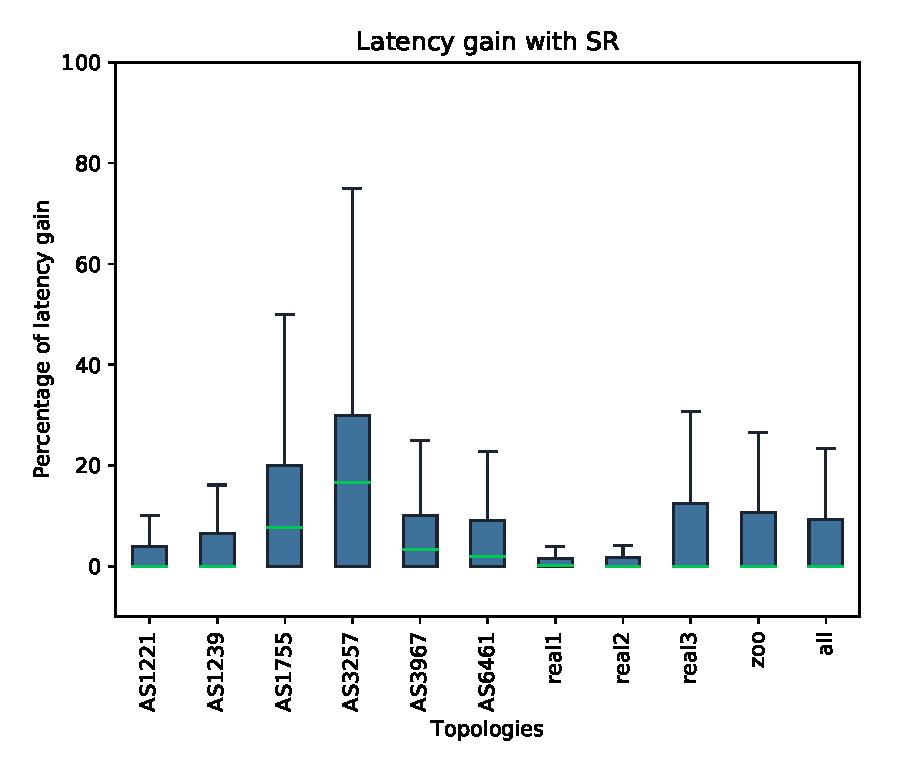
\includegraphics[scale=0.6]{./Network-lib/data/plot/minLat.eps}
\end{center}
\caption{Latecy gain in percentage.}
\label{fig:minlat_box}
\end{figure}

\subsubsection{Shortest path plus segmentation}

The first way to solve this problem with segment routing is to simply use a shortest path algorithm such as Dijkstra's algorithm
to compute the minimum latency path between the origin and the destination. Then, in order to implement that path with segment routing,
we can use the minimal segmentation algorithm proposed in Chapter \ref{chapter:sr} to segment that path.

The problem with doing this is that we have no control over the number of segments in the final path. If could be the case that the
minimum latency path actually requires a huge amount of segments to be implemented. Figure \ref{fig:minlat_seg} shows the distribution of
the number of segments required in the segmentation of the minimum latency paths over all pairs of nodes in the topologies from
our data set.

\begin{figure}
\begin{center}
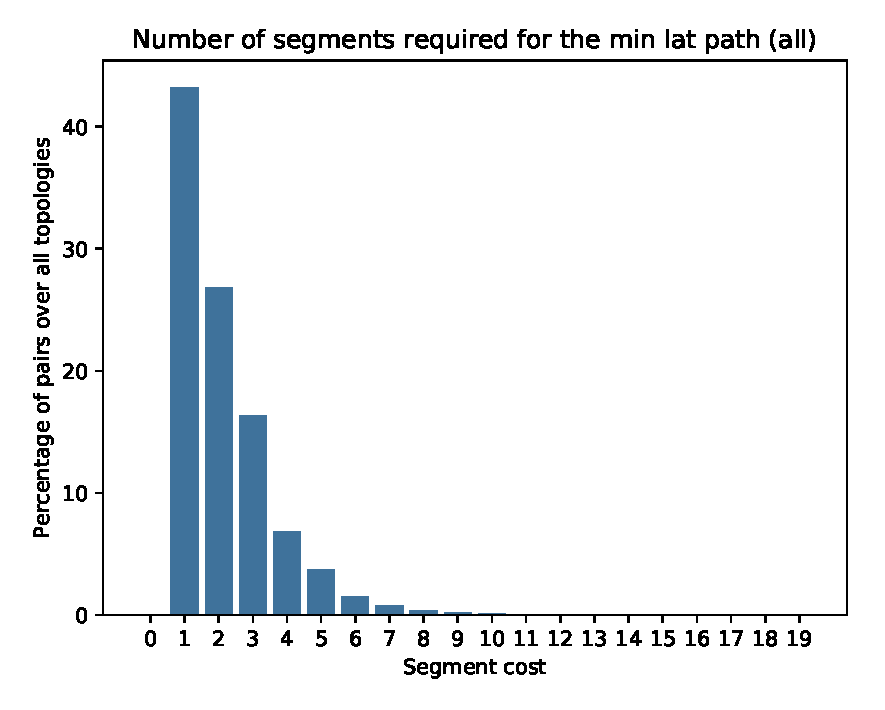
\includegraphics[scale=0.6]{./Network-lib/data/plot/minLat_seg.eps}
\end{center}
\caption{Number of segments required in the minimum latency paths over all topologies.}
\label{fig:minlat_seg}
\end{figure}

These results indicate that on average, there is some correlation between the IGP shortest paths and the
minimum latency paths. For $20$\% of the pairs over all topologies, the IGP shortest path matches the minimum latency
path. With about $5$ segments we can already route over $96$\% of the minimum latency paths. Thus we can say
that on average computing the minimum latency path and then segmenting it will yield a path that requires a small
segment stack and this is likely to be implementable on the network.

However, there are some topologies where this is far from true. Figure \ref{fig:minlat_seg_ovh} shows the same results
but for a single topology \topo{OVH-EUR}.

\begin{figure}
\begin{center}
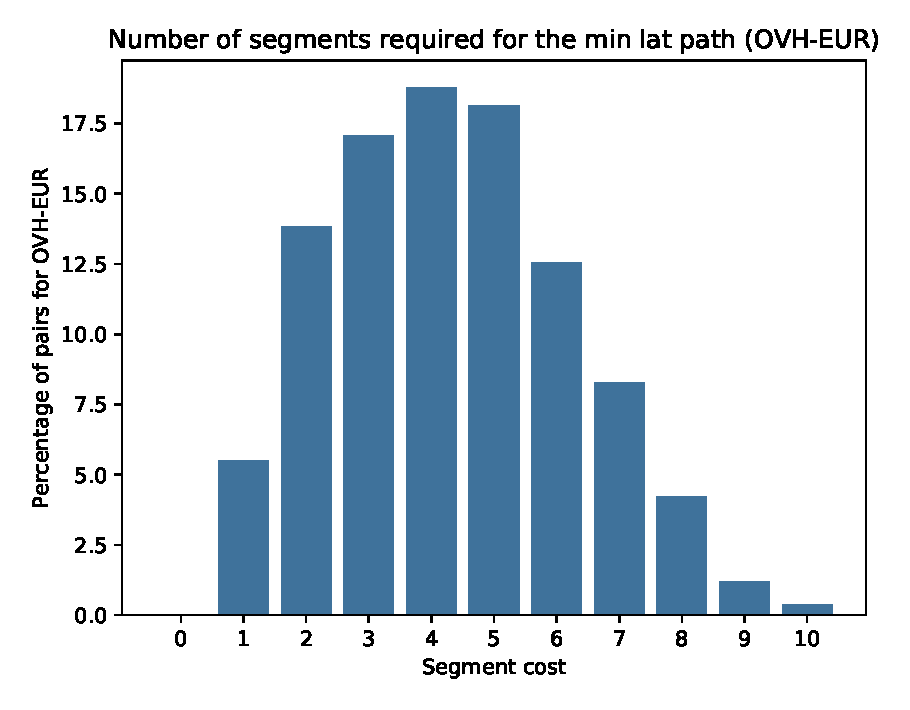
\includegraphics[scale=0.6]{./Network-lib/data/plot/minLat_seg_ovh.eps}
\end{center}
\caption{Number of segments required in the minimum latency paths for \topo{OVH-EUR}.}
\label{fig:minlat_seg_ovh}
\end{figure}

For this topology the situation is quite different as we need more than $5$ segments for about $26$\% of the pairs.
The reason why we observe this behavior in the \topo{OVH-EUR} topology is because it contains a lot of link
bundles having parallel links. This creates a lot of ECMP making it hard for segment routing to pass by
very specific paths.

This motivates the need for a minimum latency path finding algorithm that takes into account the number of 
segments from the start rather than simply computing a minimum latency path and hope that by chance it will
not requite a long segment stack.

%\todo{Talk about the case of equal cost latency. In this case maybe there is a path with less segments and equal latency.
%This is a bit technical, need to find a good way to talk about this.}

\subsubsection{Minimum latency SR-Path problem}

Another way of approaching this problem is to define a suitable sr-metric and use Algorithm \ref{algo:min_weight_sr_path} for computing a minimum 
latency sr-path. In this way
we will have full control over the number of segments in the output. The price to pay with this is that the latency of the obtained sr-path
will not be the global minimum but only the local minimum over all sr-paths in $\mathcal{\sr{P}}_k$.

To be able to define the problem more formally we need to define what is the latency of a sr-path.
This might seem obvious but in the presence of ECMP, a sr-path will correspond to a subnetwork of the original
network rather than a simple path. In reality, as we mentioned previously, the behavior of the network may vary making it impossible to
know which path amongst all paths defined by the sr-path will actually be used to forward traffic.

Let us illustrate this in a real example. Figure \ref{fig:spdag_ecmp} shows the shortest path subnetwork between routers \node{a} and \node{j} in a real network.
Both paths have the same IGP cost of $72$. The top path has latency $25.36ms$ and the bottom one has $19.1ms$.
Whenever we have a sr-path of the form $\langle \ldots, \node{a}, \node{j}, \ldots \rangle$, we do not know whether path $(\node{a}, \node{b}, \node{d}, \node{f}, \node{j})$ or $(\node{a}, \node{c}, \node{e}, \node{g}, \node{h}, \node{i}, \node{j})$
will be used to forward traffic between \node{a} and \node{j}.

\begin{figure}
\begin{center}
\begin{tikzpicture}
\def\x{0}
\def\y{0}

\node[scale=0.15] (a) at (0 + \x,  0 + \y) {\router{a}{marked}};
\node[scale=0.15] (b) at (0 + \x,  2 + \y) {\router{b}{router}};
\node[scale=0.15] (c) at (0 + \x,  -2 + \y) {\router{c}{router}};
\node[scale=0.15] (d) at (2.5 + \x,  2 + \y) {\router{d}{router}};
\node[scale=0.15] (e) at (2.5 + \x,  -2 + \y) {\router{e}{router}};
\node[scale=0.15] (f) at (5 + \x,  2 + \y) {\router{f}{router}};
\node[scale=0.15] (g) at (5 + \x,  -2 + \y) {\router{g}{router}};
\node[scale=0.15] (h) at (7.5 + \x,  -2 + \y) {\router{h}{router}};
\node[scale=0.15] (i) at (10 + \x,  -2 + \y) {\router{i}{router}};
\node[scale=0.15] (j) at (10 + \x,  2 + \y) {\router{j}{marked}};


\draw[line width=2] (a) edge[above, sloped, ->] node[black,font=\bfseries] {\footnotesize \texttt{41, 19.5}} (b);
\draw[line width=2] (b) edge[above, sloped, ->] node[black,font=\bfseries] {\footnotesize \texttt{25, 5.5}} (d);
\draw[line width=2] (d) edge[above, sloped, ->] node[black,font=\bfseries] {\footnotesize \texttt{1, 0.1}} (f);
\draw[line width=2] (f) edge[above, sloped, ->] node[black,font=\bfseries] {\footnotesize \texttt{5, 0.26}} (j);

\draw[line width=2] (a) edge[below, sloped, ->] node[black,font=\bfseries] {\footnotesize \texttt{1, 0.1}} (c);
\draw[line width=2] (c) edge[above, sloped, ->] node[black,font=\bfseries] {\footnotesize \texttt{38, 4.8}} (e);
\draw[line width=2] (e) edge[above, sloped, ->] node[black,font=\bfseries] {\footnotesize \texttt{1, 0.1}} (g);
\draw[line width=2] (g) edge[above, sloped, ->] node[black,font=\bfseries] {\footnotesize \texttt{30, 13.9}} (h);
\draw[line width=2] (h) edge[above, sloped, ->] node[black,font=\bfseries] {\footnotesize \texttt{1, 0.1}} (i);
\draw[line width=2] (i) edge[above, sloped, ->] node[black,font=\bfseries] {\footnotesize \texttt{1, 0.1}} (j);

\node (a1) at (-1.3, -0.5) {};
\node (a2) at (-0.5, 1) {};

\node (b1) at (2.5, 1) {};
\node (b2) at (3.8, 0.9) {};

\node (c1) at (5.5, 1) {};
\node (c2) at (6.7, 0.7) {};
\node (c3) at (7.5, -0.5) {};

\node (e1) at (5.5, -1 - 2) {};
\node (e2) at (7.5, 0.5 - 2) {};

\node (d1) at (0.3, -3) {};


\draw (8, -3.5) edge[line width=2, above] node {$\igp, \lat$} (9, -3.5);


% \draw[line width=2] (a) edge[above, sloped] node[black,font=\bfseries] {\footnotesize \texttt{}} (a1);
% \draw[line width=2] (a) edge[above, sloped] node[black,font=\bfseries] {\footnotesize \texttt{}} (a2);
% \draw[line width=2] (d) edge[above, sloped] node[black,font=\bfseries] {\footnotesize \texttt{}} (d1);
% 
% \draw[line width=2] (b) edge[above, sloped] node[black,font=\bfseries] {\footnotesize \texttt{}} (b1);
% \draw[line width=2] (b) edge[above, sloped] node[black,font=\bfseries] {\footnotesize \texttt{}} (b2);
% 
% \draw[line width=2] (c) edge[above, sloped] node[black,font=\bfseries] {\footnotesize \texttt{}} (c1);
% \draw[line width=2] (c) edge[above, sloped] node[black,font=\bfseries] {\footnotesize \texttt{}} (c2);
% \draw[line width=2] (c) edge[above, sloped] node[black,font=\bfseries] {\footnotesize \texttt{}} (c3);
% 
% \draw[line width=2] (e) edge[above, sloped] node[black,font=\bfseries] {\footnotesize \texttt{}} (e1);
% \draw[line width=2] (e) edge[above, sloped] node[black,font=\bfseries] {\footnotesize \texttt{}} (e2);
% 
% 
% \draw (a) edge[line width=2, cyan, above, ->, bend right = 20] (b);
% \draw (b) edge[line width=2, cyan, above, ->, bend right = 20] (c);
% 
% \draw (a) edge[line width=2, seagreen, above, ->, bend right = 20, dotted] (d);
% \draw (d) edge[line width=2, seagreen, above, ->, bend right = 10, dotted] (e);
% \draw (e) edge[line width=2, seagreen, above, ->, bend right = 20, dotted] (c);


\end{tikzpicture}
\end{center}
\caption{The shortest path DAG between routers \node{a} and \node{j} in a real network.}
\label{fig:spdag_ecmp}
\end{figure}

If we want to be able to provide guarantees about the latency, we need to consider the worst case scenario where, whenever
there is more than one path, we assume the slowest one is used. This corresponds to defining the latency of a sr-path
$\langle s_1, s_2 \rangle$ as the \emph{longest path} (w.r.t latencies) of any paths between $s_1$ and $s_2$ on $\sp(s_1, s_2)$.
This motivates the following definition.

\begin{definition}
Let $s_1, s_2$ be two nodes of a network $G$ and $e$ an edge.
The \emph{maximum latency sr-metric} is defined as
$$
\latmax(s_1, s_2) = \textrm{maximum latency of a path from $s_1$ to $s_2$ in $\sp(s_1, s_2)$}
$$
and
$$
\latmax(e) = \lat(e).
$$
\end{definition}

With this metric, we have $\latmax(\node{a}, \node{j}) = 25.38$. Note that on single edges this metric is defined as to
match that edge's latency. It is important to notice that this metric can be computed efficiently. It is well known that the
longest path problem is \textsf{NP}-hard in general \cite{Cormen:2009:IAT:1614191}. However, in this case we are computing it on an
acyclic network (the shortest path subnetwork) which can be done in linear time with a simple dynamic programming algorithm \cite{Cormen:2009:IAT:1614191}.

Another metric that is of interest is to consider that the latency of a sr-path is the average latency over all shortest paths.
This corresponds in practice with a situation where the next hops are selected randomly in case of ECMP. It somehow
reflects the behavior of selecting the next hops with an unknown hash function when several possible next hops exist.

\begin{definition}
Let $s_1, s_2$ be two nodes of a network $G$ and $e$ an edge.
The \emph{average latency sr-metric} is defined as
$$
\latavg(s_1, s_2) = \textrm{average latency among all paths from $s_1$ to $s_2$ in $\sp(s_1, s_2)$} 
$$
and
$$
\latavg(e) = \lat(e).
$$
\end{definition}

This metric can also be computed efficiently. We can use dynamic programming to compute the number of paths and their total
cost in linear time. The only complication is that this number grows exponentially which can easily be overcome using 
arbitrary precision integers.

Figure \ref{fig:ecmp_pc} shows the distribution of the number of equal cost shortest path between all pairs of routers over
all topologies. We can see about $60$\% of the time there is a single shortest path between the pairs of nodes. 
The maximum number of paths found for any pair of nodes was $11150$. This value might seem huge but it is actually quite small
when we take into the fact the number of paths in a DAG can be as large as $2^{|V| - 2}$ where $|V|$ is the number of routers in
that topology. This means that when computing average measures, we can probably use normal integers rather than arbitrary precision integers.

\begin{figure}
\begin{center}
\includegraphics[scale=0.6]{./Network-lib/data/plot/ecmpPathCount.eps}
\end{center}
\caption{Evaluation of the average number of ECMP over all topologies.}
\label{fig:ecmp_pc}
\end{figure}

\section{Maximum weight sr-paths}

In this section, we briefly discuss the problem of finding maximum weight sr-paths. 

\begin{problem}{Maximum weight sr-path}
\label{problem:maxweightsrpath}
\textbf{Input:} A network $G$, a sr-metric $w$, an integer constant $k \geq 1$ and two distinct nodes $s, t \in V(G)$.

\textbf{Output:} A sr-path $\sr{p} \in \mathcal{\sr{P}}_k(s, t)$ such that $w(\sr{p})$ is maximal.
\end{problem}

This problem can be solved in the exact same way as the minimum weight sr-path problem (Problem \ref{problem:minweightsrpath})
by replacing the $\infty$ by $-\infty$ on line \ref{mwsrp-matrix} and replacing the $<$ by $>$ on lines \ref{mwsrp-if1} and
\ref{mwsrp-if2} of Algorithm \ref{algo:min_weight_sr_path}.

This result might seem unintuitive at first because, as mentioned at the end of Chapter \ref{chapter:sr}, the longest path problem on graphs is \NPhard. Hence,
one might think by setting $k$ arbitrarily high and by using an appropriate sr-metric the two problems could become the same. There
is however an important nuance. In this problem we are not preventing the sr-path from repeating segments while the longest path
problem required simple paths. It is not hard to see that if we drop the simple path constraint then the longest path problem becomes trivial:
if the input graph is acyclic then we compute the answer with dynamic programming otherwise the answer is $\infty$ since we can
traverse any cycle an arbitrary amount of times getting longer and longer paths.

The next question one might then ask about this problem is, can this problem be interesting for some sr-metric $w$? The answer
is yes as we will see in Chapter \ref{chapter:scmon}.

\section{Maximum capacity sr-paths}

When routing traffic over a network it can be the case that the network is highly loaded. This can cause some network links
to become congested such as for instance, shortest path links or the links in the minimum latency path. Motivated by this,
we study the problem of finding a sr-path between two nodes whose congestion in minimum. Having such an algorithm can be
an interesting building block for dynamically allocating incoming demands while doing a best effort to prevent congestion.
Of course, using such an algorithm locally for each incoming demand will lead to an overall sub-optimal solution. We will
study the problem of considering all demands at once on Chapter \ref{chapter:te}.

We start with a very simple definition of demand.

\begin{definition}
A \emph{demand} in a network $G$ is a triple $(s, t, \nu)$ where $s, t \in V(G)$ and $\nu \in \mathbb{N}^+$. Given a demand $d$
we write $\src(d) = s$, $\dst(d) = t$ and $\vol(d) = \nu$.
\end{definition}

Before formally defining the problem that we solve in this section, we need to understand how traffic on a sr-path affects 
link loads since sr-paths can actually correspond to
several paths on the original network in case of ECMP. In this section we assume that the network is using a traffic split 
mechanism. Recall that this means that in the presence of ECMP,
the routers evenly split the incoming traffic amongst those equal cost paths. Consider sending one unit of flow
from node \node{a} to node \node{d} on the graph shown in Figure \ref{fig:split-example}. There are two shortest
paths between these nodes: $((\node{a}, \node{c}), (\node{c}, \node{d}))$ and $((\node{a}, \node{b}), (\node{b}, \node{d}))$.
Therefore, there will be a 50-50 split of the load over these two paths.

\begin{figure}[H]
\begin{center}
\begin{tikzpicture}[scale=1.2]
%\node[draw, circle] (a) at (0, 0) {\tiny \texttt{a}};

\node[scale=0.15] (a) at (0, 0)     {\router{a}{marked}};
\node[scale=0.15] (b) at (1, -1)    {\router{b}{router}};
\node[scale=0.15] (c) at (1, 1)     {\router{c}{router}};
\node[scale=0.15] (d) at (3, -1)    {\router{d}{marked}};
\node[scale=0.15] (e) at (3.5, 1.5) {\router{e}{router}};
\node[scale=0.15] (f) at (3.5, 0)   {\router{f}{router}};
\node[scale=0.15] (g) at (5, 1)     {\router{g}{router}};
\node[scale=0.15] (h) at (5, -1)    {\router{h}{router}};
\node[scale=0.15] (i) at (6, 0)     {\router{i}{router}};
\node[scale=0.15] (j) at (7.5, 0.5) {\router{j}{router}};
\node[scale=0.15] (k) at (7.5, -1)  {\router{k}{router}};

\draw[line width=2] (a) edge[above, sloped] node[black,font=\bfseries] {\footnotesize \texttt{$50\%$}} (c);
\draw[line width=2] (c) edge[above, sloped] node[black,font=\bfseries] {\footnotesize \texttt{$50\%$}} (d);
\draw[line width=2] (a) edge[above, sloped] node[black,font=\bfseries] {\footnotesize \texttt{$50\%$}} (b);
\draw[line width=2] (b) edge[above, sloped] node[black,font=\bfseries] {\footnotesize \texttt{$50\%$}} (d);


\draw[line width=2] (c) edge[above, sloped] node[black,font=\bfseries] {\footnotesize \texttt{}} (e);
\draw[line width=2] (c) edge[above, sloped] node[black,font=\bfseries] {\footnotesize \texttt{}} (f);
\draw[line width=2] (c) edge[above, sloped] node[black,font=\bfseries] {\footnotesize \texttt{}} (d);
\draw[line width=2] (e) edge[above, sloped] node[black,font=\bfseries] {\footnotesize \texttt{}} (g);
\draw[line width=2] (f) edge[above, sloped] node[black,font=\bfseries] {\footnotesize \texttt{}} (g);
\draw[line width=2] (f) edge[above, sloped] node[black,font=\bfseries] {\footnotesize \texttt{}} (h);
\draw[line width=2] (d) edge[above, sloped] node[black,font=\bfseries] {\footnotesize \texttt{}} (h);
\draw[line width=2] (g) edge[above, sloped] node[black,font=\bfseries] {\footnotesize \texttt{}} (i);
\draw[line width=2] (h) edge[above, sloped] node[black,font=\bfseries] {\footnotesize \texttt{}} (i);
\draw[line width=2] (i) edge[above, sloped] node[black,font=\bfseries] {\footnotesize \texttt{}} (j);


\draw[line width=2] (a) edge[above, sloped] node[black,font=\bfseries] {\footnotesize \texttt{}} (b);
\draw[line width=2] (b) edge[above, sloped] node[black,font=\bfseries] {\footnotesize \texttt{}} (d);
\draw[line width=2] (h) edge[above, sloped] node[black,font=\bfseries] {\footnotesize \texttt{}} (k);
\draw[line width=2] (i) edge[above, sloped] node[black,font=\bfseries] {\footnotesize \texttt{}} (k);
\draw[line width=2] (j) edge[above, sloped] node[black,font=\bfseries] {\footnotesize \texttt{}} (k);


\draw[line width=2] (a) edge[above, sloped] node[black,font=\bfseries] {\tiny \texttt{}} (b);
\draw[line width=2] (b) edge[above, sloped] node[black,font=\bfseries] {\tiny \texttt{}} (d);
\draw[line width=2] (k) edge[above, sloped] node[black,font=\bfseries] {\tiny \texttt{}} (h);
\draw[line width=2] (k) edge[above, sloped] node[black,font=\bfseries] {\tiny \texttt{}} (i);
\draw[line width=2] (k) edge[above, sloped] node[black,font=\bfseries] {\tiny \texttt{}} (j);

\draw (a) edge[line width=2, darkgreen, above, ->, bend right = 10] (b);
\draw (a) edge[line width=2, darkgreen, above, ->, bend right = 10] (c);
\draw (c) edge[line width=2, darkgreen, above, ->, bend right = 10] (d);
\draw (b) edge[line width=2, darkgreen, above, ->, bend right = 10] (d);

\node[left = 0.1cm of a, draw, fill=green] {\small $x_1$};
\node[below = 0.1cm of d, draw, fill=green] {\small $x_2$};

\end{tikzpicture}
\end{center}
\caption{Traffic split example between ECMP.}
\label{fig:split-example}
\end{figure}

We model this by computing, for each source-destination pair $s, t \in V(G)$, and every edge $e \in E(G)$,
what is the fraction of the traffic passing by $e$ when using shortest path routing from $s$ to $t$. In the previous example,
this fraction is $0.5$ for edges $\edge{a}{b}, \edge{a}{c}, \edge{c}{d}$ and $\edge{b}{d}$ and $0$ on all other edges
with $s = \node{a}$ and $t = \node{d}$. First, need to define the load on the nodes assuming that $1$ unit of traffic
is sent from $s$ to $t$.

\begin{definition}
Let $G$ be a network and $s, t \in V(G)$.  We define for every $v \in V(G)$
\[ \load^{st}(v) =
  \begin{cases}
    1      & \quad \text{if } v = s \\
    \displaystyle \sum_{u \in \delta^-(\sp(s, t), v)} \frac{\load(u)}{|\delta^+(\sp(s, t), u)|}  & \quad \text{otherwise}
  \end{cases}
\]
\end{definition}

Note that for each $s, t \in V(G)$, $\sp(s, t)$ is an acyclic graph so $\load^{st}(v)$ is well defined (it is not defined in terms of itself). 
The value of $\load^{st}(v)$ corresponds to the amount of traffic that would pass by the router corresponding to node
$v$ when routing one unit of traffic from $s$ to $t$, assuming that in case of ECMP the traffic is split equally. 
For example, consider the network shown in Figure \ref{fig:load} and assume
that $s = \node{c}$ and $t = \node{i}$ (shown in green). Then $\sp(s, t) = \sp(\node{c}, \node{i})$ corresponds to the green edges and the value of 
$\load^{st}(v)$ is shown in the gray boxes next to each node $v \in V(G)$. We see that, for instance, $\load^{st}(\node{h}) = 1 \slash 2$.
This means that under equal split, half of the traffic load sent with shortest path routing from \node{c} to \node{i}
will pass by \node{h}. This corresponds to the definition since
\begin{align*}
\load^{\node{c}\node{i}}(\node{h}) & = \sum_{u \in \delta^-(\sp(\node{c}, \node{i}), \node{h})} \frac{\load(u)}{|\delta^+(\sp(\node{c}, \node{i}), u)|} \\
& = \frac{1}{2} \cdot \load^{\node{c}\node{i}}(\node{f})  + \frac{1}{1} \cdot \load^{\node{c}\node{i}}(\node{d}) \\
& = \frac{1}{2} \cdot \frac{1}{3} + \frac{1}{3} = \frac{1}{6} + \frac{1}{3} = \frac{1}{2} \\
\end{align*}

\begin{figure}[H]
\begin{center}
\begin{tikzpicture}[scale=1.2]
%\node[draw, circle] (a) at (0, 0) {\tiny \texttt{a}};

\node[scale=0.15] (a) at (0, 0)     {\router{a}{router}};
\node[scale=0.15] (b) at (1, -1)    {\router{b}{router}};
\node[scale=0.15] (c) at (1, 1)     {\router{c}{marked}};
\node[scale=0.15] (d) at (3, -1)    {\router{d}{router}};
\node[scale=0.15] (e) at (3.5, 1.5) {\router{e}{router}};
\node[scale=0.15] (f) at (3.5, 0)   {\router{f}{router}};
\node[scale=0.15] (g) at (5, 1)     {\router{g}{router}};
\node[scale=0.15] (h) at (5, -1)    {\router{h}{router}};
\node[scale=0.15] (i) at (6, 0)     {\router{i}{marked}};
\node[scale=0.15] (j) at (7.5, 0.5) {\router{j}{router}};
\node[scale=0.15] (k) at (7.5, -1)  {\router{k}{router}};

\node[above = 0.1cm of c, draw, fill=green] {\small $x_1$};
\node[above = 0.1cm of i, draw, fill=green] {\small $x_2$};


\draw[line width=2] (a) edge[above, sloped] node[black,font=\bfseries] {\footnotesize \texttt{}} (c);
\draw[line width=2] (c) edge[above, sloped] node[black,font=\bfseries] {\footnotesize \texttt{}} (e);
\draw[line width=2] (c) edge[above, sloped] node[black,font=\bfseries] {\footnotesize \texttt{}} (f);
\draw[line width=2] (c) edge[above, sloped] node[black,font=\bfseries] {\footnotesize \texttt{}} (d);
\draw[line width=2] (e) edge[above, sloped] node[black,font=\bfseries] {\footnotesize \texttt{}} (g);
\draw[line width=2] (f) edge[above, sloped] node[black,font=\bfseries] {\footnotesize \texttt{}} (g);
\draw[line width=2] (f) edge[above, sloped] node[black,font=\bfseries] {\footnotesize \texttt{}} (h);
\draw[line width=2] (d) edge[above, sloped] node[black,font=\bfseries] {\footnotesize \texttt{}} (h);
\draw[line width=2] (g) edge[above, sloped] node[black,font=\bfseries] {\footnotesize \texttt{}} (i);
\draw[line width=2] (h) edge[above, sloped] node[black,font=\bfseries] {\footnotesize \texttt{}} (i);
\draw[line width=2] (i) edge[above, sloped] node[black,font=\bfseries] {\footnotesize \texttt{}} (j);

\draw[line width=2] (a) edge[above, sloped] node[black,font=\bfseries] {\tiny \texttt{}} (b);
\draw[line width=2] (b) edge[above, sloped] node[black,font=\bfseries] {\tiny \texttt{}} (d);
\draw[line width=2] (k) edge[above, sloped] node[black,font=\bfseries] {\tiny \texttt{}} (h);
\draw[line width=2] (k) edge[above, sloped] node[black,font=\bfseries] {\tiny \texttt{}} (i);
\draw[line width=2] (k) edge[above, sloped] node[black,font=\bfseries] {\tiny \texttt{}} (j);

\draw (c) edge[line width=2, darkgreen, above, ->, bend right = 10] (e);
\draw (c) edge[line width=2, darkgreen, above, ->, bend right = 10] (f);
\draw (c) edge[line width=2, darkgreen, above, ->, bend right = 10] (d);
\draw (e) edge[line width=2, darkgreen, above, ->, bend right = 10] (g);
\draw (f) edge[line width=2, darkgreen, above, ->, bend right = 10] (g);
\draw (f) edge[line width=2, darkgreen, above, ->, bend right = 10] (h);
\draw (d) edge[line width=2, darkgreen, above, ->, bend right = 10] (h);
\draw (g) edge[line width=2, darkgreen, above, ->, bend right = 10] (i);
\draw (h) edge[line width=2, darkgreen, above, ->, bend right = 10] (i);

\node[draw, fill=lightgray] at (c.south east) {\footnotesize $1$};
\node[draw, fill=lightgray] at (e.south east) {\tiny $1\slash3$};
\node[draw, fill=lightgray] at (f.south east) {\tiny $1\slash3$};
\node[draw, fill=lightgray] at (d.south east) {\tiny $1\slash3$};
\node[draw, fill=lightgray] at (g.south east) {\tiny $1\slash2$};
\node[draw, fill=lightgray] at (h.south east) {\tiny $1\slash2$};
\node[draw, fill=lightgray] at (i.south east) {\footnotesize $1$};

\node[draw, fill=lightgray] at (a.south east) {\footnotesize $0$};
\node[draw, fill=lightgray] at (b.south east) {\footnotesize $0$};
\node[draw, fill=lightgray] at (j.south east) {\footnotesize $0$};
\node[draw, fill=lightgray] at (k.south east) {\footnotesize $0$};


\end{tikzpicture}
\end{center}
\caption{Node loads with respect to $s = \node{c}$ and $t = \node{i}$.}
\label{fig:load}
\end{figure}

Using the node loads we can now define the edge loads which, as described above, give us the fraction of traffic traversed by a link
in the network. These values are necessary to express the link capacity constraints on TE models with segment routing. This is what we 
study in the next chapter.

\begin{definition}
Let $G$ be a network and $s, t \in V(G)$. We define, for every $e = (u, v) \in E(G)$
$$
\r(s, t, e) = \frac{\load^{st}(u)}{|\delta^+(\sp(s, t), u)|}.
$$
In order to characterize the proportion of traffic traversed by a link with respect to a sr-path $\sr{p} = \langle x_1, \ldots, x_n \rangle$ we define
$$
\r(\sr{p}, e) = \sum_{i = 2}^n \r(x^2_{i - 1}, x^1_i, e) + \sum_{i : x_i = e} 1.
$$
\end{definition}

The first part of the expression of $\r(\sr{p}, e)$ evaluates the ratio on $e$ for the shortest path subgraphs
between consecutive segments, while the second part counts how many times $e$ is used as an adjacency segment on the sr-path $\sr{p}$.
This summation is valid because when an adjacency segment occurs, the full unit demand is routed through the edge without split. 
Note that $\r(\sr{p}, e)$ may be larger than $1$ since a same edge can be used several times in case of cycles
in $\forw(\sr{p})$. Figure \ref{fig:ratio} shows the edge ratios $\r(\langle \node{a}, \node{c}, \node{i}, \node{j} \rangle, e)$ for
every $e \in E(G)$. The green arrows correspond to the forwarding graph of $\langle \node{a}, \node{c}, \node{i}, \node{j} \rangle$. 

\begin{figure}[H]
\begin{center}
\begin{tikzpicture}[scale=1.2]
%\node[draw, circle] (a) at (0, 0) {\tiny \texttt{a}};

\node[scale=0.15] (a) at (0, 0)     {\router{a}{marked}};
\node[scale=0.15] (b) at (1, -1)    {\router{b}{router}};
\node[scale=0.15] (c) at (1, 1)     {\router{c}{marked}};
\node[scale=0.15] (d) at (3, -1)    {\router{d}{router}};
\node[scale=0.15] (e) at (3.5, 1.5) {\router{e}{router}};
\node[scale=0.15] (f) at (3.5, 0)   {\router{f}{router}};
\node[scale=0.15] (g) at (5, 1)     {\router{g}{router}};
\node[scale=0.15] (h) at (5, -1)    {\router{h}{router}};
\node[scale=0.15] (i) at (6, 0)     {\router{i}{marked}};
\node[scale=0.15] (j) at (7.5, 0.5) {\router{j}{marked}};
\node[scale=0.15] (k) at (7.5, -1)  {\router{k}{router}};

\draw[line width=2] (a) edge[above, sloped] node[black,font=\bfseries] {\footnotesize \texttt{$1$}} (c);
\draw[line width=2] (c) edge[above, sloped] node[black,font=\bfseries] {\footnotesize \texttt{$1\slash3$}} (e);
\draw[line width=2] (c) edge[above, sloped] node[black,font=\bfseries] {\footnotesize \texttt{$1\slash3$}} (f);
\draw[line width=2] (c) edge[above, sloped] node[black,font=\bfseries] {\footnotesize \texttt{$1\slash3$}} (d);
\draw[line width=2] (e) edge[above, sloped] node[black,font=\bfseries] {\footnotesize \texttt{$1\slash3$}} (g);
\draw[line width=2] (f) edge[above, sloped] node[black,font=\bfseries] {\footnotesize \texttt{$1\slash6$}} (g);
\draw[line width=2] (f) edge[above, sloped] node[black,font=\bfseries] {\footnotesize \texttt{$1\slash6$}} (h);
\draw[line width=2] (d) edge[above, sloped] node[black,font=\bfseries] {\footnotesize \texttt{$1\slash3$}} (h);
\draw[line width=2] (g) edge[above, sloped] node[black,font=\bfseries] {\footnotesize \texttt{$1\slash2$}} (i);
\draw[line width=2] (h) edge[above, sloped] node[black,font=\bfseries] {\footnotesize \texttt{$1\slash2$}} (i);
\draw[line width=2] (i) edge[above, sloped] node[black,font=\bfseries] {\footnotesize \texttt{$1$}} (j);


\draw[line width=2] (a) edge[above, sloped] node[black,font=\bfseries] {\footnotesize \texttt{$0$}} (b);
\draw[line width=2] (b) edge[above, sloped] node[black,font=\bfseries] {\footnotesize \texttt{$0$}} (d);
\draw[line width=2] (h) edge[above, sloped] node[black,font=\bfseries] {\footnotesize \texttt{$0$}} (k);
\draw[line width=2] (i) edge[above, sloped] node[black,font=\bfseries] {\footnotesize \texttt{$0$}} (k);
\draw[line width=2] (j) edge[above, sloped] node[black,font=\bfseries] {\footnotesize \texttt{$0$}} (k);

\node[left = 0.1cm of a, draw, fill=green] {\small $x_1$};
\node[above = 0.1cm of c, draw, fill=green] {\small $x_2$};
\node[above = 0.3cm of i, draw, fill=green, anchor=west] {\small $x_3$};
\node[above = 0.1cm of j, draw, fill=green] {\small $x_4$};


\draw[line width=2] (a) edge[above, sloped] node[black,font=\bfseries] {\tiny \texttt{}} (b);
\draw[line width=2] (b) edge[above, sloped] node[black,font=\bfseries] {\tiny \texttt{}} (d);
\draw[line width=2] (k) edge[above, sloped] node[black,font=\bfseries] {\tiny \texttt{}} (h);
\draw[line width=2] (k) edge[above, sloped] node[black,font=\bfseries] {\tiny \texttt{}} (i);
\draw[line width=2] (k) edge[above, sloped] node[black,font=\bfseries] {\tiny \texttt{}} (j);

\draw (a) edge[line width=2, darkgreen, above, ->, bend right = 10] (c);
\draw (c) edge[line width=2, darkgreen, above, ->, bend right = 10] (e);
\draw (c) edge[line width=2, darkgreen, above, ->, bend right = 5] (f);
\draw (c) edge[line width=2, darkgreen, above, ->, bend right = 10] (d);
\draw (e) edge[line width=2, darkgreen, above, ->, bend right = 10] (g);
\draw (f) edge[line width=2, darkgreen, above, ->, bend right = 10] (g);
\draw (f) edge[line width=2, darkgreen, above, ->, bend right = 10] (h);
\draw (d) edge[line width=2, darkgreen, above, ->, bend right = 10] (h);
\draw (g) edge[line width=2, darkgreen, above, ->, bend right = 10] (i);
\draw (h) edge[line width=2, darkgreen, above, ->, bend right = 10] (i);
\draw (i) edge[line width=2, darkgreen, above, ->, bend right = 10] (j);


\end{tikzpicture}
\end{center}
\caption{Split ratio for sr-path $\langle \node{a}, \node{c}, \node{i}, \node{j} \rangle$.}
\label{fig:ratio}
\end{figure}

\begin{definition}
Let $G$ be a network and $\sr{p}$ a sr-path on $G$. We say that an edge $e \in E(\sr{p})$ is \emph{critical}
if the fraction $\frac{\bnd(e)}{\tau(\sr{p}, e)}$ has minimum value amongst all edges $e \in E(\sr{p})$.
We define the capacity of $\sr{p}$ as $\bnd(\sr{p}) = \min_{e \in E(\sr{p})} \frac{\bnd(e)}{\tau(\sr{p}, e)}$.
\end{definition}

To understand this definition, imagine that we route a demand $d$ over a sr-path $\sr{p}$.
The bandwidth that this will consume of each edge $e$ is given by $\tau(\sr{p}, e) \cdot \vol(d)$.
Hence, we will exceed the capacity of edge $e$ if and only if 
$$
\tau(\sr{p}, e) \cdot \vol(d) > \bnd(e) \Leftrightarrow \vol(d) > \frac{\bnd(e)}{\tau(\sr{p}, e)} .
$$
Hence $\bnd(\sr{p})$ describes the maximum volume that can be routed over $\sr{p}$ without exceeding the
capacity of any edge in $E(\sr{p})$.

% The capacity of a sr-path evaluates the maximum about of volume that can be routed over is whilst avoiding
% to exceed the capacity of any edge. It is not hard to see that if $\sr{p} = \langle x_1, \ldots x_n \rangle$
% then
% $$
% \bnd(\sr{p}) = \min_{e \in E(\sr{p})} \crit(e) = 
% $$

\begin{lemma}
\label{lemma:srcap}
Let $G$ be a network and $\sr{p} = \langle x_1, \ldots, x_n \rangle$ a sr-path on $G$. The following holds:
\begin{enumerate}[i)]
 \item If $x_n \in V(G)$ then $\bnd(\sr{p}) = \min \left( \bnd \langle x_1, \ldots, x_{n - 1} \rangle, \bnd \langle x^2_{n - 1}, x_n \rangle \right)$
 \item If $x_n \in E(G)$ then $\bnd(\sr{p}) = \min \left( \bnd \langle x_1, \ldots, x_{n - 1} \rangle, \bnd \langle x^2_{n - 1}, x^1_n \rangle, \bnd(x_n) \right)$
\end{enumerate}
\end{lemma}

\begin{proof}
Immediate from the definition of $\bnd(\sr{p})$ since in the first case we have 
$$
E(\sr{p}) = E(\langle x_1, \ldots, x_{n - 1} \rangle) \cup E(\langle x^2_{n - 1}, x_n \rangle)
$$
and in the second one
$$
E(\sr{p}) = E(\langle x_1, \ldots, x_{n - 1} \rangle) \cup E(\langle x^2_{n - 1}, x^1_n \rangle) \cup x_n.
$$
\end{proof}

With this, we now can define the problem of finding the best sr-path, in terms of capacity, to route a given demand
$d$.

\begin{problem}{Maximum capacity sr-path}
\label{prob:max-cap-srp}
\textbf{Input:} A network $G$ and a demand $d$ on $G$.

\textbf{Output:} A sr-path from $\src(d)$ to $\dst(d)$ such that $\bnd(\sr{p})$ is maximum.
\end{problem}

To solve Problem \ref{prob:max-cap-srp} we are going to proceed in a manner very similar to what we did to compute
minimum weights sr-paths. We define a DP state space as follows.

\begin{align*}
\mathit{sol}(i, v) = \ & \textrm{the maximum capacity of a sr-path from} \\
            \ & \textrm{$s$ to $v$ with segment cost at most $i$.}
\end{align*}

With a case analysis similar to the one we performed above we can obtain a recurrence expressing $\mathit{sol}(i, v)$ in terms
of $\mathit{sol}(i - 1, *)$ and $\mathit{sol}(i - 2, *)$ as shown in the next theorem.


\begin{theorem}
\label{thm:min-cap-srp}
For $i \geq 1$ and $x \in V(G)$ it holds that

\small
\[\mathit{sol}(i, v) = \max \left\{
  \begin{matrix}
    \mathit{sol}(i - 1, v) &  \\[0.2cm]
    \displaystyle \max_{u \in V(G)} \min \left( \mathit{sol}(i - 1, u), \bnd \langle u, v \rangle \right) \\[0.2cm]
    \displaystyle \max_{r \in V(G), e \in \ine(v)} \min \left( \mathit{sol}(i - 2, r), \bnd \langle r, u \rangle, \bnd(e) \right) \\
\end{matrix}
  \right.
\]
\normalsize 
where the third value is only defined for $i \geq 2$ (set to $-\infty$) otherwise.
\end{theorem}

\begin{proof}
Suppose that $\sr{p} = \langle x_1, \ldots x_n \rangle$ is an optimal solution to the sub-problem corresponding to $\mathit{sol}(i, v)$.
Thus $\sr{p}$ is a sr-path with $\cost(\sr{p}) \leq i$ from $s$ to $u$ with maximum capacity. If $\cost(\sr{p}) < i$
then $\sr{p}$ is also the solution of the sub-problem corresponding to $\mathit{sol}(i - 1, v)$ so $\mathit{sol}(i, v) = \mathit{sol}(i - 1, v)$.
Otherwise $\cost(\sr{p}) = i$ and we consider two cases, depending on whether $x_n$ is a node segment or an adjacency segment.

\emph{Case 1: $x_n \in V(G)$}. In this case, by Lemma \ref{lemma:srcap} we have that
\begin{align*}
\bnd(\sr{p}) = \min \left( \bnd \langle x_1, \ldots, x_{n - 1} \rangle, \bnd \langle x^2_{n - 1}, x_n \rangle \right) 
\end{align*}
Since $\sr{p}$ is optimal, $\langle x_1, \ldots, x_{n - 1} \rangle$ has segment cost $i - 1$ and $x_n = v$ it follows that
$$
\min \left( \bnd \langle x_1, \ldots, x_{n - 1} \rangle, \bnd \langle x^2_{n - 1}, x_n \rangle \right) = \max_{u \in V(G)} \min \left( \mathit{sol}(i - 1, u), \bnd \langle u, v \rangle \right).
$$

\emph{Case 2: $x_n \in E(G)$}. Then, by Lemma \ref{lemma:srcap},
\begin{align*}
\bnd(\sr{p}) = \min \left( \bnd \langle x_1, \ldots, x_{n - 1} \rangle, \bnd \langle x^2_{n - 1}, x^1_n \rangle, \bnd(x_n) \right).
\end{align*}
As in the first case, since $\sr{p}$ is optimal, $\langle x_1, \ldots, x_{n - 1} \rangle$ has segment cost $i - 2$ and $x_n \in \ine(v)$ it follows that
$$
\bnd(\sr{p}) = \max_{r \in V(G), e \in \ine(v)} \min \left( \mathit{sol}(i - 2, r), \bnd \langle r, u \rangle, \bnd(e) \right).
$$

Since these cover all possibilities we conclude the proof.
\end{proof}

We can compute this recurrence as shown in Algorithm \ref{algo:max_cap_sr_path}. Since the recurrence is based on the values
of $\bnd \langle u, v \rangle$ where $u, v \in V(G)$ we start by computing those using the definition. The remainder of the
algorithm is very similar to Algorithm \ref{algo:min_weight_sr_path}. The only differences are the following. The initialization of $sol$
on lines \ref{acap:sol1} and \ref{acap:sol2} uses values $0$ for impossible solution and $\infty$ as the capacity of the empty path.
The only other changes are the conditions of lines \ref{acap:if1} and \ref{acap:if2} that are set to match the recurrence
provided by Theorem \ref{thm:min-cap-srp} and the respective assignments to $sol$ that follow these conditions.

\begin{algorithm}[t]
\small
\caption{$\textsf{maxCapSrPath}\left( g, \tau, orig, dest, maxSeg \right)$}
\begin{algorithmic}[1]
\cmtline{pre-compute $\bnd \langle u, v \rangle$ for all $u, v$ and store them as $c(u, v)$}
\FOR{$u \in V(G)$}
  \FOR{$v \in V(G)$}
    \STATE $\displaystyle c(u, v) \gets \min_{e \in E(\sp(u, v))} \frac{\bnd(e)}{\tau( \langle u, v \rangle, e)}$
  \ENDFOR
\ENDFOR
\STATE $sol \gets \textsf{matrix}(maxSeg + 1, g.\textsf{V}(), 0)$ \label{acap:sol1}
\STATE $sol(0, orig) = \infty$ \label{acap:sol2}
\STATE $parent \gets \textsf{matrix}(maxSeg + 1, g.\textsf{V}(), \textbf{null})$
\FOR{$i = 1, \ldots, maxSeg$}
  \FOR{$cur \in g.\textsf{V}()$}
    \STATE $sol(i, cur) \gets sol(i - 1, cur)$
    \STATE $parent(i, cur) \gets parent(i - 1, cur)$
    \FOR{$prev \in g.\textsf{V}() \setminus \{ cur \}$}
      \IF{$\min \left( sol(i - 1, prev), c(prev, cur) \right) > sol(i , cur)$} \label{acap:if1}
        \cmtline{found a better solution by reaching $cur$ using node segment on $cur$}
	\STATE $sol(i, cur) = \min \left( sol(i - 1, prev), c(prev, cur) \right)$
	\STATE $parent(i, cur) \gets prev$
      \ENDIF
    \ENDFOR
    \cmtline{the third case is only defined for $i \geq 2$}
    \IF{$i \geq 2$}
      \FOR{$e = (orig, dest) \in g.\textsf{inEdges}(cur)$}
	\FOR{$prev \in g.\textsf{V}() \setminus \{ cur \}$}
	  \IF{$\min \left( sol(i - 2, prev), c(prev, orig), \bnd(e) \right) > sol(i, cur)$} \label{acap:if2}
	    \cmtline{found better solution by reaching $cur$ using an adjacency on $e$}
	    \STATE $sol(i, cur) = \min \left( sol(i - 2, prev), c(prev, orig), \bnd(e) \right)$
	    \STATE $parent(i, cur) \gets e$
	  \ENDIF
	\ENDFOR
      \ENDFOR
    \ENDIF
  \ENDFOR
\ENDFOR
\STATE $opt \gets sol(maxSeg, dest)$
\STATE $k \gets maxSeg$
\WHILE{$k - 1 \geq 0 \textbf{ and } sol(k - 1, dest) = opt$}
  \STATE $k \gets k - 1$
\ENDWHILE
\RETURN $\textsf{SrPath}(parent, orig, dest, k, opt)$
\end{algorithmic}
\label{algo:max_cap_sr_path}
\end{algorithm}

This is an important tool when designing online demand allocation. We can use it to accept or refuse demand by keeping track of the link congestions
and for each incoming demand $d$ computing the maximum capacity sr-path $\sr{p}$ between $\src(d)$ and $\dst(d)$. Then if $\bnd(\sr{p}) \geq \vol(d)$
we accept the demand and route it over $\sr{p}$. Otherwise we reject it. We did not explore the problem of online demand routing in this thesis but
we believe that this algorithm together with our column generation algorithm for the offline problem that we propose in the next chapter are a good
starting point for someone wanting to tackle this problem with segment routing.

We close this chapter by showing, perhaps surprisingly, that the maximum capacity sr-path is not necessarily acyclic. This is one example
where we \emph{cannot} use Theorem \ref{thm:sracyclic} to ignore sr-paths. We will see in Chapter \ref{chapter:disjoint} an example where we can
leverage this theorem to ignore all cyclic sr-paths in our formulation leading to a faster algorithm.

To see that the maximum capacity sr-path can be cyclic, consider the network shown in Figure \ref{fig:cyclic_opt} where we want to route
one unit demand from node $\node{a}$ to node $\node{c}$. The intuitive solution would be to simply use sr-path $\langle \node{a}, \node{c} \rangle$.
However this will lead to using $100\%$ of the capacity of link $\edge{a}{c}$. If however we first go to node $\node{d}$ and only then back to $\node{c}$,
the maximum link utilisation will be link $\edge{d}{c}$ which will be used at $50\%$.

\begin{figure}[H]
\begin{center}
\begin{tikzpicture}[scale=1.2]
%\node[draw, circle] (a) at (0, 0) {\tiny \texttt{a}};

\node[scale=0.15] (a) at (0, 0)     {\router{a}{marked}};
\node[scale=0.15] (b) at (1.5, -1.5)    {\router{b}{router}};
\node[scale=0.15] (c) at (1.5, 1.5)     {\router{c}{marked}};
\node[scale=0.15] (d) at (3, 0)    {\router{d}{marked}};

\draw[line width=2] (a) edge[above, sloped] node[black,font=\bfseries] {\footnotesize \texttt{2}} (b);
\draw[line width=2] (a) edge[above, sloped] node[black,font=\bfseries] {\footnotesize \texttt{1}} (c);
\draw[line width=2] (b) edge[above, sloped] node[black,font=\bfseries] {\footnotesize \texttt{2}} (d);
\draw[line width=2] (c) edge[above, sloped] node[black,font=\bfseries] {\footnotesize \texttt{2}} (d);

\node[left = 0.1cm of a, draw, fill=green] {\small $x_1$};
\node[right = 0.1cm of d, draw, fill=green] {\small $x_2$};
\node[above = 0.1cm of c, draw, fill=green] {\small $x_3$};

\draw (a) edge[line width=2.5, darkgreen, above, sloped, ->, bend left = 33] node {\footnotesize \texttt{0.5}} (c);
\draw (a) edge[line width=2.5, darkgreen, below, sloped, ->, bend right = 33] node {\footnotesize \texttt{0.5}} (b);
\draw (b) edge[line width=2.5, darkgreen, below, sloped, ->, bend right = 33] node {\footnotesize \texttt{0.5}} (d);
\draw (c) edge[line width=2.5, darkgreen, above, sloped, ->, bend left = 33] node {\footnotesize \texttt{0.5}} (d);
\draw (d) edge[line width=2.5, darkgreen, below, sloped, ->, bend left = 33] node {\footnotesize \texttt{1}} (c);

\end{tikzpicture}
\end{center}
\caption{Example where the maximum capacity sr-path $\sr{p} = \langle \node{a}, \node{d}, \node{c} \rangle$ from $\node{a}$ to $\node{c}$ is cyclic.
The green edges represent $\forw(\sr{p})$ and the values on top of them the amount of traffic demand passing on each given edge.}
\label{fig:cyclic_opt}
\end{figure}

% \todo{If I find time I will add an evaluation of this algorithm with timestamped demands.}
% 
% \todo{Need to adapt the theory to allow to exceed capacities.In this way we could always accept but by minimizing locally the exceeded capacity}

\section{Conclusion}

In this chapter we proposed a general algorithm for computing minimum weight sr-paths. We showed that we can leverage this 
algorithm in order to achieve lower latency than with shortest path routing in a segment routed network.

We will see in later chapters that computing minimum weight sr-paths is a common subproblem that occurs designing optimization
algorithms for segment routing. By using similar ideas we also proposed an algorithm for computing maximum capacity sr-paths. 
These two examples show that DP programming is a good fit for solving these kind of problems. We believe that other interesting
similar problems will arise in the future and that following this approach will probably be a good starting point
for having an efficient algorithm for solving them.

\chapter{Traffic engineering with SR}
\label{chapter:te}

\section*{Introduction}

In this chapter we propose a column generation algorithm for solving the traffic engineering (TE) problem 
on a network using segment routing. The traffic engineering problem consists of routing a set of demands over the 
network whilst minimizing congestion. Routing traffic between a source
and a destination along shortest paths allows for no flexibility regarding the way this traffic is send which may lead to a suboptimal 
usage of the network infrastructure.
Consider the four router network show in Figure \ref{fig:te-example}. Suppose that we want to route three demands on this network, all from
\node{a} to \node{b}. Assuming unit IGP weights, all those demands will traverse the link $(\node{a}, \node{d})$. In contrast, we could
route one of them via \node{b} and the other via \node{c} as shown on the right. This second solution leads to a much more efficient
utilisation of the network. It spreads the traffic thus leading to less congestion. Assuming equal demand volumes, the solution on the right
improves the congestion of the link $(\node{a}, \node{b})$ by $66\%$. This is a very small example and even here we can already see the limitations of shortest path routing for TE. 

\begin{figure}[H]
\begin{center}
\begin{tabular}{ccc}
\begin{tikzpicture}[scale=1.2]
%\node[draw, circle] (a) at (0, 0) {\tiny \texttt{a}};

\node[scale=0.15] (a) at (0, 0)     {\router{a}{router}};
\node[scale=0.15] (b) at (1, 1)    {\router{b}{router}};
\node[scale=0.15] (c) at (1, -1)     {\router{c}{router}};
\node[scale=0.15] (d) at (2, -0)    {\router{d}{router}};

\draw[line width=2] (a) edge[above, sloped] node[black,font=\bfseries] {\footnotesize \texttt{}} (b);
\draw[line width=2] (a) edge[above, sloped] node[black,font=\bfseries] {\footnotesize \texttt{}} (c);
\draw[line width=2] (a) edge[above, sloped] node[black,font=\bfseries] {\footnotesize \texttt{}} (d);
\draw[line width=2] (b) edge[above, sloped] node[black,font=\bfseries] {\footnotesize \texttt{}} (d);
\draw[line width=2] (c) edge[above, sloped] node[black,font=\bfseries] {\footnotesize \texttt{}} (d);

\draw[cyan, line width=2, ->] plot [smooth] coordinates { (0.5, 0.2) (1.5, 0.2) };
\draw[orange, line width=2, ->] plot [smooth] coordinates { (0.5, 0) (1.5, 0) };
\draw[darkgreen, line width=2, ->] plot [smooth] coordinates { (0.5, -0.2) (1.5, -0.2) };

\end{tikzpicture}

&

$\quad$

&

\begin{tikzpicture}[scale=1.2]
%\node[draw, circle] (a) at (0, 0) {\tiny \texttt{a}};

\node[scale=0.15] (a) at (0, 0)     {\router{a}{router}};
\node[scale=0.15] (b) at (1, 1)    {\router{b}{router}};
\node[scale=0.15] (c) at (1, -1)     {\router{c}{router}};
\node[scale=0.15] (d) at (2, -0)    {\router{d}{router}};

\draw[line width=2] (a) edge[above, sloped] node[black,font=\bfseries] {\footnotesize \texttt{}} (b);
\draw[line width=2] (a) edge[above, sloped] node[black,font=\bfseries] {\footnotesize \texttt{}} (c);
\draw[line width=2] (a) edge[above, sloped] node[black,font=\bfseries] {\footnotesize \texttt{}} (d);
\draw[line width=2] (b) edge[above, sloped] node[black,font=\bfseries] {\footnotesize \texttt{}} (d);
\draw[line width=2] (c) edge[above, sloped] node[black,font=\bfseries] {\footnotesize \texttt{}} (d);

\draw[cyan, line width=2, ->] plot [smooth] coordinates { (0, 0.5) (0.3, 1) (1, 1.5) (1.8, 1) (2, 0.5) };
\draw[orange, line width=2, ->] plot [smooth] coordinates { (0.5, 0) (1.5, 0) };
\draw[darkgreen, line width=2, ->] plot [smooth] coordinates { (0, -0.5) (0.3, -1) (1, -1.5) (1.8, -1) (2, -0.5) };

\end{tikzpicture}
\end{tabular}
\end{center}
\caption{Small example where shortest path routing is not ideal for TE.}
\label{fig:te-example}
\end{figure}

Attempts at solving the TE problem can be categorized into two main categories. On one hand we could improve the way a set of demands
is routed by computing new IGP weights such that the resulting shortest paths between the endpoints of each demand minimize the 
network congestion \cite{1039866}. This approach is limited by the fact that these weights depend of the demands. Having to configure 
new IGP weights for each set of demands is, to say the least, impractical. Of course, one can try to find weights that are good on average
and always use those for each demand set. However, this will clearly lead to suboptimal routing in terms of network capacity.

Another possibility is to use a forwarding mechanism that allows to route traffic over arbitrary paths.
This is the approach that we are going to study in this chapter by using SR as a forwarding mechanism.

\section{Traffic engineering formalization}

In this section we provide a formal definition of the TE problem considered in this thesis. This formalization is not yet sr-centric. We define the segment routing variant in a later section. 

The usual definition of the problem assumes that a demand matrix is given as input rather than a set of demands. The entry $i, j$ of the
matrix contains a positive number representing the volume of the traffic that needs to be routed between routers $i$ and $j$. We prefer
to use a set of demands at it allows for more granularity. With a demand set, we can have several demands between the same pair of routers that are routed
in different ways. If for some reason such granularity is not implementable in practice, one can always group the demands between the same source-destination pairs 
into a single demand. This makes the model with a set of demands more general than the matrix one.

The following definition will be useful to express the load of a link when routing a demand on a given path $p$.

\begin{definition}
Let $G$ be a network and $p = (e_1, \ldots, e_l)$ a path on $G$. Given $e \in E(G)$, we denote the number of indexes such that
$e_i = e$ by $\cnt(p, e)$.
\end{definition}

We can now formally define the TE problem. We start with a general definition that is not SR centric where we assume that any path in the network can be used
to route any given demand.

\begin{problem}{TE min-factor problem}
\label{prob:tep}
\textbf{Input:} A network $G$ and $\mathcal{D}$ a set of $n$ demands $\{d_1, \ldots, d_n\}$ on $G$.

\textbf{Output:} The minimum factor $\lambda \geq 0$ and set of paths on $G$, $p_1, \ldots, p_n$ such that $p_i$ is a 
path from $s_i$ to $t_i$ and for each link $e \in E(G)$ it holds
%%$$
%%\sum_{i = 1}^r ?? \nu_i \leq \lambda \cdot \bnd(e)
%%$$
$$
\sum_{i = 1}^n \cnt(p_i, e) \cdot \vol(d_i) \leq \lambda \cdot \bnd(e)
$$
\end{problem}

This is far from the only variant of the TE problem. In this version of the problem we aim at minimizing the maximum congestion of any link.
The value of
$$
\sum_{i = 1}^n \cnt(p_i, e) \cdot \vol(d_i)
$$
gives the total amount of traffic that will be routed through edge $e$ if one uses paths $p_1, \ldots, p_n$ to route demands
$d_1, \ldots, d_n$, respectively. Note that in the definition of the problem, we did not require the paths to be simple. Therefore we need
to count how often an edge is used by the path. This might seem unnecessary at first sight since it is easy to
see that there is always a solution where each path $p_i$ is simple. However, we will see that with segment routing this
is not true and so, for consistency, we define the problem directly using these factors.

A solution with $\lambda = 1$ is a solution where the capacity of every edge
is not exceeded. Clearly the lower $\lambda$ is, the better as this means that no edge is using more that a ratio $\lambda$
of its capacity. 
One could argue that this objective function is not the most interesting in practice because it looks only at
the worst case link utilization and fails to provide a global view of the network. Imagine for instance a solution where each link
is used at $50\%$ but one link is used at, say, $90\%$. This version of the problem will prefer, for example, a solution where every link
is used at $80\%$ since the maximum utilisation is lower. A lot of variants have been considered in the literature \cite{Altin2009}.
The reason why we chose this objective function is because most segment routing solutions so far focus on this variant of the problem thus making it easier for us 
to compare our results with theirs.

A common relaxation of the problem is to consider that each demand can be served by a set of paths rather than a single path.
It turns out that this variant of the problem is much easier to solve. We will see that we can solve it in polynomial time
whereas Problem \ref{prob:tep} is \NPhard \cite{MCF}.

\begin{problem}{TE-multipath min-factor problem}
\label{prob:tep-mul}
\textbf{Input:} A network $G$ and $\mathcal{D}$ a set of $n$ demands $\{d_1, \ldots, d_n\}$ on $G$.

\textbf{Output:} The minimum factor $\lambda \geq 0$ and $\mathcal{P}_1, \ldots, \mathcal{P}_n$ such that each 
$\mathcal{P}_i$ is a non-empty set of pairs $(p, f)$ where $p$ is a path from $s_i$ to $t_i$ and $f \in [0, 1]$ and for each link $e \in E(G)$ it holds
$$
\sum_{i = 1}^n \sum_{(p, f) \in \mathcal{P}_i} \cnt(p, e) \cdot f \cdot \vol(d_i) \leq \lambda \cdot \bnd(e)
$$
\end{problem}

This relaxation is often used to provide a lower bound to the optimal value $\lambda^*$ of Problem \ref{prob:tep}. In the next section we provide
a brief overview about linear programming (LP) which will be the central tool used to solve the problems presented on the remainder of this thesis. We will also show how solve
Problem \ref{prob:tep-mul} in polynomial time by providing a LP formulation.

\section{A brief introduction to LP and MIP}

In this section we provide a very brief introduction to linear programming and mixed integer programming.
The goal is simply to introduce the necessary vocabulary in order to simplify the wording of the remaining
of this chapter.

A linear programming is a central tool in optimization that allows one to solve mathematical models whose objective
is a linear function and whose constraints are representable by linear inequalities. A linear function is a function
$f : \mathbb{R}^n \rightarrow \mathbb{R}$ such that
$$
f(x_1, \ldots, x_n) = c_1 x_1 + \dots + c_n x_n 
$$
for some constants $c_1, \ldots, c_n \in \mathbb{R}$. A linear inequality is an inequality of the form
$$
a_1 x_1 + \ldots + a_n x_n \geq b
$$
for $a_1, \ldots, a_n, b \in \mathbb{R}$. In general, we have not one but $m$ constraints so we are given an $m \times n$ matrix of 
coefficients $A$ and $m$ values $b_1, \ldots, b_m$. Each row of coefficients represents one constant. The general form of a linear program is the following:

\begin{center}
\begin{tabular}{rcccccccccc}
$\displaystyle \mathbf{min}$ & $c_1 x_1$ & $+$ & $c_2 x_2$ & $+$ & $\ldots$ & $+$ & $c_n x_n$ & & \\
\textbf{s.t} & $a_{11} x_1$ & $+$ & $a_{12} x_2$ & $+$ & $\ldots$ & $+$ & $a_{1n} x_n$ & $\geq$ & $b_1$ \\
             & $a_{21} x_1$ & $+$ & $a_{22} x_2$ & $+$ & $\ldots$ & $+$ & $a_{2n} x_n$ & $\geq$ & $b_2$ \\
             & $\vdots$ & & & & & & & & $\vdots$ \\
             & $a_{m1} x_1$ & $+$ & $a_{m2} x_2$ & $+$ & $\ldots$ & $+$ & $a_{mn} x_n$ & $\geq$ & $b_m$ \\[0.2cm]
& $x_i \in \mathbb{R}$ & & & & & & & &
\end{tabular}
\end{center}

Numerous problems can be modeled as linear programs. This, combined with the fact that linear programs can be solved efficiently,
makes LP a very interesting problem solving tool \cite{lp1, lp2}.

Every linear program is associated with another linear program called its \emph{dual} LP. The original problem is called the \emph{primal}.
The dual of a LP has one constraint for each variable of the primal and one variable for each constraint of the primal. The objective function
is reversed so that if the primal is a minimization problem then the dual is a maximization problem (and vice-versa). The main result
about LP duality is the \emph{strong duality theorem} \cite{lp3} which states that the primal has an optimal solution if and only if the dual also has one 
and both of them have the same value. The dual of a LP can be obtained by following a systematic procedure. In the case of the LP formulated above,
the dual is given by:

\begin{center}
\begin{tabular}{rcccccccccc}
$\displaystyle \mathbf{max}$ & $b_1 y_1$ & $+$ & $b_2 y_2$ & $+$ & $\ldots$ & $+$ & $b_m y_m$ & & \\
\textbf{s.t} & $a_{11} y_1$ & $+$ & $a_{21} y_2$ & $+$ & $\ldots$ & $+$ & $a_{m1} y_m$ & $\leq$ & $c_1$ \\
             & $a_{12} y_1$ & $+$ & $a_{22} y_2$ & $+$ & $\ldots$ & $+$ & $a_{m2} y_m$ & $\leq$ & $c_2$ \\
             & $\vdots$ & & & & & & & & $\vdots$ \\
             & $a_{1n} x_1$ & $+$ & $a_{2n} y_2$ & $+$ & $\ldots$ & $+$ & $a_{mn} y_m$ & $\leq$ & $c_n$ \\[0.2cm]
& $y_i \in \mathbb{R}$ & & & & & & & &
\end{tabular}
\end{center}

We are going to exploit duality when developing our CG solution. In our algorithm we will denote a function \textsf{LP-solve} that,
given an LP, outputs its optimal solution $x$, the optimal solution of the dual $y$ and the optimal objective value.

In the above formulation we assumed that the domain of the variables was $\mathbb{R}$. Linear programs remain easy to solve as long as the
variable ranges are continuous ranges. A lot of very important problems can be modeled with a linear objective function and
linear constraints but require integral variable domains. We refer to these problems as integer programs (IP) or mixed integer program (MIP)
if some of the variables are continuous and some are integral. The duality theory mentioned above does not extend to integer programming.
The general integer programming problem is \NPhard. 
This makes it much more challenging to find optimal solutions to MIP's in general. In this chapter's introduction we mentioned that
Problem \ref{prob:tep} was hard to solve but Problem \ref{prob:tep-mul} was easy. We will see that both problems can be formulated with nearly the same
model. The only difference between them is that the first requires integer variables whereas the second allows for continuous variables.

A lot of research has been put towards finding efficient algorithms for solving MIP's \cite{wolsey}. For the algorithms developed here,
we denote a function  \textsf{MIP-solve} that given a MIP (or IP), outputs the optimal solution $x$ and the optimal objective value.

%Even tought are all linear program, throughout this thesis we use the convention that whenver we refer to a model as a LP then we are assuming that 
%all variables have defined over continuous range.

To give a concrete example of a linear program, we model Problem \ref{prob:tep-mul}. A classic way to formulate Problem 
\ref{prob:tep-mul} as a linear program is to express it as a Multi-commodity flow (MCF) problem \cite{steven}.
We define variables $x_{ed}$ for each edge $e \in E(G)$ and demand $d \in \mathcal{D}$ such that the value of $x_{ed}$ represents the faction
of $\vol(d)$ that traverses edge $e$. The model LP is the following:

\begin{center}
\begin{tabular}{crcllr}
\multicolumn{5}{l}{$\mcflp(G, \mathcal{D})$} \\[0.5cm] 
$\displaystyle \mathbf{min}$ & $\lambda$ & & & & \\[0.5cm]
$\textbf{s.t.}$ & $\displaystyle \sum_{d \in \mathcal{D}} x_{ed} \cdot \vol(d)$                               & $\leq$ & $\lambda \cdot \bnd(e)$ & $\forall e \in E(G)$ & (1) \\[0.5cm]
                & $\displaystyle \sum_{e \in \delta^-(v)} x_{ed} - \sum_{e \in \delta^+(v)} x_{ed}$ & $=$    & $ 0$ & $\forall v \in V(G) \setminus \{ s_i, t_i \},$  & (2) \\[-0.2cm]
                &  &  &  & $\forall d \in \mathcal{D}$ \\[0.5cm]
                & $\displaystyle \sum_{e \in \delta^-(s)} x_{ed} - \sum_{e \in \delta^+(s)} x_{ed}$ & $=$    & $-1$ & $\forall i \in \{ 1, \ldots, r \},$ & (3) \\[-0.2cm]
                &  &  &  & $\forall d = (s, t, \nu) \in \mathcal{D}$ \\[0.5cm]
                & $\displaystyle \sum_{e \in \delta^-(t)} x_{ed} - \sum_{e \in \delta^+(t)} x_{ed}$ & $=$    &  $1$ & $\forall i \in \{ 1, \ldots, r \},$ & (4) \\[-0.2cm] 
                &  &  &  & $\forall d = (s, t, \nu) \in \mathcal{D}$ \\[0.5cm]
                & $x_{ed}$ & $\in$ & $[0, 1]$ \\[0.5cm]
                & $\lambda$ & $\geq$ & $0$
\end{tabular}
\end{center}

Constraints (1) ensure that the total demand volume traversing any edge is at most a fraction $\lambda$ of its capacity. Constraints (2), (3) and (4) are known
as \emph{flow constraints} and ensure that each demand $d$ is routed from $\src(d)$ to $\dst(d)$. More precisely, the group of constraints (3) makes sure that the whole
demand exits $\src(d)$ and the group of constraints (4) ensure that the whole demand reaches $\dst(d)$. The constraints (2) ensure that no demand traffic is lost by
requiring that any fraction of the demand that enters an intermediate router also exits it.

Given a solution matrix $x$ to \mcflp~we can easily construct a set of paths for each demand $d = (s, t, \nu) \in \mathcal{D}$.
To do so, we perform a sequence of breadth-first searches (BFS) from $s$ following only edges $e$ such that $x_{ed} > 0$. Each time we reach $t$, we 
trace back the path $p$ and reduce the value of $x_{ed}$ by the $\min_{e \in E(p)} x_{ed}$. We continue to do this until one of the searches
fails to reach $t$. At this point we finished computing a set of paths for demand $d$. Repeating the process for each demand will yield a set of 
paths over which we can route the demands without exceeding the capacity of any edge by a factor greater than $\lambda$. 

Figure \ref{fig:flow-path} illustrates this process on a small example. The graph represents the values of $x_{ed}$ for a specific demand $d$. Each edge
if labeled with the value of $x_{ed}$ (for clarity, we ommit edges with value $0$ since they are ignored anyway by the DFS). Then the blue arrows show possible
BFS paths. After each path is found, the value of the edges is reduced until no more path exists. In this case we get three paths: 
$((\node{a}, \node{b}), (\node{b}, \node{d}))$, $((\node{a}, \node{c}), (\node{c}, \node{d}))$ and $((\node{a}, \node{b}), (\node{b}, \node{c}), (\node{c}, \node{d}))$.

\begin{figure}
\begin{center}
\begin{tabular}{c c c}
\begin{tikzpicture}
\node[scale=0.15] (a) at (0, 0) {\router{a}{router}};
\node[scale=0.15] (b) at (1.5, 1.5) {\router{b}{router}};
\node[scale=0.15] (c) at (1.5, -1.5) {\router{c}{router}};
\node[scale=0.15] (d) at (3, 0) {\router{d}{router}};
\draw[line width=2] (a) edge[above, sloped, ->] node[black,font=\bfseries] {\footnotesize \texttt{0.75}} (b);
%\draw[line width=2] (b) edge[below, sloped, bend left = 10, ->] node[black,font=\bfseries] {\tiny \texttt{0}} (a);

\draw[line width=2] (a) edge[above, sloped, ->] node[black,font=\bfseries] {\footnotesize \texttt{0.25}} (c);
%\draw[line width=2] (c) edge[below, sloped, bend left = 10, ->] node[black,font=\bfseries] {\tiny \texttt{0}} (a);

\draw[line width=2] (b) edge[above, sloped, ->] node[black,font=\bfseries] {\footnotesize \texttt{0.5}} (d);
%\draw[line width=2] (d) edge[below, sloped, bend left = 10, ->] node[black,font=\bfseries] {\tiny \texttt{0}} (b);

\draw[line width=2] (c) edge[above, sloped, ->] node[black,font=\bfseries] {\footnotesize \texttt{0.25}} (d);
%\draw[line width=2] (d) edge[below, sloped, bend left = 10, ->] node[black,font=\bfseries] {\tiny \texttt{0}} (c);

\draw[line width=2] (b) edge[above, sloped, ->] node[black,font=\bfseries] {\footnotesize \texttt{0.5}} (c);
%\draw[line width=2] (c) edge[below, sloped, bend left = 10, ->] node[black,font=\bfseries] {\tiny \texttt{0}} (b);
\end{tikzpicture}

&

\begin{tikzpicture}
\node[scale=0.15] (a) at (0, 0) {\router{a}{router}};
\node[scale=0.15] (b) at (1.5, 1.5) {\router{b}{router}};
\node[scale=0.15] (c) at (1.5, -1.5) {\router{c}{router}};
\node[scale=0.15] (d) at (3, 0) {\router{d}{router}};
\draw[line width=2] (a) edge[above, sloped, ->] node[black,font=\bfseries] {\footnotesize \texttt{0.75}} (b);
%\draw[line width=2] (b) edge[below, sloped, bend left = 10, ->] node[black,font=\bfseries] {\tiny \texttt{0}} (a);

\draw[line width=2] (a) edge[above, sloped, ->] node[black,font=\bfseries] {\footnotesize \texttt{0.25}} (c);
%\draw[line width=2] (c) edge[below, sloped, bend left = 10, ->] node[black,font=\bfseries] {\tiny \texttt{0}} (a);

\draw[line width=2] (b) edge[above, sloped, ->] node[black,font=\bfseries] {\footnotesize \texttt{0.5}} (d);
%\draw[line width=2] (d) edge[below, sloped, bend left = 10, ->] node[black,font=\bfseries] {\tiny \texttt{0}} (b);

\draw[line width=2] (c) edge[above, sloped, ->] node[black,font=\bfseries] {\footnotesize \texttt{0.25}} (d);
%\draw[line width=2] (d) edge[below, sloped, bend left = 10, ->] node[black,font=\bfseries] {\tiny \texttt{0}} (c);

\draw[line width=2] (b) edge[above, sloped, ->] node[black,font=\bfseries] {\footnotesize \texttt{0.5}} (c);
%\draw[line width=2] (c) edge[below, sloped, bend left = 10, ->] node[black,font=\bfseries] {\tiny \texttt{0}} (b);


\draw[cyan, line width=2, ->] plot [smooth] coordinates { ($(a)+(0,0.5)$) ($(b)+(0,0.75)$) ($(d)+(0,0.5)$) };

\end{tikzpicture}

&

\begin{tikzpicture}
\node[scale=0.15] (a) at (0, 0) {\router{a}{router}};
\node[scale=0.15] (b) at (1.5, 1.5) {\router{b}{router}};
\node[scale=0.15] (c) at (1.5, -1.5) {\router{c}{router}};
\node[scale=0.15] (d) at (3, 0) {\router{d}{router}};
\draw[line width=2] (a) edge[above, sloped, ->] node[black,font=\bfseries] {\footnotesize \texttt{0.25}} (b);
%\draw[line width=2] (b) edge[below, sloped, bend left = 10, ->] node[black,font=\bfseries] {\tiny \texttt{0}} (a);

\draw[line width=2] (a) edge[above, sloped, ->] node[black,font=\bfseries] {\footnotesize \texttt{0.25}} (c);
%\draw[line width=2] (c) edge[below, sloped, bend left = 10, ->] node[black,font=\bfseries] {\tiny \texttt{0}} (a);

%\draw[line width=2] (b) edge[above, sloped, ->] node[black,font=\bfseries] {\footnotesize \texttt{1}} (d);
%\draw[line width=2] (d) edge[below, sloped, bend left = 10, ->] node[black,font=\bfseries] {\tiny \texttt{0}} (b);

\draw[line width=2] (c) edge[above, sloped, ->] node[black,font=\bfseries] {\footnotesize \texttt{0.5}} (d);
%\draw[line width=2] (d) edge[below, sloped, bend left = 10, ->] node[black,font=\bfseries] {\tiny \texttt{0}} (c);

\draw[line width=2] (b) edge[above, sloped, ->] node[black,font=\bfseries] {\footnotesize \texttt{0.25}} (c);
%\draw[line width=2] (c) edge[below, sloped, bend left = 10, ->] node[black,font=\bfseries] {\tiny \texttt{0}} (b);

\end{tikzpicture}

\\

(1) Solution graph

&

(2) First BFS

&

(3) Graph after reweight

\\[0.5cm]

\begin{tikzpicture}
\node[scale=0.15] (a) at (0, 0) {\router{a}{router}};
\node[scale=0.15] (b) at (1.5, 1.5) {\router{b}{router}};
\node[scale=0.15] (c) at (1.5, -1.5) {\router{c}{router}};
\node[scale=0.15] (d) at (3, 0) {\router{d}{router}};
\draw[line width=2] (a) edge[above, sloped, ->] node[black,font=\bfseries] {\footnotesize \texttt{0.25}} (b);
%\draw[line width=2] (b) edge[below, sloped, bend left = 10, ->] node[black,font=\bfseries] {\tiny \texttt{0}} (a);

\draw[line width=2] (a) edge[above, sloped, ->] node[black,font=\bfseries] {\footnotesize \texttt{0.25}} (c);
%\draw[line width=2] (c) edge[below, sloped, bend left = 10, ->] node[black,font=\bfseries] {\tiny \texttt{0}} (a);

%\draw[line width=2] (b) edge[above, sloped, ->] node[black,font=\bfseries] {\footnotesize \texttt{1}} (d);
%\draw[line width=2] (d) edge[below, sloped, bend left = 10, ->] node[black,font=\bfseries] {\tiny \texttt{0}} (b);

\draw[line width=2] (c) edge[above, sloped, ->] node[black,font=\bfseries] {\footnotesize \texttt{0.5}} (d);
%\draw[line width=2] (d) edge[below, sloped, bend left = 10, ->] node[black,font=\bfseries] {\tiny \texttt{0}} (c);

\draw[line width=2] (b) edge[above, sloped, ->] node[black,font=\bfseries] {\footnotesize \texttt{0.25}} (c);
%\draw[line width=2] (c) edge[below, sloped, bend left = 10, ->] node[black,font=\bfseries] {\tiny \texttt{0}} (b);

\draw[cyan, line width=2, ->] plot [smooth] coordinates { ($(a)+(0,-0.5)$) ($(c)+(0,-0.75)$) ($(d)+(0,-0.5)$) };


\end{tikzpicture}

&

\begin{tikzpicture}
\node[scale=0.15] (a) at (0, 0) {\router{a}{router}};
\node[scale=0.15] (b) at (1.5, 1.5) {\router{b}{router}};
\node[scale=0.15] (c) at (1.5, -1.5) {\router{c}{router}};
\node[scale=0.15] (d) at (3, 0) {\router{d}{router}};
\draw[line width=2] (a) edge[above, sloped, ->] node[black,font=\bfseries] {\footnotesize \texttt{0.25}} (b);
%\draw[line width=2] (b) edge[below, sloped, bend left = 10, ->] node[black,font=\bfseries] {\tiny \texttt{0}} (a);

%\draw[line width=2] (a) edge[above, sloped, ->] node[black,font=\bfseries] {\footnotesize \texttt{1}} (c);
%\draw[line width=2] (c) edge[below, sloped, bend left = 10, ->] node[black,font=\bfseries] {\tiny \texttt{0}} (a);

%\draw[line width=2] (b) edge[above, sloped, ->] node[black,font=\bfseries] {\footnotesize \texttt{1}} (d);
%\draw[line width=2] (d) edge[below, sloped, bend left = 10, ->] node[black,font=\bfseries] {\tiny \texttt{0}} (b);

\draw[line width=2] (c) edge[above, sloped, ->] node[black,font=\bfseries] {\footnotesize \texttt{0.25}} (d);
%\draw[line width=2] (d) edge[below, sloped, bend left = 10, ->] node[black,font=\bfseries] {\tiny \texttt{0}} (c);

\draw[line width=2] (b) edge[above, sloped, ->] node[black,font=\bfseries] {\footnotesize \texttt{0.25}} (c);
%\draw[line width=2] (c) edge[below, sloped, bend left = 10, ->] node[black,font=\bfseries] {\tiny \texttt{0}} (b);

%\draw[cyan, line width=2, ->] plot [smooth] coordinates { ($(a)+(0,-0.5)$) ($(c)+(0,-0.75)$) ($(d)+(0,-0.5)$) };


\end{tikzpicture}

&

\begin{tikzpicture}
\node[scale=0.15] (a) at (0, 0) {\router{a}{router}};
\node[scale=0.15] (b) at (1.5, 1.5) {\router{b}{router}};
\node[scale=0.15] (c) at (1.5, -1.5) {\router{c}{router}};
\node[scale=0.15] (d) at (3, 0) {\router{d}{router}};
\draw[line width=2] (a) edge[above, sloped, ->] node[black,font=\bfseries] {\footnotesize \texttt{0.25}} (b);
%\draw[line width=2] (b) edge[below, sloped, bend left = 10, ->] node[black,font=\bfseries] {\tiny \texttt{0}} (a);

%\draw[line width=2] (a) edge[above, sloped, ->] node[black,font=\bfseries] {\footnotesize \texttt{1}} (c);
%\draw[line width=2] (c) edge[below, sloped, bend left = 10, ->] node[black,font=\bfseries] {\tiny \texttt{0}} (a);

%\draw[line width=2] (b) edge[above, sloped, ->] node[black,font=\bfseries] {\footnotesize \texttt{1}} (d);
%\draw[line width=2] (d) edge[below, sloped, bend left = 10, ->] node[black,font=\bfseries] {\tiny \texttt{0}} (b);

\draw[line width=2] (c) edge[above, sloped, ->] node[black,font=\bfseries] {\footnotesize \texttt{0.25}} (d);
%\draw[line width=2] (d) edge[below, sloped, bend left = 10, ->] node[black,font=\bfseries] {\tiny \texttt{0}} (c);

\draw[line width=2] (b) edge[above, sloped, ->] node[black,font=\bfseries] {\footnotesize \texttt{0.25}} (c);
%\draw[line width=2] (c) edge[below, sloped, bend left = 10, ->] node[black,font=\bfseries] {\tiny \texttt{0}} (b);

\draw[cyan, line width=2, ->] plot [smooth] coordinates { ($(a)+(0,0.5)$) ($(b)+(0,0.75)$) ($(b)+(0.75,0)$)  ($(b)+(0,-1)$) ($(c)+(-0.75,0)$) ($(c)+(0,-0.75)$) ($(d)+(0,-0.75)$)};

\end{tikzpicture}


\\

(4) Second BFS

&

(5) Graph after reweight

&

(6) Third BFS

\end{tabular}
\end{center}
\caption{Converting the flow to a path set.}
\label{fig:flow-path}
\end{figure}

Using this procedure, we can easily transform a solution of \mcflp~in a solution 
$\mathcal{P}_1, \ldots, \mathcal{P}_r$ of Problem \ref{prob:tep-mul}. Algorithm \ref{algo:mcf-seg} provides a formal description
of this process.

%To implement such a solution 
%on a network with segment routing we can simply use our minimum segmentation algorithm.
% on how we can combine \mcflp~with
%the minimum segmentation algorithm to provide an optimal solution to Problem \ref{prob:tep-mul}
%implementable with segment routing.

\begin{algorithm}[t]
\small
\caption{$\textsf{TE-multipath}\left( G, \mathcal{D} \right)$}
\begin{algorithmic}[1]
\STATE $x, y, \lambda \gets \textsf{LP-SOLVE}(\textsf{MCF-LP}(G, \mathcal{D}))$ \label{line:srmcf_lp}
\STATE $\mathcal{P} \gets \emptyset$
\FOR{$d \in \mathcal{D}$}
  \STATE $G_d \gets (V, \{ e \in E(G) \mid x_{ed} > 0 \})$ \label{line:srmcf_buildg}
  \STATE $p \gets \textsf{BFS}(G_d, src(d), dst(d))$ \label{line:srmcf_p1}
  \WHILE{$p \neq \bot$} \label{line:srmcf_while}
    \STATE $\Delta \gets \min_{e \in E(p)} x_{ed}$ \label{line:srmcf_delta}
    \STATE $\mathcal{P} \gets \mathcal{P} \cup \{ (p, \Delta) \}$ \label{line:srmcf_add}
    \FOR{$e \in E(p)$} \label{line:srmcf_for}
      \STATE $x_{ed} \gets x_{ed} - \Delta$ \label{line:srmcf_update}
    \ENDFOR
    \STATE $G_d \gets (V, \{ e \in E(G) \mid x_{ed} > 0 \})$ \label{line:srmcf_buildgw}
    \STATE $p \gets \textsf{BFS}(G_d, src(d), dst(d))$ \label{line:srmcf_pw}
  \ENDWHILE
\ENDFOR
\RETURN $\lambda$, $\mathcal{P}$
\end{algorithmic}
\label{algo:mcf-seg}
\end{algorithm}

\begin{proposition}
Algorithm \ref{algo:mcf-seg} runs in polynomial time and computes an optimal solution of Problem \ref{prob:tep-mul}.
\end{proposition}

\begin{proof}
Optimality comes from the fact that $\mcflp$ correctly models Problem \ref{prob:tep-mul} \cite{MCF}.

We know that linear problems can be solved in polynomial time \cite{lp1, lp2}. Therefore $x$ can be computed in polynomial time on line \ref{line:srmcf_lp}.
It remains to show that our path building process takes polynomial time. Let $d \in \mathcal{D}$. Building the graph $G_d$ on line \ref{line:srmcf_buildg} takes
$O(|E(G)| \cdot |\mathcal{D}|)$ and each \textsf{BFS} call takes $O(|G|)$. In  the body of the while loop, that is, lines \ref{line:srmcf_delta}
to \ref{line:srmcf_pw}, the most costly line is line \ref{line:srmcf_pw} which takes $O(|V(G)| \cdot |E(G)|)$. Therefore we only need to prove that the number 
of iterations of the while loop is polynomial. Since $\Delta = \min_{e \in E(p)} x_{ed}$, at each iteration, at least one edge is removed from $G_d$ at
line \ref{line:srmcf_buildgw}. This means that the number of iterations of the while loop is at most $|E(G)|$.
%giving a total runtime of $O(LP + |\mathcal{D}| \cdot (|G| + |E(G)| \cdot |G|)) = O(LP + |\mathcal{D}| \cdot |G| \cdot |E(G)|)$.
\end{proof}

By requiring integral variables on model $\mcflp(G, \mathcal{D})$, that is, by replacing $x_{ed} \in [0, 1]$  by $x_{ed} \in \{ 0, 1 \}$, we obtain 
a model for solving Problem \ref{prob:tep}. This illustrates that just by requiring integer variables we can completely change the difficulty of the problem
since it takes us from a polynomial solvable problem to a \NPhard~one in this case.

%As with any solution that consists of solving a problem on the original network $G$ and only after segments the paths,
%this solutions has the huge drawback that it fails to provide control on the number of segments needed to implement the 
%solution. We executed this algorithm on our data set and analysed the number of segments necessary in these solutions.

%\todo{show plots and discuss}


\section{Traffic engineering with segment routing}

In this section we discuss the variants of Problems \ref{prob:tep} and \ref{prob:tep-mul} when
instead of using arbitrary paths for routing, we use sr-paths. The SR version of the TE problem is
obtained by replacing paths by sr-paths, $\cnt(p_i, e)$ by $\r(\sr{p}_i, e)$ and adding a constraint on the segment cost of 
the sr-paths found. Recall that $\r(\sr{p}_i, e)$ was defined on Chapter \ref{chapter:sr-optimal} and represents the 
proportion of the traffic that traverses edge $e$ when routing over sr-path $\sr{p}$.

This last constraint is important to ensure that the paths can be supported by the routers in the network.
This leads to the definition of the following two problems which, respectively, correspond to Problems \ref{prob:tep} and \ref{prob:tep-mul}.

\begin{problem}{Segment routing traffic engineering}
\label{prob:srte}
\textbf{Input:} A network $G$, a set of demands $\mathcal{D} = \{d_1, \ldots, d_n\}$ on $G$ and $k \in \mathbb{N}$.

\textbf{Output:} The minimum factor $\lambda \geq 0$ and set of sr-paths on $G$, $\sr{p}_1, \ldots, \sr{p}_n$ such that $\sr{p}_i$ is a 
sr-path from $s_i$ to $t_i$ with $\cost(\sr{p}_i) \leq k $ and for each link $e \in E(G)$ it holds
$$
\sum_{i = 1}^n \r(\sr{p}_i, e) \cdot \vol(d_i) \leq \lambda \cdot \bnd(e).
$$ 
\end{problem}

\begin{problem}{Segment routing traffic engineering}
\label{prob:srte-mul}
\textbf{Input:} A network $G$, a set of demands $\mathcal{D} = \{d_1, \ldots, d_n\}$ on $G$ and $k \in  \mathbb{N}$.

\textbf{Output:} The minimum factor $\lambda \geq 0$ and set of sr-paths on $G$, $\sr{\mathcal{P}}_1, \ldots, \sr{\mathcal{P}}_n$ such that
$\sr{\mathcal{P}}_i$ is a 
non-empty set of pairs $(\sr{p}, f)$ where $\sr{p}$ sr-path from $s_i$ to $t_i$ with $\cost(\sr{p}_i) \leq k $, $f \in [0, 1]$ and for each link $e \in E(G)$ it holds
$$
\sum_{i = 1}^n \sum_{(\sr{p}, f) \in \sr{\mathcal{P}}_i} f \cdot \r(\sr{p}, e) \cdot \vol(d_i) \leq \lambda \cdot \bnd(e).
$$ 
\end{problem}

The minimum segmentation algorithm provides a way to translate solutions of Problems \ref{prob:tep} and \ref{prob:tep-mul}
into solutions of Problems \ref{prob:srte} and \ref{prob:srte-mul}, respectively. The advantage of this approach is that
makes it possible to leverage existing algorithms for solving these widely studied graph problems. The drawback of course
is that since these algorithms are oblivious to segment routing, there is no way of knowing whether or not the output paths will
require too many segments for routers to be able to support them.

We first evaluate the segment cost mentioned above. 
We already did this in the previous chapter when we considered the problem of computing minimum latency sr-paths.
This is a way to evaluate how necessary it is to develop dedicated algorithms and how often we can get away by
simply segmenting graph centric solutions using the minimum segmentation algorithm proposed in Chapter \ref{chapter:sr}.
Perhaps in the future routers will be able to support a high amount of segments
and whenever this is the case, it will become fruitless to develop dedicated algorithms.

% We used the dataset from the Repetita project to evaluate the segment cost of solutions to Problem \ref{prob:tep}. For each topology
% we executed Algorithm \ref{algo:mcf-seg} defined in the previous section and segment all the paths from the solution. Figure 
% \ref{fig:minseg_MCF} shows a CDF  of the maximum segment cost of minimum segmentation the path sets correspond to each demands,
% over all topologies.
% 
% \begin{figure}
% \begin{center}
% 
\includegraphics[scale=0.6]{./Network-lib/data/plot/todo.pdf}
% \end{center}
% \caption{CDF of the segment cost of the minimal segmentations of solution computed with Algorithm \ref{algo:mcf-seg}.}
% \label{fig:minseg_MCF}
% \end{figure}


\subsection{Existing MIP models and algorithms for SRTE}

We now have all the tools needed to describe existing models for the traffic engineering problem with segment routing.
The first approach that was developed by Bathia et al and considers only sr-paths of the form $\langle s, x, t \rangle$ to route a demand from
$s$ to $t$ \cite{bhatia}. That is, it restricts the set of admissible sr-paths to sr-paths with a single detours towards a given
router $x$ on the network. The main advantage of doing this is that we obtain a very efficient model since for each demand 
there is a single decision to make: which intermediate router to use.

% To simplify the notations and model formulations, it is convenient to define the set of all sr-paths with a segment cost lower
% than a given constant.
% 

% 
% With this notation,

Let $\PB = \left\{ \langle \src(d), x, \dst(d) \rangle \mid x \in V(G) \right\}$. We define binary variables $x_{dp}$ such that $x_{dp} = 1$ if and only if demand $d$ is routed
over sr-path $p$.  Their model can be formulated as follows.

\begin{center}
\begin{tabular}{crcllr}
\multicolumn{5}{l}{$\bhatia(G, \mathcal{D})$} \\[0.5cm] 
$\displaystyle \mathbf{min}$ & $\lambda$ & & & & \\[0.5cm]
$\textbf{s.t.}$ & $\displaystyle \sum_{p \in \PB} x_{d p}$ & $=$ & $1$ & $\forall d \in \mathcal{D}$ \\[0.5cm] 
& $\displaystyle \sum_{\sr{p} \in \PB} \sum_{d \in \mathcal{D}} \r(\sr{p}, e)  \cdot \vol(d) \cdot x_{dp}$ & $\leq$ & $\lambda \cdot \bnd(e)$ & $\forall e \in E(G)$ \\[0.5cm]
& $x_{dp} \in \{ 0, 1 \}$ & & & $\forall p \in \PB, \ \forall d \in \mathcal{D}$
\end{tabular}
\end{center}


The first set of constraints specifies that each demand has to be served by exactly one path. The second set of constraints ensures that no edge 
carries more than $\lambda \cdot \bnd(e)$ traffic.

The model that we use for our column generation solution is a generalization of this one where we replace the set of paths considered, $\PB$
by the set of all sr-paths with at most a given segment cost, $\mathcal{\sr{P}}_k(G)$. 
Renaud Hartert already had proposed this generalization in his thesis \cite{hartert18}. The only difference between his model and ours is that we also
consider adjacency segments in our sr-paths whereas his model only considered node segments. We discuss our model in more detail in the next section.

In his thesis, Hartert also proposed another model called \emph{segment model}. This model is closely related to the IP version of the model that we presented for the
multi-commodity flow \mcflp. In the integral MCF model, we use variables $x_{ed}$ to indicate whether demand $d$ is routed though edge $e$. Then
we use classic flow conservation constraints to ensure that if $x_{ed} = 1$ then we have a path $(e_1, \ldots, e_l)$ starting at
$\src(d)$ and ending at $\src(d)$ such that $x_{e_1 d} = 1, \ldots, x_{e_l d} = 1$. In the segment model, instead of edges we consider the shortest
path subgraphs. Concretely, we use variables $x^d_{u v}$ for $d \in \mathcal{D}, u, v \in V(G)$
defined such that $x^d_{u v} = 1$ if and only demand $d$ is routed over the shortest paths between nodes $u$ and $v$, that is, the subgraph $\sp(u, v)$. 
Then we use the same flow conservation constraints to ensure that whenever $x^d_{uv} = 1$ then there exists a sequence of nodes
$(v_1 = s, v_2, \ldots, v_k = t)$ such that $x^d_{v_1 v_2} = x^d_{v_2 v_3} = \ldots = x^d_{v_{k - 1} v_k} = 1$ meaning that we route the demand
$d$ by following the shortest paths from $v_1$ to $v_2$, then from $v_2$ to $v_3$ and so on. In other words, we use sr-path 
$\langle v_1, v_2, \ldots, v_k \rangle$ to route $d$.

\begin{center}
\begin{tabular}{rcllr}
\multicolumn{5}{l}{$\srteseg(G, \mathcal{D})$} \\[0.5cm] 
\multicolumn{3}{l}{$\mathbf{min} \quad \lambda$} & $\textbf{s.t.}$ & \\[0.5cm]
$\displaystyle \sum_{d = 1}^r \sum_{u, v \in V(G) : u \neq v} x^d_{uv} \cdot \r(u, v, e) \cdot \vol(d)$ & $\leq$ & $\lambda \cdot \bnd(e)$ & $\forall e \in E(G)$ & \\[0.5cm]
$\displaystyle \sum_{u \in V(G) \setminus \{ v \}} x^d_{uv} - \sum_{u \in V(G) \setminus \{ v \}} x^d_{vu}$ & $=$    &  $0$ & $\forall d = (s, t, \nu) \in \mathcal{D}$, & \\[-0.2cm]
& & & $\forall v \in V(G) \setminus \{ s, t \}$ & \\[0.5cm]
$\displaystyle \sum_{u \in V(G) \setminus \{ s \}} x^d_{us} - \sum_{u \in V(G) \setminus \{ s \}} x^d_{us}$ & $=$    & $-1$ & $\forall i \in \{ 1, \ldots, r \}$, \\[-0.2cm]
& & & $\forall d = (s, t, \nu) \in \mathcal{D}$ \\[0.5cm]
$\displaystyle \sum_{u \in V(G) \setminus \{ t \}} x^d_{ut} - \sum_{u \in V(G) \setminus \{ t \}} x^d_{ut}$ & $=$    &  $1$ & $\forall i \in \{ 1, \ldots, r \}$, \\[-0.2cm]
& & & $\forall d = (s, t, \nu) \in \mathcal{D}$ \\[0.5cm] 
$x^d_{uv}$  &    $\in$    &  $\{0, 1\}$  & $\forall e \in E(G), \ \forall d \in \mathcal{D}$ & \\[0.5cm]
$\lambda \geq 0$ & & & &    
\end{tabular}
\end{center}


As it is, this model does not make any guarantees on the number of segments used to route a demand. We can overcome this by adding the following additional constraint
limiting the maximum number of node segments in the sr-paths to $k$:

$$
\sum_{u, v \in V(G) : u \neq v} x^d_{u, v} \leq k \quad \forall d \in \mathcal{D}.
$$

In all these models, by relaxing the integrability constraints to allow the variables to take any real value in $[0, 1]$ we automatically get a polynomial time solvable
LP for Problem \ref{prob:srte-mul} (over the restricted set of sr-paths that each model considers). 

\subsubsection*{Model comparison}

Due to its simplicity, optimal solutions of $\bhatia$ can be computed very efficiently. It it a relaxation of Problem \ref{prob:srte} because it significantly restricts the
sets of sr-paths that can be used by considering only paths in $P_1$. The generalization of this model consisting of replacing $P_1$ by $\mathcal{\sr{P}}_k$ removes this 
restriction by considering any possible sr-path whose segment cost is at most $k$ to route any given demand. The problem of this model is that it contains a number of variables
which is exponential with respect to $k$ since $|\Pk| = O(|G|^k)$. This means that even for small values of $k$ it will not scale. Hartert showed in his thesis that even for $k \geq 3$ the number of 
variables is too big to allow good solutions to be found in a reasonable amount of computation time. We will show how we use column generation to overcome this problem the next section.

The segment model presented above overcomes this problem by implicitly representing sr-paths with flow conservation constraints. With this, it manages
to model sr-paths of segment cost up to $k$ using only $|V(G)|^2 \cdot |\mathcal{D}|$ variables. One drawback of this solution is that it
cannot represent sr-paths containing adjacency segments. Moreover, it turns out that on the larger topologies this model quickly becomes too large as well. This is not
surprising since with one demand per pair of nodes the total number of variables is about $|V(G)|^4$.

Other researchers have proposed heuristic techniques for solving Problem \ref{prob:srte}. Hartert et al. proposed in DEFO \cite{defo,hartert2015solving} a Large
Neighborhood Search technique combined with Constraint Programming. Later, Gay et al. proposed in \cite{steven} to use standard local search to iteratively improve the current solution. 
These heuristic approaches are rather efficient but provide no way of knowing how far from the optimal value they end up.
Moreover, all the existing approaches only consider node segments in their formulation. They are thus not able to fully exploit the flexibility of segment routing with adjacency segments.
Not only that but we have shown in our experiments that, on instances where only a few routing configuration lead to good solution, these heuristic approaches have difficulty of finding them. 
This is a common drawback of LS since in such cases it becomes very unlikely for the search to be able to reach these very precise configurations.


\section{The idea behind Column Generation}

% \todo{
% Structure: 1. Explain LP duality. 2. show that removing variables from primal = remove constraints from dual. 3. constraints is easier to check, with a partial solution
% of the primal we can map to the dual and check for constraints viaolation. if not violation optimal. maybe show concrete example before.
% }
% 
% 
% Strong duality \todo{ref} tell us that there exists another LP, called the dual, and that for any feasible solution $x$
% of the primal

We now describe how we used Column Generation (CG) \cite{desaulniers2006column} to overcome the model size problems faced when using the path model for
solving the traffic engineering problem with SR. CG is usually used to solve linear programs with a huge number of variables. The idea is to solve the problem for a subset
of the variables and then incrementally insert the missing variables, slowly growing the model. Each time that we add new variables, we solve the model again to check
for optimality. One could ask what
is the point of doing this since at some point we will have the whole set of variables, so why not just solve the full problem instead? However, we will carefully select the 
new variables that we introduce so that in general this framework will reach an optimal solution to the original \emph{problem without ever needing to consider all variables}.

To understand the impact of ignoring a variable and how we can prove optimality without considering all variables, we work out a small example. 
This will allow us to explain the main idea behind CG in a much more 
intuitive way by providing an example without overwhelming mathematical notations. Suppose that we have the following LP that we want to solve.

\begin{center}
\begin{tikzpicture}
\def\x{0}
\def\y{0}
\fill[orange!20!white] (\x + 4 - 0.4, \y + 0 - 0.425) rectangle (\x + 4.9 - 0.4, \y + -1.5 - 0.425);
\fill[orange!20!white] (\x + 7.2 - 0.4, \y + 0 - 0.425) rectangle (\x + 8.1 - 0.3, \y + -1.5 - 0.425);
\node[anchor=north west] (primal) at (\x, \y) {
\begin{tabular}{lcccccccccc}
\textsf{Primal} & & & & & & & & & \\
$\displaystyle \mathbf{min}$ & $3 x_1$ & $+$ & $3 x_2$ & $+$ & $4 x_3$ & $+$ & $1 x_4$ & & \\
\textbf{s.t} & $4 x_1$ & $+$ & $5 x_2$ & $+$ & $3 x_3$ & $+$ & $\frac{3}{2} x_4$ & $\geq$ & $6$ \\
             & $5 x_1$ & $+$ & $6 x_2$ & $+$ & $4 x_3$ & $+$ & $3 x_4$ & $\geq$ & $7$ \\[0.2cm]
& $x_i \geq 0$ & & & & & & & &
\end{tabular}
};
\end{tikzpicture}
\end{center}

The dual of this problem can be obtained by following a systematic procedure. By doing so, we obtain the following linear program.
\begin{center}
\begin{tikzpicture}
\def\x{0}
\def\y{0}
\fill[orange!20!white] (\x + 2 - 0.8, \y + -1 - 0.425) rectangle (\x + 5.6, \y + -1.5 - 0.425);
\fill[orange!20!white] (\x + 2 - 0.8, \y + -1.2 - 3 * 0.425) rectangle (\x + 5.6, \y + -1.7 - 3 * 0.425);
\node[anchor=north west] (dual) at (\x, \y) {
\begin{tabular}{lccccc | r}
\textsf{Dual} & & & & & \\
$\mathbf{max}$ & $6 y_1$ & $+$ & $7 y_2$ & &  \\
\textbf{s.t} & $4 y_1$ & $+$ & $5 y_2$ & $\leq$ & $3$ \quad & constraint of $x_1$ \\[0.1cm]
             & $5 y_1$ & $+$ & $6 y_2$ & $\leq$ & $4$ \quad  & constraint of $x_2$ \\[0.1cm]
             & $3 y_1$ & $+$ & $4 y_2$ & $\leq$ & $3$ \quad  & constraint of $x_3$ \\[0.1cm]
             & $\frac{3}{2} y_1$ & $+$ & $3 y_2$ & $\leq$ & $1$  \quad  & constraint of $x_4$ \\[0.2cm]
& $y_i \geq 0$ & & & &
\end{tabular}
};
\end{tikzpicture}
\end{center}

Each variable $x_i$ of the primal corresponds to a constraints of the dual. So, for instance, $x_2$ corresponds to constraint
$5 y_1 + 6 y_2 \geq 4$ and $x_4$ corresponds to the constraint $\frac{3}{2} y_1 + 3 y_2 \geq 1$ as highlighted in the models.

Because of this correspondence, when we ignore a variable on the primal, this translates in the dual to ignoring the corresponding constraint. 
For example, if we consider the restricted primal problem on variables $x_1$ and $x_3$ only (that we denote by $\textsf{Primal}(1, 3)$), 
and we take the dual, the dual will be the same as above but 
will only have the first and third constraints.

\begin{center}
\begin{tikzpicture}
\def\x{0}
\def\y{0}
\node[anchor=north west] (primal) at (\x, \y) {
\begin{tabular}{lcccccccccc}
\multicolumn{11}{l}{$\textsf{Primal}(1, 3)$} \\
$\mathbf{min}$ & $3 x_1$  & $+$ & $4 x_3$ & & \\
\textbf{s.t} & $4 x_1$  & $+$ & $3 x_3$ & $\geq$ & $6$ \\
& $5 x_1$ & $+$ & $4 x_3$ & $\geq$ & $7$ \\[0.2cm]
& $x_i \geq 0$ & & & &
\end{tabular}
};

\def\x{6.3}
\def\y{0}
\node[anchor=north west] (dual) at (\x, \y) {
\begin{tabular}{lccccc}
\multicolumn{6}{l}{$\textsf{Dual}(1, 3)$} \\
$\mathbf{max}$ & $6 y_1$ & $+$ & $7 y_2$ & &  \\
\textbf{s.t} & $4 y_1$ & $+$ & $5 y_2$ & $\leq$ & $3$ \\
& $3 y_1$ & $+$ & $4 y_2$ & $\leq$ & $3$ \\[0.2cm]
& $y_i \geq 0$ & & & &
\end{tabular}
};
\end{tikzpicture}
\end{center}

Suppose that we solve the restricted primal we obtain the optimal solution $x^* = (1.5, 0)$. By duality, we also obtain 
an optimal solution $y^*$ of the restricted dual. In this case $y^* = (0.75, 0)$. From here, we want to be able to decide whether $x^*$ is actually optimal
for the original primal problem and, if not, what new variable $x_2$ or $x_4$ should we consider to improve the solution. By strong
duality, we know that $x^*$ is optimal for \textsf{Primal} if and only if $y^*$ is optimal for \textsf{Dual}. Since the only 
difference between \textsf{Dual} and $\textsf{Dual}(1, 3)$ is that we removed two constraints from \textsf{Dual}, $y^*$
contains values for \emph{all} variables of the dual. Therefore,
to check the optimality of $y^*$ for \textsf{Dual}, we can plug its values into the missing constraints to check whether $y^*$ satisfies them. 
If $y^*$ happens to satisfy all of them, then it must be optimal for the unrestricted dual and by consequence, $x^*$ is optimal for the
unrestricted original primal.
In this example, for the constraint corresponding to $x_2$ we have
\begin{align*}
5 y_1 + 6 y_2 = 5 \cdot 0.75 + 6 \cdot 0 = 3.75 > 3
\end{align*}
and for the constraint corresponding to $x_4$ we have
\begin{align*}
2 y_1 + 6 y_2 = 2 \cdot 0.75 + 6 \cdot 0 = 1.5 > 1. \\
\end{align*}
Both of them are violated so we cannot conclude that $y^*$ is optimal for \textsf{Dual}. So we chose one of $x_2, x_4$ to be added to the model.
For the sake of example, we choose $x_2$ obtaining (we highlighted in green the newly added column):

\begin{center}
\begin{tikzpicture}
\def\x{0}
\def\y{0}
\fill[green!50!white] (\x + 4 + 1.15 - 0.4, \y + 0 - 0.425) rectangle (\x + 5 + 1.15 - 0.4, \y + -1.5 - 0.425);
\node[anchor=north west] (dual) at (\x, \y) {
\begin{tabular}{lcccccccccc}
\textsf{Primal}(1, 2, 3) & & & & & & &  \\
$\displaystyle \mathbf{min}$ & $3 x_1$ & $+$ & $3 x_2$ & $+$ & $4 x_3$ & & \\
\textbf{s.t} & $4 x_1$ & $+$ & $5 x_2$ & $+$ & $3 x_3$ & $+$ & $\geq$ & $6$ \\
             & $5 x_1$ & $+$ & $6 x_2$ & $+$ & $4 x_3$ & $+$ & $\geq$ & $7$ \\[0.2cm]
& $x_i \geq 0$ & & & & & & & &
\end{tabular}
};
\end{tikzpicture}
\end{center}

Solving this yields a primal solution $x^* = (0, 1.2, 0)$ and dual solution
$y^*(0.6, 0)$. As before, we check whether this solution is optimal for the 
original problem by checking whether it satisfies the remaining constraints.
In this case we only have one constraint left, the one corresponding to $x_4$.
By plugging into it the values of $y^*$ we get
\begin{align*}
\frac{3}{2} y_1 + 3 y_2 = \frac{3}{2} \cdot 0.6 + 3 \cdot 0 = 0.9 \leq 1. \\
\end{align*}
The constraint is satisfied so we conclude that $y^*$ is optimal for
\textsf{Dual} and by strong duality we conclude that $x^* = (0, 1.2, 0, 0)$
is optimal for \textsf{Primal} (note that we added a value of $0$ for 
all ignored variables).

With this process, we were able to solve \textsf{Primal} without ever having
to consider $x_4$. Of course this is just a small illustrative example so the gain is not
significant but, on larger models with a huge amount of variables, this can save huge amounts of computation
time. This finished our introductory example about column generation. 

We are now going to abstract from it and describe the general approach. Lets write the problem we are aiming to solve
in the following general form

\begin{center}
\begin{tikzpicture}
\def\x{0}
\def\y{0}
\node[anchor=north west] (primal) at (\x, \y) {
\begin{tabular}{lcccccccccc}
\textsf{Primal} & & & & & & & & & \\
$\displaystyle \mathbf{min}$ & $c_1 x_1$ & $+$ & $c_2 x_2$ & $+$ & $\ldots$ & $+$ & $c_n x_n$ & & \\
\textbf{s.t} & $a_{11} x_1$ & $+$ & $a_{12} x_2$ & $+$ & $\ldots$ & $+$ & $a_{1n} x_n$ & $\geq$ & $b_1$ \\
             & $a_{21} x_1$ & $+$ & $a_{22} x_2$ & $+$ & $\ldots$ & $+$ & $a_{2n} x_n$ & $\geq$ & $b_2$ \\
             & $\vdots$ & & & & & & & & $\vdots$ \\
             & $a_{m1} x_1$ & $+$ & $a_{m2} x_2$ & $+$ & $\ldots$ & $+$ & $a_{mn} x_n$ & $\geq$ & $b_m$ \\[0.2cm]
& $x_i \geq 0$ & & & & & & & &
\end{tabular}
};
\end{tikzpicture}
\end{center}

whose dual is easily shown to be

\begin{center}
\begin{tikzpicture}
\def\x{0}
\def\y{0}
\node[anchor=north west] (primal) at (\x, \y) {
\begin{tabular}{lcccccccccc}
\textsf{Primal} & & & & & & & & & \\
$\displaystyle \mathbf{max}$ & $b_1 y_1$ & $+$ & $b_2 y_2$ & $+$ & $\ldots$ & $+$ & $b_m y_n$ & & \\
\textbf{s.t} & $a_{11} y_1$ & $+$ & $a_{21} y_2$ & $+$ & $\ldots$ & $+$ & $a_{m1} y_m$ & $\leq$ & $c_1$ \\
             & $a_{12} x_1$ & $+$ & $a_{22} x_2$ & $+$ & $\ldots$ & $+$ & $a_{m2} y_m$ & $\leq$ & $c_2$ \\
             & $\vdots$ & & & & & & & & $\vdots$ \\
             & $a_{1n} x_1$ & $+$ & $a_{2n} x_2$ & $+$ & $\ldots$ & $+$ & $a_{mn} y_m$ & $\leq$ & $c_n$ \\[0.2cm]
& $x_i \geq 0$ & & & & & & & &
\end{tabular}
};
\end{tikzpicture}
\end{center}

In general, we need a better way
for finding a new variable to introduce. In the previous example we did it by iterating over all remaining variables
and checking the corresponding constraint. Since CG is a framework that we want to use when we have a \emph{huge} amount of 
variables, this process is not realistic as it will involve checking the same amount of constraints. The idea to overcome this
is to express the problem of finding the variable as a another optimization problem which hopefully translates into something
that is solvable by an algorithm that is faster than a simple brute-force iterations on the missing variables.

The first step to achieve this is to express the condition for a new variable to be a candidate mathematically. Keeping the notation
used in the example, we see that each variable $x_i$ is associated to a column of coefficients $c_i, a_{1i}, a_{2i}, \ldots, a_{mi}$
where the first is the objective function coefficient and the others are the constraints coefficients in the primal.
The constraint associated to $x_i$ is the dual is given by
$$
a_{1i} + a_{2i} + \ldots + a_{mi} = \sum_{j = 1}^m a_{ji} y_i \leq c_i.
$$
Checking whether it is violated, or in other words, whether $x_i$ needs to be considered in the \textsf{Primal}, consists of 
checking whether
$$
\sum_{j = 1}^m a_{ji} y_i > c_i \Leftrightarrow \sum_{j = 1}^m a_{ji} y_i - c_i > 0.
$$

If we let $I$ be the set of indexes of the variables that we consider at a given point in the \textsf{Primal}, then the problem
of finding a new variable can be expressed as finding $i \in \{ 1, \ldots, n\} \setminus I$ such that
$$
\sum_{j = 1}^m a_{ji} y_i - c_i > 0.
$$
Therefore, if we compute the index $i^* \in \{ 1, \ldots, n\} \setminus I$ for which the value
$$
\sum_{j = 1}^m a_{ji^*} y_{i^*} - c_{i^*}
$$
is \emph{maximum} we know that there exists a new variable that we need to consider if and only if
$$
\sum_{j = 1}^m a_{ji^*} y_{i^*} - c_{i^*} > 0.
$$

Therefore, we can solve the problem of finding a new variable to add by solving the problem
$$
\max_{i \in \{ 1, \ldots, n\} \setminus I} \quad \sum_{j = 1}^m a_{ji} y_{i} - c_{i}.
$$
At first sight this problem might not seem any easier to solve than iterating over all $i \in \{ 1, \ldots, n\} \setminus I$
and computing the maximum but in practice this problem ofter has a nice structure and is usually solvable 
by a better, more efficient, algorithm than a simple brute force iteration. This problem is often referred to as the
\emph{pricing problem}.

Figure \ref{fig:col-gen-schema} provides a schematic vision of the column generation process.
CG generation is a very wide field and what we described here is just a very small glimpse into it \cite{desaulniers2006column}.
It is also important to note that what we did here only applies to \emph{continuous} linear programs and not to integer programming.
Therefore, we can only use this to compute solutions of LP that contain no integer variables. In order to obtain optimal
integral solution we need to add another layer to the algorithm and perform, for instance, a branch-and-price \cite{branchPrice}.
We did not explore this in this thesis but we believe that it would be interesting future work to see how fast we can
compute optimal solutions using this approach. 

In this thesis we instead use an heuristic algorithm to round the fractional solution getting an approximated solution rather
than an optimal one. %\todo{maybe we are going to explain branch-and-? also, if we find our notes}

\begin{figure}
\begin{center}
\begin{tikzpicture}
\node[draw, rounded corners, inner sep=0.25cm] (start) at (0, 0) {
  \begin{varwidth}{4cm}
    Select an initial set of variables $I$ such that \textsf{Primal}($I$)
    is feasible.
  \end{varwidth}
};

\node[draw, below= 1cm of start, rounded corners, inner sep=0.25cm] (lpsolve) {
  \begin{varwidth}{4cm}
    Solve \textsf{Primal}($I$) obtaining the primal and dual solutions $x^*, y^*$
  \end{varwidth}
};

\node[draw, below= 1cm of lpsolve, rounded corners, inner sep=0.25cm] (pricing) {
  \begin{varwidth}{4cm}
    Compute $i^* \in \{ 1, \ldots, n\} \setminus I$ such that $\sum_{j = 1}^m a_{ji} y_{i} - c_{i}$
    is maximum
  \end{varwidth}
};


\node[draw, right= 4cm of pricing, rounded corners, inner sep=0.25cm] (add) {
  \begin{varwidth}{4cm}
    Add $i^*$ to $I$
  \end{varwidth}
};

\node[draw, below= 2cm of pricing, rounded corners, inner sep=0.25cm] (quit) {
  \begin{varwidth}{4cm}
    $x^*$ with is the optimal solution of \textsf{Primal} (with value $0$ on
    variables outside of $I$)
  \end{varwidth}
};


\draw[line width=2] (start) edge[->] (lpsolve);

\draw[line width=2] (lpsolve) edge[->] (pricing);

\draw[line width=2] (pricing) edge[->, above] node {$\sum_{j = 1}^m a_{ji} y_{i} - c_{i} > 0$} (add);
\draw[line width=2] (add) -- ++(0, 2.65) edge[->] (lpsolve);

\draw[line width=2] (pricing) edge[->]  node[anchor=west] {$\sum_{j = 1}^m a_{ji} y_{i} - c_{i} \leq 0$} (quit);

\end{tikzpicture}
\end{center}
\caption{The CG framework used in this thesis.}
\label{fig:col-gen-schema}
\end{figure}

\section{CG for the path model}

We apply the process that we described above to the path model for the TE problem. As we mentioned before,
this model has a huge amount of variables since we have one variable per sr-path in $\Pk$ and $|\Pk| = O(|G|^k)$. Recall that 
the path model is obtained by replacing $\PB$ by $\Pk$ on the formulation of \bhatia.

\begin{center}
\begin{tabular}{crcllr}
\multicolumn{5}{l}{$\srtepath(G, \mathcal{D})$} \\[0.5cm] 
$\displaystyle \mathbf{min} \quad \lambda$ & & & & & \\[0.5cm]
$\textbf{s.t.}$ & $\displaystyle \sum_{\sr{p} \in \Pk} x_{d \sr{p}}$ & $=$ & $1$ & $\forall d \in \mathcal{D}$ \\[0.5cm] 
& $\displaystyle \sum_{\sr{p} \in \Pk} \sum_{d \in \mathcal{D}} \r(\sr{p}, e)  \cdot \vol(d) \cdot x_{d \sr{p}}$ & $\leq$ & $\lambda \cdot \bnd(e)$ & $\forall e \in E(G)$ \\[0.5cm]
& $x_{d\sr{p}} \in \{ 0, 1 \}$ & & & $\forall \sr{p} \in \Pk, \ \forall d \in \mathcal{D}$
\end{tabular}
\end{center}

Our experiments showed that working directly on the path model caused the column generation process described in Figure \ref{fig:col-gen-schema}
to require adding a lot of columns before proving optimality. It would get stuck with the same optimal value for the restricted problem
for huge number of iterations. For this reason we decided to formulate the problem with the same constraints but with the objective of routing
a maximum amount of demands for a given factor $\lambda$.

Since $x_{d \sr{p}}$ says whether demand $d$ is routed over sr-path $\sr{p}$, the total amount of traffic that is routed by a solution $x_{d\sr{p}}$ 
if given 
$$
\sum_{\sr{p} \in \Pk} \sum_{d \in \mathcal{D}} \vol(d) \cdot x_{d\sr{p}}.
$$

Routing a maximum demand volume thus amounts at maximizing this value. Putting it together with the constraints from the path model \srtepath~we obtain the 
following model.

\begin{center}
\begin{tabular}{crcll}
\multicolumn{5}{l}{$\displaystyle \srtepathdem(G, \mathcal{D}, \mathcal{P}, \lambda)$} \\[0.5cm] 
$\displaystyle \mathbf{max}$ & $\displaystyle \sum_{\sr{p} \in \Pk} \sum_{d \in \mathcal{D}} \vol(d) \cdot x_{dp}$ & & & \\[0.5cm]
$\textbf{s.t.}$ & $\displaystyle \sum_{\sr{p} \in \Pk} x_{d \sr{p}}$ & $\leq$ & $1$ & $\forall d \in \mathcal{D}$ \\[0.5cm] 
& $\displaystyle \sum_{\sr{p} \in \Pk} \sum_{d \in \mathcal{D}} \r(\sr{p}, e)  \cdot \vol(d) \cdot x_{d \sr{p}}$ & $\leq$ & $\lambda \cdot \bnd(e)$ & $\forall e \in E(G)$ \\[0.5cm] 
& $x_{d \sr{p}} \in \{0, 1\}$ & $\geq$ & $0$ & $\forall \sr{p} \in \Pk, \ \forall d \in \mathcal{D}$
\end{tabular}
\end{center}



In this formulation, $\lambda$ is a parameter that is given as input. We still want to minimize it so that we end up with a solution of Problem \ref{prob:srte}. However, we do not do this directly with linear programming, we instead perform a binary search on $\lambda$ to find the minimum lambda that is able to route \emph{all} demands.
The other difference relative to the original path model is that on the first set of constraints we now have an inequality rather than an equality. Both are equivalent.
This is the the case because, since the objective now is to route the maximum amount of demands, we always end up with a solution that selects one path per demand. The only reason for using
the inequality is that it simplifies a bit the process of finding the dual.

We apply the process described in our CG introduction to this problem. Since CG needs a LP and \srtepathdem~is a MIP, we first relax integrality constraints  
by replacing $x_{d \sr{p}} \in \{ 0, 1 \}$ by $x_{d \sr{p}} \geq 0$. Note that, again, the most natural would have been to say $x_{d \sr{p}} \in [0, 1]$ but saying $x_{d \sr{p}} \geq 0$ is equivalent
for this problem because of the first set of constraints. The reason for this choice is again that is makes the process of computing the dual simpler because it leaves the 
formulation in a standard form. We also need to add the current set of variables as a parameter. Since in our case variables correspond to sr-paths, we pass
as an argument a set of sr-paths $\mathcal{P}$ corresponding to the set of variables to which we restrict the problem. The CG process then slowly grow this
set until we reach an optimal solution. The linear programming relaxation we obtain is the following.

\begin{center}
\begin{tabular}{crcll}
\multicolumn{5}{l}{$\displaystyle \srtepathlp(G, \mathcal{D}, \mathcal{P}, \lambda)$} \\[0.5cm] 
$\displaystyle \mathbf{max}$ & $\displaystyle \sum_{\sr{p} \in \Pk} \sum_{d \in \mathcal{D}} \vol(d) \cdot x_{dp}$ & & & \\[0.5cm]
$\textbf{s.t.}$ & $\displaystyle \sum_{\sr{p} \in \Pk} x_{d \sr{p}}$ & $\leq$ & $1$ & $\forall d \in \mathcal{D}$ \\[0.5cm] 
& $\displaystyle \sum_{\sr{p} \in \Pk} \sum_{d \in \mathcal{D}} \r(\sr{p}, e)  \cdot \vol(d) \cdot x_{d \sr{p}}$ & $\leq$ & $\lambda \cdot \bnd(e)$ & $\forall e \in E(G)$ \\[0.5cm] 
& $x_{d\sr{p}}$ & $\geq$ & $0$ & $\forall \sr{p} \in \Pk, \ \forall d \in \mathcal{D}$
\end{tabular}
\end{center}

Since $\srtepathlp$ is already in standard form it is very easy to obtain its dual. In general, computing the dual
of a linear program can be achieved by following a systematic procedure. We omit the details here as this is quite a common process.
Doing so we obtain the following formulation for the dual.

\begin{center}
\begin{tabular}{crcll}
\multicolumn{5}{l}{$\displaystyle \srtepathlpdual(G, \mathcal{D}, \mathcal{P}, \lambda)$} \\[0.5cm] 
$\displaystyle \mathbf{min}$ & $\displaystyle \lambda \cdot \sum_{e \in E(G)} \bnd(e) \cdot y_e + \sum_{d \in \mathcal{D}} z_d$ & & & \\[0.5cm]
$\textbf{s.t.}$ & $z_d + \sum_{e \in E(G)} \r(\sr{p}, e) \cdot \vol(d) \cdot y_e$ & $\geq$ & $\vol(d)$ & $\forall \sr{p} \in \Pk$ \\[0.5cm] 
& $y_e, z_d$ & $\geq$ & $0$ & $\forall \sr{p} \in \Pk, \ \forall d \in \mathcal{D}$
\end{tabular}
\end{center}

The next step is to describe the pricing problem. By what we said above, this  corresponds to finding a sr-path $\sr{p} \in \Pk$ and a demand $d \in \mathcal{D}$
that violate the dual constraints, that is, such  that
\begin{align*}
z_d + \sum_{e \in E(G)} \r(\sr{p}, e) \cdot \vol(d) \cdot y_e < \vol(d) & \Leftrightarrow \\
\sum_{e \in E(G)} \r(\sr{p}, e) \cdot \vol(d) \cdot y_e < \vol(d) - z_d & \Leftrightarrow \\
\sum_{e \in E(G)} \r(\sr{p}, e) \cdot y_e < \frac{\vol(d) - z_d}{\vol(d)} & \\
\end{align*}
If such $\sr{p}$ and $d$ exist then we will add $\sr{p}$ to the $\mathcal{P}$. If not, then, by what we said above, we know that the optimal solution for the restricted sr-path set $\mathcal{P}$
is also optimal for the complete sr-path set $\Pk$.

\begin{problem}{SRTE pricing}
\label{prob:srte-pricing}
\textbf{Input:} A network $G$, a demand set $\mathcal{D}$, $k \geq \mathbb{N}$ and values $y_e \geq 0$ for each $e \in E(G)$.

\textbf{Output:} A sr-path $\sr{p} \in \Pk$ and a demand $d \in \mathcal{D}$ such that
$$
\sum_{e \in E(G)} \r(\sr{p}, e) \cdot y_e < \frac{\vol(d) - z_d}{\vol(d)}
$$
or report that no such path exists.
\end{problem}

\begin{theorem}
Problem \ref{prob:srte-pricing} can be solved in polynomial time. 
\end{theorem}

\begin{proof}
Let $d \in \mathcal{D}$.
Consider the sr-metric $c$ defined for all $u, v \in V(G)$ and $e \in E(G)$ as
$$
c(u, v) = \sum_{e \in E(G)} \r(u, v, e) \cdot y_e
$$
and
$$
c(e) = y_e.
$$
Let know that we can compute a sr-path $\sr{p} = \langle x_1, \ldots, x_l \rangle \in \Pk$ that minimizes
$$
c(\sr{p}) = \sum_{i = 2}^l c(x^2_{i - 1}, x^1_i) + \sum_{i : x_i \in E(G)} c(x_i)
$$
in polynomial time using Algorithm \ref{algo:min_weight_sr_path} from Chapter \ref{chapter:sr-optimal}. We have that
\begin{align*}
c(\sr{p}) & = \sum_{i = 2}^l c(x^2_{i - 1}, x^1_i) + \sum_{i : x_i \in E(G)} c(x_i) \\
& = \sum_{i = 2}^l  \sum_{e \in E(G)} \r(x^2_{i - 1}, x^1_i, e) \cdot y_e + \sum_{i : x_i \in E(G)} y_{x_i} \\
& = \sum_{e \in E(G)} \sum_{i = 2}^l \r(x^2_{i - 1}, x^1_i, e) \cdot y_e + \sum_{e \in E(G)} \sum_{i : x_i = e} y_{e} \\
& = \sum_{e \in E(G)} \left( \sum_{i = 2}^l \r(x^2_{i - 1}, x^1_i, e) \cdot y_e + \sum_{i : x_i = e} y_{e} \right) \\
& = \sum_{e \in E(G)} \left( \sum_{i = 2}^l \r(x^2_{i - 1}, x^1_i, e) + \sum_{i : x_i = e} 1 \right) \cdot y_e \\
& = \sum_{e \in E(G)} \r(\sr{p}, e)\cdot y_e.
\end{align*}
Since $\sr{p}$ has minimum cost, Problem \ref{prob:srte-pricing} has a solution if and only if
$$
c(\sr{p}) =  \sum_{e \in E(G)} \r(\sr{p}, e)\cdot y_e < \frac{\vol(d) - z_d}{\vol(d)}
$$
in which case $\sr{p}$ is a solution. Since Algorithm \ref{algo:min_weight_sr_path} runs in polynomial time, this means that
we can decide in polynomial time whether for a given demand $d \in \mathcal{D}$ there exists a sr-path $\sr{p}$ that violates the dual constraints.
Thus by iterating over all demands we get a polynomial time algorithm overall.
\end{proof}

With this theorem we have an example of a problem where finding a new variable to add can be done in a much more efficient way
than iterating over all remaining variables. Using the schema in Figure \ref{fig:col-gen-schema} we can then compute optimal
solutions to the LP relaxation \srtepathlp~of \srtepathdem.

The solution obtained with this process is optimal for Problem \ref{prob:srte-mul} and provides a lower bound form Problem \ref{prob:srte}.
In itself this is already a good result since those bounds are important for evaluating the quality of greedy solution. Until now, the
best lower bounds were computed using the MCF. The bounds obtained with the MCF are of lower quality since they do not take into account
segment routing as show at the end of this chapter.

\section{Minimizing the worst link utilization $\lambda$}

We saw in the previous section how to use CG to compute the maximum demand volume that we can route for a given 
capacity factor $\lambda$. In this section we explain how to use this as a sub-routine to compute the
minimum $\lambda$ for which we can route \emph{all} demands.

Let $\mathcal{V} = \sum_{d \in \mathcal{D}} \vol(d)$ be the total volume of demands in $\mathcal{D}$. To find the minimum
capacity factor perform a binary search on $\lambda \in [0, \lambda_M]$ where $\lambda_M$ is a big enough capacity factor
that ensure that all demands can be routed. For each $\lambda$ we solve $\srtepathdem(G, \mathcal{D}, P, \lambda)$. If the
solution is $\mathcal{V}$ then we continue the search with $\lambda$ as the new upper bound. Otherwise we set $\lambda$
as the new lower bound and continue. Each time we solve $\srtepathdem(G, \mathcal{D}, P, \lambda)$ we do not start from scratch. 
We continue the CG process with the set of paths $P$ from the previous iterations.

\subsubsection*{Initial sr-path set}

We need to select an initial feasible sr-path set $\mathcal{P}$. In this case, feasibility
is not an issue as we can select the capacity factor $\lambda_M$ so that it is large enough to make any solution with at least one sr-path per demand
feasible. To compute the initial path set, we use Algorithm \ref{algo:max_cap_sr_path} to compute the maximum capacity sr-path for each demand.

% For this reason we choose to use to start the algorithm with $\mathcal{P} = \left\{ \langle s, t \rangle \mid (s, t, \nu) \in \mathcal{D} \right\}$.
% Using an heuristic algorithm for selecting a better path set might improve the runtime of the algorithm. We did not explore this further in this thesis
% but we encourage people to do so if they want to implement this approach on real network. \todo{actually we did try the maximum capacity paths, should we talk about that?
% maybe in the min lat path chapter we can add some more stuff explaining how we can compute this}

\subsubsection*{Generating new paths}

We explained above that we can solve the pricing by iterating over all demands $d \in \mathcal{D}$ and computing a minimum cost sr-path for
specific weights that depend on the values $y, z$ of the dual solution. There might be several sr-path demand pairs $\sr{p}, d$ that violate
 the dual constraints and each such path corresponds to a new candidate variable that might improve the current solution if added. However,
if there are a lot of demands, computing the minimum cost sr-path for each and every one of them may be time consuming, even being a polynomial time procedure. Also, adding a lot of new paths
makes solving the relaxed problem slower since it will contain more variables. On the other hand, having more paths will maybe make the CG converge faster 
towards the optimal solution. Hence, we face a trade-off between adding more paths and making each iteration slower or adding fewer paths and having more iterations overall.

To have more control over this, we add a parameter to our algorithm $maxp$ that limits the number of sr-paths than can be generated in a single iteration.
At each CG iteration we loop over all the demands and for each of them check if it has a sr-path to be added. After $maxp$ demands yield a new sr-path we stop this iteration
and solve the new linear program obtained by adding these paths. The order in which we iterate over the demands should be such that we start with demands that have a higher
chance of yielding a sr-path that violates the dual constraints, that is, a sr-path $\sr{p}$ such that

$$
\sum_{e \in E(G)} \r(\sr{p}, e) \cdot y_e < \frac{\vol(d) - z_d}{\vol(d)}.
$$

Hence, we sort the demands by decreasing value of $\frac{\vol(d) - z_d}{\vol(d)}$ since the higher this value is, the more likely we are of finding a
sr-path whose weight lower cost. This is important since it helps avoiding useless time consuming invocations of the minimum cost sr-path algorithm.

\subsubsection*{Rounding heuristic}

As we explained above, at the end of the column generation process, we have an optimal solution for the relaxed master problem $\srtepathlp$ where variables can have fractional
values. In practice, this means that each demand might be split over several paths, in other words, we have an optimal segment routing solution for Problem \ref{prob:srte-mul}.
If we seek a solution from Problem \ref{prob:srte} we need to ensure that each demand is assigned to exactly one path. If sub-optimal solutions are acceptable, then an efficient
way to achieve this is to use some kind of heuristic to assign a path to each demand amongst the paths obtained in the end. We propose to do this by re-solving 
$\srtepath$ with integrality constraints using a MIP solver. As we discuss later, our experiments showed that in this way we obtain near optimal solutions to Problem \ref{prob:srte}.
This is an heuristic since, with integer variables, there is no guarantee that the restricted optimal solution is the optimal for the unrestricted problem.

By putting all these ideas together we can provide the following formal description of our column generation algorithm for the traffic engineering problem.
Algorithm \ref{algo:iterate} performs one iteration of the column generation algorithm. It starts on line \ref{line:mastersolve} by computing the optimal solution of the linear program
$\srtepathlp$ for the current sr-path set obtaining a primal solution $x$, the corresponding dual solution $y, z$ and the maximum value $vol$ that we can be routed on the current path set for the current capacity factor $\lambda$. Afterwards, from line \ref{line:coststart} to line \ref{line:costend} it computes the sr-metric used for the minimum cost sr-path computation. Then it iterates over all
demands and tries to find new paths to add. All those paths are put together and returned.

Algorithm \ref{algo:colgen} performs column generation iterations by calling Algorithm \ref{algo:iterate} until no new paths are found thus computing an optimal solution of 
$\srtepathlp(\mathcal{P}, \mathcal{D}, \lambda)$ for a given capacity factor $\lambda$ over the full sr-path set $\Pk$. Finally, Algorithm \ref{algo:SRGen} uses the column generation as a sub-routine 
on a binary search to find the smallest value of $\lambda$ such that the optimal solution of $\srtepathlp(\mathcal{P}, \mathcal{D}, \lambda)$ is equal to $\mathcal{V}$. In other words, it uses a binary
search combined with the column generation to find the smallest capacity factor that allows one to route the whole volume of demands.

\begin{algorithm}[t]
\small
\caption{$\textsf{iterate-CG}\left( G, \mathcal{P}, \mathcal{D}, \lambda, \textit{maxp} \right)$}
\begin{algorithmic}[1]
%\algrule
\STATE $x, (y, z)_x, \textit{vol} \gets \textsf{LP-solve}(\srtepathlp(\mathcal{P}, \mathcal{D}, \lambda))$ \label{line:mastersolve}
\FOR{$x, y \in V$} \label{line:coststart}
  \STATE $c(x, y) \gets \sum_{e \in E(\langle x, y \rangle)} \r(x, y, e) \cdot y_e$           
\ENDFOR
\FOR{$e \in E$}
  \STATE $c(e) \gets y_e$
\ENDFOR \label{line:costend}
\STATE $P' \gets \emptyset$
\FOR{$d \in \mathcal{D}$ \textbf{in decreasing order of $(\vol(d) - z_d) \slash \vol(d)$}}
  \STATE $p \gets \textsf{mincost-srpath}(s(d), t(d), c)$
  \IF{$c(p) < (v(d) - \delta_d) \slash v$}
    \STATE $P' \gets P' \cup \{ p \}$
  \ENDIF
  \IF{$|P'| \geq \textit{maxp}$}
    \STATE \textbf{break}
  \ENDIF
\ENDFOR
\RETURN $P'$
\end{algorithmic}
\label{algo:iterate}
\end{algorithm}

\begin{algorithm}[t]
\small
\caption{$\textsf{binsearch-CG}\left( \mathcal{D}, \lambda_M, k, \epsilon, \textit{maxp} \right)$}
\begin{algorithmic}[1]
%\algrule
\STATE $\mathcal{P} \gets \{ \textsf{maxCapSrPath}(g, \tau, s, t, k) \mid (s, t, d) \in \mathcal{D} \}$ \label{line:init}
\STATE $\mathcal{V} \gets \sum_{d \in \mathcal{D}} \vol(d)$
\STATE $lb \gets 0$
\STATE $ub \gets \lambda_M$
\WHILE{$|lb - ub| > \epsilon$}
  \STATE $\lambda \gets (lb + ub) \slash 2$
  \STATE $x, (y, z)_x, \textit{vol} \gets \textsf{column-generation}(\mathcal{P}, \mathcal{D}, \lambda, \textit{maxp})$
  \IF{$\textit{vol} = \mathcal{V}$}
    \STATE $lb \gets \lambda$
  \ELSE
    \STATE $ub \gets \lambda$
  \ENDIF
\ENDWHILE
\RETURN $\textsf{ILP-solve}(\srtepathdem(\mathcal{P}, \mathcal{D}))$ 
\end{algorithmic}
\label{algo:SRGen}
\end{algorithm}

\begin{algorithm}[t]
\small
\caption{$\textsf{column-generation}\left( \mathcal{P}, \mathcal{D}, \lambda, \textit{maxp} \right)$}
\begin{algorithmic}[1]
%\algrule
\WHILE{$P' \gets \textsf{iterate}(\mathcal{P}, \mathcal{D}, \lambda, \textit{maxp}) \neq \emptyset$}
  \STATE $\mathcal{P} \gets \mathcal{P} \cup P'$
\ENDWHILE
%\STATE $\primalx = \textsf{ILP-solve}(\primal(\P, \D, \lambda))$
\RETURN $\textsf{LP-solve}(\srtepathdem(G, \mathcal{D}, \mathcal{P}, \lambda))$
\end{algorithmic}
\label{algo:colgen}
\end{algorithm}



\section{CG experimental results}

This section describes the results using the column generation approach described
in this chapter and denoted \name~here after.


%All the experiments were conducted on available RocketFuel topologies \cite{rocketfuel}
%for reproducibility.
%Their characteristics are described in Table \ref{table:topos}.
We use Repetita \cite{repetita} to run all the other solvers: DefoCP \cite{defo,hartert2015solving},
Bhatia \cite{bhatia} and SRLS \cite{steven}.
We reuse the demand matrices generated for Repetita \cite{repetita}.
For each topology, they generated 5 demand matrices through the gravity model
described in \cite{gravitymodel}.
Demands were normalized so that MCF can merely force all link loads to be below or equal to 90\%.
The number of demands ranges from 7482 to 98910.
% This load is likely not reachable because MCF is a relaxation of the SRTE problem.
% MCF enables demands to be split arbitrarily and does not put a limit on the number of segments.
% 
% \begin{table}
% 	\centering
% 	\caption{Dataset summary}
% 	\label{table:topos}
% 	\begin{tabular}{|l|l|l|l|}
% 		\hline
% 		\textbf{ID} & \textbf{\# nodes} & \textbf{\# links} & \textbf{\# demands}\\
% 		\hline
% 		rf1221 & 104 & 302 & 10712 \\
% 		\hline
% 		rf1239 & 315 & 1944 & 98910 \\
% 		\hline
% 		rf1755 & 87 & 322 & 7482 \\
% 		\hline
% 		rf3257 & 161 & 656 & 25760 \\
% 		\hline
% 		rf3967 & 79 & 294 & 6162 \\
% 		\hline
% 		rf6461 & 138 & 744 & 18906 \\
% 		\hline
% 	\end{tabular}
% \end{table}

% All our experiments are easily reproducible\footnote{The code of our solver will be available at \url{https://github.com/<hidden-url>} (available from TCP chairs)}.
% Our experiments were run on a computer with 32 CPUs at 2.60GHz, 128GB of RAM and Java 1.8 JVM.
% During our experiments, \name~did not actually need 128GB of RAM but it is able to take advantage of the 32 CPUs
% thanks to the multithreading of the pricing computation.
% We used the same version of Gurobi \cite{gurobi}, v8.0, for all the solvers.

\subsection{Near-optimum evaluation}

\textbf{CG4SR provides a better lower bound for TE over SR than MCF.} Traditionally, the value of an optimal
MCF solution is used as a lower bound for
minimum maximum link utilisation that one can achieve for routing a traffic matrix. However, as mentioned
above, this bound is unrealistic as MCF is oblivious to SR. Figure \ref{fig:optimum_lowerbound} studies the quality of the lower
bound provided by \name~ compared to MCF.
The load predicted by MCF is always of about 90\% because the demand matrices of Repetita \cite{repetita}
were generated artificially to be at this value.
However, \name~shows that it is strictly impossible to escape network congestion for 5 demand matrices.
Moreover, the difference between \name~ and MCF lower bounds can be as high as 15\% in the predicted maximal load.
Increasing the number of segments does not get \name~lower bound much closer to the MCF.
%\todo{Do not vary the segment limit for lower bound in the figure ?}

\begin{figure}
\begin{center}
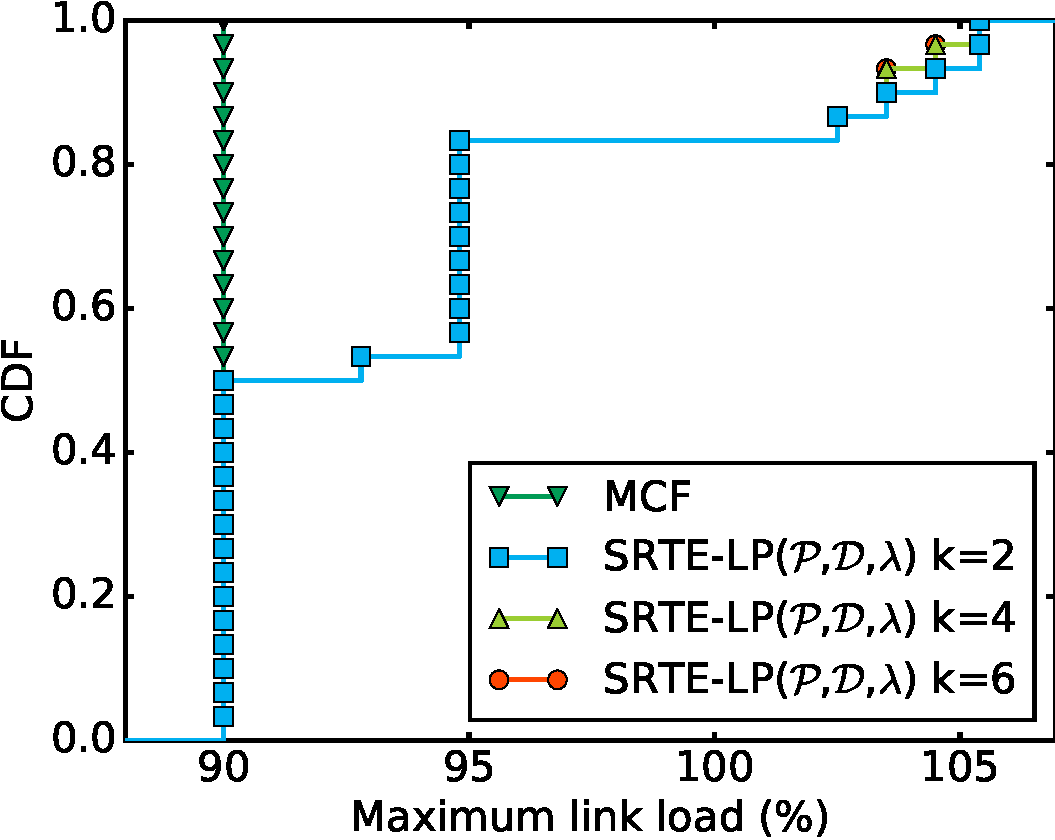
\includegraphics[width=0.8\textwidth]{images/solver_lower_bound_seg_cmp.2016RocketFuelUCL.cdfs.pdf}
\end{center}
\caption{Lower bound}
\label{fig:optimum_lowerbound}
\end{figure}


%The first question to answer is how near \name~really is to the optimality.
\textbf{CG4SR provides solutions whose maximum load is at most 4\% more than the optimal solution.} 
We ran \name~without enabling adjacency segments and without time limit.
The experiment was repeated with limits of 2, 4 and 6 segments
to observe the impact of the segment limit on the quality of the solution.
Figure \ref{fig:optimum:gap} shows CDFs of the gap (in percents)
between the \name~upper and lower bounds
on all the 30 instances (i.e., 5 demand matrices for each of the 6 topologies)
and increasing the limit on the number of segments.
This gap is the maximum distance to the actual optimum.
We can see that increasing the limit from 2 to 4 segments impacts
the quality of the solution while increasing the limit from 4 to 6 has little impact.
Paths with 4 or 6 segments add more flexibility than paths with 2 segments
to SRTE-UTIL-ILP.
We can see that this gap is most of the time below 1\% of the load and at worst 4\% of the load
if 4 segments are allowed.


\begin{figure}
\begin{center}
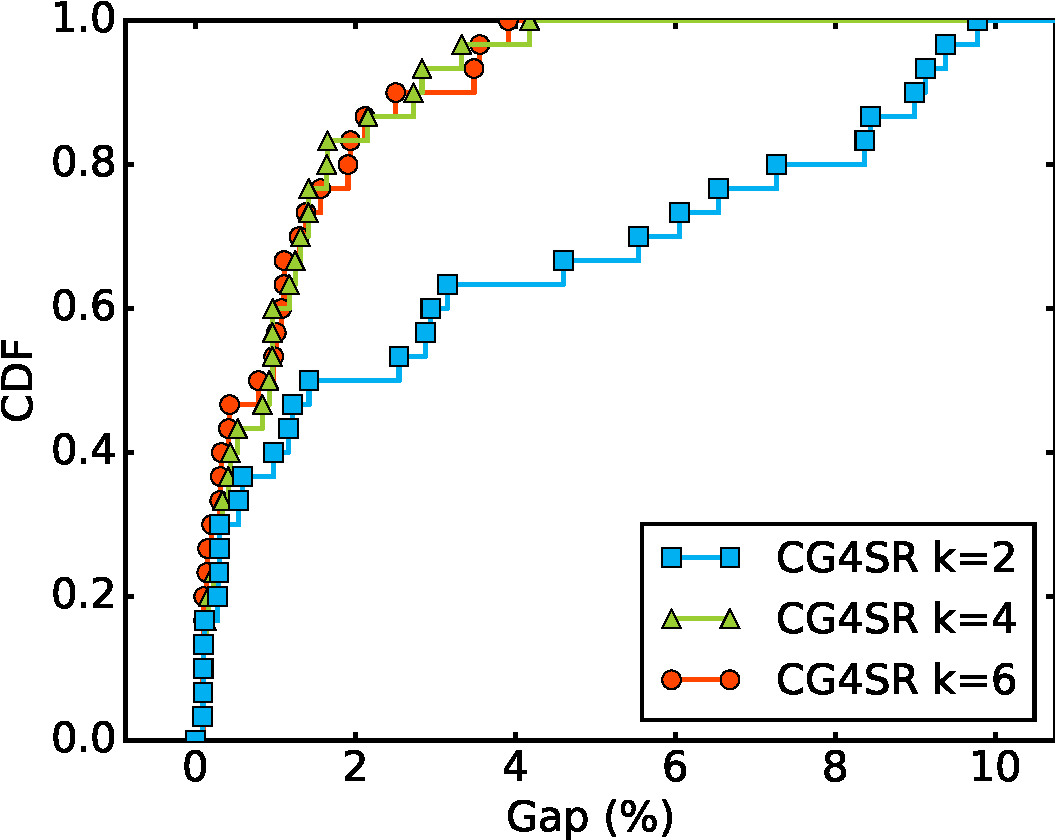
\includegraphics[width=0.8\textwidth]{images/solver_gap_optim_seg_cmp.2016RocketFuelUCL.cdfs.pdf}
\end{center}
\caption{Gap}
\label{fig:optimum:gap}
\end{figure}


\textbf{CG4SR is more efficient than Bhatia and MCF.} 
We compared the speed of \name~to Bhatia, MCF and MCFP. MCFP is an efficient variant of MCF that is only able to
compute the optimal value of MCF, not the actual routing paths.
%All these solvers provide guarantee on their final solutions.
Figure \ref{fig:optimum:time} describes how fast the different solvers can find
their best solution.
During these runs, the limit on the number of generated paths
at each column generation iteration, \textit{maxp} in Algorithm \ref{algo:iterate}, is fixed to 10.
This figure shows a CDF of the execution time on the different topologies and
demand matrices for \name, Bhatia and MCF.
Because Bhatia only allows two segments, \name~is also limited to two segments in this figure.
MCF is the slowest one and it runs out of memory for all the demand matrices
of the largest topology despite the 120GB available.
Bhatia only considers paths that can be expressed with two segments.
This significantly reduces the problem size and Bhatia can always get an answer.
\name~can run with any number of two segments because of the lazy generation of the paths.
And this is so effective than we are actually faster than Bhatia with a two-segment limit.

Figure \ref{fig:optimum:time} also shows that the MCFP variant of MCF
can actually compute the optimal value of the MCF quicker than \name.
But, as mentioned above, MCFP only provides the maximum link
utilisation of the MCF formulation but not a set of paths satisfying it. Hence, in practice, MCFP can
only be used to provide lower bounds which, as we showed in Figure \ref{fig:optimum:gap}, are worse
than the ones provided by our algorithm.

%while the optimal value is the same as the MCF formulation,
%we cannot extract paths that satisfy its optimal value.
%Moreover,there is no guarantee that the MCFP solution is actually reachable,
%nor how far from the real optimal it could be.

\begin{figure}
\begin{center}
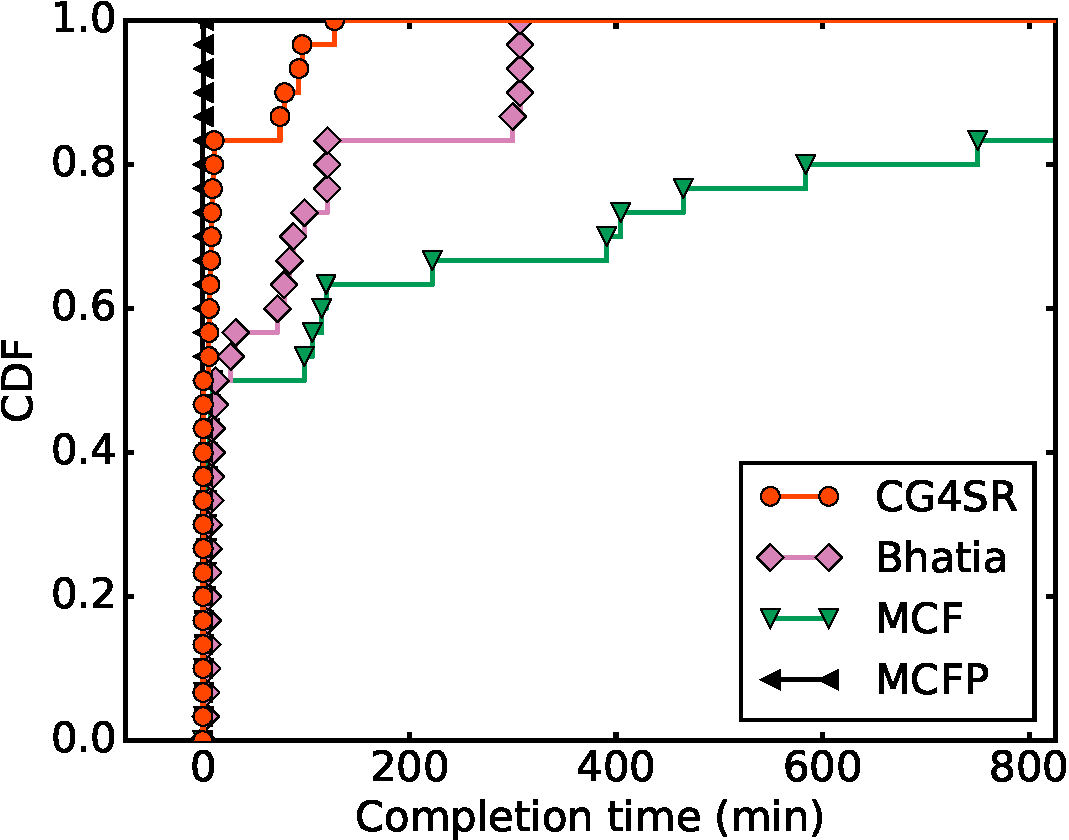
\includegraphics[width=0.8\textwidth]{images/solver_exec_times_inf-2.2016RocketFuelUCL.cdfs.pdf}
\end{center}
\caption{Execution time (\name~is limited to two segments)}
\label{fig:optimum:time}
\end{figure}


\textbf{CG4SR scales better than MCF and Bhatia.}
Our model has fewer variables than the MCF and Bhatia formulations.
The size of our model is the number of paths that were generated.
The size of MCF considers how much of each demand can be placed on each edge.
Therefore, the number of variables is the number of edges multiplied by the number of demands.
Bhatia considers for each demand, two segments through a single node of the graph.
Its number of variables is thus the number of nodes multiplied by the number of demands.
We observe that \name~is more scalable
because it considers at worst 60 times fewer possibilities than Bhatia
and 200 times fewer than MCF. This explains why \name~is faster than Bhatia and MCF.
This difference does not change significantly when varying the limit on the number of segments.
As can be seen in Figure \ref{fig:size:colgen},
the number of generated columns seems to grow linearly with the number of demands.
Given that the restricted path set is initialized with all the direct paths for every demand,
the path-finding process (Algo \ref{algo:iterate}) only creates a limited number
of additional paths to reach optimality.
This also explains why the column generation approach is so efficient in practice, as it only needs to solve the linear program
with a number of variables only slightly above the number of demands.
%\todo{Pierre: Enough dots for conclusions ?}

\begin{figure}
	\centering
	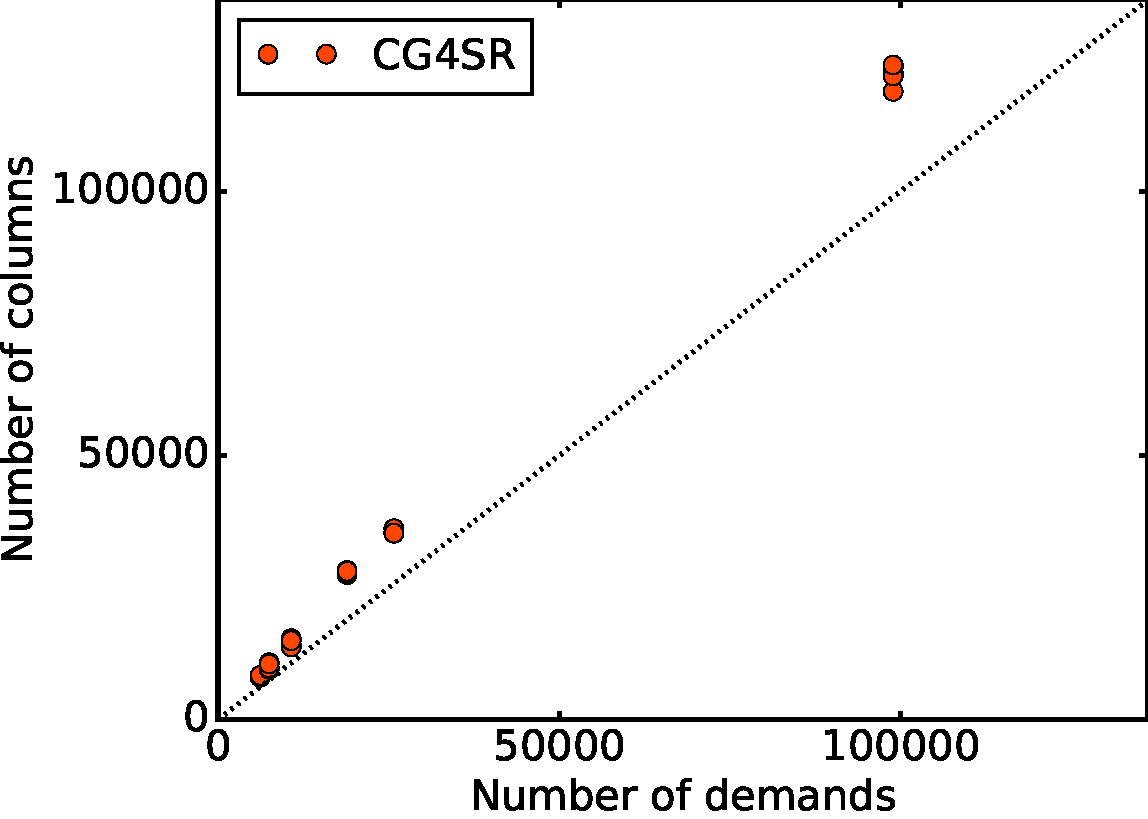
\includegraphics[width=0.8\textwidth]{images/solver_columns_over_demands_inf-6.2016RocketFuelUCL.pdf}
	\caption{Number of generated columns over the size of the demand matrices}
	\label{fig:size:colgen}
\end{figure}


\subsection{Any-time behavior}

The previous section shows that we can produce quality solutions with illimited time budget.
This section evaluates the quality of \name~solutions over time.
We compare \name~ to the heuristic approaches DEFO, SRLS and also to Bhatia.

\textbf{CG4SR finds good solution even if only allowed to run for a short amout of time.}
Figures \ref{fig:anytime:1min}, \ref{fig:anytime:5min}
and \ref{fig:anytime:10min} show, for each of the cited solvers, a CDF of the gap
to the SRTE-LP solution for the cited solvers after,
respectively 1 minute, 5 minutes and 10 minutes.
During these runs, the \textit{maxp} parameter (see Algorithm \ref{algo:iterate}) of \name, is fixed to 10.
The limit of segments is set to 5, except for Bhatia which limits itself to 1.
The quality of a solution is the difference between its current solution and the \name~lower bound
that was computed without time limit and the same limit on the number of segments.

We see that we are always faster than Bhatia even with limited time spans.
SRLS and DEFO are heuristic approaches and therefore are able to quickly find good solutions.
Figure \ref{fig:anytime:1min} shows that \name~ is already comparable to SRLS and better than DEFO
for half of the instances after 1 minute.
We see that DEFO initially finds better solutions but \name~catches up for most of instances
by increasing the timeout in Figure \ref{fig:anytime:5min} and Figure \ref{fig:anytime:10min}.
The largest instance is not yet solved after 10 minutes and that explains why DEFO is still better.

\begin{figure}
\begin{center}
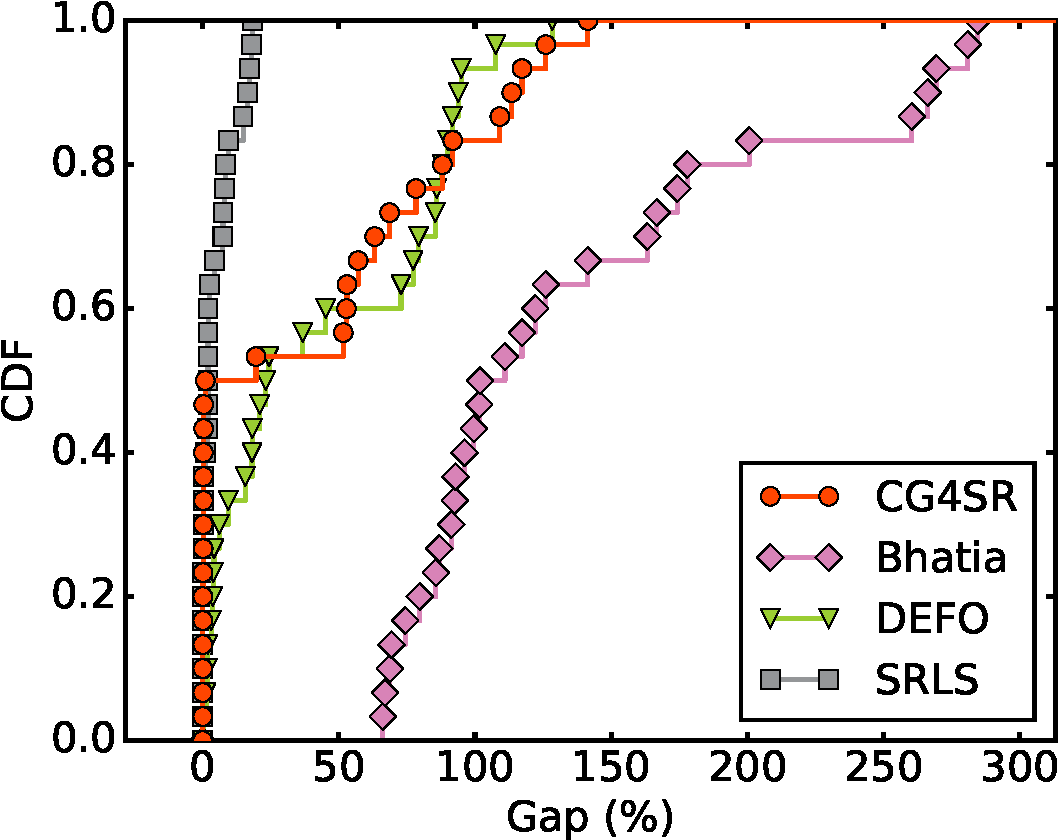
\includegraphics[width=0.8\textwidth]{images/solver_gap_optim_60-6.2016RocketFuelUCL.cdfs.pdf}
\caption{Timeout at 1 minute}
\label{fig:anytime:1min}
\end{center}
\end{figure}

\begin{figure}
\begin{center}
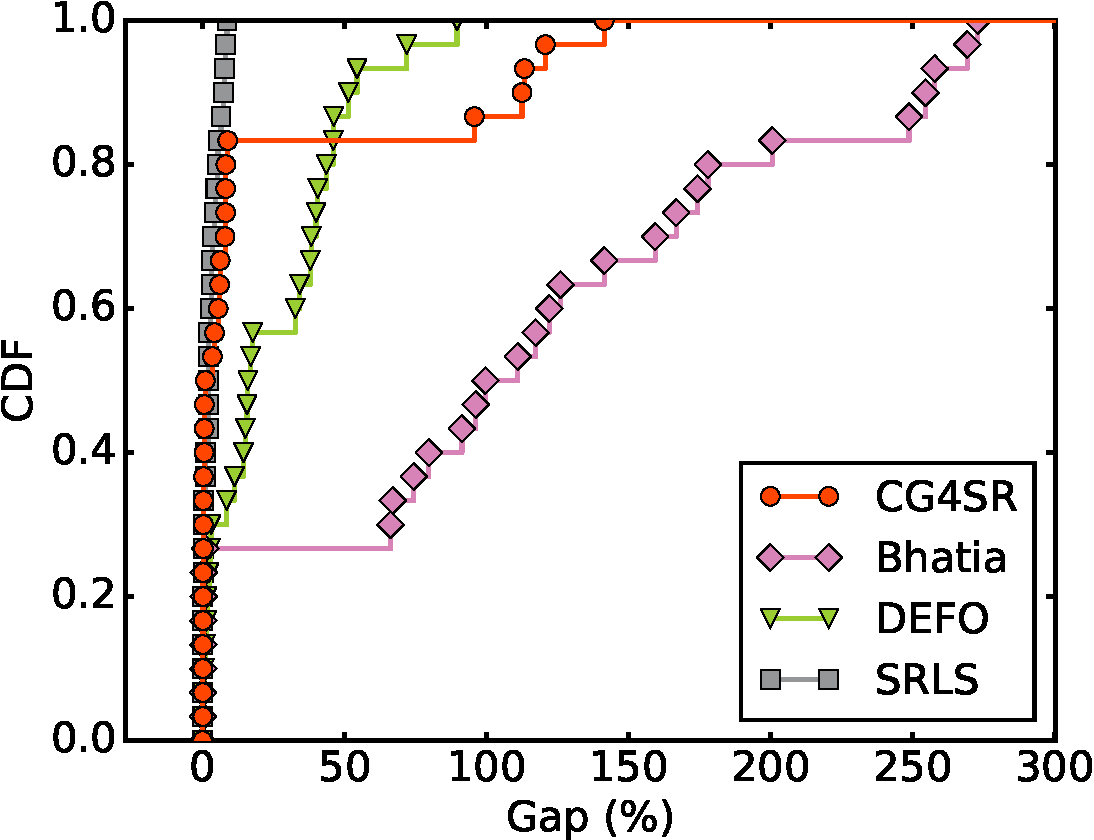
\includegraphics[width=0.8\textwidth]{images/solver_gap_optim_300-6.2016RocketFuelUCL.cdfs.pdf}
\caption{Timeout at 5 minutes}
\label{fig:anytime:5min}
\end{center}
\end{figure}

\begin{figure}
\begin{center}
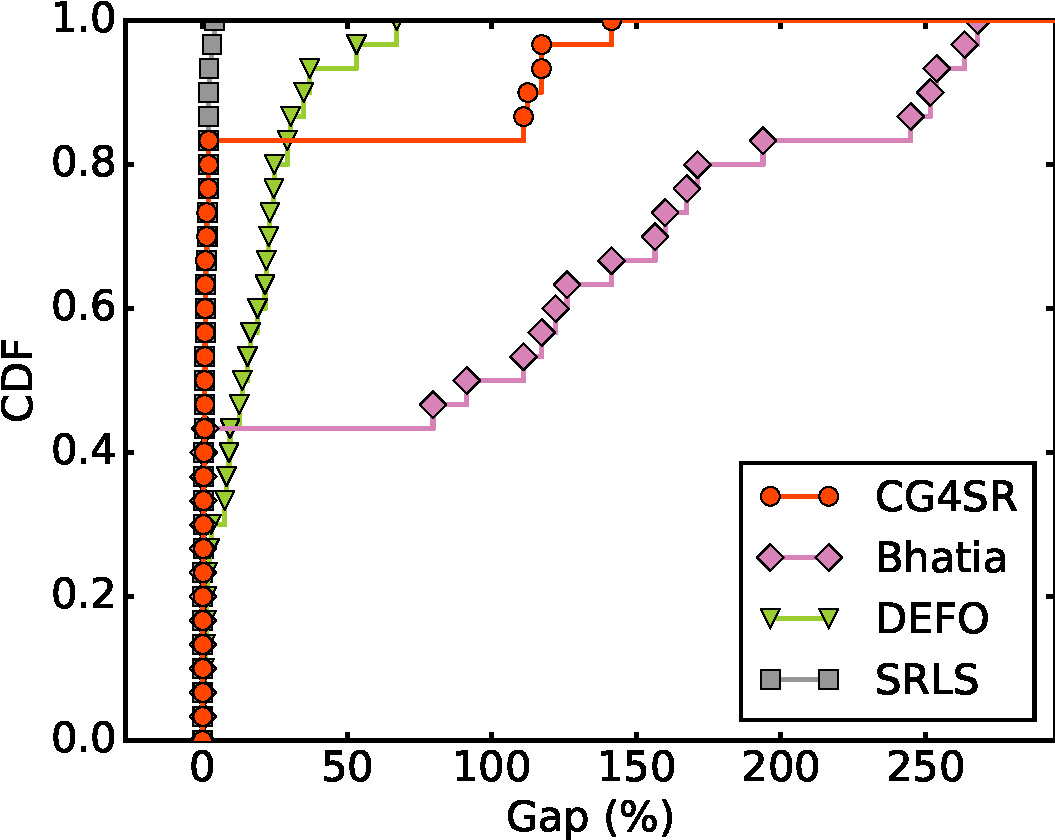
\includegraphics[width=0.8\textwidth]{images/solver_gap_optim_600-6.2016RocketFuelUCL.cdfs.pdf}
\caption{Timeout at 10 minutes}
\label{fig:anytime:10min}
\end{center}
\end{figure}


\textbf{CG4SR is more robust than SRTE over different sets of demands.}
SRLS produces good results but however this solution is based on local search and can be stuck in a local optimum.
We did not observe it on the demand matrices generated by the gravity model.
The demand volumes are generally much lower than link capacities.
This also means that there are many possible ways to reach good solutions,
even if the best solution is hard to find.
The gravity model is a good match to the Traffic Engineering problem in ISPs
but demand volumes are likely higher in inter-datacenter communication \cite{b4}.
This also means that there are fewer good solutions.
We generated one additional demand matrix for each RocketFuel topology
with a low number of large demands requiring 95\% of the bandwidth available
between their source and destination.
Figure \ref{fig:anytime:srlsdefense} shows a CDF of the quality of the solution with
a time limit of 10 minutes and a limit of six segments as in Figure \ref{fig:anytime:10min}.
These results confirm that SRLS can be worse than \name~when fewer good solutions are available.

\begin{figure}
	\centering
	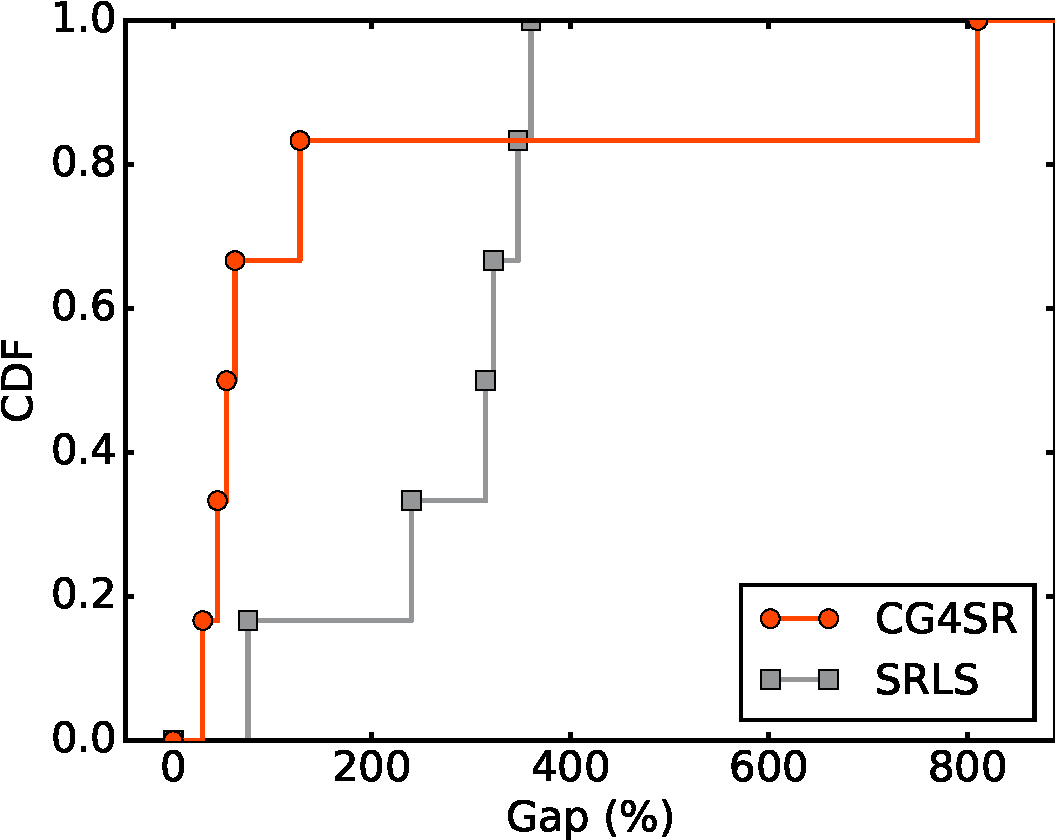
\includegraphics[width=0.8\textwidth]{images/solver_gap_optim_600-6.2016RocketFuelUCL_datacenter.cdfs.pdf}
	\caption{Gaps between $SRTE-LP(\P,\D,\lambda)$ and SRLS or \name~after 10 min with a limit of 6 segments}
	\label{fig:anytime:srlsdefense}
\end{figure}

%\textbf{CG4SR avoids to use SR on too many paths.}
%The gap is not the only criteria of the quality of a solution.
%Since the encoded stack of Segment Routing labels takes space into each packet,
%they take bandwidth resources to be transmitted.
%That is, if two solutions have the same gap to \name~lower bound,
%it's best to choose the one with fewer paths with at least two segments.
%Figure \ref{fig:anytime:10min:detours} shows how many paths need at least two segments to reach the solutions
%in Figure \ref{fig:anytime:10min}.
%We see that Bhatia finds solutions mostly without any segment but they have bad gaps,
%meaning that Bhatia did not have the time to find segments.
%When its gaps are good, it uses 2 segments on almost all the paths.
%\name~cannot find good segments for 5 instances (the demand matrices of the largest topology).
%Yet, for all the other instances, for a similar gap, it detours fewer demands than SRLS.
%DEFO detours fewer paths than \name~ but cannot always reach similar gaps.

%\begin{figure}
%	\centering
%	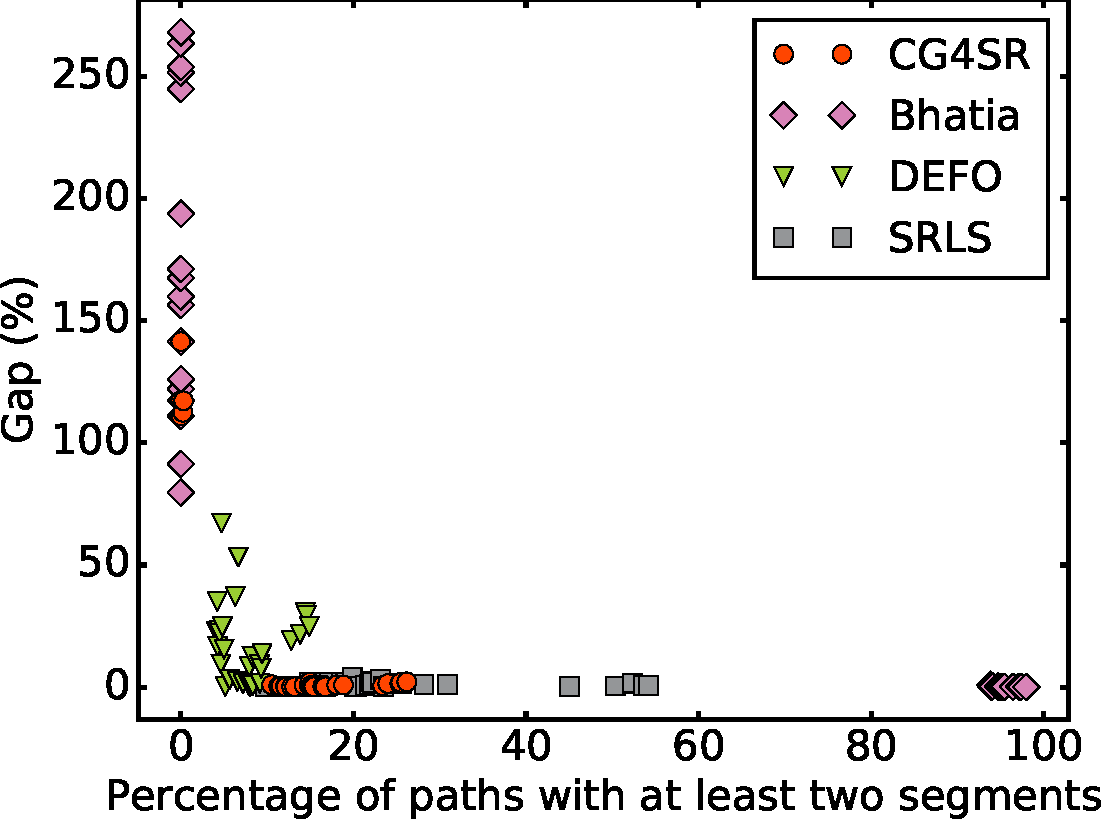
\includegraphics[width=0.3\textwidth]{images/solver_detoured_paths_600-6.2016RocketFuelUCL.pareto.pdf}
%	\caption{Gaps over the percentage of paths with at least two segments. We fixed the time limit to 10 minutes and the limit of segments to 6.}
%	\label{fig:anytime:10min:detours}
%\end{figure}

\subsection{Adjacency segment benefits}

\textbf{Adjacency segments are important in TE and CG4SR is the first to use them.}
\name~is the first SR traffic engineering model to support adjacency segments.
We evaluate the benefits of adjacency segments on the inter-datacenter network topology of OVH
in Europe (described in \cite{scmon}).
This topology has more parallel links than RocketFuel topologies and
thus, the OVH topology can really benefit from adjacency segments.
We do not have access to the link weights and capacities of OVH.
Therefore, for each link bundle we set the capacity of half of the links to some value and the other
half to half of that value. This simulates the link upgrades on the network. For pairs of
nodes with a single link between them, we set the capacity to be ten times bigger.
Five demand matrices were generated for the OVH topology with the gravity model \cite{gravitymodel}.

Figure \ref{fig:adjacency:upperbound} shows CDFs of the gap (in percents)
between the \name~upper and lower bounds over the demand matrices of the OVH topology.
We do not limit the execution time and we limit the number of segments to 4.
This means that we allow at most one detour through a specific link
because one segment is needed for the destination and a link detour costs two segments.
Even allowing only one link detour halves the load of the maximally loaded link
because it utilizes better the parallel links of this topology.

\begin{figure}
	\centering
	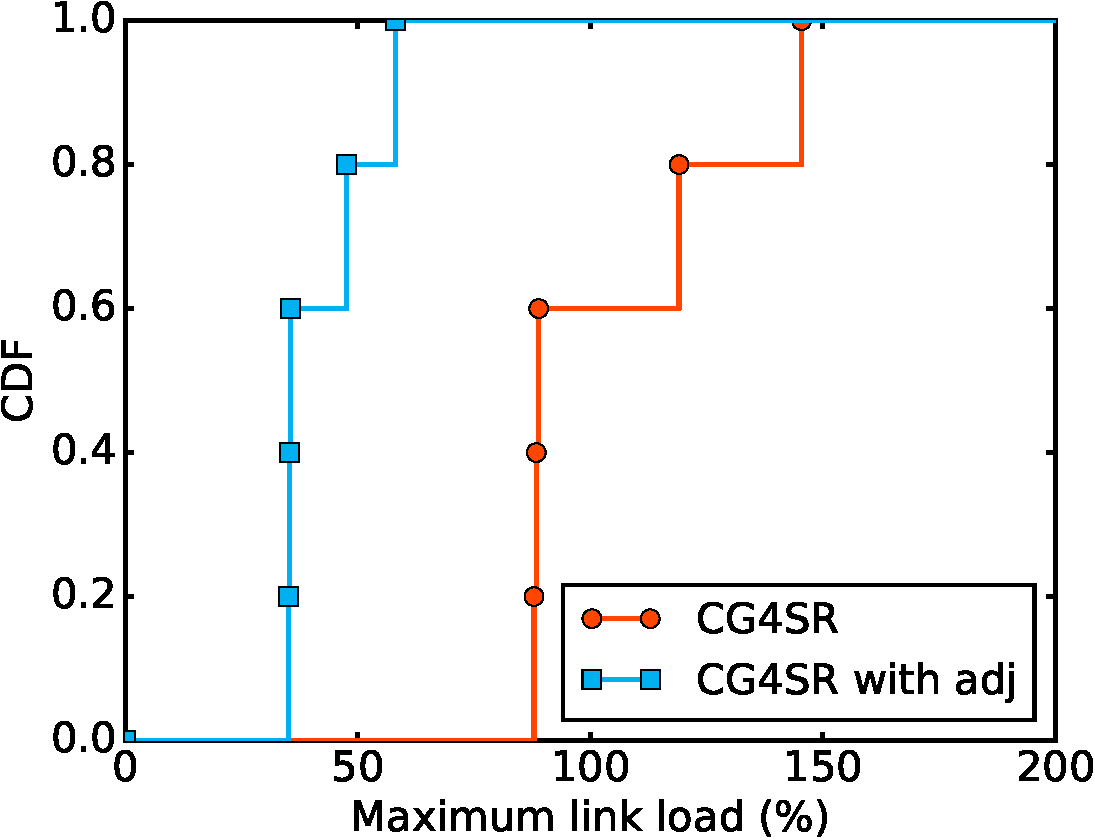
\includegraphics[width=0.8\textwidth]{images/solver_adj_upper_bound.OVH_paper.cdfs.pdf}
	\caption{The \name~solutions with or without adjacency segments. The limit of segments is fixed to 4.}
	\label{fig:adjacency:upperbound}
\end{figure}



\section*{Conclusion}

In this chapter we propose                                                                                                                                                                                                                                                                                                                                                                                                                   the first solution to exploit column generation to solve segment routing problems.
We believe that column generation is a good approach for solving segment routing problem and reinforce this
belief in the next chapter. The structure of sr-paths make it amiable to dynamic programming algorithms so
we feel that it will often be the case that the pricing problem will have a nice DP optimal substructure.

Our solution improves the state of the art lower bound making it possible to better evaluate the quality
of heuristic solutions. We also showed that even tough we are slower on demands generated according to a 
gravity model, with more constrained demands we can actually be much more efficient than local search.

It still remains an open problem to find an algorithm capable of providing optimal solution to the TE problem 
over segment routing within reasonable amount of time. We are unsure whether wrapping our solution with a branch-and-price
is the right way to go but it is certainly an interesting possibility.

\chapter{Network monitoring with segment routing}
\label{chapter:scmon}


\section*{Introduction}

Monitoring is a crucial task for network operations. It is needed to ensure that all resources operate correctly (e.g., no
failures) and their configuration meets operator’s expectations (no congestion, required quality of service, etc.). Effective
monitoring is also fundamental for management tasks like traffic engineering, maintenance and troubleshooting.

\begin{figure}
\begin{center}
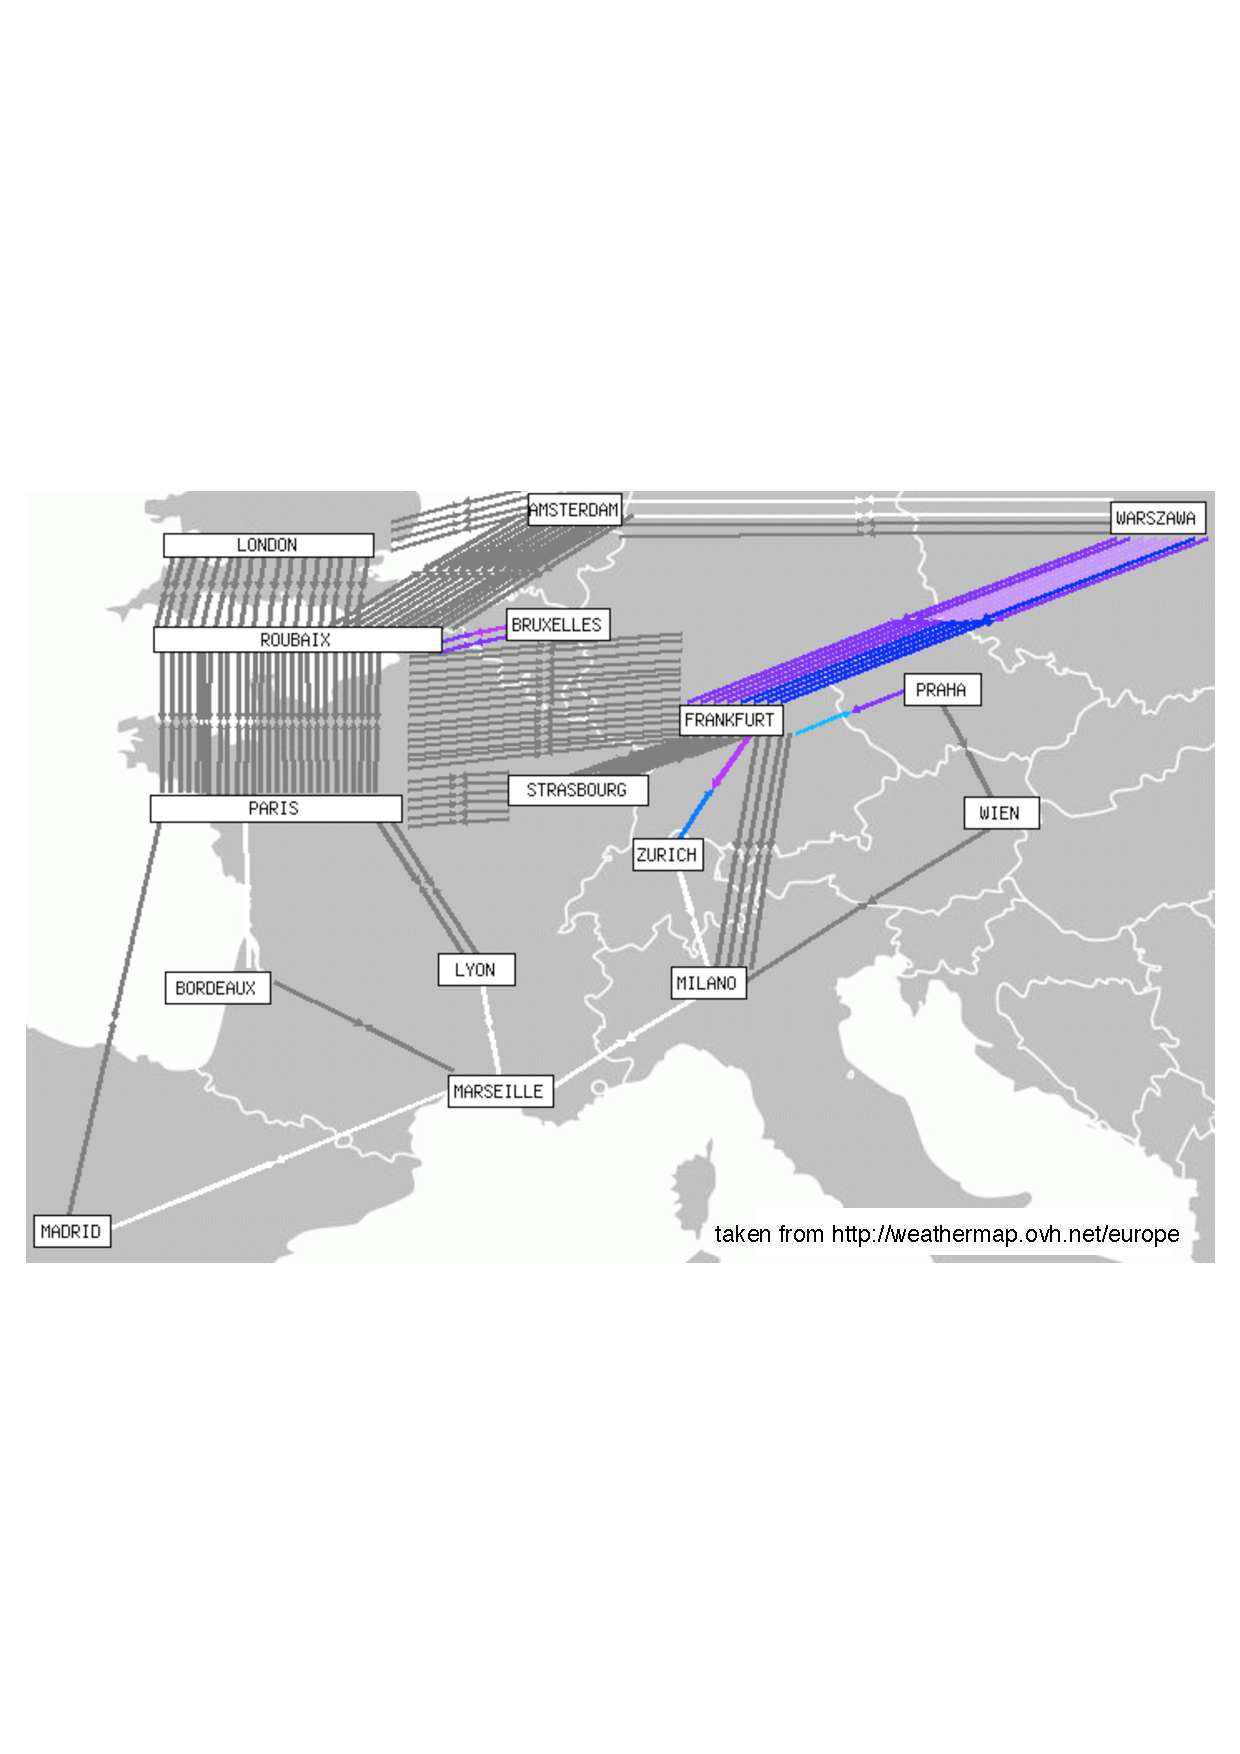
\includegraphics[width=.85\columnwidth]{figures/ovh-eu.pdf}
\end{center}
\caption{European backbone of \textsf{OVH}. In contrast to prior techniques, our algorithm can monitor health and performance of single
links in bundles (e.g., between \textsf{LONDON} and \textsf{ROUBAIX}).}
\label{fig:ovh}
\end{figure}


Unfortunately, even basic monitoring tasks, like checking for hardware malfunctions, are practically hard, due to the
complexity of current networks. Prominently, multi-path routing is widely used, both to spread the load on multiple paths
and to aggregate parallel links in bundles.
Figure \ref{fig:ovh} shows an overview of the European backbone of a big cloud provider,
\textsf{OVH}. It highlights that parallel links are used at the same time between many pairs of routers. While enabling better
performance and robustness, multi-path routing also poses significant obstacles to monitoring. For instance, assessing
the exact path and performance of each packet becomes complex [2], [20] since such a path depends on (vendor-specific) hash functions used by routers for load-balancing.

As a consequence, not only naive approaches (e.g., based on ping or traceroute) are not sufficient, but also 
state-of-the-art monitoring techniques tend to be ineffective.


On the one hand, protocol-based approaches use control-plane messages to infer possible failures. 
For example, link-state routing protocols (like OSPF or IS-IS) or specialized
ones (BFD [14]) rely on heartbeat-like mechanisms to check
bi-directional connectivity among pairs of adjacent nodes. This
approach only ensures detection of failures that affect control plane messages. 
However, it cannot be used to detect failures that only affect data-plane traffic like: 

\begin{enumerate}[i)]
\item corruption of an
optical link that leads to framing errors and packet losses;
\item malfunctioning of a router interface that considers the link still up but discards all the received packets;
\item failure of only one link among the parallel ones between two routers.
\end{enumerate}

On the other hand, probe-based techniques rely on sending
data-plane monitoring packets, i.e., probes, between fixed
vantage points in the network. Vantage points typically run
standard protocols (e.g., IPSLA [8]) to send probes and extract
measurements from them. Unfortunately, if the probes are sent
over paths used to forward regular traffic, many vantage points
may be needed to obtain high coverage, and links not used
by current paths (e.g., backup links) cannot be checked at
all. Otherwise, probes can be sent over tunnels (e.g., RSVP-TE [3] ones) to enforce specific paths, but this is not scalable.
Indeed, even for detecting single-link failures and pinpointing
their position, the number of needed tunnels tends to explode,
and so does the control-plane overhead (to signal tunnels) [7].

We propose a new technique that ensures full coverage of all network resources from a
single vantage point. It is based on sending data-plane probes over carefully-chosen cycles. This way, a single box can both
send and receive monitoring probes, avoiding the need for synchronizing and coordinating multiple vantage points, hence
minimizing infrastructural costs. By relying on data-plane measurements, we support both detection of hardware failures and resource overloading (e.g., link congestion).

% Segment routing generates conflicting objectives for the computation
% of cycles over which probes are sent. On the one hand, we would like to minimize the number of cycles, to reduce the
% monitoring overhead; hence, we should have cycles that are long and few in number. On the other hand, we need cycles
% to be enforced in practice, and long cycles may require too many segments even for the most powerful commercial routers
% (currently supporting less than 10 segments). To tackle those challenges, SCMon runs original algorithms
% that compute cycles on a monitoring topology, maintained by routers in addition to the one used for user traffic. The monitoring topology spans all network links, 
% and uses carefully computed weights that avoid (as much as possible) ECMP paths, i.e., multiple shortest paths between a pair of nodes.
% Note that existing routers have already been shown to well support two topologies and their (limited) overhead [17].
% SCMon supports detection and localization of any set of link failures/overloading. It infers single-link failures by keeping
% track of the cycles associated to probes sent and not received at the monitoring box. For multiple link failures, we have two
% cases. Some of them, e.g., affecting links in disjoint cycles, are detected directly from the set of lost probes (as single-link failures). 
% The others, e.g., affecting two links belonging to a single monitoring cycle, are reported by SCMon one at
% a time: This provides operators with a debugging interface (asking to correct one error before showing another one)
% similar to the one of a compiler for software programs. Similar considerations apply to node failures and link congestion.
% In developing SCMon, we make three main contributions.
% 
% Our approach to compute monitoring cycles consists of four steps.
% The first step computes IGP weights for the monitoring topology, in order to minimize ECMP paths.
% The second step models link bundles aggregated into a single IGP link. 
% The third step calculates a set of cycles covering the whole network and sharing the node from which probes are sent.
% The last step computes the SR segments to send probes over those cycles.


%In this section we will propose several algorithms and strategies to compute a cycle cover of the network
%using segment routing. We need however to impose some properties in the cycle cover in order to be able to use
%it for detecting single link failures in a network. Those properties as the following:

As usual, we start by defining the problems that we tackle in this chapter. To do that we need the two following definitions.
Throughout this chapter we assume that the network topology is symmetric.

\begin{definition}
Let $G$ be a symmetric network, $s \in V(G)$ and $k \in \mathbb{N}$. We denote by $\mathcal{C}^k_s$ the set of deterministic sr-cycles from $s$ to $s$ with segment cost at most $k$.
\end{definition}

\begin{definition}
Let $G$ be a symmetric network, $s \in V(G)$ and $k \in \mathbb{N}$. A \emph{$k$ sr-cycle cover} of a network $G$ 
with vantage point $s$ is a subset $C \subseteq \mathcal{C}^k_s$ of deterministic sr-cycles such
that for each edge $e \in E(G)$ there exists $\sr{c} \in C$ such that $e \in E(\sr{c})$.
\end{definition}

Below we define the two problems that we tackle in this chapter. Both of them seek to compute a cycle cover.
The first aims at minimizing the maximum segment cost of any sr-cycle in the cover while the second wants to minimize the number of cycles for a given segment cost limit.
% We will see that the first problem admits a polynomial time solution and that the second one is \NPhard.


\begin{problem}{Min segment cost cover}
\label{prob:min-seg-cover}
\textbf{Input:} A symmetric network $G$ and $s \in V(G)$.

\textbf{Output:} A sr-cycle cover $C$ of $G$ such that the maximum segment cost of any sr-cycle $\sr{c} \in C$ is minimum.
\end{problem}

\begin{problem}{Min sr-cycle cover}
\label{prob:min-cycle-cover}
\textbf{Input:} A symmetric network $G$, $s \in V(G)$ and $k \in \mathbb{N}$.

\textbf{Output:} A sr-cycle cover $C \subseteq \Csk$ of $G$ such that $|C|$ is minimum.
\end{problem}
% 
% \begin{proposition}
% Problem \ref{prob:min-cycle-cover} is \NPhard.
% \end{proposition}
% 
% \begin{proof}
% The problem of finding a minimum cardinaly cycle cover of a graph is \NPhard and by setting $k$
% large enough and setting IGP weights such that there is not ECMP any solution
% to Problem \ref{prob:min-cycle-cover} corresponds to a minimum cycle cover.
% \end{proof}
% 


\section{Minimum segment cost covers}

In this section we propose a polynomial time algorithm for solving Problem \ref{prob:min-seg-cover}.
We have seen in Chapter \ref{chapter:sr} reachability results that tells us exactly how costly,
in terms of segments, it is to deterministically reach a given node in the network. Using these results
we can easily establish how costly it is to cover a given edge with a deterministic sr-cycle.

In order to cover a given edge $e$ with a deterministic sr-cycle from $s$ to $s$ with segment cost at most
$k$, we have essentially two options:

\begin{enumerate}
 \item First we go from $s$ to some node $x$ using a deterministic sr-path of cost, say, $k_1$. Then travel
 from $x$ to some node $y$ via a unique shortest path that contains edge $e$. Finally, we go from $y$ back to $s$
 with a deterministic sr-path of cost $k_2 = k - k_1$. This is illustrated in Figure \ref{fig:cover-edge1}.
 
\begin{figure}
\begin{center}
\begin{tikzpicture}
\def\x{0}
\def\y{0}

\node[scale=0.15] (s) at (0 + \x, 0 + \y)  {\router{s}{router}};
\node[scale=0.15] (x) at (-2 + \x, 2 + \y) {\router{x}{router}};
\node[scale=0.15] (y) at (2 + \x,  2 + \y) {\router{y}{router}};

\draw[line width=2, black] (s) edge[below, sloped, bend left, dashed, ->] node[black] {
\footnotesize
\begin{tabular}{c}
 sr-path from $s$ to $x$ \\
 of cost at most $k_1$
\end{tabular}
} (x);
\draw[line width=2, black] (y) edge[below, sloped, bend left, dashed, ->] node[black] {
\footnotesize
\begin{tabular}{c}
 sr-path from $y$ to $s$ of \\
 cost at most $k - k_1$
\end{tabular}
} (s);

\draw[line width=2, black] (x) edge[above, sloped, dashed, ->] node[black,font=\bfseries] {\texttt{$SP(x, y)$}} (y);

\draw[line width=3] (-0.5, 2) edge[below, ->] node {$e$} (0.5, 2);

\end{tikzpicture}
\end{center}
\caption{First case of edge covering.}
\label{fig:cover-edge1}
\end{figure}

 
 \item The second way to cover $e$ is to use an adjacency segment over it. To do so, we first go from $s$ to
 some node $x$ with a deterministic sr-path of cost at most, say, $k_1$. This node $x$ must be such that it contains 
 a unique shortest path to $e^1$. Otherwise the resulting cycle would not be deterministic. Then we use an adjacency 
 segment on $e$ to traverse it by following the unique shortest path between $x$ and $e^1$ and then $e$.
 Then we go to some node $y$ via a unique shortest path from $e^2$. Finally, we go from $y$ back to $s$ with a
 sr-path of cost at most $k_2 = k - k_1 - 2$. The $-2$ comes from the fact that we spent a segment cost of $2$ 
 with the adjacency segment $e$. This case is illustrated in Figure \ref{fig:cover-edge2}.

\begin{figure}
\begin{center}
\begin{tikzpicture}
\def\x{0}
\def\y{0}

\node[scale=0.15] (s) at (0 + \x, 0 + \y)  {\router{s}{router}};
\node[scale=0.15] (x) at (-3.5 + \x, 2 + \y) {\router{x}{router}};
\node[scale=0.15] (y) at (3.5 + \x,  2 + \y) {\router{y}{router}};
\node[scale=0.15] (u1) at (-1 + \x,  2 + \y) {\router{$u_1$}{router}};
\node[scale=0.15] (u2) at (1 + \x,  2 + \y) {\router{$u_2$}{router}};

\draw[line width=2, black] (s) edge[below, sloped, bend left, dashed, ->] node[black] {
\footnotesize
\begin{tabular}{c}
 sr-path from $s$ to $x$ \\
 of cost at most $k_1$
\end{tabular}
} (x);
\draw[line width=2, black] (y) edge[below, sloped, bend left, dashed, ->] node[black] {
\footnotesize
\begin{tabular}{c}
 sr-path from $y$ to $s$ of \\
 cost at most $k - k_1 - 2$
\end{tabular}
} (s);

\draw[line width=2, black] (x) edge[above, sloped, dashed, ->] node[black,font=\bfseries] {\texttt{$SP(x, u_1)$}} (u1);
\draw[line width=2, black] (u2) edge[above, sloped, dashed, ->] node[black,font=\bfseries] {\texttt{$SP(u_2, y)$}} (y);


\draw[line width=3] (u1) edge[below, ->] node {$e$} (u2);

\end{tikzpicture}
\end{center}
\caption{Second case of edge covering.}
\label{fig:cover-edge2}
\end{figure} 
\end{enumerate}

Note that in both cases, nothings prevents us to have $x = e^1$ or $y = e^2$. We do not require these nodes to be distinct
as doing so would provide an incomplete description of all possible cases.

Next we prove formally that those two cases cover all possibilities. The next theorem directly translate into
a polynomial time algorithm for computing minimum segment cost covers.

\begin{theorem}
\label{thm:edge-cover}
Let $G$ be a network $s \in V(G)$, $e \in E(G)$ and $k \in \mathbb{N}$ an integer. There exists a deterministic sr-cycle $\sr{c}$
from $s$ to $s$ of cost at most $k$ such that $e \in E(\sr{c})$ if and only if there exist integers $k_1, k_2 \geq 1$, $x \in \nreach(k_1, s)$, $y$ such that $s \in \nreach(k_2, y)$ 
and one of the two following conditions holds
\begin{enumerate}[(1)]
 \item $k_1 + k_2 = k$, $y \in \spreach(x)$ and $e \in \sp(x, y)$
 \item $k_1 + k_2 = k - 2$, $e^1 \in \spreach(x)$ and $y \in \spreach(e^2)$
\end{enumerate}
\end{theorem}

\begin{proof}
Let $G$ be a network $s \in V(G)$, $e \in E(G)$ and $k \geq 1$ an integer.

$(\Rightarrow)$ Assume that there exists a deterministic sr-cycle $\sr{c}$ from $s$ to $s$
with $\cost(\sr{c}) \leq k$ such that $e \in E(\sr{c})$. Write $\sr{c} = \langle x_1, \ldots, x_l \rangle$.
Since $e \in E(\sr{c})$ there exists $i \in \{1, \ldots, l\}$ such that either $x_i = e$ or $i < l$ and
$e \in \sp(x^2_{i}, x^1_{i + 1})$.

\emph{Case 1:} $e \in \sp(x^2_{i}, x^1_{i + 1})$. Let $x = x^2_{i}$ and $y = x^1_{i + 1}$. Then $\sr{p} = \langle x_1, \ldots, x_{i} \rangle$ is a deterministic sr-path
from $s$ to $x$ of cost, say, $k_1$ and $\sr{q} = \langle x_{i + 1}, \ldots, x_l \rangle$ is a deterministic sr-path from $y$ to $s$ of cost $k_2 \leq k - k_1$. 
Therefore, $x \in \nreach(k_1, s)$, $s \in \nreach(k_2, y)$. Since $\sr{c}$ is deterministic, there is a unique shortest path
from $x$ to $y$ so $y \in \spreach(x)$. Since by hypothesis $e \in \sp(x, y)$, condition $(1)$ holds.

\emph{Case 2:} $e = x_i$. Let $x = x^2_{i - 1}$ and $y = x^1_{i + 1}$. Then $\sr{p} = \langle x_1, \ldots, x_{i - 1} \rangle$ is a deterministic sr-path
from $s$ to $x$ of cost, say $k_1$, and $\sr{q} = \langle x_{i + 1}, \ldots, x_l \rangle$ from $y$ to $s$ of cost, say $k_2$, such that
$k_1 + k_2 = \cost(\sr{p}) + \cost(\sr{q}) = \cost(\sr{c}) - 2 \leq k - 2$. Thus $x \in \nreach(k_1, s)$ and $s \in \nreach(k_2, y)$.
Since $\sr{c}$ is deterministic, there is a unique shortest path from $x = x^2_{i - 1}$ and $e^1 = x^1_i$. For the same reason,
there exists a unique shortest path from $e^2 = x^2_i$ to $y = x^1_{i + 1}$.  Thus $e^1 \in \nreach(2, x)$ and $y \in \spreach(e^2)$ so that
condition $(2)$ holds.

Note that in the first case we have $k_1 + k_2 \leq k$ and in the second $k_1 + k_2 \leq k - 2$ instead of the equalities. 
This is not a problem because if we have a solution with $k_1' + k_2' < k$ we also have a solution with longer paths. The same is
true for $k_1' + k_2' < k - 2$. One way to do so is to add the source $s$ enough times so that both paths have the desired segment cost.

$(\Leftarrow)$ Assume that there exist integers $k_1, k_2 \geq 1$, $x \in \nreach(k_1, s)$, $y$ such that $s \in \nreach(k_2, y)$ 
and either $(1)$ or $(2)$ holds. Since $x \in \nreach(k_1, s)$ there exists a deterministic sr-path
$\sr{p} = \langle x_1, \ldots, x_l \rangle$ from $s$ to $x$ with $\cost(\sr{p}) \leq k_1$. In the same way, since $s \in \nreach(k_2, y)$,
there exists a deterministic sr-path $\sr{q} = \langle y_1, \ldots, y_r \rangle$ from $y$ to $s$ with $\cost(\sr{q}) \leq k_2$.

\emph{Case 1:} Condition $(1)$ holds so that $k_1 + k_2 = k$, $y \in \spreach(x)$ and $e \in \sp(x, y)$. 
Let $\sr{c} = \sr{p} + \sr{q} = \langle x_1, \ldots, x_l, y_1, \ldots, y_r \rangle$. 
This sr-path is deterministic because $y^1_1 = y \in \spreach(x) = \spreach(x^2_l)$. 
For the other indexes, the unicity of shortest paths comes from the fact that both $\sr{p}$ and $\sr{q}$
are deterministic. Since $\sr{c}$ goes from $s$ to $s$ and has cost $k_1 + k_2 = k$, $\sr{c}$ is a sr-cycle of cost at most $k$ from $s$ to $s$.
It contains $e$ because $e \in \sp(x, y) = \sp(x^2_l, y^1_1)$.

\emph{Case 2:} Condition $(2)$ holds so $k_1 + k_2 = k - 2$, $e^1 \in \spreach(x)$ and $y \in \spreach(e^2)$. Let $\sr{c} = \langle x_1, \ldots, x_l, e, y_1, \ldots, y_r \rangle$.
Since $e^1 \in \spreach(x)$ and $y \in \spreach(e^2)$ we have that $\sr{c}$ is deterministic. As before, for the other indexes determinism comes from the 
determinism of $\sr{p}$ and $\sr{q}$. Finally, $\cost(\sr{c}) = \cost(\sr{p}) + \cost(\sr{q}) + \cost(e) = k_1 + k_2 + 2 \leq k - 2 + 2 = k$. Clearly $e \in \sr{c}$
so the proof is complete.
\end{proof}

Theorem \ref{thm:edge-cover} gives necessary and sufficient conditions for the existence of a sr-cycle with segment cost at most $k$
covering a given network edge. This condition is checkable in polynomial time since, if nothing better, we can just loop over all possible
candidates $x, y \in V(G)$ and splits of $k$ into $k_1, k_2$ (recall that $k \leq 2|E(G)|$).

This shows that we can solve Problem \ref{prob:min-seg-cover} in polynomial time. For each edge $e$ we compute the smallest $k$ such that
there exists a deterministic sr-cycle covering $e$. Then the maximum value over all these $k$ values will be the minimum segment cost
for which a sr-cycle cover is possible.

Algorithm \ref{algo:build-cycle} closely follows Theorem \ref{thm:edge-cover} to build a sr-cycle for a given edge $e$, source $s$ and segment cost $k$.
On lines \ref{line:case1-cycle} to \ref{line:case1-cycle-end} we try to see whether there exists $x, y, k_1$ and $k_2$ that satisfy condition $(1)$ from the 
theorem. If so, we build a cycle accordingly by putting together a deterministic sr-path from $s$ to $x$ of segment cost at most $k_1$ and a deterministic sr-path
from $y$ to $s$ of segment cost at most $k_2$. Upon failing to find such a cycle, on lines \ref{line:case2-cycle} through \ref{line:case2-cycle-end} we try to find 
$x, y, k_1$ and $k_2$ that satisfy condition $(2)$ from the theorem. If we find such values, we build a cycle composed by a deterministic sr-path from $s$ to $x$ of cost at most $k_1$,
followed by an adjacency segment on $e$ and a deterministic sr-path from $y$ to $s$ of cost at most $k_2$. If we reach line $16$ then Theorem \ref{thm:edge-cover} guarantees that
there exists no sr-cycle of segment cost at most $k$ that covers $e$ from source $s$.

\begin{algorithm}[t]
\small
\caption{$\textsf{build-srcycle}\left( G, s, k, e \right)$}
\begin{algorithmic}[1]
%\algrule
\cmtline{look for a cycle that satisfies the first set of conditions from Theorem \ref{thm:edge-cover}}
\FOR{$k_1 \in \{ 1, \ldots, k - 1\}$} \label{line:case1-cycle}
  \STATE $k_2 \gets k - k_1$
  \FOR{$x \in \nreach(k_1, s)$}
    \FOR{$y \in \spreach(x)$}
      \IF{$s \in \nreach(k_2, y)$ \textbf{and} $e \in E(\sp(x, y))$}
	\RETURN $\textsf{build-det-srpath}(G, k_1, s, x) \oplus \textsf{build-det-srpath}(G, k_2, y, s)$
      \ENDIF
    \ENDFOR
  \ENDFOR
\ENDFOR \label{line:case1-cycle-end}
\cmtline{look for a cycle that satisfies the second set of conditions from Theorem \ref{thm:edge-cover}}
\FOR{$k_1 \in \{ 1, \ldots, k - 2\}$}  \label{line:case2-cycle}
  \STATE $k_2 \gets k - k_1 - 2$
  \FOR{$x \in \nreach(k_1, s)$}
    \IF{$e^1 \in \spreach(x)$}
      \FOR{$y \in \spreach(e^2)$}
	\IF{$s \in \nreach(k_2, y)$}
	  \RETURN $\textsf{build-det-srpath}(G, k_1, s, x) \oplus \langle e \rangle \oplus \textsf{build-det-srpath}(G, k_2, y, s)$
	\ENDIF
      \ENDFOR
    \ENDIF
  \ENDFOR
\ENDFOR  \label{line:case2-cycle-end}
\RETURN \textbf{null}
\end{algorithmic}
\label{algo:build-cycle}
\end{algorithm}

By pre-computing $\nreach$ and $\spreach$ as sets with $O(1)$ membership testing, this algorithm runs in $O(k^2 \cdot |V(G)|^2 \cdot |G|)$ since the cost 
of building a path with Algorithm \ref{algo:build-det-srpath} is $O(k \cdot |G|)$. In practice thought, it will usually run much faster since the reachability sets are often quite smaller than $V(G)$ and a lot of loop iterations are cut-off beforehand by the conditions.

To check whether a cycle cover exists for a given source $s$ and segment cost $k$ we simply loop over all edges $e \in E(G)$ and check whether a cycle exists
for each of them using Algorithm \ref{algo:build-cycle}. Therefore the runtime of this algorithm is $O(k^2 \cdot |V(G)|^2 \cdot |G| \cdot |E(G)|)$. For 
completeness a formalization of this algorithm is provided as Algorithm \ref{algo:cover-exists}.

\begin{algorithm}[t]
\small
\caption{$\textsf{cover-exists}\left( G, s, k \right)$}
\begin{algorithmic}[1]
%\algrule
\FOR{$e \in E(G)$}
  \IF{$\textsf{cycle-exists}(G, s, k, e) = \textbf{null}$}
    \RETURN \textbf{false}
  \ENDIF
\ENDFOR
\RETURN \textbf{true}
\end{algorithmic}
\label{algo:cover-exists}
\end{algorithm}

To find $k$ such that a cover exists from source $s$, we perform a binary search of $k$ to find the smallest $k$ such that a cover exists. This process is described
in Algorithm \ref{algo:min-seg-cover}. Our initial search interval is $[0, 2|E(G)|]$ because we know from Lemma \ref{lemma:seg_exists}
 that any path admits a segmentation of cost at most $2 |E(G)|$.
Once we find this minimum $k$, we compute a set of sr-cycles that cover all edges. For this we iterate over all edges and compute a sr-cycle covering it with Algorithm \ref{algo:build-cycle}.
We keep a set of covered edges to which we add all edges of every new sr-cycle in the cover. In this way we reduce the total number of cycles in the final solution.
This give a total runtime of $O(\log E(G) \cdot k^2 \cdot |V(G)|^2 \cdot |G| \cdot |E(G)|)$. If the source is unknown, we can add an extra iteration over all $v \in V(G)$ to find the one 
minimizing $k$ as shown in Algorithm \ref{algo:min-seg-cover2}.


\begin{algorithm}[t]
\small
\caption{$\textsf{min-seg-cover}\left( G, s \right)$}
\begin{algorithmic}[1]
%\algrule
\cmtline{perfom a binary search to find the smallest $k$ such that a cover exists}
\STATE $lb \gets 0$
\STATE $up \gets 2|E(G)|$
\WHILE{$up - lb \geq 2$}
  \STATE $k \gets \frac{lb + up}{2}$
  \IF{$\textsf{cover-exists}\left( G, s, k \right)$}
    \STATE $up \gets k$
  \ELSE
    \STATE $lb \gets k$
  \ENDIF
\ENDWHILE
\cmtline{$k = up$ is the smallest segment cost such that a cover exists, build it}
\STATE $covered \gets \emptyset$
\STATE $C \gets \emptyset$
\FOR{$e \in E(G)$}
  \IF{$e \notin covered$}
    \STATE $\sr{c} \gets \textsf{build-srcycle}\left( G, s, ub, e \right)$
    \STATE $covered \gets covered \cup E(\sr{c})$
    \STATE $C \gets C \cup \{ \sr{c} \}$
  \ENDIF
\ENDFOR
\RETURN $C$, $ub$
\end{algorithmic}
\label{algo:min-seg-cover}
\end{algorithm}


\begin{algorithm}[t]
\small
\caption{$\textsf{min-seg-cover}\left( G \right)$}
\begin{algorithmic}[1]
%\algrule
\STATE $C^*, s^*, k^* \gets \textbf{null}, \textbf{null}, \infty$
\FOR{$s \in V(G)$}
  \STATE $C, k \gets \textsf{min-seg-cover}\left( G, s \right)$
  \IF{$k < k_min$}
    \STATE $C^*, s^*, k^* \gets C, s, k$
  \ENDIF
\ENDFOR
\RETURN $C^*$, $s^*$, $k^*$
\end{algorithmic}
\label{algo:min-seg-cover2}
\end{algorithm}


This is quite a high time complexity but it is none the less polynomial since $k \leq 2 |E(G)|$. Even tough Algorithm \ref{algo:min-seg-cover2} runs in a reasonable amount of time in practice as shown 
on Figure \ref{fig:min-seg-cover-runtime}, there is most likely a lot of space for improving it. We leave finding more efficient algorithms as an open problem on this thesis. 

\begin{algorithm}[t]
\small
\caption{$\textsf{build-det-srpath}\left( G, k, s, t \right)$}
\begin{algorithmic}[1]
%\algrule
\IF{$k = 1$}
  \RETURN $\langle s \rangle$
\ENDIF
%\cmtline{if multiple edges exist between $s$ and $t$, any will do}
\IF{$k = 2$}
  \IF{$t \in \outn(G, s)$}
    \RETURN $\langle (s, t) \rangle$ \cmt{if multiple edges exist between $s$ and $t$, any will do}
  \ENDIF
  \RETURN $\langle s, t \rangle$
\ENDIF
\FOR{$v \in \nreach(k - 1, s)$}
  \IF{$t \in \spreach(v)$}
    \RETURN $\langle t \rangle \oplus \textsf{build-det-srpath}\left( G, k - 1, s, v \right)$ 
  \ENDIF
\ENDFOR
\FOR{$v \in \nreach(k - 2, s)$}
  \FOR{$e \in \ine(G, t)$}
    \IF{$e^1 \in \spreach(v)$}
      \RETURN $\langle e \rangle \oplus \textsf{build-det-srpath}\left( G, k - 2, s, v \right)$ 
    \ENDIF
  \ENDFOR
\ENDFOR
\RETURN \textbf{null}
\end{algorithmic}
\label{algo:build-det-srpath}
\end{algorithm}

\subsubsection*{Minimum segmentation sr-cycle cover analysis}

Figure \ref{fig:min-seg-cover-runtime} shows that the maximum time taken over any topology to compute a minimum sr-cycle cover
with an unknown source was about $15$ minutes. This is a reasonable amount of time given that network monitoring covers are often
computed only once and only need to change when the topology changes. A $15$ minute setup time for a link failure monitoring service
seems perfectly usable in practice.

\begin{figure}
\begin{center}
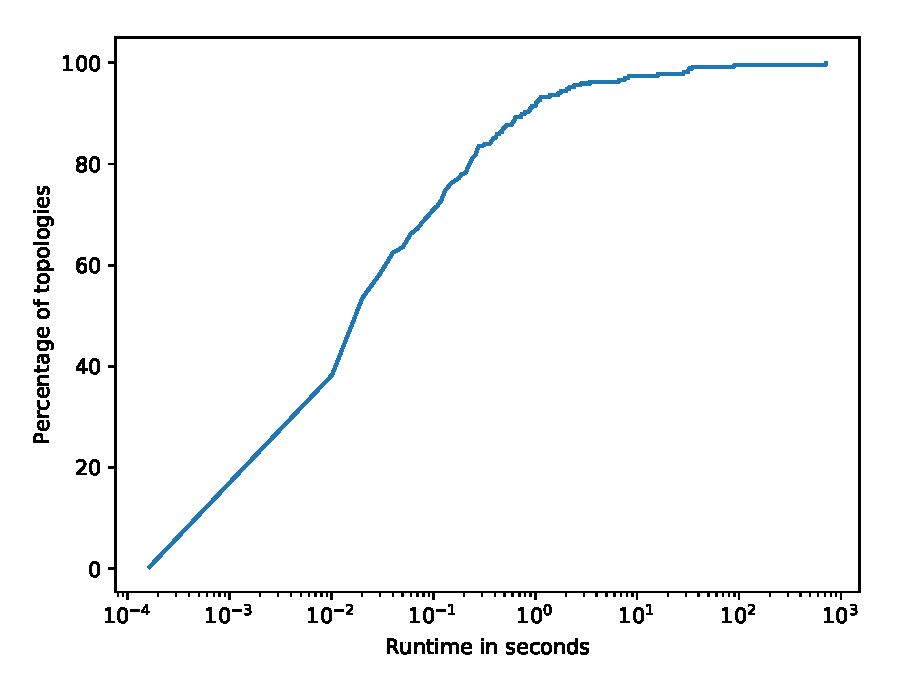
\includegraphics[width=.85\columnwidth]{./Network-lib/data/plot/minSegCover_runtime.eps}
\end{center}
\caption{Runtime CDF of Algorithm \ref{algo:min-seg-cover2} over all topologies.}
\label{fig:min-seg-cover-runtime}
\end{figure}

Figure \ref{fig:min-seg-cover-runtime-size} shows the runtime of ref{algo:min-seg-cover2} with respect to
the size of the topology $|G|$. We can observe that it indeed performs much better in practice than its theoretical
time complexity.

\begin{figure}
\begin{center}
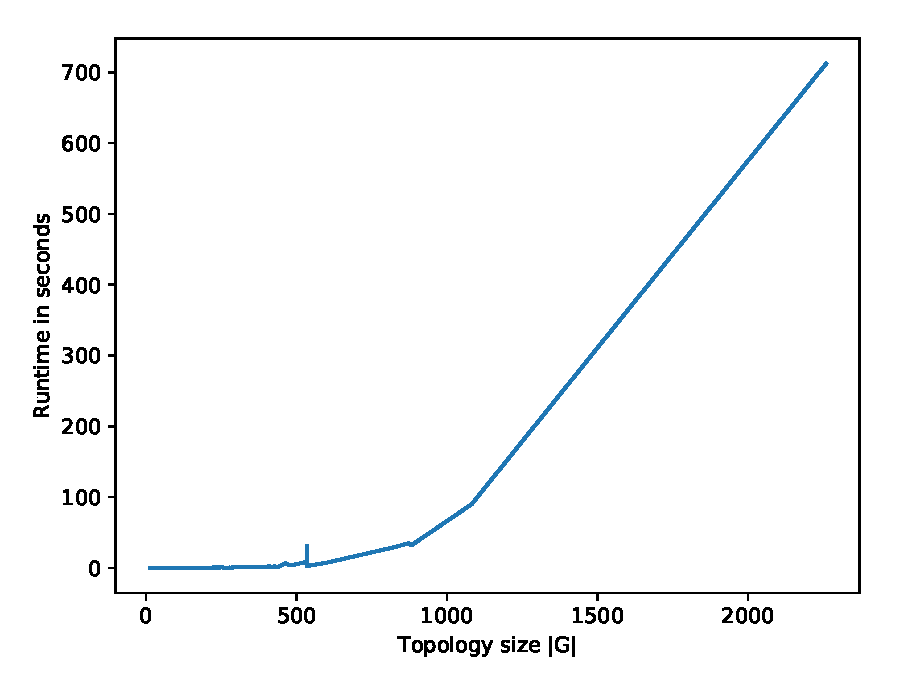
\includegraphics[width=.85\columnwidth]{./Network-lib/data/plot/minSegCover_runtime_by_size.eps}
\end{center}
\caption{Runtime by topology size of Algorithm \ref{algo:min-seg-cover2} over all topologies.}
\label{fig:min-seg-cover-runtime-size}
\end{figure}

Next, we analyze the segment cost of the sr-cycle covers produced by the algorithm. This gives a lower bound
on the segment cost of \emph{any} cycle cover on the given topologies. This is an important result as it shows
whether or not we can expect to be able to implement such a monitoring scheme on a segment routed network. As
we can see on Figure \ref{fig:min-seg-cover-segcost}, for more than $70\%$ we can find a cycle cover needing
at most a segment cost of $5$. This means that in most topologies such a sr-cycle cover is implementable even
on a network operating low end routers. Almost all topologies require a segment cost of at most $10$ showing
that network monitoring with segment routing is realistic for most topologies with high end routers. We wanted
to analyze the relationship between the size of the topology and the segment cost required for the sr-cycle cover.
The is shown in Figure \ref{fig:min-seg-cover-segcost-size}. We can see that the size does not seem to be 
correlated with the minimum segment cost.

\begin{figure}
\begin{center}
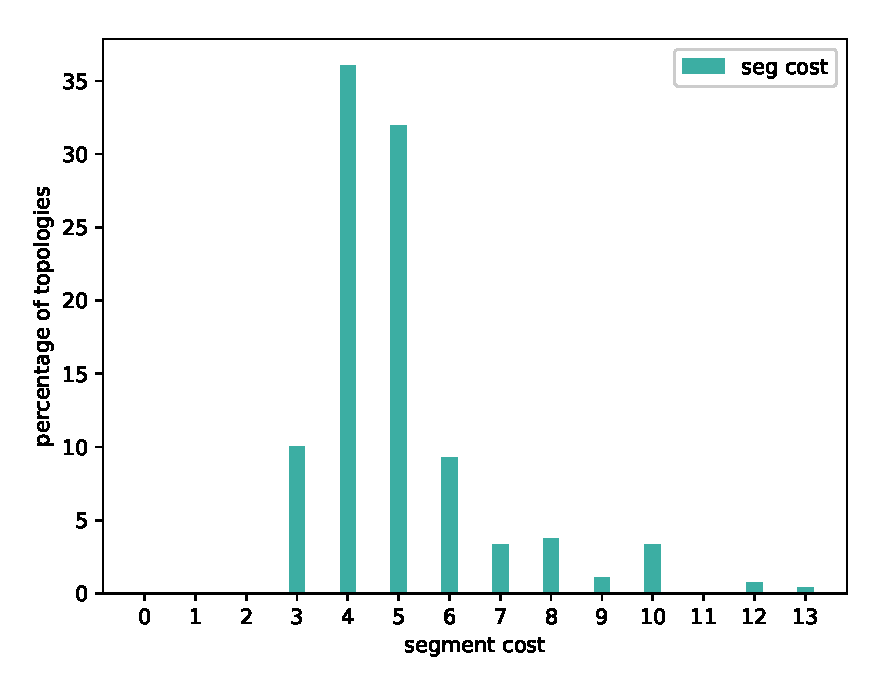
\includegraphics[width=.85\columnwidth]{./Network-lib/data/plot/minSegCover_segcost.eps}
\end{center}
\caption{Percentage of topologies for each segment cost.}
\label{fig:min-seg-cover-segcost}
\end{figure}


\begin{figure}
\begin{center}
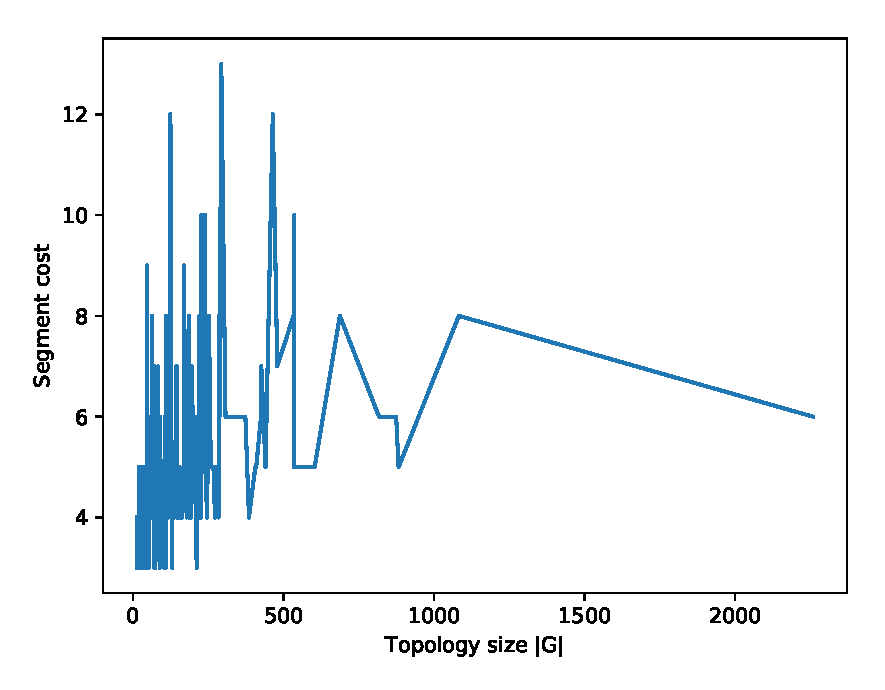
\includegraphics[width=.85\columnwidth]{./Network-lib/data/plot/minSegCover_segcost_by_size.eps}
\end{center}
\caption{Segment cost by topology size over all topologies.}
\label{fig:min-seg-cover-segcost-size}
\end{figure}


\section{Column generation cycle cover algorithm}

We saw in Chapter \ref{chapter:te} that column generation seemed to be a good framework to solve segment routing
problems. In this section we propose a column generation algorithm for computing lower bounds on the number of sr-cycles in a
minimum sr-cycle cover of a network. We also show how to derive from it an heuristic algorithm for Problem \ref{prob:min-cycle-cover}.

It is straightforward to express a MIP formulation for Problem \ref{prob:min-cycle-cover}. We define binary
variables $x_{\sr{c}}$ such that $x_{\sr{c}} = 1$ if and only if $\sr{c}$ is used in the cover. These variables
will be defined for every $\sr{c} \in \mathcal{C}^k_s$ where $k$ and $s$ are given as input. 

In terms of objective function, since we want to minimize the number of cycles in the cover, we can achieve this
by minimizing $\sum_{\sr{c} \in \mathcal{C}^k_s} x_{\sr{c}}$. This is so because this sum counts how many cycles
are used in the solution. For the constraints it is quite simple as well. We simply need to ensure that for each
edge $e \in E(G)$, there is at least one sr-cycle covering it, that is, there is at least one $\sr{c}$ such that
$x_{\sr{c}} = 1$ and $e \in E(\sr{c})$. We define the following identify function to simplify the expression of this constraints.

\begin{definition}
Given a network $G$ we define a function $I : \mathcal{P} \times E(G) \rightarrow \{0, 1\}$ such that
$I(\sr{p}, e) = 1$ if and only if $e \in E(\sr{p})$.
\end{definition}

\begin{center}
\begin{tabular}{crcllr}
\multicolumn{5}{l}{$\ccPrimalMip(G, k, s)$} \\[0.5cm] 
$\mathbf{min}$ & $\displaystyle \sum_{\sr{c} \in \mathcal{C}^k_s} x_{\sr{c}}$ & & & & \\[0.5cm]
$\textbf{s.t.}$ & $\displaystyle \sum_{\sr{c} \in \mathcal{C}^k_s} I(\sr{c}, e) \cdot x_{\sr{c}}$  & $\geq$ & $1$ & $\forall e \in E(G)$ & \\[0.5cm]
                & $x_{\sr{c}}$ & $\in$ & $\{0, 1\}$ & $\forall \sr{c} \in \mathcal{C}^k_s$
\end{tabular}
\end{center}

\subsection{Column generation}

We follow the same process that we did in Chapter \ref{chapter:te} to develop the column generation algorithm
for the minimum sr-cycle cover problem. Recall that CG is a technique for solving a LP and we have a MIP.
The first step is then to consider the LP-relaxation of $\ccPrimalMip$ and compute its dual.

\begin{center}
\begin{tabular}{crcllr}
\multicolumn{5}{l}{$\ccPrimalLp(G, k, s)$} \\[0.5cm] 
$\mathbf{min}$ & $\displaystyle \sum_{\sr{c} \in \mathcal{C}^k_s} x_{\sr{c}}$ & & & & \\[0.5cm]
$\textbf{s.t.}$ & $\displaystyle \sum_{\sr{c} \in \mathcal{C}^k_s} I(\sr{c}, e) \cdot x_{\sr{c}}$   & $\geq$ & $1$ & $\forall e \in E(G)$ & (P1) \\[0.5cm]
                & $x_{\sr{c}}$ & $\geq$  & $0$ & $\forall \sr{c} \in \mathcal{C}^k_s$
\end{tabular}
\end{center}

As before, the most natural relaxation would be to set $x_{\sr{c}} \in [0, 1]$ but our objective function guarantees that
this is equivalent to $x_{\sr{c}} \geq 0$. We chose the second one because it is equivalent and easier to work with.
The dual is obtained by following the same systematic procedure as before. By doing so we get the following LP.

\begin{center}
\begin{tabular}{crcllr}
\multicolumn{5}{l}{$\ccDualLp(G, k, s)$} \\[0.5cm] 
$\mathbf{max}$ & $\displaystyle \sum_{e \in E(G)} y_{e}$ & & & & \\[0.5cm]
$\textbf{s.t.}$ & $\displaystyle \sum_{e \in E(G)} I(\sr{c}, e) \cdot y_e$   & $\leq$ & $1$ & $\forall \sr{c} \in \mathcal{C}^k_s$ & (D1) \\[0.5cm]
                & $y_e$ & $\geq$ & $0$ & $\forall e \in E(G)$
\end{tabular}
\end{center}

The idea to solve $\ccPrimalLp$ is again to start with a small but feasible subset of sr-cycles $C \subseteq \mathcal{C}^k_s$ and 
slowly grow it until we can prove optimality. We denote the problems restricted to $C$ by adding $C$ as an argument, that is, by
$\ccPrimalLp(G, k, s, C)$ and $\ccDualLp(G, k, s, C)$. To find a new element $\sr{c}$ to add to $C$ we need to, given an optimal
solution $y^*$ of $\ccDualLp(G, k, s, C)$, find a sr-cycle $\sr{c}$ such that

$$
\sum_{e \in E(G)} I(\sr{c}, e) \cdot y^*_e = \sum_{e \in E(\sr{c})} y^*_e > 1.
$$

Solving this directly is \NPhard~since it can be shown to be equivalent to the longest path problem. 
Instead of trying to solve this pricing problem directly, we are going to see that by slightly changing the LP formulation we can
obtain a polynomial time solvable pricing problem.

\begin{definition}
Given a network $G$ we define a function $K : \mathcal{P} \times E(G) \rightarrow \mathbb{N}$ such that
$K(\sr{p}, e)$ equals the number of times $e$ is traversed by $\sr{p}$. Formally, if $\sr{p} = \langle x_1, \ldots, x_l \rangle$
$$
K(\sr{p}, e) = \sum_{i = 2}^l I(\sp(x^2_i, x^1_{i - 1}), e) + \sum_{i = 1 : x_i = e}^l 1.
$$
\end{definition}

By replacing $I$ by $K$ in the above formulations we still get a model for Problem \ref{prob:min-cycle-cover} since, the new constraints
corresponding to $(P1)$ with $I$ replaced by $K$, will still be true if and only if every edge is covered by at least one cycle. With this change the formulations become:

\begin{center}
\begin{tabular}{crcllr}
\multicolumn{5}{l}{$\ccPrimalLpK(G, k, s)$} \\[0.5cm] 
$\mathbf{min}$ & $\displaystyle \sum_{\sr{c} \in \mathcal{C}^k_s} x_{\sr{c}}$ & & & & \\[0.5cm]
$\textbf{s.t.}$ & $\displaystyle \sum_{\sr{c} \in \mathcal{C}^k_s} K(\sr{c}, e) \cdot x_{\sr{c}}$   & $\geq$ & $1$ & $\forall e \in E(G)$ &  \\[0.5cm]
                & $x_{\sr{c}}$ & $\geq$  & $0$ & $\forall \sr{c} \in \mathcal{C}^k_s$
\end{tabular}
\end{center}

\begin{center}
\begin{tabular}{crcllr}
\multicolumn{5}{l}{$\ccDualLpK(G, k, s)$} \\[0.5cm] 
$\mathbf{max}$ & $\displaystyle \sum_{e \in E(G)} y_{e}$ & & & & \\[0.5cm]
$\textbf{s.t.}$ & $\displaystyle \sum_{e \in E(G)} K(\sr{c}, e) \cdot y_e$   & $\leq$ & $1$ & $\forall \sr{c} \in \mathcal{C}^k_s$ &  \\[0.5cm]
                & $y_e$ & $\geq$ & $0$ & $\forall e \in E(G)$
\end{tabular}
\end{center}

The pricing problem now becomes the following one.

\begin{problem}{SRCC pricing}
\label{prob:cc-pricing}
\textbf{Input:} A network $G$, $k \in \mathbb{N}$, a source node $s \in V(G)$ and values $y_e \geq 0$ for each $e \in E(G)$.

\textbf{Output:} A sr-cycle $\sr{c} \in \mathcal{C}^k_s$ such that
$$
\sum_{e \in E(G)} K(\sr{c}, e) \cdot y_e > 1
$$
or report that no such sr-cycle exists.
\end{problem}

In order to solve Problem \ref{prob:cc-pricing}, we define a sr-metric $w$ such that 
$$
w(u, v) = \sum_{e \in \sp(u, v)} y_e
$$
and
$$
w(e) = y_e.
$$

With this metric, it is easy to see can see that
$$
w(\sr{c}) = \sum_{e \in E(G)} K(\sr{c}, e) \cdot y_e.
$$

Therefore we can solve the pricing problem by computing a sr-cycle $\sr{c}$ from $s$ to $s$ of segment
cost at most $k$ such that $w(\sr{c})$ is maximum. We have already shown in Chapter \ref{chapter:sr-optimal} that 
this problem can be solved in polynomial time. Therefore, we have the following theorem.

\begin{theorem}
Problem \ref{prob:cc-pricing} can be solved in polynomial time.
\end{theorem}

To start the column generation algorithm we need a feasible solution. In order to obtain one, we run Algorithm \ref{algo:min-seg-cover2} which also gives us
suitable source node $s$ and lower bound on the segment cost $k$. If the target segment cost is lower than $k$ then we immediately know
that a feasible solution does not exist. If it does, we use the cycles produced by the minimum segment cost cycle cover algorithm as an 
initial feasible solution for the column generation algorithm.

We evaluated the runtime of the column generation algorithm over all topologies. Figure \ref{fig:cc_runtime} shows a CDF of these runtimes.
The slowest topology took about $3$ hours so solve. Most topologies are solved in a very short amount of time and $98\%$ of the topologies
are solved in under $25$ minutes. These values are very reasonable given that the probing cycle only needs to be computed when the topology changes.

\begin{figure}
\begin{center}
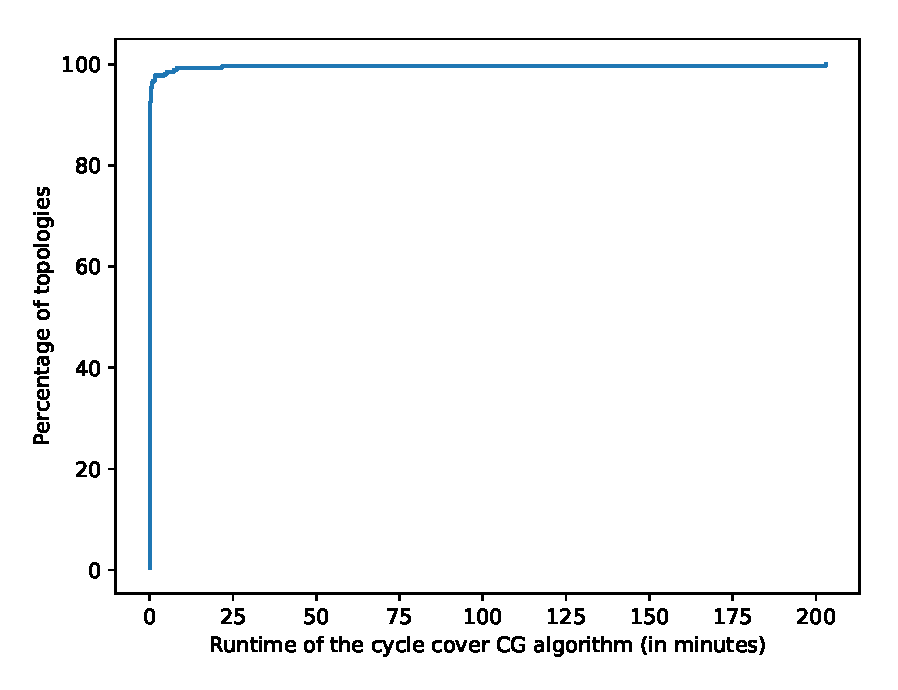
\includegraphics[width=.9\columnwidth]{./Network-lib/data/plot/minCycleCover_runtime_cdf.eps}
\end{center}
\caption{CDF of the runtime of the column generation cycle cover algorithm.}
\label{fig:cc_runtime}
\end{figure}

In the next section we will evaluate the lower bound provided by the column generation algorithm.


\subsection{Greedy algorithm}

We designed above a column generation algorithm for solving the LP relaxation of Problem \ref{prob:min-cycle-cover}. In this relaxation, an edge
can be covered fractionally by two sr-cycles or more. In this section we propose a greedy algorithm for converting these fractional solutions to proper 
solutions of Problem \ref{prob:min-cycle-cover}.

Let $C$ be the final set of sr-cycles. Our algorithm simply consists of selecting elements of $C$ 
while keeping track of the edges that are already covered until all of them are. At each step,
the sr-cycle that we selected is the sr-cycle that covers the maximum remaining uncovered edges. 

\begin{algorithm}[t]
\small
\caption{$\textsf{greedy-cc}\left( G, C \right)$}
\begin{algorithmic}[1]
%\algrule
\STATE $covered \gets \emptyset$
\STATE $cover \gets \emptyset$
\WHILE{$|U| < |E(G)|$}
  \STATE $\sr{c} \gets \sr{c} \in C \textbf{ such that } |E(\sr{c}) \cup covered| \textbf{ is maximum}$
  \STATE $cover \gets cover \cup \{ \sr{c} \}$
  \STATE $covered \gets covered \cup E(\sr{c})$
\ENDWHILE
\RETURN $cover$
\end{algorithmic}
\label{algo:greedy-cc}
\end{algorithm}

It is a well know result that this yields a logarithmic factor approximation. We prove this in the next theorem
for completeness.

\begin{theorem}
The set of cycles, $cover$, produced by Algorithm \ref{algo:greedy-cc} is such that
$$
opt_C \leq |cover| \leq \log|E(G)| \cdot opt_C
$$
where $opt_C$ is the size of a minimum over using only cycles from $C$.
\end{theorem}

\begin{proof}
Clearly, $opt_C \leq |cover|$. Let $m = |E(G)|$. 
Since the optimal solution relative to $C$ uses $opt_C$ sr-cycles, there must be at least one of them that covers at
least a fraction $1 \slash opt_C$ of the edges. If they were all below this ratio, they could not cover all edges.
Since we select the sr-cycle that covers the most uncovered edges, the first sr-cycle will cover
at least $1 \slash opt_C$ edges. Hence, after the first iteration, there are at most $m (1 - 1 \slash opt_C)$ edges left to cover. In the same way,
there must be a set that covers at least $1 \slash opt_C$ of these $m (1 - 1 \slash opt_C)$ edges. Since we select the 
sr-cycle covering the most edges, after the second iteration there are at most $m(1 - \slash opt_C)^2$ edges left. By repeating this argument,
we see that after $k$ iterations there are at most $m (1 - 1 \slash opt_C)^k$ edges left. Therefore, after $k = opt_C \log m$ iterations,
there are
$$
m (1 - 1 \slash opt_C)^{opt_C \log m} = m (1 \slash e)^{\log m} = m \cdot \frac{1}{e^{\log m}} = \frac{m}{m} = 1
$$
edges left. Hence $|cover| \leq \log m \cdot opt_C$.
\end{proof}

Ideally we would want to be able to prove that
$$
opt \leq |cover| \leq \log|E(G)| \cdot opt
$$
where $opt$ is the optimal solution over \emph{all} sr-cycles $\mathcal{C}^k_s$ but unfortunately this is not true in general.
However, since the fractional solution obtained with the column generation is a lower bound on $opt$ we can still evaluate how far
this gets us from the $opt$ in practice. Figure \ref{fig:sizes_3} shows the sizes of the minimum segment cost covers, the LP lower bound
and the sizes of the greedy covers.

\begin{figure}
\begin{center}
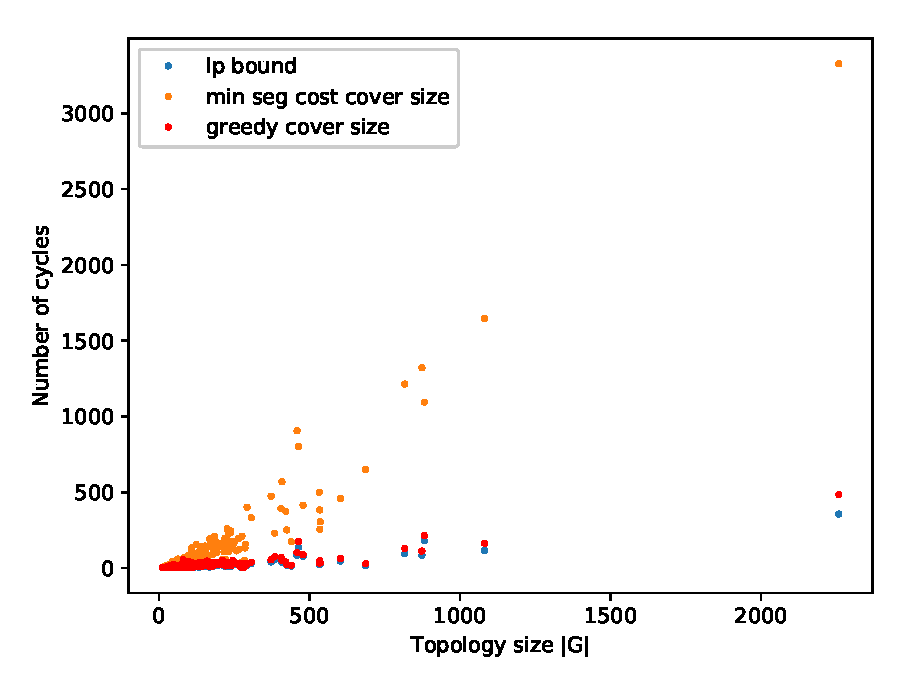
\includegraphics[width=.9\columnwidth]{./Network-lib/data/plot/minCycleCover_lowerbound.eps}
\end{center}
\caption{Lower bound, min seg cover size and greedy cover size shown by topologies size.}
\label{fig:sizes_3}
\end{figure}

We can see that the greedy solution is actually quite close to the lower bound and therefore it must also be
close to $opt$. To provide a better view of how close they are we computed a CDF of relative distance 
$$
\frac{greedy - lb}{lb}
$$
which is shown in Figure \ref{fig:cc_gap_cdf}. As a reference, with this metric, a value of $1$ 
means that the greedy solution uses twice the number of sr-cycle compared to the lower bound. 
We can see from the CDF that for $90\%$ of the instances we have an increase of at most
$50\%$ on the number of sr-cycles. Recall that this lower bound is not the actual number of sr-cycles in the optimal solution
but only an estimate. This means that our solution is actually even closer to the optimal solution.

\begin{figure}
\begin{center}
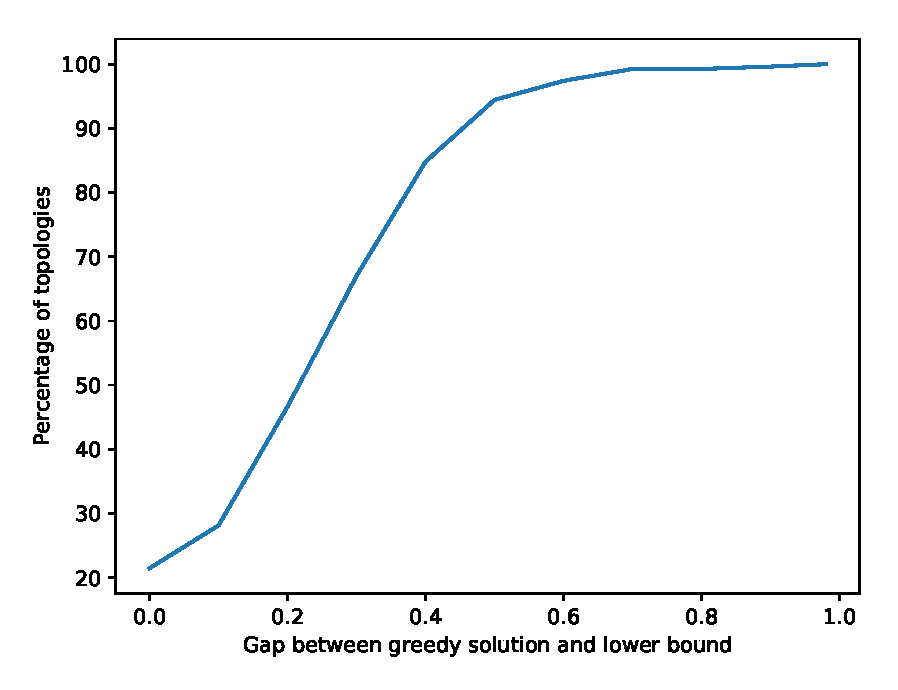
\includegraphics[width=.9\columnwidth]{./Network-lib/data/plot/minCycleCover_gapcdf.eps}
\end{center}
\caption{CDF of the gap between the greedy solution and the LP lower bound.}
\label{fig:cc_gap_cdf}
\end{figure}

The most important aspect is that by combining the minimum segment cost sr-cycle covers
with the column generation and the greedy algorithm we are able to greatly reduce the number of sr-cycles
in the minimum segment cost cover. Therefore, our solution is able to find sr-cycle covers that 
not only use the minimum amount of segments required for \emph{any} sr-cycle cover but also
are quite close to the minimum theoretical number of sr-cycles.


\section{Pinpointing single-link failures}

In this section we explain how to use a sr-cycle cover to detect single-link failures.

As mentioned in the introduction of this chapter, the idea is to have node $s$ 
regularly send monitoring probes over the sr-cycles of in a sr-cycle cover $C \subseteq \Csk$. Since we are using sr-cycles,
if the network is operating without failures, each probe must eventually come back to the vantage point $s$.
If at least one such probe does not come back, we know that at least one of the edges in the cycle associated with it
has a failure. We refer to the sr-cycles in the cycle cover $C$ as \emph{probing cycles}.

Let $\sr{c}$ be a cycle with a failure, that is, whose probe did not return. 
Because we use deterministic cycles, if we map $\sr{c}$ back to $G$, we get a cycle $c = (e_1, e_2, \ldots, e_l)$.
Recall that in this chapter we assume that the network $G$ is symmetric so that for each edge $e$ there is a reverse edge $\rev(e)$ and that
$\igp$ is symmetric if $\igp(e) = \rev(\igp(e))$.
The idea to detect the failure is to perform a binary search to find the largest $i$ such that
the cycle $c_i = (e_1, \ldots, e_i, \rev(e_i), \ldots, \rev(e_1))$ contains no failure. For each $i$ we send another 
probe over $c_i$ and check whether it comes back. If it does, then we know that the index we seek is greater than or equal to $i$. 
If it does not then the index must be strictly smaller than $i$. The single-link failure assumption is important for this process to work.
Because the probe did not cycle back, we know that one of 
$e_1, \ldots, e_l$ is faulty. Therefore, since we assume single-link
failure, we know that each reverse edge is not faulty. Hence, when we send a binary search probe on $c_i$, if it does not come back,
we know that the problem is in one of $e_1, \ldots, e_i$. We refer to these sr-cycles as \emph{identification cycles}.

Figure \ref{fig:bs-srcycle_new} illustrates this on an example with $l = 8$ and the failure is on edge $e_5$. We start the search with $i = 4$. The green dotted path
illustrates that the probe successfully returned to $v_1$. Thus we know that edges $e_1, e_2$ and $e_3$ are up.
The search will select $i = 6$ and this time the probe did not return. We conclude that the error is either in $e_4$ or $e_5$.
Finally, we send a probe on $c_5$ which returns. We finally conclude that the problem is on link $e_5$.

\begin{figure}
\begin{center}
\begin{tabular}{cc}
\begin{tikzpicture}[scale=0.75]
\node[scale=0.15] (a) at (3.000, 0.000) {\router{$v_1$}{router}};
\node[scale=0.15] (b) at (2.121, 2.121) {\router{$v_2$}{router}};
\node[scale=0.15] (c) at (0.000, 3.000) {\router{$v_3$}{router}};
\node[scale=0.15] (d) at (-2.121, 2.121) {\router{$v_4$}{router}};
\node[scale=0.15] (e) at (-3.000, 0.000) {\router{$v_5$}{router}};
\node[scale=0.15] (f) at (-2.121, -2.121) {\router{$v_6$}{router}};
\node[scale=0.15] (g) at (-0.000, -3.000) {\router{$v_7$}{router}};
\node[scale=0.15] (h) at (2.121, -2.121) {\router{$v_8$}{router}};

\draw[line width=2] (a) edge[above, sloped, bend right, ->] node[black,font=\bfseries] {\footnotesize \texttt{$e_1$}} (b);
\draw[line width=2] (b) edge[above, sloped, bend right, ->] node[black,font=\bfseries] {\footnotesize \texttt{$e_2$}} (c);
\draw[line width=2] (c) edge[above, sloped, bend right, ->] node[black,font=\bfseries] {\footnotesize \texttt{$e_3$}} (d);
\draw[line width=2] (d) edge[above, sloped, bend right, ->] node[black,font=\bfseries] {\footnotesize \texttt{$e_4$}} (e);
\draw[line width=2] (e) edge[below, sloped, bend right, ->] node[black,font=\bfseries] {\footnotesize \texttt{$e_5$}} (f);
\draw[line width=2] (f) edge[below, sloped, bend right, ->] node[black,font=\bfseries] {\footnotesize \texttt{$e_6$}} (g);
\draw[line width=2] (g) edge[below, sloped, bend right, ->] node[black,font=\bfseries] {\footnotesize \texttt{$e_7$}} (h);
\draw[line width=2] (h) edge[below, sloped, bend right, ->] node[black,font=\bfseries] {\footnotesize \texttt{$e_8$}} (a);
\draw (e) edge[sloped, bend right, ->] node[red, font=\bfseries] {\footnotesize \texttt{\Large \textsf{X}}} (f);

\draw[line width=2, gray] (a) edge[below, sloped, bend left, <-] node[gray,font=\bfseries] {\footnotesize \texttt{$\rev(e_1)$}} (b);
\draw[line width=2, gray] (b) edge[below, sloped, bend left, <-] node[gray,font=\bfseries] {\footnotesize \texttt{$\rev(e_2)$}} (c);
\draw[line width=2, gray] (c) edge[below, sloped, bend left, <-] node[gray,font=\bfseries] {\footnotesize \texttt{$\rev(e_3)$}} (d);
\draw[line width=2, gray] (d) edge[below, sloped, bend left, <-] node[gray,font=\bfseries] {\footnotesize \texttt{$\rev(e_4)$}} (e);
\draw[line width=2, gray] (e) edge[above, sloped, bend left, <-] node[gray,font=\bfseries] {\footnotesize \texttt{$\rev(e_5)$}} (f);

\draw[line width=2, gray] (f) edge[above, sloped, bend left, <-] node[gray,font=\bfseries] {\footnotesize \texttt{$\rev(e_6)$}} (g);
\draw[line width=2, gray] (g) edge[above, sloped, bend left, <-] node[gray,font=\bfseries] {\footnotesize \texttt{$\rev(e_7)$}} (h);
\draw[line width=2, gray] (h) edge[above, sloped, bend left, <-] node[gray,font=\bfseries] {\footnotesize \texttt{$\rev(e_8)$}} (a);

\draw[darkgreen, ultra thick, dotted, ->] plot [smooth] coordinates { ($(a)+(0.5,0)$) ($(b)+(0,0.5)$) ($(c)+(0,0.5)$) ($(d)+(0,0.5)$) ($(d)+(-0.5,0)$) ($(d)+(0,-0.5)$) ($(c)+(0,-0.5)$) ($(b)+(0,-0.5)$) ($(a)$) };

\end{tikzpicture}

&

\begin{tikzpicture}[scale=0.75]
\node[scale=0.15] (1) at (3.000, 0.000) {\router{$v_1$}{router}};
\node[scale=0.15] (2) at (2.121, 2.121) {\router{$v_2$}{router}};
\node[scale=0.15] (3) at (0.000, 3.000) {\router{$v_3$}{router}};
\node[scale=0.15] (4) at (-2.121, 2.121) {\router{$v_4$}{green}};
\node[scale=0.15] (5) at (-3.000, 0.000) {\router{$v_5$}{router}};
\node[scale=0.15] (6) at (-2.121, -2.121) {\router{$v_6$}{router}};
\node[scale=0.15] (7) at (-0.000, -3.000) {\router{$v_7$}{router}};
\node[scale=0.15] (8) at (2.121, -2.121) {\router{$v_8$}{router}};

\draw[line width=2, darkgreen] (1) edge[above, sloped, bend right, ->] node[black,font=\bfseries] {\footnotesize \texttt{$e_1$}} (2);
\draw[line width=2, darkgreen] (2) edge[above, sloped, bend right, ->] node[black,font=\bfseries] {\footnotesize \texttt{$e_2$}} (3);
\draw[line width=2, darkgreen] (3) edge[above, sloped, bend right, ->] node[black,font=\bfseries] {\footnotesize \texttt{$e_3$}} (4);
\draw[line width=2] (4) edge[above, sloped, bend right, ->] node[black,font=\bfseries] {\footnotesize \texttt{$e_4$}} (5);
\draw[line width=2] (5) edge[below, sloped, bend right, ->] node[black,font=\bfseries] {\footnotesize \texttt{$e_5$}} (6);
\draw[line width=2] (6) edge[below, sloped, bend right, ->] node[black,font=\bfseries] {\footnotesize \texttt{$e_6$}} (7);
\draw[line width=2] (7) edge[below, sloped, bend right, ->] node[black,font=\bfseries] {\footnotesize \texttt{$e_7$}} (8);
\draw[line width=2] (8) edge[below, sloped, bend right, ->] node[black,font=\bfseries] {\footnotesize \texttt{$e_8$}} (1);
\draw (5) edge[sloped, bend right, ->] node[red, font=\bfseries] {\footnotesize \texttt{\Large \textsf{X}}} (6);

\draw[line width=2, gray, darkgreen] (1) edge[below, sloped, bend left, <-] node[gray,font=\bfseries] {\footnotesize \texttt{$\rev(e_1)$}} (2);
\draw[line width=2, gray, darkgreen] (2) edge[below, sloped, bend left, <-] node[gray,font=\bfseries] {\footnotesize \texttt{$\rev(e_2)$}} (3);
\draw[line width=2, gray, darkgreen] (3) edge[below, sloped, bend left, <-] node[gray,font=\bfseries] {\footnotesize \texttt{$\rev(e_3)$}} (4);
\draw[line width=2, gray] (4) edge[below, sloped, bend left, <-] node[gray,font=\bfseries] {\footnotesize \texttt{$\rev(e_4)$}} (5);
\draw[line width=2, gray] (5) edge[above, sloped, bend left, <-] node[gray,font=\bfseries] {\footnotesize \texttt{$\rev(e_5)$}} (6);
\draw[line width=2, gray] (6) edge[above, sloped, bend left, <-] node[gray,font=\bfseries] {\footnotesize \texttt{$\rev(e_6)$}} (7);
\draw[line width=2, gray] (7) edge[above, sloped, bend left, <-] node[gray,font=\bfseries] {\footnotesize \texttt{$\rev(e_7)$}} (8);
\draw[line width=2, gray] (8) edge[above, sloped, bend left, <-] node[gray,font=\bfseries] {\footnotesize \texttt{$\rev(e_8)$}} (1);

\draw[red!50!black, ultra thick, dotted, ->] plot [smooth] coordinates { 
($(a)+(0.5,0)$) ($(b)+(0,0.5)$) ($(c)+(0,0.5)$) ($(d)+(0,0.5)$) ($(e)+(-0.5,0)$) ($(f)+(-0.5,0)$) 
($(f)+(0,-0.5)$) ($(f)+(0.5,0)$) ($(e)+(0.5,0)$) ($(d)+(0,-0.5)$) ($(c)+(0,-0.5)$) ($(b)+(0,-0.5)$) ($(a)$) 
};

\end{tikzpicture}

\\

\footnotesize

First step of binary search. Success.

&

\footnotesize

Second step of binary search. Failure.

\\

\footnotesize

Edges $e_1, e_2, e_3$ are up.

&

\footnotesize

One of $e_4, e_5$ is down.

\\[0.5cm]

\begin{tikzpicture}[scale=0.75]
\node[scale=0.15] (1) at (3.000, 0.000) {\router{$v_1$}{router}};
\node[scale=0.15] (2) at (2.121, 2.121) {\router{$v_2$}{router}};
\node[scale=0.15] (3) at (0.000, 3.000) {\router{$v_3$}{router}};
\node[scale=0.15] (4) at (-2.121, 2.121) {\router{$v_4$}{green}};
\node[scale=0.15] (5) at (-3.000, 0.000) {\router{$v_5$}{router}};
\node[scale=0.15] (6) at (-2.121, -2.121) {\router{$v_6$}{red!50!white}};
\node[scale=0.15] (7) at (-0.000, -3.000) {\router{$v_7$}{router}};
\node[scale=0.15] (8) at (2.121, -2.121) {\router{$v_8$}{router}};

\draw[line width=2, darkgreen] (1) edge[above, sloped, bend right, ->] node[black,font=\bfseries] {\footnotesize \texttt{$e_1$}} (2);
\draw[line width=2, darkgreen] (2) edge[above, sloped, bend right, ->] node[black,font=\bfseries] {\footnotesize \texttt{$e_2$}} (3);
\draw[line width=2, darkgreen] (3) edge[above, sloped, bend right, ->] node[black,font=\bfseries] {\footnotesize \texttt{$e_3$}} (4);
\draw[line width=2] (4) edge[above, sloped, bend right, ->] node[black,font=\bfseries] {\footnotesize \texttt{$e_4$}} (5);
\draw[line width=2] (5) edge[below, sloped, bend right, ->] node[black,font=\bfseries] {\footnotesize \texttt{$e_5$}} (6);
\draw[line width=2] (6) edge[below, sloped, bend right, ->] node[black,font=\bfseries] {\footnotesize \texttt{$e_6$}} (7);
\draw[line width=2] (7) edge[below, sloped, bend right, ->] node[black,font=\bfseries] {\footnotesize \texttt{$e_7$}} (8);
\draw[line width=2] (8) edge[below, sloped, bend right, ->] node[black,font=\bfseries] {\footnotesize \texttt{$e_8$}} (1);
\draw (5) edge[sloped, bend right, ->] node[red, font=\bfseries] {\footnotesize \texttt{\Large \textsf{X}}} (6);

\draw[line width=2, gray, darkgreen] (1) edge[below, sloped, bend left, <-] node[gray,font=\bfseries] {\footnotesize \texttt{$\rev(e_1)$}} (2);
\draw[line width=2, gray, darkgreen] (2) edge[below, sloped, bend left, <-] node[gray,font=\bfseries] {\footnotesize \texttt{$\rev(e_2)$}} (3);
\draw[line width=2, gray, darkgreen] (3) edge[below, sloped, bend left, <-] node[gray,font=\bfseries] {\footnotesize \texttt{$\rev(e_3)$}} (4);
\draw[line width=2, gray] (4) edge[below, sloped, bend left, <-] node[gray,font=\bfseries] {\footnotesize \texttt{$\rev(e_4)$}} (5);
\draw[line width=2, gray] (5) edge[above, sloped, bend left, <-] node[gray,font=\bfseries] {\footnotesize \texttt{$\rev(e_5)$}} (6);
\draw[line width=2, gray] (6) edge[above, sloped, bend left, <-] node[gray,font=\bfseries] {\footnotesize \texttt{$\rev(e_6)$}} (7);
\draw[line width=2, gray] (7) edge[above, sloped, bend left, <-] node[gray,font=\bfseries] {\footnotesize \texttt{$\rev(e_7)$}} (8);
\draw[line width=2, gray] (8) edge[above, sloped, bend left, <-] node[gray,font=\bfseries] {\footnotesize \texttt{$\rev(e_8)$}} (1);

\draw[darkgreen, ultra thick, dotted, ->] plot [smooth] coordinates { 
($(a)+(0.5,0)$) ($(b)+(0,0.5)$) ($(c)+(0,0.5)$) ($(d)+(0,0.5)$) ($(e)+(-0.5,0)$) 
($(e)+(0,-0.5)$) ($(e)+(0.5,0)$) ($(d)+(0,-0.5)$) ($(c)+(0,-0.5)$) ($(b)+(0,-0.5)$) ($(a)$) 
};

\end{tikzpicture}

&


\begin{tikzpicture}[scale=0.75]
\node[scale=0.15] (1) at (3.000, 0.000) {\router{$v_1$}{router}};
\node[scale=0.15] (2) at (2.121, 2.121) {\router{$v_2$}{router}};
\node[scale=0.15] (3) at (0.000, 3.000) {\router{$v_3$}{router}};
\node[scale=0.15] (4) at (-2.121, 2.121) {\router{$v_4$}{green}};
\node[scale=0.15] (5) at (-3.000, 0.000) {\router{$v_5$}{green}};
\node[scale=0.15] (6) at (-2.121, -2.121) {\router{$v_6$}{red!50!white}};
\node[scale=0.15] (7) at (-0.000, -3.000) {\router{$v_7$}{router}};
\node[scale=0.15] (8) at (2.121, -2.121) {\router{$v_8$}{router}};

\draw[line width=2, darkgreen] (1) edge[above, sloped, bend right, ->] node[black,font=\bfseries] {\footnotesize \texttt{$e_1$}} (2);
\draw[line width=2, darkgreen] (2) edge[above, sloped, bend right, ->] node[black,font=\bfseries] {\footnotesize \texttt{$e_2$}} (3);
\draw[line width=2, darkgreen] (3) edge[above, sloped, bend right, ->] node[black,font=\bfseries] {\footnotesize \texttt{$e_3$}} (4);
\draw[line width=2, darkgreen] (4) edge[above, sloped, bend right, ->] node[black,font=\bfseries] {\footnotesize \texttt{$e_4$}} (5);
\draw[line width=2] (5) edge[below, red!50!black, sloped, bend right, ->] node[black,font=\bfseries] {\footnotesize \texttt{$e_5$}} (6);
\draw[line width=2, opacity=0] (5) edge[red!50!black, sloped, bend right, ->] node (e5) {} (6);
\draw (5) edge[sloped, bend right, ->] node[red, font=\bfseries] {\footnotesize \texttt{\Large \textsf{X}}} (6);

\draw[line width=2] (6) edge[below, sloped, bend right, ->] node[black,font=\bfseries] {\footnotesize \texttt{$e_6$}} (7);
\draw[line width=2] (7) edge[below, sloped, bend right, ->] node[black,font=\bfseries] {\footnotesize \texttt{$e_7$}} (8);
\draw[line width=2] (8) edge[below, sloped, bend right, ->] node[black,font=\bfseries] {\footnotesize \texttt{$e_8$}} (1);

\draw[line width=2, gray, darkgreen] (1) edge[below, sloped, bend left, <-] node[gray,font=\bfseries] {\footnotesize \texttt{$\rev(e_1)$}} (2);
\draw[line width=2, gray, darkgreen] (2) edge[below, sloped, bend left, <-] node[gray,font=\bfseries] {\footnotesize \texttt{$\rev(e_2)$}} (3);
\draw[line width=2, gray, darkgreen] (3) edge[below, sloped, bend left, <-] node[gray,font=\bfseries] {\footnotesize \texttt{$\rev(e_3)$}} (4);
\draw[line width=2, gray, darkgreen] (4) edge[below, sloped, bend left, <-] node[gray,font=\bfseries] {\footnotesize \texttt{$\rev(e_4)$}} (5);
\draw[line width=2, gray, gray] (5) edge[above, sloped, bend left, <-] node[gray,font=\bfseries] {\footnotesize \texttt{$\rev(e_5)$}} (6);
%\draw[line width=2, gray, red!50!black, opacity=0] (5) edge[sloped, bend left, <-] node[gray,font=\bfseries] (re5) {} (6);


\draw[line width=2, gray] (6) edge[above, sloped, bend left, <-] node[gray,font=\bfseries] {\footnotesize \texttt{$\rev(e_6)$}} (7);
\draw[line width=2, gray] (7) edge[above, sloped, bend left, <-] node[gray,font=\bfseries] {\footnotesize \texttt{$\rev(e_7)$}} (8);
\draw[line width=2, gray] (8) edge[above, sloped, bend left, <-] node[gray,font=\bfseries] {\footnotesize \texttt{$\rev(e_8)$}} (1);

%\draw[darkgreen, ultra thick, dotted, ->] plot [smooth] coordinates { 
%($(a)+(0.5,0)$) ($(b)+(0,0.5)$) ($(c)+(0,0.5)$) ($(d)+(0,0.5)$) ($(e)+(-0.5,0)$) 
%($(e)+(0,-0.5)$) ($(e)+(0.5,0)$) ($(d)+(0,-0.5)$) ($(c)+(0,-0.5)$) ($(b)+(0,-0.5)$) ($(a)$) 
%};

%\node (fail) at (0, 0) {failure};

%\draw[->, dashed] (fail) -- (e5);
%\draw[->, dashed] (fail) -- (re5);


\end{tikzpicture}

\\

\footnotesize

Third step of binary search. Success.

&

\footnotesize

End of the search.

\\

\footnotesize

Edges $e_4$ is up.

&

\footnotesize

Failure detected in $e_5$.

\end{tabular}
\end{center}
\caption{Binary search to identify the failure (single-link failure assumption).}
\label{fig:bs-srcycle_new}
\end{figure}

To illustrate why the single link-failure assumption is important, let's see happens with this process
when multiple failures occur. Imagine the same example as in Figure \ref{fig:bs-srcycle_new} but assume that
edge $\rev(e_3)$ is also down. In this case the first binary search probe will fail to return and the search
will stop at $i = 3$ and the algorithm will say that the problem is on edge $e_3$. However $e_3$ is up
and it is $\rev(e_3)$ that prevents the probe to return. This shows that with multiple failures, we cannot
know exactly which link is down. However, we still can say that either $e_3$ is down \emph{or} $\rev(e_3)$ is
down. Figure \ref{fig:bs-srcycle_new2} illustrates this.

This means that in presence of multiple link failures, we cannot tell exactly which link is down but we can
still find a set of two links $\{ e, \rev(e) \}$ such that we are sure that at least one of them is down.

\begin{figure}
\begin{center}
\begin{tabular}{cc}
\begin{tikzpicture}[scale=0.75]
\node[scale=0.15] (a) at (3.000, 0.000) {\router{$v_1$}{router}};
\node[scale=0.15] (b) at (2.121, 2.121) {\router{$v_2$}{router}};
\node[scale=0.15] (c) at (0.000, 3.000) {\router{$v_3$}{router}};
\node[scale=0.15] (d) at (-2.121, 2.121) {\router{$v_4$}{router}};
\node[scale=0.15] (e) at (-3.000, 0.000) {\router{$v_5$}{router}};
\node[scale=0.15] (f) at (-2.121, -2.121) {\router{$v_6$}{router}};
\node[scale=0.15] (g) at (-0.000, -3.000) {\router{$v_7$}{router}};
\node[scale=0.15] (h) at (2.121, -2.121) {\router{$v_8$}{router}};

\draw[line width=2] (a) edge[above, sloped, bend right, ->] node[black,font=\bfseries] {\footnotesize \texttt{$e_1$}} (b);
\draw[line width=2] (b) edge[above, sloped, bend right, ->] node[black,font=\bfseries] {\footnotesize \texttt{$e_2$}} (c);
\draw[line width=2] (c) edge[above, sloped, bend right, ->] node[black,font=\bfseries] {\footnotesize \texttt{$e_3$}} (d);
\draw[line width=2] (d) edge[above, sloped, bend right, ->] node[black,font=\bfseries] {\footnotesize \texttt{$e_4$}} (e);
\draw[line width=2] (e) edge[below, sloped, bend right, ->] node[black,font=\bfseries] {\footnotesize \texttt{$e_5$}} (f);
\draw[line width=2] (f) edge[below, sloped, bend right, ->] node[black,font=\bfseries] {\footnotesize \texttt{$e_6$}} (g);
\draw[line width=2] (g) edge[below, sloped, bend right, ->] node[black,font=\bfseries] {\footnotesize \texttt{$e_7$}} (h);
\draw[line width=2] (h) edge[below, sloped, bend right, ->] node[black,font=\bfseries] {\footnotesize \texttt{$e_8$}} (a);
\draw (e) edge[sloped, bend right, ->] node[red, font=\bfseries] {\Large \textsf{X}} (f);

\draw[line width=2, gray] (a) edge[below, sloped, bend left, <-] node[gray,font=\bfseries] {\footnotesize \texttt{$\rev(e_1)$}} (b);
\draw[line width=2, gray] (b) edge[below, sloped, bend left, <-] node[gray,font=\bfseries] {\footnotesize \texttt{$\rev(e_2)$}} (c);
\draw[line width=2, gray] (c) edge[below, sloped, bend left, <-] node[gray,font=\bfseries] {\footnotesize \texttt{$\rev(e_3)$}} (d);
\draw[line width=2, gray] (d) edge[below, sloped, bend left, <-] node[gray,font=\bfseries] {\footnotesize \texttt{$\rev(e_4)$}} (e);
\draw[line width=2, gray] (e) edge[above, sloped, bend left, <-] node[gray,font=\bfseries] {\footnotesize \texttt{$\rev(e_5)$}} (f);
\draw[line width=2, gray] (c) edge[sloped, bend left, <-] node[red,font=\bfseries] {\Large \textsf{X}} (d);

\draw[line width=2, gray] (f) edge[above, sloped, bend left, <-] node[gray,font=\bfseries] {\footnotesize \texttt{$\rev(e_6)$}} (g);
\draw[line width=2, gray] (g) edge[above, sloped, bend left, <-] node[gray,font=\bfseries] {\footnotesize \texttt{$\rev(e_7)$}} (h);
\draw[line width=2, gray] (h) edge[above, sloped, bend left, <-] node[gray,font=\bfseries] {\footnotesize \texttt{$\rev(e_8)$}} (a);

\draw[red!50!black, ultra thick, dotted, ->] plot [smooth] coordinates { ($(a)+(0.5,0)$) ($(b)+(0,0.5)$) ($(c)+(0,0.5)$) ($(d)+(0,0.5)$) ($(d)+(-0.5,0)$) ($(d)+(0,-0.5)$) ($(c)+(0,-0.5)$) ($(b)+(0,-0.5)$) ($(a)$) };

\end{tikzpicture}

&

\begin{tikzpicture}[scale=0.75]
\node[scale=0.15] (1) at (3.000, 0.000) {\router{$v_1$}{router}};
\node[scale=0.15] (2) at (2.121, 2.121) {\router{$v_2$}{router}};
\node[scale=0.15] (3) at (0.000, 3.000) {\router{$v_3$}{router}};
\node[scale=0.15] (4) at (-2.121, 2.121) {\router{$v_4$}{red!50!white}};
\node[scale=0.15] (5) at (-3.000, 0.000) {\router{$v_5$}{router}};
\node[scale=0.15] (6) at (-2.121, -2.121) {\router{$v_6$}{router}};
\node[scale=0.15] (7) at (-0.000, -3.000) {\router{$v_7$}{router}};
\node[scale=0.15] (8) at (2.121, -2.121) {\router{$v_8$}{router}};

\draw[line width=2] (1) edge[above, sloped, bend right, ->] node[black,font=\bfseries] {\footnotesize \texttt{$e_1$}} (2);
\draw[line width=2] (2) edge[above, sloped, bend right, ->] node[black,font=\bfseries] {\footnotesize \texttt{$e_2$}} (3);
\draw[line width=2] (3) edge[above, sloped, bend right, ->] node[black,font=\bfseries] {\footnotesize \texttt{$e_3$}} (4);
\draw[line width=2] (4) edge[above, sloped, bend right, ->] node[black,font=\bfseries] {\footnotesize \texttt{$e_4$}} (5);
\draw[line width=2] (5) edge[below, sloped, bend right, ->] node[black,font=\bfseries] {\footnotesize \texttt{$e_5$}} (6);
\draw[line width=2] (6) edge[below, sloped, bend right, ->] node[black,font=\bfseries] {\footnotesize \texttt{$e_6$}} (7);
\draw[line width=2] (7) edge[below, sloped, bend right, ->] node[black,font=\bfseries] {\footnotesize \texttt{$e_7$}} (8);
\draw[line width=2] (8) edge[below, sloped, bend right, ->] node[black,font=\bfseries] {\footnotesize \texttt{$e_8$}} (1);
\draw (5) edge[sloped, bend right, ->] node[red, font=\bfseries] {\footnotesize \texttt{\Large \textsf{X}}} (6);

\draw[line width=2, gray] (1) edge[below, sloped, bend left, <-] node[gray,font=\bfseries] {\footnotesize \texttt{$\rev(e_1)$}} (2);
\draw[line width=2, gray] (2) edge[below, sloped, bend left, <-] node[gray,font=\bfseries] {\footnotesize \texttt{$\rev(e_2)$}} (3);
\draw[line width=2, gray] (3) edge[below, sloped, bend left, <-] node[gray,font=\bfseries] {\footnotesize \texttt{$\rev(e_3)$}} (4);
\draw[line width=2, gray] (4) edge[below, sloped, bend left, <-] node[gray,font=\bfseries] {\footnotesize \texttt{$\rev(e_4)$}} (5);
\draw[line width=2, gray] (5) edge[above, sloped, bend left, <-] node[gray,font=\bfseries] {\footnotesize \texttt{$\rev(e_5)$}} (6);
\draw[line width=2, gray] (6) edge[above, sloped, bend left, <-] node[gray,font=\bfseries] {\footnotesize \texttt{$\rev(e_6)$}} (7);
\draw[line width=2, gray] (7) edge[above, sloped, bend left, <-] node[gray,font=\bfseries] {\footnotesize \texttt{$\rev(e_7)$}} (8);
\draw[line width=2, gray] (8) edge[above, sloped, bend left, <-] node[gray,font=\bfseries] {\footnotesize \texttt{$\rev(e_8)$}} (1);
\draw[line width=2, gray] (c) edge[sloped, bend left, <-] node[red,font=\bfseries] {\Large \textsf{X}} (d);

\draw[darkgreen, ultra thick, dotted, ->] plot [smooth] coordinates 
{ ($(a)+(0.5,0)$) ($(b)+(0.5,0.5)$) ($(b)+(0,0.5)$) ($(b)+(-0.5,0)$)($(a)$) };

\end{tikzpicture}

\\

\footnotesize

First step of binary search. Failure.

&

\footnotesize

Second step of binary search. Success.

\\

\footnotesize

One of $e_1, e_2, e_3, \rev(e_3), \rev(e_2), \rev(e_1)$ is down.

&

\footnotesize

Edges $e_1, \rev(e_1)$ are up.

\\[0.5cm]

\begin{tikzpicture}[scale=0.75]
\node[scale=0.15] (1) at (3.000, 0.000) {\router{$v_1$}{router}};
\node[scale=0.15] (2) at (2.121, 2.121) {\router{$v_2$}{green}};
\node[scale=0.15] (3) at (0.000, 3.000) {\router{$v_3$}{router}};
\node[scale=0.15] (4) at (-2.121, 2.121) {\router{$v_4$}{red!50!white}};
\node[scale=0.15] (5) at (-3.000, 0.000) {\router{$v_5$}{router}};
\node[scale=0.15] (6) at (-2.121, -2.121) {\router{$v_6$}{router}};
\node[scale=0.15] (7) at (-0.000, -3.000) {\router{$v_7$}{router}};
\node[scale=0.15] (8) at (2.121, -2.121) {\router{$v_8$}{router}};

\draw[line width=2] (1) edge[darkgreen, sloped, bend right, ->] node[black,font=\bfseries] {\footnotesize \texttt{$e_1$}} (2);
\draw[line width=2] (2) edge[above, sloped, bend right, ->] node[black,font=\bfseries] {\footnotesize \texttt{$e_2$}} (3);
\draw[line width=2] (3) edge[above, sloped, bend right, ->] node[black,font=\bfseries] {\footnotesize \texttt{$e_3$}} (4);
\draw[line width=2] (4) edge[above, sloped, bend right, ->] node[black,font=\bfseries] {\footnotesize \texttt{$e_4$}} (5);
\draw[line width=2] (5) edge[below, sloped, bend right, ->] node[black,font=\bfseries] {\footnotesize \texttt{$e_5$}} (6);
\draw[line width=2] (6) edge[below, sloped, bend right, ->] node[black,font=\bfseries] {\footnotesize \texttt{$e_6$}} (7);
\draw[line width=2] (7) edge[below, sloped, bend right, ->] node[black,font=\bfseries] {\footnotesize \texttt{$e_7$}} (8);
\draw[line width=2] (8) edge[below, sloped, bend right, ->] node[black,font=\bfseries] {\footnotesize \texttt{$e_8$}} (1);
\draw (5) edge[sloped, bend right, ->] node[red, font=\bfseries] {\footnotesize \texttt{\Large \textsf{X}}} (6);

\draw[line width=2, gray] (1) edge[darkgreen, below, sloped, bend left, <-] node[gray,font=\bfseries] {\footnotesize \texttt{$\rev(e_1)$}} (2);
\draw[line width=2, gray] (2) edge[below, sloped, bend left, <-] node[gray,font=\bfseries] {\footnotesize \texttt{$\rev(e_2)$}} (3);
\draw[line width=2, gray] (3) edge[below, sloped, bend left, <-] node[gray,font=\bfseries] {\footnotesize \texttt{$\rev(e_3)$}} (4);
\draw[line width=2, gray] (4) edge[below, sloped, bend left, <-] node[gray,font=\bfseries] {\footnotesize \texttt{$\rev(e_4)$}} (5);
\draw[line width=2, gray] (5) edge[above, sloped, bend left, <-] node[gray,font=\bfseries] {\footnotesize \texttt{$\rev(e_5)$}} (6);
\draw[line width=2, gray] (6) edge[above, sloped, bend left, <-] node[gray,font=\bfseries] {\footnotesize \texttt{$\rev(e_6)$}} (7);
\draw[line width=2, gray] (7) edge[above, sloped, bend left, <-] node[gray,font=\bfseries] {\footnotesize \texttt{$\rev(e_7)$}} (8);
\draw[line width=2, gray] (8) edge[above, sloped, bend left, <-] node[gray,font=\bfseries] {\footnotesize \texttt{$\rev(e_8)$}} (1);
\draw[line width=2, gray] (c) edge[sloped, bend left, <-] node[red,font=\bfseries] {\Large \textsf{X}} (d);

\draw[darkgreen, ultra thick, dotted, ->] plot [smooth] coordinates 
{ ($(a)+(0.5,0)$) ($(b)+(0,0.5)$) ($(c)+(0,0.5)$) ($(c)+(-0.5,0)$) ($(c)+(0,-0.5)$) ($(b)+(0,-0.5)$) ($(a)$) };

\end{tikzpicture}


&


\begin{tikzpicture}[scale=0.75]
\node[scale=0.15] (1) at (3.000, 0.000) {\router{$v_1$}{router}};
\node[scale=0.15] (2) at (2.121, 2.121) {\router{$v_2$}{green}};
\node[scale=0.15] (3) at (0.000, 3.000) {\router{$v_3$}{green}};
\node[scale=0.15] (4) at (-2.121, 2.121) {\router{$v_4$}{red!50!white}};
\node[scale=0.15] (5) at (-3.000, 0.000) {\router{$v_5$}{router}};
\node[scale=0.15] (6) at (-2.121, -2.121) {\router{$v_6$}{router}};
\node[scale=0.15] (7) at (-0.000, -3.000) {\router{$v_7$}{router}};
\node[scale=0.15] (8) at (2.121, -2.121) {\router{$v_8$}{router}};

\draw[line width=2, darkgreen] (1) edge[darkgreen,above, sloped, bend right, ->] node[black,font=\bfseries] {\footnotesize \texttt{$e_1$}} (2);
\draw[line width=2, darkgreen] (2) edge[darkgreen,above, sloped, bend right, ->] node[black,font=\bfseries] {\footnotesize \texttt{$e_2$}} (3);
\draw[line width=2, red!50!black] (3) edge[above, sloped, bend right, ->] node[black,font=\bfseries] {\footnotesize \texttt{$e_3$}} (4);
\draw[line width=2] (4) edge[above, sloped, bend right, ->] node[black,font=\bfseries] {\footnotesize \texttt{$e_4$}} (5);
\draw[line width=2] (5) edge[below, sloped, bend right, ->] node[black,font=\bfseries] {\footnotesize \texttt{$e_5$}} (6);
%\draw[line width=2] (3) edge[sloped, bend right, ->] node (e3) {} (4);
\draw (5) edge[sloped, bend right, ->] node[red, font=\bfseries] {\footnotesize \texttt{\Large \textsf{X}}} (6);

\draw[line width=2] (6) edge[below, sloped, bend right, ->] node[black,font=\bfseries] {\footnotesize \texttt{$e_6$}} (7);
\draw[line width=2] (7) edge[below, sloped, bend right, ->] node[black,font=\bfseries] {\footnotesize \texttt{$e_7$}} (8);
\draw[line width=2] (8) edge[below, sloped, bend right, ->] node[black,font=\bfseries] {\footnotesize \texttt{$e_8$}} (1);

\draw[line width=2, gray, darkgreen] (1) edge[darkgreen,below, sloped, bend left, <-] node[gray,font=\bfseries] {\footnotesize \texttt{$\rev(e_1)$}} (2);
\draw[line width=2, gray, darkgreen] (2) edge[darkgreen,below, sloped, bend left, <-] node[gray,font=\bfseries] {\footnotesize \texttt{$\rev(e_2)$}} (3);

\draw[line width=2, red!50!black] (3) edge[below, sloped, bend left, <-] node[gray,font=\bfseries] {\footnotesize \texttt{$\rev(e_3)$}} (4);

\draw[line width=2, gray] (4) edge[below, sloped, bend left, <-] node[gray,font=\bfseries] {\footnotesize \texttt{$\rev(e_4)$}} (5);
\draw[line width=2, gray, gray] (5) edge[above, sloped, bend left, <-] node[gray,font=\bfseries] {\footnotesize \texttt{$\rev(e_5)$}} (6);
%\draw[line width=2, gray, opacity=0] (3) edge[sloped, bend left, <-] node[gray,font=\bfseries] (re5) {} (4);

\draw[line width=2, red!50!black] (c) edge[sloped, bend left, <-] node[red,font=\bfseries] {\Large \textsf{X}} (d);

\draw[line width=2, gray] (6) edge[above, sloped, bend left, <-] node[gray,font=\bfseries] {\footnotesize \texttt{$\rev(e_6)$}} (7);
\draw[line width=2, gray] (7) edge[above, sloped, bend left, <-] node[gray,font=\bfseries] {\footnotesize \texttt{$\rev(e_7)$}} (8);
\draw[line width=2, gray] (8) edge[above, sloped, bend left, <-] node[gray,font=\bfseries] {\footnotesize \texttt{$\rev(e_8)$}} (1);

%\draw[darkgreen, ultra thick, dotted, ->] plot [smooth] coordinates { 
%($(a)+(0.5,0)$) ($(b)+(0,0.5)$) ($(c)+(0,0.5)$) ($(d)+(0,0.5)$) ($(e)+(-0.5,0)$) 
%($(e)+(0,-0.5)$) ($(e)+(0.5,0)$) ($(d)+(0,-0.5)$) ($(c)+(0,-0.5)$) ($(b)+(0,-0.5)$) ($(a)$) 
%};


\end{tikzpicture}

\\

\footnotesize

Third step of binary search. Success.

&

\footnotesize

End of the search.

\\

\footnotesize

Edges $e_2, \rev(e_2)$ are up.

&

\footnotesize

Failure in $e_3$ or $\rev(e_3)$.

\end{tabular}
\end{center}
\caption{Binary search to identify the failure. No single-link failure assumption.}
\label{fig:bs-srcycle_new2}
\end{figure}

\subsubsection*{Computing identification cycles}

At each step of the binary search, given $i$ we need to find a way to route a probe over the cycle
$c_i = (e_1, \ldots, e_{i - 1}, e_i, \rev(e_i), \rev(e_{i - 1}), \ldots, \rev(e_1))$. One way do so
is to compute a minimum segmentation of $c_i$ and use that segmentation. 

There is an alternative solution that avoids having to compute segmentations and uses the segments
in $\sr{c} = \langle x_1, \ldots, x_l \rangle$ instead to segment the identification cycles. We will do so by finding an index $i$ such that
$e_i$ is between $x_j$ and $x_{j + 1}$ and then reverse the elements $x_1, \ldots, x_j$
to obtain a segmentation of $c_i = (e_1, \ldots, e_{i - 1}, e_i, \rev(e_i), \rev(e_{i - 1}), \ldots, \rev(e_1))$.

\begin{definition}
Let $G$ be a symmetric network and $\sr{p}$ be a sr-path on $G$. We define $\rev(\sr{p}) = \langle \rev(x_l) \ldots, \rev(x_1) \rangle$ where
$\rev(x_i) = x_i$ if $x_i \in V(G)$ and $\rev(x_i) = \rev(e)$ if $x_i = e \in E(G)$.

Note that we have $\rev(x_i)^1 = x^2_i$ and $\rev(x_i)^2 = x^1_i$.
\end{definition}

\begin{lemma}
\label{lemma:rev-sr}
Let $G$ be a symmetric network. Let $\sr{p}$ be a deterministic sr-path
with $\seq(\sr{p}) = (e_1, \ldots, e_n)$. If $\igp$ is symmetric then $\rev(\sr{p})$ is a deterministic sr-path with 
$\seq(\rev(\sr{p})) = (\rev(e_n), \ldots, \rev(e_1)) = \rev(\seq(\sr{p}))$.
\end{lemma}

\begin{proof}
We first prove that $\rev(\sr{p})$ is deterministic. Let $i \in \{l, \ldots, 2\}$. We need to prove that there 
is a unique shortest path from $\rev(x_i)^2 = x^1_i$ to $\rev(x_{i - 1})^1 = x^2_{i - 1}$. Since $\sr{p}$
is deterministic, we know that there is a unique shortest path from $x^2_{i - 1}$ to $x^1_i$. By Corollary 
\ref{cor:dag-rev} we know then that there is also a unique shortest path from $x^1_i$ to $x^2_{i - 1}$.

Since $\seq(\sr{p}) = (e_1, \ldots, e_n)$, we have that for each $i$ there exist $1 \leq k^i_1 \leq k^i_2 \leq n$ such that
$\sp(x^2_i, x^1_{i + 1}) = (e_{k^i_1}, \ldots, e_{k^i_2})$. Therefore, by Corollary \ref{cor:dag-rev}, 
$\sp(\rev(x_{i + 1})^2, \rev(x_i)^1) = \sp(x^1_{i + 1}, x^2_i) = (\rev(e_{k^i_2}), \ldots, \rev(e_{k^i_1}))$.
Since for adjacency segments $x_i = e$ we have $\rev(x_i) = \rev(e)$ we conclude that $\seq(\rev(\sr{p})) = (\rev(e_n), \ldots, \rev(e_1))$.
\end{proof}

To build a segmentation of $c_i$ from $\sr{c}$ we find an index $j$
such that either $e_i = x_j$ or $e_i \in \sp(x^2_{j - 1}, x^1_j)$. This index always exists since $\sr{c}$
is a deterministic sr-cycle that traverses edge $e_i$. Depending on which case occurs, we can build 
the sr-cycle $\sr{c}_i$ covering $c_i$ as follows: \\

\emph{Case 1: $e_i = x_j$}. In this case, we can use 
\begin{align*}
\sr{c}_i & = \langle x_1, \ldots, x_j \rangle \oplus \rev( \langle x_1, \ldots, x_j \rangle ) \\
& = \langle x_1, \ldots, x_j \rangle \oplus \langle \rev(x_j), \ldots, \rev(x_1) \rangle \\
& = \langle x_1, \ldots, x_j, \rev(x_j), \ldots, \rev(x_1) \rangle \\
\end{align*}

To see that $\sr{c}_i$ is a segmentation of $c_i$  we obeserve that since $\seq(\langle x_1, \ldots, x_j \rangle) = (e_1, \ldots, e_i)$, by Lemma \ref{lemma:rev-sr}, it holds that
$\seq(\langle x_1, \ldots, x_j \rangle) = (\rev(e_i), \ldots, \rev(e_1))$ and so
\begin{align*}
\seq(\sr{c}_i) & = \seq(\langle x_1, \ldots, x_j \rangle) \oplus \seq(\rev \langle x_1, \ldots, x_j \rangle) \\
& = (e_1, \ldots, e_i) \oplus (\rev(e_i), \ldots, \rev(e_1)) \\
& = (e_1, \ldots, e_i, \rev(e_i), \ldots, \rev(e_1)) = c_i
\end{align*}

\emph{Case 2: $x_j \in \sp(x^2_{j - 1}, x^1_j)$}. In this case, we can use the sr-path
\begin{align*}
\sr{c}_i & = \langle x_1, \ldots x_{i - 1} \rangle \oplus e^2_j \oplus \rev( \langle x_1, \ldots, x_{i - 1} \rangle ) 
%& = \langle x_1, \ldots, x_{j - 1}, e^2_i, \rev(x_{j - 1}), \ldots, \rev(x_1) \rangle \\
\end{align*}

Since $\sr{c}$ is a segmentation of $c$, there must
exist some index $k < i$ such that $\seq(\langle x_1, \ldots, x_{j - 1} \rangle) = (e_1, \ldots, e_k)$
and $\seq(\langle x_{j - 1}, \ldots, x_l \rangle) = (e_{k + 1}, \ldots, e_i, \ldots, e_n)$. With this notation,
$\sp(x^2_{j - 1}, e^2_i) = (e_{k + 1}, \ldots, e_i)$ so
\begin{align*}
\seq(\sr{c}_i) = \ & \seq(\langle x_1, \ldots, x_{j - 1} \rangle) \oplus \sp(x^2_{j - 1}, e^2_i) \ \oplus \\
& \ \rev(\sp(x^2_{j - 1}, e^2_i)) \oplus \seq(\rev( \langle x_1, \ldots, x_{i - 1} \rangle )) \\
= \ & (e_1, \ldots, e_k) \oplus (e_{k + 1}, \ldots, e_i) \ \oplus \\
& \ \rev((e_{k + 1}, \ldots, e_i)) \oplus  \rev(\seq( \langle x_1, \ldots, x_{i - 1} \rangle )) \\
= \ & (e_1, \ldots, e_k) \oplus (e_{k + 1}, \ldots, e_i) \ \oplus \\
& \ (\rev(e_{i}), \ldots, \rev(e_{k + 1})) \oplus  \rev(e_1, \ldots, e_k) \\
= \ & (e_1, \ldots, e_k) \oplus (e_{k + 1}, \ldots, e_i) \ \oplus \\
& \ (\rev(e_{i}), \ldots, \rev(e_{k + 1})) \oplus  (\rev(e_k), \ldots, \rev(e_1)) \\
= \ & (e_1, \ldots e_i) \ \oplus (\rev(e_{i}), \ldots, \rev(e_1)) \\
= \ & (e_1, \ldots, e_i, \rev(e_{i}), \ldots, \rev(e_1)) = c_i
\end{align*}

In both cases, we see that $\sr{c}_i$ is a segmentation of cycle $c_i$. One drawback of this approach is that the probing cycle used during the binary
search can have up to a double segment cost of the probing cycles in the cycle cover. This is something that we will have to consider when selecting
the maximum segment cost of the cycles in the cycle cover. On a network with high-end routers we can use sr-paths with up to about $10$ segments in their
segment stack. This means that we should compute probing cycles with up to $5$ segments if we want to be sure that the search cycles are supported.

Algorithm \ref{algo:findedge} formalizes this process. We executed Algorithm \ref{algo:min-seg-cover2} on all topologies of our dataset and
then for each sr-cycle we computed the maximum segment cost over all identification cycles that could  be used in
Algorithm \ref{algo:findedge}. Figure \ref{fig:min-seg-cost-segcost-orig} shows the distribution of these costs. We mentioned in the introduction that high end routers
tend to support up to about $10$ segments. This figure shows that for about $20\%$ of the topologies identification of sr-cycles sometimes require more than
$10$ segments. In order to overcome this problem, in the next section we discuss an alternative monitoring scheme which uses a different set of IGP weights
for the probing and identification sr-cycles. These new weights are designed with the intent of reducing the maximum segment cost required to identify 
network failures.


\begin{figure}
\begin{center}
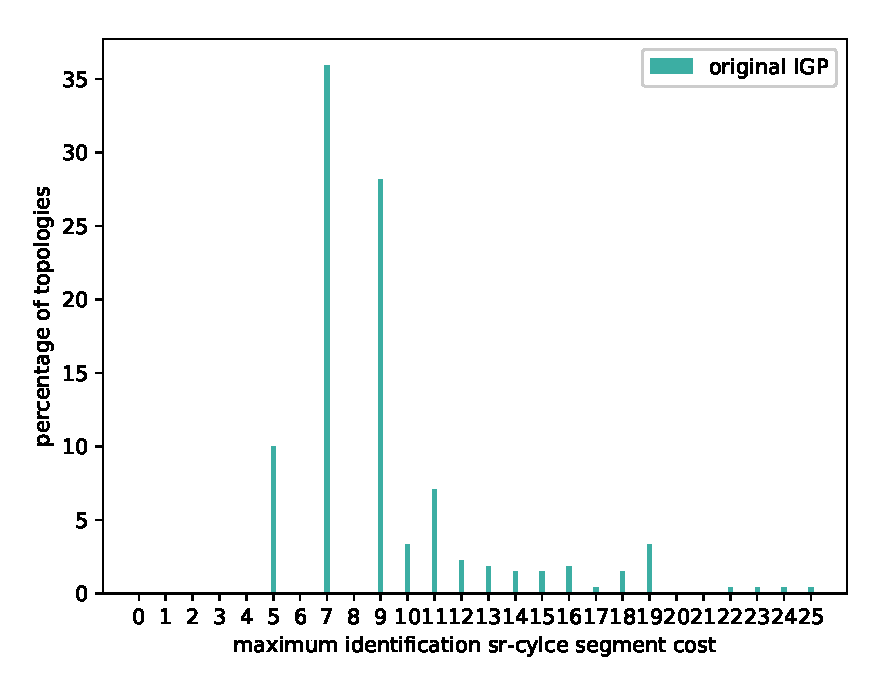
\includegraphics[width=.85\columnwidth]{./Network-lib/data/plot/minSegCover_identification_orig.eps}
\end{center}
\caption{Distribution of the maximum segment cost of the probing sr-cycles.}
\label{fig:min-seg-cost-segcost-orig}
\end{figure}


\begin{algorithm}[t]
\small
\caption{$\textsf{find-faulty-edge}\left( g, \sr{c} = \langle x_1, \ldots, x_l \rangle \right)$}
\begin{algorithmic}[1]
\STATE $c = (e_1, \ldots, e_n) \gets \seq(\sr{c})$
\STATE $L \gets 0, R \gets n$
\WHILE{$R - L \geq 2$}
  \STATE $i \gets \frac{L + R}{2}$
  \IF{$g.\textsf{isSymmetric}()$}
    \STATE $j \gets \min \ \left\{ j \in \{ 1, \ldots, l \} \mid e_i = x_j \vee \left(j < l \wedge e_i \in \sp(x^2_{j}, x^1_{j + 1})\right) \right\}$
    \IF{$e_i = x_j$}
      \STATE $\sr{c}_i \gets \langle x_1, \ldots, x_j, \rev(x_j), \ldots, \rev(x_1) \rangle$
    \ELSE
      \STATE $\sr{c}_i \gets \langle x_1, \ldots, x_{j - 1}, e^2_i, \rev(x_{j - 1}), \ldots, \rev(x_1) \rangle$
    \ENDIF
  \ELSE
    \STATE $\sr{c}_i \gets \textsf{min-segmentation}((e_1, \ldots, e_i, \rev(e_i), \ldots, \rev(e_1))$
  \ENDIF
  \STATE $\textit{status} \gets \textsf{send-probe}(\sr{c}_i)$
  \IF{$\textit{status} = \textit{received}$}
    \STATE $L \gets M$
  \ELSE
    \STATE $R \gets M$
  \ENDIF
\ENDWHILE
\IF{\textit{single-link failures}}
  \RETURN $e_L$
\ENDIF
\RETURN $\{ e_L, \rev(e_L) \}$
\end{algorithmic}
\label{algo:findedge}
\end{algorithm}

% 
% \subsection{Computing the cycle cover}
% 
% 
% \subsection{Min segment cost cycle cover}
% 
% \begin{lemma}
% \label{lemma:deterministic-concat2}
% Let $\sr{p} = \langle x_1 \ldots, x_l \rangle$ be a deterministic sr-path from $u_1$ to $u_2$ and 
% $\sr{q} = \langle y_1, \ldots, y_r \rangle$ be a sr-path from
% $v_1$ to $v_2$ such that $u_2 \neq v_1$ and $v_1 \in \nreach(u_2, 1)$. Then $\sr{p} \oplus \sr{q}$
% is a deterministic sr-path from $u_1$ to $v_2$ with 
% 
% \[ \cost(\sr{p} \oplus \sr{q}) =
%   \begin{cases}
%     \cost(\sr{p}) + \cost(\sr{q}) + 1 & \quad \text{if } y_1 \text{ is a node segment}\\
%     \cost(\sr{p}) + \cost(\sr{q})  & \quad \text{otherwise}
%   \end{cases}
% \]
% \end{lemma}
% 
% \begin{proof}
% The fact that $\sr{p} \oplus \sr{q}$ is deterministic is obvious since both $\sr{p}$ and $\sr{q}$ are deterministic and
% since $v_1 \in \nreach(u_2, 1)$ there is a unique shortest path connecting the last node of $\sr{p}$ to the first node of
% $\sr{q}$. Write $\sr{p} \langle x_1 \ldots, x_l \rangle$ and $\sr{q} = \langle y_1, \ldots, y_r \rangle$. If $y_i$ is a node
% segment, its cost is not included in $\sr{q}$ since it is the ingress node of that sr-path. However, it appears as a segment in 
% $\sr{p} \oplus \sr{q}$ since $u_2 \neq v_1$. Therefore in this case the segment cost in increased by $1$. Otherwise $y_i$ was already
% counted in $\cost(\sr{q})$ so the segment cost is just the sum of both costs. Note that the nature of $x_1$ does not matter as it remains
% the origin of the concatenation of the sr-paths.
% \end{proof}
% 
% \begin{lemma}
% \label{lemma:splitCost}
% Let $\sr{p} = \langle x_1, x_2, \ldots, x_l \rangle$. Then, for all $v \in V(G)$ and $i = 1, \ldots, l$ we have that
% $$
% \cost(\langle u, x_{i + 1}, \ldots, x_l \rangle) = \cost(\sr{p}) - \cost(\langle x_1, \ldots, x_i \rangle)
% $$
% \end{lemma}
% 
% \begin{proof}
% Since $u$ is a node segment, $\cost(\langle u, x_{i + 1}, \ldots, x_l \rangle) = \sum_{k = i + 1}^l \cost(x_k)$.
% On the other hand,
% \begin{align*}
% \cost(\sr{p}) - \cost(\langle x_1, \ldots, x_i \rangle) & = \sum_{k = 1}^l \cost(\sr{p}, x_i) - \sum_{k = 1}^i \cost(\sr{p}, x_i) \\
% & = \sum_{k = i + 1}^l \cost(\sr{p}, x_i) \\
% & = \cost(\langle u, x_{i + 1}, \ldots, x_l \rangle)
% \end{align*}
% \end{proof}
% 
% \begin{lemma}
% \label{lemma:splitCost2}
% Let $\sr{p} = \langle x_1, x_2, \ldots, x_l \rangle$, $i \in \{ 1, \ldots, l - 1 \}$, $k = \cost(\sr{p})$, $k_1 = \cost(\langle x_1, \ldots, x_i \rangle)$ 
% and $k_2 = \cost(\langle x_{i + 1}, \ldots, x_l \rangle)$. Then, 
% \[ k_2 =
%   \begin{cases}
%     k - k_1 - 1 & \quad \text{if } x_{i + 1} \text{ is a node segment}\\
%     k - k_1  & \quad \text{otherwise}
%   \end{cases}
% \]
% \end{lemma}
% 
% \begin{proof}
% We have that
% \begin{align*}
% k_2 & = \cost(\langle x_{i + 1}, \ldots, x_l \rangle) = \sum_{j = i + 1}^l \cost(x_j) \\
% \end{align*}
% If $x_{i + 1}$ is an adjacency segment then
% \end{proof}
% 
% 
% \begin{theorem}
% \label{thm:cyclecover}
% Let $G$ be a network, $s \in V(G)$ and $e \in E(G)$.
% There exists a deterministic sr-cycle $\sr{c}$ from $s$ to $s$ of segment cost at most $k$ covering $e = (u_1, u_2)$ if and only
% there exists $r \in \{0, \ldots, k\}$ such that one of these conditions holds
% \begin{enumerate}
%  \item $(u_1, u_2) \in \ereach(r, s)$ and $v \in \nreach(k - r, u_2)$
%  \item there exists $x \in \nreach(r, s)$ and $y \in \nreach(x, 1)$ such that $e \in \sp(x, y)$ and $s \in \nreach^n(k - r - 1, y)$
%  \item there exists $x \in \nreach(r, s)$ and $y \in \nreach(x, 1)$ such that $e \in \sp(x, y)$ and $s \in \nreach^e(k - r, y)$
% \end{enumerate}
% \end{theorem}
% 
% \begin{proof}
% $(\Rightarrow)$ Suppose that $c = \langle x_1, \ldots, x_l \rangle$ is a deterministic sr-cycle from $s$ to $s$ of segment cost at most $k$ covering $e$.
% Since $c$ covers $e$, there exists the smallest $i$ such that $\langle x_1, \ldots, x_i \rangle$
% covers edge $e$.
% 
% \emph{Case 1:} $x_i = e$: Write $r = \cost(\langle x_1, \ldots, x_i \rangle)$. Then, by Lemma \ref{lemma:splitCost},
% $\langle u_2, x_{i + 1}, \ldots, x_l \rangle$ is a sr-path of cost at most $k - r$ from $u_2$ to
% $s$. Hence $s \in \nreach(k - r, u_2)$.
% 
% \emph{Case 2:} $x_i \neq e$: Then, by choice of $i$, $e$ belongs to the unique shortest path betweeh $x^2_{i - 1}$ and $x^1_{i}$.
% Let $x = x^2_{i - 1}$, $y = x^1_i$ and $r = \cost(\langle x_1, \ldots, x_{i - 1} \rangle)$. 
% Then, since $c$ is deterministic, $x = x^2_{i - 1} \in \nreach(s, r)$ and $y = x^1_i \in \nreach(1, x)$.
% If $x_i$ is a node segment then $\langle x_{i + 1}, \ldots, x_l \rangle$ has cost $k - r - 1$ so $s \in \nreach^n(k - r - 1, y)$.
% Otherwise, $\langle x_{i + 1}, \ldots, x_l \rangle$ has cost $k - r$ so $s \in \nreach^e(k - r, y)$. Since $e \in \sp(x, y)$ we 
% see that either condition $2.$ or $3.$ from the above theorem is satisfied.
% 
% $(\Leftarrow)$ Suppose that there exists $r$ such that $(u_1, u_2) \in \ereach(v, r)$ and $v \in \nreach(u_2, k - r)$.
% There there exists a sr-path $\sr{p}$ from $v$ to $u_2$ covering $e$ of segment cost at most $r$ and 
% a sr-path $\sr{q}$ from $u_2$ to $v$ of segment cost at most $k - r$. By Lemma \ref{lemma:deterministic-concat},
% $\sr{c} = \sr{p} \oplus \sr{q}$ is a deterministic sr-cycle from $v$ to $v$ covering edge $e$ with $\cost(\sr{c}) \leq r + k - r = k$
% 
% Suppose now that there exists $x \in \nreach(v, r)$ and $y \in \nreach(x, 1)$ such that $e \in \sp(x, y)$ and $v \in \nreach(y, k - r)$.
% Then there exists a sr-path $\sr{p}$ from $v$ to $x$ with $\cost(\sr{p}) \leq r$ and a sr-path $\sr{q}$ from $y$ to $v$
% with $\cost(\sr{q}) \leq k - r$. Since $y \in \nreach(x, 1)$, by Lemma \ref{lemma:deterministic-concat2} \todo{this lemma does not exists, concatenation of
% paths not ending in the same node but with unique shoretest path between}, $\sr{c} = \sr{p} \oplus \sr{q}$ is a deterministic sr-cycle
% from $v$ to $v$ with $\cost(\sr{c}) \leq r + k - r = k$. Since $e \in \sp(x, y)$ this cycle covers $e$.
% \end{proof}


\section{Dual topology monitoring}
\label{section:complete-igp}

As we showed before, the minimum number of segments required to cover a topology can be quite high.
One idea to reduce it is to have a separate set of IGP weights. The ones already configured on the network used
to forward traffic and new ones that are used only for sending the monitoring probes.

One idea to compute those weights would be to first compute a minimum cycle cover of the network using
some standard existing algorithm \cite{FAN1992113} (note that here we are talking about cycles, not 
sr-cycles). Then we could compute a set of weights such that the maximum number of segments required to
segment any of those cycles is as small as possible. We did not solve this problem and therefore leave
it as an open problem (with a slightly more general formulation).

\begin{problem}{Optimal segmentation IGP}
Given a graph $G$ and a set $P$ of paths on $G$ compute a IGP weight function 
$\igp : E(G) \rightarrow \mathbb{N}$ such that if we compute a minimal segmentation
of every path $p \in P$ whose maximum segment cost amongst those sr-paths is minimal.
\end{problem}

We believe that solving this problem could be very useful in any setting where having a dual weight
topology is infeasible in practice. This would be yet another way to leverage existing graph theory to solve the 
problem and then translate those graph theoretic solutions into segment routing solutions with low
segment cost.

Another possibility, which we explore in this thesis, is to compute a set of $\igp$ weights such that 
there is a unique shortest path between any pair of nodes \emph{and} every edge belongs to a unique shortest
path. The intuition of why this will make segmentations less costly is that the conditions for needing to add
a new segment in the minimum segmentation algorithm is exactly the existence of multiple shortest paths or
an edge that does not belong to any shortest path.
Note that our two conditions cannot both coexist in a network with parallel links. With two links between
$u$ and $v$, we cannot have at the same time that both those links belong to some shortest path and a unique
shortest path between $u$ and $v$. We therefore relax the definition as follows.

\begin{definition}
Let $G$ be a graph. A set of IGP weights $\igp : E(G) \rightarrow \mathbb{N}$ is said to be
\emph{complete} if and only if for all $u, v \in V(G)$ at least one edge of $E(G, u, v)$ belong to a shortest path.
\end{definition}

\begin{definition}
Let $G$ be a graph. A set of IGP weights $\igp : E(G) \rightarrow \mathbb{N}$ is said to be
\emph{ECMP-free} if and only if for all $u, v \in V(G)$ there is a unique shortest path between $u$ and $v$.
\end{definition}

\subsection{Computing ECMP-free and complete IGP weights}

\begin{definition}
Let $G$ be a graph. A set of IGP weights $\igp : E(G) \rightarrow \mathbb{N}$ is said to be
\emph{total} if and only all simple paths on $G$ have a different weight.
\end{definition}

Computing a total weighting of a graph $G$ is trivial. We can simply set $\igp(e) = 2^{\idx(e)}$ for
all $e \in E(G)$. Since $\idx(e)$ assigns a unique index between $0$ and $|E(G)| - 1$ to the edges
of $G$, this IGP function will assign a different power of two to each edge of $G$. Therefore,
any two distinct simple paths must have a different IGP weight since those weights will
correspond to sums of distinct powers of $2$.

The following lemma shows, unsurprisingly, that one way to build ECMP-free weights is to compute
total weights.

\begin{lemma}
\label{lemma:totalToECMP}
Let $G$ be a graph. If $\igp : E(G) \rightarrow \mathbb{N}$ is total then it is ECMP-free.
\end{lemma}

\begin{proof}
Trivial from the definition. Any shortest path is simple and thus any two shortest paths must 
have a different IGP weight since $\igp$ is total.
\end{proof}

The following result shows that we can transform any total IGP weighting $\igp$ into a complete one by
adding a large enough constant. This constant can by any value above the maximum between the diameter of the
graph with respect to $\igp$ and the maximum weight of any edge. Being larger than the diameter ensures
that shortest paths remain unique and being larger than the maximum weight ensures that every edge belong to a shortest path. 
The diameter of a network is the greatest distance (in terms of number of edges)
between any pair of vertices.

\begin{lemma}
\label{lemma:totalToComplete}
Let $G$ be a network. Let 
$$
M \geq \max \left( diam(G, \igp), \displaystyle \max_{e \in E(G)} \igp(e) \right).
$$
Then, if $\igp : E(G) \rightarrow \mathbb{N}$ is total then 
$\igp^+ : E(G) \rightarrow \mathbb{N}$ defined by $\igp^+(e) = \igp(e) + M$ is complete.
\end{lemma}

\begin{proof}
Let $p_1 = (e_1, \ldots, e_n)$ and $p_2 = (f_1, \ldots, f_m)$ be two paths on $G$. 

We start by proving that $\igp^+(p_1) \neq \igp^+(p_2)$. By definition
$\igp^+(p_1) = \igp(p_1) + n \cdot M$ and $\igp^+(p_2) = \igp(p_2) + m \cdot M$. By hypothesis, 
$\igp(p_1) \neq \igp(p_2)$ Assume without loss of generality that $\igp(p_1) > \igp(p_2)$. If $n = m$ then
\begin{align*}
\igp^+(p_1) = \igp(p_1) + n \cdot M > \igp(p_2) + n \cdot M = \igp(p_2) + m \cdot M = \igp^+(p_2).
\end{align*}
By definition of $M$, we have $M \geq diam(G, \igp) \geq \igp(p_1), \igp(p_2) > 0$. Thus, if $n > m$ then,
\begin{align*}
\igp^+(p_1) & = \igp(p_1) + n \cdot M > n \cdot M \geq (m + 1) \cdot M \\
& = M + m \cdot M \geq \igp(p_2) + m \cdot M = \igp^+(p_2)
\end{align*}
Similarly, if $n < m$ then
\begin{align*}
\igp^+(p_2) & = \igp(p_2) + m \cdot M > m \cdot M \geq (n + 1) \cdot M \\
& = M + n \cdot M \geq \igp(p_1) + n \cdot M = \igp^+(p_1).
\end{align*}
Thus, in any case, $\igp^+(p_1) \neq \igp^+(p_2)$. We conclude that $\igp^+$ is total
and therefore also ECMP-free.

Let $u, v \in V(G)$. We now show that at least one edge $e \in E(G, u, v)$ belongs to a shortest path with respect to $\igp^+$.
Let $e \in E(G, u, v)$ be such that $\igp(e)$ is minimum. Since $\igp$ is total, this edge is unique. 
By Proposition \ref{prop:sp-properties}, $e$ belongs to a shortest path if and only if $e$ is a shortest path between
$u$ and $v$. Suppose that $e$ is not a shortest path for $\igp^+$. Then there exists a path $p = (e_1, \ldots, e_n)$ from $u$ to $v$ such that
$\igp^+(p) < \igp(e)$. Since $e$ is the unique edge between $u$ and $v$ of minimum cost, $n \geq 2$. By definition of $M$, we have $M \geq \igp(e)$ so 
\begin{align*}
\igp^+(p) = \igp(p) + n \cdot M \geq \igp(p) + 2 \cdot M > 2 \cdot M \geq 2 \cdot \igp(e) > \igp(e).
\end{align*}
This contradicts the fact that $e$ is not a shortest path for $\igp^+$. Therefore $\igp^+$ is complete.
\end{proof}

\begin{corollary}
Let $G$ be a graph and $\igp : E(G) \rightarrow \mathbb{N}$ defined such that
$$
\igp(e) = 2^{\idx(e)} + 2^{|E(G)|}.
$$
Then $\igp$ is ECMP-free and complete.
\end{corollary}

\begin{proof}
We have already observed that $e \mapsto 2^{\idx(e)}$ is total and thus ECMP-free by Lemma \ref{lemma:totalToECMP}. Completeness then follows from
Lemma \ref{lemma:totalToComplete} by observing that 
$$
2^{|E(G)|} = \left( \sum_{e \in E(G)} 2^{\idx(e)} \right) + 1 > \max \left( diam(G, \igp), \displaystyle \max_{e \in E(G)} \igp(e) \right).
$$
\end{proof}

The problem with these IGP weights is that they are exponential with respect to the number of edges in the graph.
In practice IGP weights are represented with a $16$-bit integer and thus is maximum value is $2^{16} - 1 = 65535$.
This makes them useless in practice since they can only be implemented on a network with at most $15$ edges.

This motivates the following problem.

\begin{problem}{Minimum weight complete weighting}
\label{prob:minComplete}
\textbf{Input:} A network $G$.

\textbf{Output:} A complete and ECMP-free weighting $\igp : E(G) \rightarrow \mathbb{N}$ such that
$\displaystyle \max_{e \in E(G)} \igp(e)$ is minimum.
\end{problem}

Any approach for solving Problem \ref{prob:minComplete} that is based on Lemma \ref{lemma:totalToComplete} is domed to fail.
To see why this is true consider $\mathcal{K}_n$, the complete graph on $n$ nodes. It is not hard to see that $\mathcal{K}_n$ 
contains an exponential number of simple paths. 

%Any simple path on $\mathcal{K}_n$ corresponds to a sequence of nodes
%of length at most $n - 1$ without repetitions. Therefore, the number of such paths is
%$$
%P = \frac{1}{2} \sum_{l = 2}^n \frac{n!}{(n - l)!} \approx \frac{en!}{2}.
%$$

Any permutation of $n$ elements corresponds to a simple path on $\mathcal{K}_n$ 
of length $n - 1$ and there are $n!$ permutations of $n$ elements. Since a total weight must assign a different weight to
\emph{every} simple path, this shows that a total weight on the complete graph $\mathcal{K}_n$ will be such that at least
one simple path of length $n - 1$ has a weight of at least $n!$. Therefore this path must contain one edge of weight
$\frac{n!}{n - 1}$ since otherwise the total weight of the path would be lower than $n!$.

This shows that total weightings require exponential weights on any graph with an exponential number of paths. Most graphs
have an exponential number of simple paths with respect to its size. Hence, using Lemma \ref{lemma:totalToComplete} is bound
to provide weights that are very high. In contrast, it is not hard to see that $e \mapsto 1$ is an ECMP-free and complete weighting of
$\mathcal{K}_n$. This shows that such exponential bounds do not apply for the weight that we are looking for, only for total ones.

If we only care about the practical applicability of the weights, we can relax Problem \ref{prob:minComplete} into the following one.

\begin{problem}{Implementable complete weighting}
\label{prob:implemComplete}
\textbf{Input:} A network $G$.

\textbf{Output:} A complete and ECMP-free weighting $\igp : E(G) \rightarrow \mathbb{N}$ such that
$\displaystyle \max_{e \in E(G)} \igp(e) \leq 2^{16} - 1$.
\end{problem}

\subsection{Prime-based complete IGP}

We propose a partial solution to Problem \ref{prob:implemComplete}. Our solution is able to find a solution for $97.7\%$ of the instances in our dataset.
Let $m = |E(G)|$ be the number of edges in the graph and $\mathbb{P}_m = \{ \pi_0, \ldots, \pi_{m - 1} \}$ a set of $m$ prime numbers such that
$\pi_i \leq \pi_{i + 1}$. It is well known that two sets of distinct prime numbers
have a different product. Our idea is based on the fact that $\log(x \cdot y) = \log(x) \cdot \log(y)$. If we could set any real valued IGP weights,
one solution would be to use $e \mapsto \log(\pi_{\idx(e)})$ because the unicity of products between prime numbers would translate into unique sums
and thus unique path weights. To simplify the notations, we write $\pi_e$ instead of $\pi_{\idx(e)}$.
In this way, by what we observe above, two distinct paths would necessarily have distinct IGP costs.

Since we need integers we will use truncated logarithms instead. These logarithms are defined as
$$
\lnt{s}(x) = \lfloor 10^s \cdot \ln(x) \rfloor.
$$
For instance, $\lnt{4}(5) = \lfloor 10^4 \cdot 1.60943 \rfloor = 16094$. The idea is, starting from $s = 1$, to grow $s$ 
until the IGP weights defined by $e \mapsto \lnt{s}(\pi_e)$ are ECMP-free. A priori, nothing guarantees that doing so will 
eventually achieve it but we will prove shortly that it does. Since we also want the IGP weights to also be complete, we use
a slight different set of IGP weights $\igp^s : E(G) \rightarrow \mathbb{N}$ defined as $\igp^s(e) = \lnt{s}(\pi_e) + \lnt{s}(\pi_m)$.
The intuition behind the addition of the largest $\lnt{s}(\pi_m)$ term for achieving completeness is similar to the addition of the constant $M$
from Lemma \ref{lemma:totalToComplete}. We now prove that by growing $s$, $\igp^s$ eventually becomes ECMP-free and complete.

  
\begin{proposition}
\label{prop:converge}
Let $A$ and $B$ be two distinct subsets of $\mathcal{P}_m$, $P = \prod_{x \in \mathcal{P}_x} x$ and $q \in \mathcal{P}_m$. If $s > \log_{10} \left( 2 m \cdot q^m P \right)$, 
then 
$$
\sum_{x \in A} \left( \overline{\ln}^s(x) + \overline{\ln}^s(q) \right) \neq \sum_{x \in B} \left( \overline{\ln}^s(x) + \overline{\ln}^s(q) \right).
$$
\end{proposition}

\begin{proof}
Given any $s$ and $X \subseteq \mathcal{P}_m$, we have
\begin{equation}
\small
\label{eq:lg}
10^s \cdot \ln \left( \prod_{x \in X} x \right) \geq \sum_{x \in X} \overline{\ln}^s(x) \geq 10^s \cdot \ln \left( \prod_{x \in X} x \right) - |X|
\end{equation}

Let $q \in \mathcal{P}_m$. Write $a = \prod_{x \in A} x$ and $b = \prod_{x \in B} x$. Assume without loss of generality that $q^{|A|} a > q^{|B|} b$ (they are not equal because they contain distinct prime numbers). 
Then by (\ref{eq:lg})
\begin{align*}
\tiny
\sum_{x \in A} \overline{\ln}^s(x) +  \overline{\ln}^s(q) & \geq \sum_{x \in A} 10^s \ln(x q) - 2 \geq \\
& 10^s \ln(q^{|A|} a) - 2 |A|
\end{align*}
and $\sum_{x \in B} \overline{\ln}^s(x) + \overline{\ln}^s(q) \leq 10^s \ln (q^{|B|} b)$. Therefore
\begin{align*}
\tiny
\sum_{x \in A} \overline{\ln}^s(x) +  \overline{\ln}^s(q) - \sum_{x \in B} \overline{\ln}^s(x) + \overline{\ln}^s(q) & \geq \\
10^s \ln(q^{|A|} a) - 2 |A| - 10^s \ln (q^{|B|} b) & \geq \\
10^s  \ln \left(q^{|A|} a \slash q^{|B|} b \right) - 2 |A| \geq & \\
10^s  \ln \left(q^{|A|} a \slash (q^{|A|} a - 1) \right) - 2 |A| \geq & \\
10^s \slash (q^{|A|} a) - 2|A| \geq 10^s \slash (q^m P) - 2m
\end{align*}
Which is positive as long as $s > \log_{10} \left( 2 m \cdot q^m P \right)$.
\end{proof}

\begin{corollary}
If $s > \log_{10} \left( 2 m \cdot q^m P \right)$ then $\igp^s$ is ECMP-free.
\end{corollary}

\begin{proof}
Let $p_1, p_2$ be two paths on $G$ and $q = \pi_m$. By Proposition \ref{prop:converge}, 
$$
\igp^s(p_1) = \sum_{e \in E(p_1)} \left( \overline{\ln}^s(e) + \overline{\ln}^s(\pi_m) \right) \neq \sum_{e \in E(p_2)} \left( \overline{\ln}^s(e) + \overline{\ln}^s(\pi_m) \right) = \igp^s(p_2).
$$
Therefore $\igp^s$ is total and thus, by Lemma \ref{lemma:totalToComplete}, this means that 
it will also be ECMP-free.
\end{proof}

\begin{proposition}
The weights $\igp^s$ are complete for any $s \geq 1$.
\end{proposition}

\begin{proof}
Let $u, v \in V(G)$. Assume that the shortest path $p$ from $u$ to $v$ is not a single edge.
Let $e$ be any edge between $u$ and $v$. Then,
\begin{align*}
\tiny
w(p) & = |E(p)| \cdot \overline{\ln}^s(\pi_m) + \sum_{e \in E(P)} \overline{\ln}^s(\pi_e) > |E(p)| \cdot \overline{\ln}^s(\pi_m) \geq \\
& 2 \cdot \overline{\ln}^s(\pi_m) \geq \overline{\ln}^s(\pi_e) + \overline{\ln}^s(\pi_m) = w(e)
\end{align*}
Therefore $p$ cannot be a shortest path proving that $\igp^s$ is complete.
\end{proof}

These results provide a theoretical guarantee that the above mentioned process will eventually converge towards 
ECMP-free and complete weights. However, even for small graphs the value of $\log_{10} \left( 2 m \cdot q^m P \right)$ is
large and thus, if $s > \log_{10} \left( 2 m \cdot q^m P \right)$, then $10^s$ will be really huge. But this a theoretical bound on how long we need to wait to reach a \emph{total} function.
But we do not care about totality, we only want ECMP-freeness (completeness is true for any $s$). Therefore, our algorithm
will iterate over $s$ and, at each step, check whether ECMP-freeness holds with the hope that this will occur a long time before
totality occurs. Our experiments show that this is indeed the case. Figure \ref{fig:primeIGP_s} shows the distribution of the
value of $s$ over all topologies from out dataset. We can see that this value is indeed much smaller than the theoretical bound.

\begin{figure}
\begin{center}
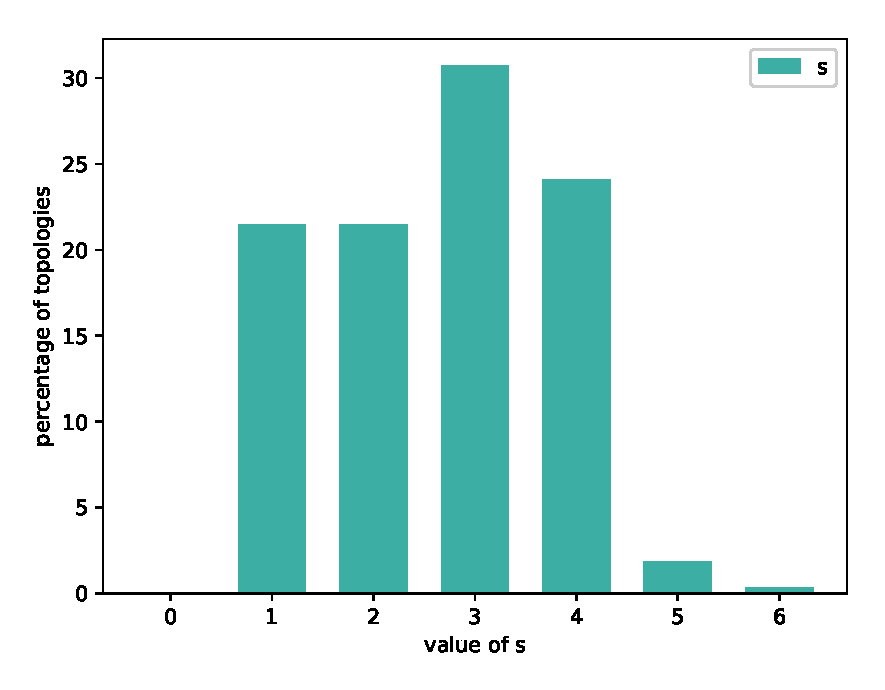
\includegraphics[width=.85\columnwidth]{./Network-lib/data/plot/primeIGP_s.eps}
\end{center}
\caption{Distribution, over all topologies, of the exponent $s$ required for $\igp^s$ to be ECMP-free and complete.}
\label{fig:primeIGP_s}
\end{figure}

We analyzed the percentage of topologies for which this process results in weights that go above the maximum configurable value $2^{16} - 1$.
It turns out that for this happens only for $2.3\%$ of the topologies as show in the CDF in Figure \ref{fig:primeIGP}. The threshold value
is shown with a dotted line.

\begin{figure}
\begin{center}
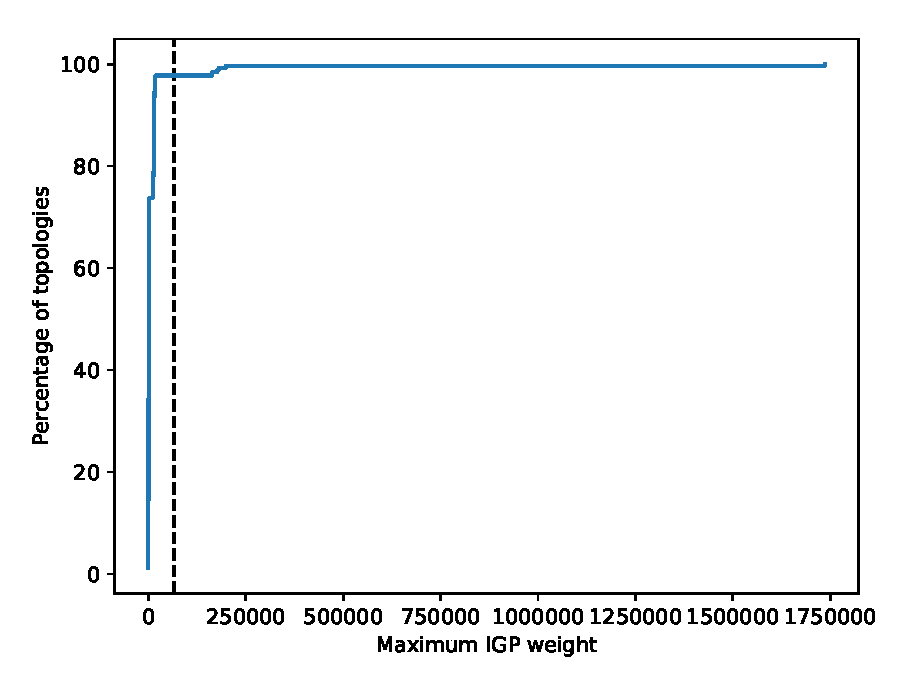
\includegraphics[width=.85\columnwidth]{./Network-lib/data/plot/primeIGP.eps}
\end{center}
\caption{CDF of maximum weight obtained over all topologies.}
\label{fig:primeIGP}
\end{figure}

Algorithm \ref{algo:primeIGP} provides a pseudo-code implementation of this algorithm described above.
The first step of the algorithm is to compute a set of $m = |E(G)|$ prime numbers. We can find these by iterating over the integers $2, 3, 5, 7, 9, \ldots$
and using any primality test algorithm to check which ones are prime numbers. The Prime number theorem \cite{Cormen:2009:IAT:1614191} %page 888 theorem 31.37
tells us that the $m$-th prime number is close to $m \cdot \ln(m)$ so we find them in a small number of steps.
This is not the most efficient way to achieve this but since $m$ is relatively small it is fast enough for our purposes.

\begin{algorithm}[t]
\small
\caption{$\textsf{primeIGP}\left( G \right)$}
\begin{algorithmic}[1]
%\algrule
\cmtline{compute the first $|E(G)|$ primes}
\STATE $m \gets |E(G)|$
\STATE $\mathcal{P} \gets \{ 2 \}$
\STATE $p \gets 3$
\WHILE{$|\mathcal{P}| < m$}
  \IF{$\textsf{isPrime}(p)$}
    \STATE $\mathcal{P} \gets \mathcal{P} \cup \{p\}$
  \ENDIF
  \STATE $p \gets p + 2$
\ENDWHILE
\cmtline{initialize weights}
\STATE $f \gets 1$
\FOR{$e \in E(G)$}
  \STATE $w(e) \gets \lfloor f \cdot \log(p_e) \rfloor + \lfloor f \cdot \log(p_m) \rfloor$
\ENDFOR
\cmtline{iterate until weights converge}
\WHILE{\textbf{not} $\textsf{ECMP-free}(w)$ \textbf{or not} $\textsf{complete}(w)$}
  \STATE $f \gets 10 \cdot f$
  \FOR{$e \in E(G)$}
    \STATE $w(e) \gets \lfloor f \cdot \log(p_e) \rfloor + \lfloor f \cdot \log(p_m) \rfloor$
  \ENDFOR
\ENDWHILE
\RETURN $w$
\end{algorithmic}
\label{algo:primeIGP}
\end{algorithm}

\subsection{Randomized complete IGP}

In practice, there seems to be a much simpler solution for generating relatively small ECMP-free and complete IGP weights.
We performed some experiments that showed that random weighs tend to be ECMP-free as long as the maximum value is not too small.
Therefore, a solution for generating ECMP-free weights that are also complete is to randomly generate weights for each edge 
and then adding the maximum generated weight to each edge to guarantee completeness. Algorithms \ref{algo:randomIGP} and \ref{algo:randomw}
formalize this process. Note that without the step of adding the maximum weight, our experiments showed that the algorithm
has a low probability of success. This is normal because otherwise there is no control over the weight of a single edge 
and so it can easily happen that it is assigned a high value making it impossible for it to belong to a shortest path.

\begin{algorithm}[t]
\small
\caption{$\textsf{randomIGP}\left( G, M \right)$}
\begin{algorithmic}[1]
%\algrule
\STATE $w \gets \textsf{random-w}(G, M)$
\WHILE{\textbf{not} $\textsf{ECMP-free}(w)$ \textbf{or not} $\textsf{complete}(w)$}
  \STATE $w \gets \textsf{random-w}(G, M)$ 
\ENDWHILE
\RETURN $w$
\end{algorithmic}
\label{algo:randomIGP}
\end{algorithm}

\begin{algorithm}[t]
\small
\caption{$\textsf{random-w}\left( G, M \right)$}
\begin{algorithmic}[1]
%\algrule
\FOR{$e \in E(G)$}
  \STATE $w(e) \gets \textsf{random}(1, \ldots, M)$
\ENDFOR
\FOR{$e \in E(G)$}
  \STATE $w'(e) \gets w(e) + \max_{e \in E(G)} w(e)$
\ENDFOR
\RETURN $w'$
\end{algorithmic}
\label{algo:randomw}
\end{algorithm}

In practice we tried it over all topologies with $M = 100$ for each of them we found a solution on average in at most $2$ iterations (over $100$ runs).
For this reason, in practice we strongly recommend using this simple algorithm. However we were unable to prove any bound on the probability of success
of this algorithm. Hence we cannot say whether it will work well beyond our dataset. We leave the following problem as another interesting open problem.

\begin{lemma}
For any network $G$ and $M \in \mathbb{N}$ the weight function produced by Algorithm \ref{algo:randomw} is complete. 
\end{lemma}

\begin{proof}
Let $w$ be the random weights produced by the algorithm after the first loop and $w'$ the final weights. Let $M = \max_{e \in E(G)} w(e)$. 
Let $u, v \in V(G)$ and $p$ be a path from $u$ to $v$ with at least two edges.
Then
$$
w'(p) = w(p) + |E(p)| \cdot M > 2 \cdot M \geq w(e) + M = w'(e)
$$
for any edge $e \in E(G)$. Therefore the shortest path between $u$ and $v$ must be a single edge $e \in E(G, u, v)$.
\end{proof}

\begin{problem}{Randomized weighting}
\label{prob:randomIGP}
\textbf{Input:} A network $G$ and a integer constant $M \in \mathbb{N}$. 

\textbf{Output:} The probability that $\textsf{random-w}\left( G, M \right)$ outputs an ECMP-free IGP weight function.
\end{problem}

\subsection{Cycle covers with ECMP-free and complete IGP}

In this section we evaluate the benefits of using ECMP-free and complete IGP weights.
We start by evaluating the minimum number of segments required in a minimum segment cost
sr-cycle cover. Recall that Algorithm \ref{algo:min-seg-cover2} computes a sr-cycle cover such
that the maximum number of segments in any sr-cycle is as small as possible. In Figure 
\ref{fig:min-seg-cover-segcost} we already evaluated the segment cost of the solutions obtained 
by this algorithm over the original IGP weights. Figure \ref{fig:min-seg-cost-segcost-new} shows
the distribution of the segment costs with and without special IGP weights. We observe that ECMP-free
and complete weights obtain the desired effect of greatly reducing the segment cost of minimum
cost sr-cycle covers. For $100\%$ of the topologies we need sr-cycles with segment cost at most $4$ whereas before
about $55\%$ of the topologies required sr-cycles with segment cost $5$ or more.

\begin{figure}
\begin{center}
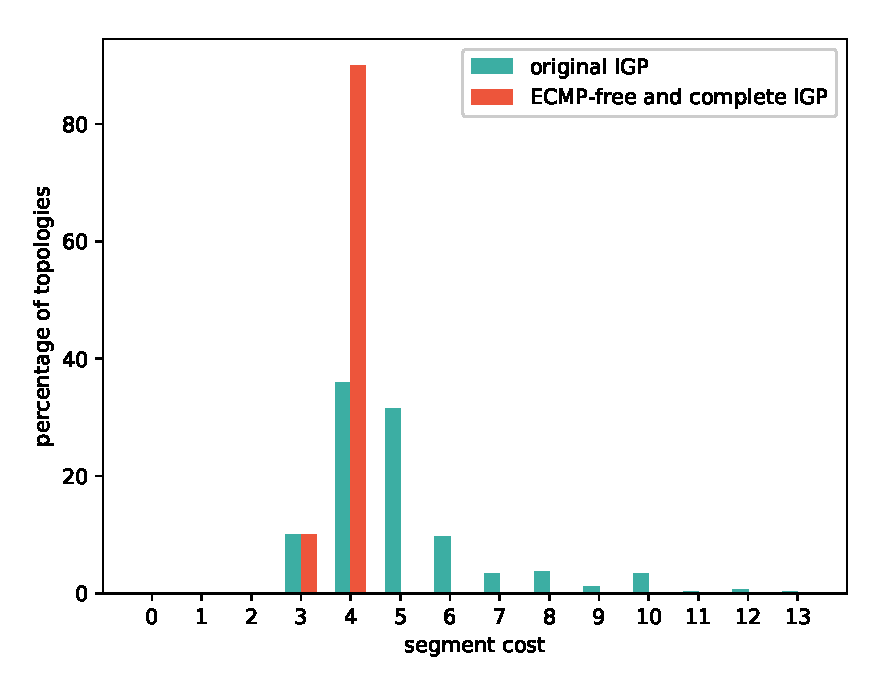
\includegraphics[width=.85\columnwidth]{./Network-lib/data/plot/minSegCover_segcost_complete.eps}
\end{center}
\caption{Distribution of the maximum segment cost of the probing sr-cycles with and without ECMP-free and complete weights.}
\label{fig:min-seg-cost-segcost-new}
\end{figure}

Next we analyze the benefits of using special IGP weights with respect to the segment cost of the 
identification sr-cycles. Recall that our network monitoring solution uses probing sr-cycles to periodically
check whether every link is still up and one identification sr-cycles to pinpoint a failure when
a monitoring probe fails to return to the vantage point. Figure \ref{fig:min-seg-cost-segcost-new}
shows how much do we gain in terms of segment cost by having ECMP-free and complete IGP weights. We can see that
using these weights makes it possible to implement such a monitoring scheme on a lot more networks since the maximum
number of segments required becomes $9$ rather than the original high value of $19$.

\begin{figure}
\begin{center}
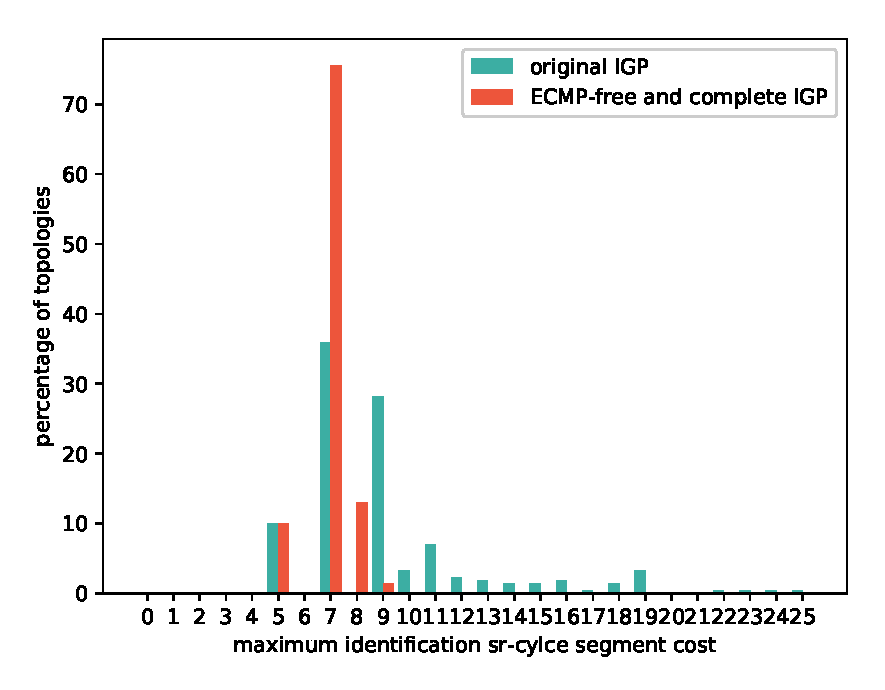
\includegraphics[width=.85\columnwidth]{./Network-lib/data/plot/minSegCover_identification.eps}
\end{center}
\caption{Distribution of the maximum segment cost of the identification sr-cycles with and without ECMP-free and complete weights.}
\label{fig:min-seg-cost-segcost-new}
\end{figure}


\section*{Conclusion}

In this chapter we proposed a solution for identifying single-link failures in a network.
We showed that even if multiple failures occur, our algorithm can still identify a pair of 
edges $e$, $\rev(e)$ such that one of them is faulty with certainty.

Our experiments show that our algorithm runs in a reasonable amount of time considering that
these cycles need to be installed only once in the network. 

Our solution works on the original topology and prides the theoretical minimum number of segments
required to implement any cycle cover using segment routing. This was achieved by using our reachability
theory developed in Chapter \ref{chapter:sr}. We also showed that if this segment cost
is too high, we can reduce it by working with a dual topology maxing the whole network monitoring 
process cost at most $9$ segments in the worst case, over all topologies from out dataset.

This was a second example where column generation provides good results when applied to solve an
segment routing optimization problem.

\chapter{Disjoint paths with SR}
\label{chapter:disjoint}

\section*{Introduction}

For an Internet Service Provider (ISP), providing disjoint paths to its
customers might be one of those advanced connectivity services that generate
more revenues. This is what emerged from our discussion with a national ISP that
we call ``reference ISP''. When we met them, this ISP's operators themselves
steered the discussion towards possibilities to provide disjoint paths between
sites to which a customer is connected. They were motivated by requests from
banks and financial customers.

We have quickly realized that the disjoint-path connectivity service has a much
bigger market than our reference ISP. An illustration is provided by the
NANOG email discussion about a major outage of the Bell network on August
4th, 2017~\cite{refnanog}. The email thread started with Bell's customers
complaining that both Internet and mobile connectivity were completely absent in
East Canada, affecting banking, ATM, land lines and even 911 services. When a
single fibre cut was indicated as the cause of the outage, someone expressed
doubts that ISPs really provide geographically diverse circuits, irrespectively
of what they promise and sell. The following emails discussed the impossibility
to work around this limitation by relying on two providers, as their networks
may share the same physical infrastructure (fibres, conduit, etc.), without the
ISPs even knowing it -- as they do not share information between each other.

The discussion we had with the reference ISP's operators was indeed focused on
\textit{providing disjoint paths within a single ISP}, their own. A possible
solution~\cite{art:2014} to achieve this goal is to deploy two parallel
networks, say a red and a blue copy of the same topology, and configure the
intra-domain routing protocol (IGP) so that any packet is forwarded in only one of
the two networks -- i.e., packets that enter the red copy are only forwarded in
the red copy.
The few links between the two networks are only used if one of the two copies is
partitioned. This architecture provides disjoint paths by design, but it is very
expensive since the entire network is doubled.
The reference ISP's operators were therefore reluctant to deploy it.
%The operators discarded solutions
%based on adding physical redundancy, like the 1+1 protection scheme in optical
%networks~\cite{}, because of the additional costs. 
Of course, they were also aware that MPLS tunnels can be created over
arbitrary paths with RSVP-TE~\cite{rfc3209}, including disjoint ones, on an
existing infrastructure.
However, they were in the process of moving away from MPLS, in order to avoid
its operational limitations~\cite{mpls-opissues-ripe64}, its sub-optimal usage
of resources~\cite{mpls-latency-imc11} and its scalability challenges with
respect to the routers' state~\cite{rfc5439,defo-sig15}.

%including synchronization with the
%underlying IGP and control-plane overhead~\cite{}, scalability~\cite{} and
%latency inflation~\cite{mpls-latency-imc11}.

Looking at other ISPs, our operators were instead considering Segment Routing
(SR). Motivated by this, we dedicate this chapter to the study of the problem of computing and implementing disjoint paths over a network
with segment routing. We also provide a solution for leveraging some properties of sr-paths to
show how we can provide disjoint paths that are robust to link failures.


\section{Disjoint paths and network flows}
\label{section:dp}

The problem of computing disjoint paths in a graph is one of those ubiquitous problem that has driven
a lot of research over the years. Numerous algorithms exist for solving it, most of them being some variant
of the more general maximum flow problem \cite{suurballe1984quick, Ahuja}.

The maximum flow problem is the problem of finding the maximum amount of information that can
be sent between two given nodes in a network. It is closely related to the multi-commodity flow
problem that we studied in Chapter \ref{chapter:te}. Instead of being given a set of demands, we are given
a source $s \in V(G)$ and a destination $t \in V(G)$ and we are asked what is the maximum amount of traffic that can be routed 
between those two nodes without exceeding the capacity of any edge. Another way to see it is to 
imagine that we have an infinite amount of unit demands between $s$ and $t$ and we are asked what is the maximum
number of such demands that can simultaneously be routed of the network without exceeding any link capacity.

The maximum flow problem admits an IP formulation that is very similar to the formulation that we gave for the MCF. If we let $x_e$
define the amount of demands routed over edge $e$ it can be shown that the following LP models the problem \cite{Ahuja}.

\begin{center}
\begin{tabular}{crcllr}
\multicolumn{5}{l}{$\maxflow(G, s, t)$} \\[0.5cm] 
$\displaystyle \mathbf{max}$ & $\displaystyle \sum_{e \in \oute(s)} x_e$ & & & & \\[0.5cm]
$\textbf{s.t.}$ & $\displaystyle \sum_{e \in \delta^-(v)} x_{e} - \sum_{e \in \delta^+(v)} x_{e}$ & $=$    & $ 0$ & $\forall v \in V(G) \setminus \{ s, t \}$  &  \\[0.5cm]
                & $x_{e}$ & $\leq$ & $\bnd(e)$ & $\forall e \in E(G)$ & \\[0.5cm]
                & $x_{e}$ & $\in$ & $\mathbb{N}$
\end{tabular}
\end{center}

It is possible to show that the linear programming relaxation of this problem obtained by replacing $x_e \in \mathbb{N}$ by $x_e \geq 0$ 
is equivalent as long as the capacities are integral \cite{Ahuja}. This makes the maximum flow problem one of those rare cases where the integrality constraints no not increase the difficulty
of the problem. Numerous polynomial time algorithms have been developed for solving the maximum flow problem \cite{Edmonds:1972:TIA:321694.321699, dinitz, Goldberg:1988:NAM:48014.61051, Ahuja}.
If we set \emph{unit capacities} on the edges and think about the maximum flow problem as one answering the question of what is the maximum amount of unit demands that we can
route from $s$ to $t$, we see that we actually end up with the \emph{maximum number of disjoint path between $s$ and $t$}. This is the case
since each of the routed demands must follow a path that shares no edges with any of the other demand paths or otherwise some edge would carry at least two units
of traffic, thus exceeding its capacity.

In other words, this means that we can model the problem of computing the maximum number of edge-disjoint paths between $s$ and $t$ by replacing $\bnd(e)$
by $1$ in the $\maxflow$ model. By doing so, we obtain the following model which can also be solved efficiently.

\begin{center}
\begin{tabular}{crcllr}
\multicolumn{5}{l}{$\maxedp(G, s, t)$} \\[0.5cm] 
$\displaystyle \mathbf{max}$ & $\displaystyle \sum_{e \in \oute(s)} x_e$ & & & & \\[0.5cm]
$\textbf{s.t.}$ & $\displaystyle \sum_{e \in \delta^-(v)} x_{e} - \sum_{e \in \delta^+(v)} x_{e}$ & $=$    & $ 0$ & $\forall v \in V(G) \setminus \{ s, t \}$  &  \\[0.5cm]
                & $x_{e}$ & $\leq$ & $1$ & $\forall e \in E(G)$ & \\[0.5cm]
                & $x_{e}$ & $\in$ & $\mathbb{N}$
\end{tabular}
\end{center}

This model focuses solely one providing a maximum amount of paths. It does not care about the quality of those paths, for instance, in terms of latency. It turns out that if we wish to
minimize total latency of the path set we can still do it in polynomial time. This problem is known, in general, as the minimum cost maximum flow problem \cite{Ahuja}.
We can easily adapt the above model to obtain a set of $n$ disjoint paths (if they exist) whose total latency is as small as possible by
requiring the total flow out of $s$ to be $n$ and minimizing the sum of the latencies of the edges with a non-zero flow as shown in the following model.

\begin{center}
\begin{tabular}{crcllr}
\multicolumn{5}{l}{$\minlatedp(G, s, t)$} \\[0.5cm] 
$\displaystyle \mathbf{min}$ & $\displaystyle \sum_{e \in E(G)} \lat(e) \cdot x_e$ & & & & \\[0.5cm]
$\textbf{s.t.}$ & $\displaystyle \sum_{e \in \delta^-(v)} x_{e} - \sum_{e \in \delta^+(v)} x_{e}$ & $=$    & $ 0$ & $\forall v \in V(G) \setminus \{ s, t \}$  &  \\[0.5cm]
                & $\displaystyle \sum_{e \in \oute(s)} x_e$ & $=$ & $n$ & \\[0.5cm]
                & $x_{e}$ & $\leq$ & $1$ & $\forall e \in E(G)$ & \\[0.5cm]
                & $x_{e}$ & $\in$ & $\mathbb{N}$
\end{tabular}
\end{center}

If we want $n$ to be as large as possible we can simply first compute the optimal solution of $\maxedp(G, s, t)$ and set $n$ to that value.
Surprisingly, this problem can also be solved in polynomial time \cite{Ahuja}. Unfortunately, slight variations of this problem that are of interest for computer
networks quickly become \NPhard. For instance, if we want to minimize the maximum latency over all the paths rather than the latency sum, the problem is 
\NPhard~even if $n = 2$ \cite{minmax-disjoint-90, Li1990}. Another change that, perhaps surprisingly, makes the problem \NPhard~is to have two origins $s_1, s_2$ and two destinations
$t_1, t_2$ and ask for a pair of disjoint paths, one from $s_1$ to $t_1$ and another from $s_2$ to $t_2$ \cite{VYGEN199583}. One might naively think that we could get away by adding a fake node 
$s$ linked to both $s_1, s_2$ and link $t_1, t_2$ to some other fake $t$ and then compute the maximum flow from $s$ to $t$. Unfortunately, nothing in the model
forces the flow originating from $s_1$ to go to $t_1$ instead of $t_2$ (and vice-versa). In order to force some origin to destination assignment, we cannot rely on a
maximum flow model but rather on a multi-commodity flow model which, as we have already seen, is harder to solve. 


\section{Disjoint sr-paths}
\label{section:dpsr}

In the previous section we talked about the general problem of finding sets of disjoint paths over a network.
However, the paths found by these algorithms can be arbitrary and thus hard to implement with segment 
routing as we will show shortly.

In this section we redefine the problem in terms of segment routing and adapt the MIP models from
the previous section accordingly. We start by defining what disjoint sr-path are and the problem of finding
a maximum cardinality set of sr-paths.

\begin{definition}
Let $G$ be a network and $\sr{p}, \sr{q}$ be two sr-paths on $G$. We say that $\sr{p}$ and $\sr{q}$ are \emph{disjoint} if
$E(\sr{p}) \cap E(\sr{q}) = \emptyset$. 
\end{definition}

\begin{problem}{Maximum edge-disjoint sr-paths problem}
\label{prob:max-sr-edp}
\textbf{Input:} A network $G$, two nodes $s, t \in V(G)$ and $k \in \mathbb{N}$.

\textbf{Output:} A set of sr-paths $\{ \sr{p}_1, \ldots, \sr{p}_n \} \subseteq \Pk(s, t)$ such that for each $i \neq j$, $\sr{p}_i$ and $\sr{p}_j$
are disjoint and $n$ is maximum.
\end{problem}

Recall that in case of ECMP between two consecutive segments of $\sr{p}$, the set $E(\sr{p})$ contains the edges belonging to \emph{all} 
those ECMP paths. In other words, we are requiring all those shortest paths corresponding to $\sr{p}$ and $\sr{q}$ to be edge-disjoint.
This is necessary because we can never be sure where exactly the traffic will flow when using a sr-path. In this way, we ensure that no matter how traffic is routed
over ECMPs, no edge will carry packets from two distinct sr-paths $\sr{p}_i$ and $\sr{p}_j$. Figure \ref{fig:non-disjoint} illustrates this with source node $\node{a}$
and destination node $\node{h}$. The two sr-paths displayed
on it are not disjoint because there might both use edge $(\node{e}, \node{h})$ in the event of the green one using path 
$(\edge{a}{c}, \edge{c}{d}, \edge{d}{e}, \edge{e}{h})$ and the blue one using $(\edge{a}{b}, \edge{b}{e}, \edge{e}{h})$.
This can be prevented by, for instance, forcing the blue path to pass thought node $\node{f}$ as shown in Figure \ref{fig:disjoint}.

\begin{figure}
\begin{center}
\begin{tikzpicture}
\def\x{0}
\def\y{0}

\node[scale=0.15] (a) at (0.5 + \x,  0.5 + \y) {\router{a}{router}};
\node[scale=0.15] (b) at (0.5 + \x, -1.0 + \y) {\router{b}{router}};
\node[scale=0.15] (c) at (2.5 + \x,  0.0 + \y) {\router{c}{router}};
\node[scale=0.15] (d) at (4.5 + \x,  0.0 + \y) {\router{d}{router}};
\node[scale=0.15] (e) at (4.0 + \x, -2.0 + \y) {\router{e}{router}};
\node[scale=0.15] (g) at (6.0 + \x,  0.5 + \y) {\router{g}{router}};
\node[scale=0.15] (i) at (8.0 + \x,  0.0 + \y) {\router{i}{router}};
\node[scale=0.15] (h) at (7.0 + \x, -1.5 + \y) {\router{h}{router}};
\node[scale=0.15] (f) at (4.0 + \x, -3.5 + \y) {\router{f}{router}};
\node[scale=0.15] (j) at (8.0 + \x, -2.5 + \y) {\router{j}{router}};
\draw[line width=2] (a) edge[above, sloped] node[black] {} (b);
\draw[line width=2]  (a) edge[above, sloped] node[black] {} (c);

\draw[line width=2] (b) edge[above, sloped] node[black] {} (c);
\draw[line width=2] (b) edge[above, sloped] node[black] {} (e);
\draw[line width=2] (b) edge[above, sloped] node[black] {} (f);
\draw[line width=2]  (c) edge[above, sloped] node[black] {} (d);
\draw[line width=2]  (d) edge[above, sloped] node[black] {} (e);
\draw[line width=2]  (d) edge[above, sloped] node[black] {} (g);
\draw[line width=2] (e) edge[above, sloped] node[black] {} (c);
\draw[line width=2] (e) edge[above, sloped] node[black] {} (f);
\draw[line width=2] (f) edge[above, sloped] node[black] {} (j);
\draw[line width=2] (f) edge[above, sloped] node[black] {} (h);
\draw[line width=2] (g) edge[above, sloped] node[black] {} (i);
\draw[line width=2]  (g) edge[above, sloped] node[black] {} (h);
\draw[line width=2] (h) edge[above, sloped] node[black] {} (j);
\draw[line width=2] (i) edge[above, sloped] node[black] {} (h);
\draw[line width=2, red]  (e) edge[above, sloped] node[black] {} (h);

\draw[line width=3, darkgreen]  (a) edge[above, bend left=15, sloped, ->] node[black] {} (c);
\draw[line width=3, darkgreen]  (c) edge[above, bend left=15, sloped, ->] node[black] {} (d);
\draw[line width=3, darkgreen]  (d) edge[above, bend left=15, sloped, ->] node[black] {} (g);
\draw[line width=3, darkgreen]  (d) edge[above, bend right=15, sloped, ->] node[black] {} (e);
\draw[line width=3, darkgreen]  (e) edge[above, bend left=15, sloped, ->] node[black] {} (h);
\draw[line width=3, darkgreen]  (g) edge[above, bend left=15, sloped, ->] node[black] {} (h);

\draw[line width=3, cyan]  (a) edge[above, bend right=15, sloped, ->] node[black] {} (b);
\draw[line width=3, cyan]  (b) edge[above, bend right=15, sloped, ->] node[black] {} (e);
\draw[line width=3, cyan]  (b) edge[above, bend right=15, sloped, ->] node[black] {} (f);
\draw[line width=3, cyan]  (f) edge[above, bend right=15, sloped, ->] node[black] {} (h);
\draw[line width=3, cyan]  (e) edge[above, bend right=15, sloped, ->] node[black] {} (h);

\node[draw, fill=cyan!20!white, left = 0.1cm of a] (x1) {\small $x_1$};
\node[draw, fill=cyan!20!white, left = 0.1cm of b] (x2) {\small $x_2$};
\node[draw, fill=cyan!20!white, right = 0.1cm of h] (x3) {\small $x_3$};

\node[draw, fill=green!50!white, above = 0.1cm of a] (y1) {\small $y_1$};
\node[draw, fill=green!50!white, above = 0.1cm of d] (y2) {\small $y_2$};
\node[draw, fill=green!50!white, above = 0.1cm of x3] (y3) {\small $y_3$};


\end{tikzpicture}
\end{center}
\caption{The sr-paths $\langle \node{a}, \node{d}, \node{h} \rangle$ and $\langle \node{a}, \node{b}, \node{h} \rangle$ are not edge-disjoint
because their edge sets intersect over $(\node{e}, \node{h})$.}
\label{fig:non-disjoint}
\end{figure}


\begin{figure}
\begin{center}
\begin{tikzpicture}
\def\x{0}
\def\y{0}

\node[scale=0.15] (a) at (0.5 + \x,  0.5 + \y) {\router{a}{router}};
\node[scale=0.15] (b) at (0.5 + \x, -1.0 + \y) {\router{b}{router}};
\node[scale=0.15] (c) at (2.5 + \x,  0.0 + \y) {\router{c}{router}};
\node[scale=0.15] (d) at (4.5 + \x,  0.0 + \y) {\router{d}{router}};
\node[scale=0.15] (e) at (4.0 + \x, -2.0 + \y) {\router{e}{router}};
\node[scale=0.15] (g) at (6.0 + \x,  0.5 + \y) {\router{g}{router}};
\node[scale=0.15] (i) at (8.0 + \x,  0.0 + \y) {\router{i}{router}};
\node[scale=0.15] (h) at (7.0 + \x, -1.5 + \y) {\router{h}{router}};
\node[scale=0.15] (f) at (4.0 + \x, -3.5 + \y) {\router{f}{router}};
\node[scale=0.15] (j) at (8.0 + \x, -2.5 + \y) {\router{j}{router}};
\draw[line width=2] (a) edge[above, sloped] node[black] {} (b);
\draw[line width=2]  (a) edge[above, sloped] node[black] {} (c);

\draw[line width=2] (b) edge[above, sloped] node[black] {} (c);
\draw[line width=2] (b) edge[above, sloped] node[black] {} (e);
\draw[line width=2] (b) edge[above, sloped] node[black] {} (f);
\draw[line width=2]  (c) edge[above, sloped] node[black] {} (d);
\draw[line width=2]  (d) edge[above, sloped] node[black] {} (e);
\draw[line width=2]  (d) edge[above, sloped] node[black] {} (g);
\draw[line width=2] (e) edge[above, sloped] node[black] {} (c);
\draw[line width=2] (e) edge[above, sloped] node[black] {} (f);
\draw[line width=2] (f) edge[above, sloped] node[black] {} (j);
\draw[line width=2] (f) edge[above, sloped] node[black] {} (h);
\draw[line width=2] (g) edge[above, sloped] node[black] {} (i);
\draw[line width=2]  (g) edge[above, sloped] node[black] {} (h);
\draw[line width=2] (h) edge[above, sloped] node[black] {} (j);
\draw[line width=2] (i) edge[above, sloped] node[black] {} (h);
\draw[line width=2]  (e) edge[above, sloped] node[black] {} (h);

\draw[line width=3, darkgreen]  (a) edge[above, bend left=15, sloped, ->] node[black] {} (c);
\draw[line width=3, darkgreen]  (c) edge[above, bend left=15, sloped, ->] node[black] {} (d);
\draw[line width=3, darkgreen]  (d) edge[above, bend left=15, sloped, ->] node[black] {} (g);
\draw[line width=3, darkgreen]  (d) edge[above, bend right=15, sloped, ->] node[black] {} (e);
\draw[line width=3, darkgreen]  (e) edge[above, bend left=15, sloped, ->] node[black] {} (h);
\draw[line width=3, darkgreen]  (g) edge[above, bend left=15, sloped, ->] node[black] {} (h);

\draw[line width=3, cyan]  (a) edge[above, bend right=15, sloped, ->] node[black] {} (b);
\draw[line width=3, cyan]  (b) edge[above, bend right=15, sloped, ->] node[black] {} (f);
\draw[line width=3, cyan]  (f) edge[above, bend right=15, sloped, ->] node[black] {} (h);

\node[draw, fill=cyan!20!white, left = 0.1cm of a] (x1) {\small $x_1$};
\node[draw, fill=cyan!20!white, left = 0.1cm of b] (x2) {\small $x_2$};
\node[draw, fill=cyan!20!white, below = 0.1cm of f] (x3) {\small $x_3$};
\node[draw, fill=cyan!20!white, right = 0.1cm of h] (x4) {\small $x_4$};

\node[draw, fill=green!50!white, above = 0.1cm of a] (y1) {\small $y_1$};
\node[draw, fill=green!50!white, above = 0.1cm of d] (y2) {\small $y_2$};
\node[draw, fill=green!50!white, above = 0.1cm of x4] (y3) {\small $y_3$};


\end{tikzpicture}
\end{center}
\caption{The sr-paths $\langle \node{a}, \node{d}, \node{h} \rangle$ and $\langle \node{a}, \node{b}, \node{f}, \node{h} \rangle$ are edge-disjoint.}
\label{fig:disjoint}
\end{figure}

If we ignore the segmentation cost constraints from Problem \ref{prob:max-sr-edp}, the
simplest algorithm to compute a set of edge-disjoint sr-paths is to leverage the minimum segmentation algorithm proposed
in Chapter \ref{chapter:sr} to segment the set of paths produced by the minimum cost flow algorithm. As usual with this
kind of approach, this solution has the drawback of granting no control over the segment cost of the output. For this reason,
we start by analyzing the distribution of the costs over all topologies.
For each topology in our dataset and each pair of distinct nodes, we used a minimum cost maximum flow algorithm to
compute the maximum number of disjoint paths between those nodes whose total latency is as small as possible. Then, we segment each
of those paths and compute the maximum number of segments required to implement those paths on the network. Figure \ref{fig:minCostEDP_segcost}
shows the distribution of the segment costs. We observe that for more than $20\%$ of the pairs we need $6$ or more segments. This motivated
us to propose solutions that are able to limit the number of segments in the output.

\begin{figure}
\begin{center}
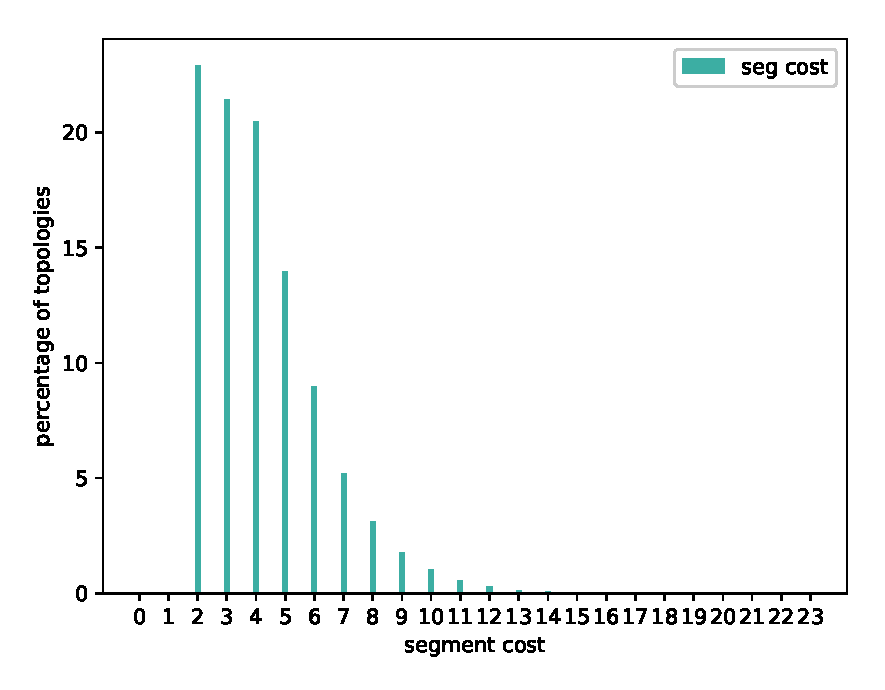
\includegraphics[width=.85\columnwidth]{./Network-lib/data/plot/minCostEDP_segcost.eps}
\end{center}
\caption{Distribution of the maximum segment of maximum cardinality sets of disjoint paths with total minimum latency.}
\label{fig:minCostEDP_segcost}
\end{figure}

\subsection{Maximum set of disjoint sr-paths}

We propose two MIP models for adapting the graph model $\maxedp(G, s, t)$ to Problem \ref{prob:max-sr-edp}. We start by defining
an indicator function telling use whether an edge belongs to the shortest paths between two given nodes.
That is, let $I$ to denote a function $V(G)^2 \times E(G) \rightarrow \{0, 1\}$ defined such that $I(u, v, e) = 1$ if and only if $e \in E(\sp(u, v))$.

Our first model is an adaptation of the traffic engineering segment model $\srteseg(G, \mathcal{D})$ proposed in Chapter \ref{chapter:te}. 
Our demand set contains unit demands between $s$ and $t$. Each such demand corresponds to a sr-path that is edge-disjoint from the
others. We can select the number of demands to be equal to the out-degree of $s$, since this is an upper bound on the number
of disjoint paths from $s$ to any other node. Our objective will by to route a maximum
amount of demands in a way such that no two demands are routed over the same edge. We use variables $x^d_{uv}$ 
saying whether $\sp(u, v)$ is used by the sr-path corresponding to demand $d$. We replace the capacity constraints
by disjointness constraints which consists of requiring that for each edge, at most one demand is routed over it. The rest of the model
is the same as $\srteseg(G, \mathcal{D})$ which uses flow constraints to ensure that paths go from $s$ to $t$.

\begin{center}
\begin{tabular}{rcllr}
\multicolumn{5}{l}{$\sredpseg(G, s, t)$} \\[0.5cm] 
\multicolumn{3}{l}{$\mathbf{max} \quad \displaystyle \sum_{u \in V(G)} \sum_{d = 1}^r x^d_{su}$} & $\textbf{s.t.}$ & \\[0.5cm]
%\multicolumn{5}{l}{{\color{gray!80!white} qsdqsd qsdqsaz sqd s dazz azeqsd azee aze qsd }} \\
$\displaystyle \sum_{d = 1}^r \sum_{u \in V(G)} \sum_{v \in V(G)}  x^d_{uv} \cdot I(u, v, e)$ & $\leq$ & $1$ & $\forall e \in E(G)$ & \\[0.5cm]
$\displaystyle \sum_{u \in V(G) \setminus \{ v \}} x^d_{uv} - \sum_{u \in V(G) \setminus \{ v \}} x^d_{vu}$ & $=$    &  $0$ & $\forall d$, & \\[-0.2cm]
& & & $\forall v \in V(G) \setminus \{ s, t \}$ & \\[0.5cm]
$\displaystyle \sum_{d = 1}^r \sum_{u \in V(G) } x^d_{us} + x^d_{tu}$ & $=$    &  $0$ & $\forall d \in \{1, \ldots, |\oute(s)|\}$ \\[0.5cm] 
$\displaystyle \sum_{u \in V(G)} \sum_{v \in V(G)} x^d_{uu}$ & $\leq$    &  $k$ & $\forall d \in \{ 1, \ldots, |\oute(s)| \}$, \\[0.5cm]
$x^d_{uv}$  &    $\in$    &  $\{0, 1\}$  & $\forall e \in E(G),$ & \\
  &    &   & $\forall d \in \{1, \ldots, |\oute(s)|\}$ &
\end{tabular}
\end{center}

Next, we propose another model whose original idea is due to
Bernard Fortz. After we will compare both models. Note that both these models only support node segments
in the sr-paths.

%For simplicity, we start by presenting the model for sr-paths consisting
%only on node segments. We will describe later how to extend it to also take into account
%adjacency segments as well. 
%As it was already observed by Renauld Hartert, a sr-path 
%consisting only on node segments can between seen as a path on the complete graph
%with $V(G)$ nodes. The correspondence is quite clear as a sr-path with only node segments
%is a sequence $\langle x_1, \ldots, x_l \rangle$ such that each $x_i \in V(G)$ and a
%path on the complete graph also is a sequence $(v_1, \ldots, v_r)$ with each $v_i \in V(G)$.
A sr-path with only node segments is a sequence $\langle y_1, \ldots, y_l \rangle$
such that each $y_1, \ldots, y_l \in V(G)$. The idea behind Fortz  model is to define binary variables 
$x^i_{uv}$ such that $x^i_{uv} = 1$ if and only if
$u$ and $v$ appear as consecutive segments $y_i = u$ and $y_{i + 1} = v$ of a sr-path used in the solution.
These variables are defined for $i = 1, \ldots, k - 1$ where $k$ is the maximum segment cost that we
want to allow the paths to have. Consider for instance that we have a solution where
$x^1_{sa} = x^2_{ab} = x^3_{bt} = 1$. This will correspond to using the sr-path $\langle s, a, b, t\rangle$
as shown in Figure \ref{fig:modelfortz}. So, basically, the index $i$ is saying the position at which we use
each segment.
Note that a more intuitive model would be to drop the $i$ index and use variables $x_{uv}$ to mean that we use
the shortest paths between $u$ and $v$ to route traffic. By adding flow conservation constraints similar to the
ones used in model $\maxflow(G, s, t)$ we can make sure that these variables actually come together
to constitute sr-paths. However, this gives no way of restricting the segment cost of those paths.


\begin{figure}
\begin{center}
\begin{tikzpicture}
\draw[gray, dashed] (0, 0) -- (0, 5) node[anchor=south] {$i = 1$};
\draw[gray, dashed] (2, 0) -- (2, 5) node[anchor=south] {$i = 2$};
\draw[gray, dashed] (4, 0) -- (4, 5) node[anchor=south] {$i = 3$};
\draw[gray, dashed] (6, 0) -- (6, 5) node[anchor=south] {$i = 4$};
\node[scale=0.15] (s) at (-1, 2.5) {\router{s}{router}};
\node[scale=0.15] (a) at (1, 4) {\router{$a$}{router}};
\node[scale=0.15] (b) at (3, 3.5) {\router{$b$}{router}};
\node[scale=0.15] (t1) at (5, 3.75) {\router{$t$}{router}};

\node[scale=0.15] (c) at (1, 5 - 4 - 0.5) {\router{$c$}{router}};
\node[scale=0.15] (d) at (3, 5 - 3.5 - 0.5) {\router{$d$}{router}};
\node[scale=0.15] (e) at (5, 5 - 3.75 - 0.5) {\router{$e$}{router}};
\node[scale=0.15] (t2) at (7, 2.5) {\router{$t$}{router}};


\draw (s) edge[line width=2, above, sloped, ->] node {\small $x^1_{s a} = 1$} (a);
\draw (a) edge[line width=2, above, sloped, ->] node {\small $x^2_{a b} = 1$} (b);
\draw (b) edge[line width=2, above, sloped, ->] node {\small $x^3_{b t} = 1$} (t1);

\draw (s) edge[line width=2, above, sloped, ->] node {\small $x^1_{s c} = 1$} (c);
\draw (c) edge[line width=2, above, sloped, ->] node {\small $x^2_{c d} = 1$} (d);
\draw (d) edge[line width=2, above, sloped, ->] node {\small $x^3_{d e} = 1$} (e);
\draw (e) edge[line width=2, above, sloped, ->] node {\small $x^4_{e t} = 1$} (t2);

\node[right = 0.1cm of t2] {$\langle s, c, d, e, t \rangle$};
\node[right = 0.1cm of t1] {$\langle s, a, b, t \rangle$};
\end{tikzpicture}
\end{center}
\caption{Two examples of how the variables $x^i_{uv}$ define sr-paths.}
\label{fig:modelfortz}
\end{figure}

\begin{center}
\begin{tabular}{crcllr}
\multicolumn{5}{l}{$\sredpfortz(G, s, t)$} \\[0.5cm] 
$\displaystyle \mathbf{max}$ & $\displaystyle \sum_{u \in V(G)} x^1_{su}$ & & & & \\[0.5cm]
$\textbf{s.t.}$ & $\displaystyle \sum_{i = 1}^k \sum_{u \in V(G)} \sum_{v \in V(G)} I(u, v, e) \cdot x^i_{uv} $ & $\leq$    & $1$ & $\forall e \in E(G)$  & $(1)$ \\[0.5cm]
                & $\displaystyle \sum_{v \in V(G)} x^{i - 1}_{vu} - \sum_{v \in V(G)} x^i_{uv}$ & $=$ & $0$ & $\forall u \in V(G) \setminus \{s, t\}$, &  $(2)$ \\[-0.2cm] 
                & & & & $i = 2, \ldots, k$ &  \\[0.5cm] 
                & $\displaystyle \sum_{i = 1}^k \sum_{v \in V(G)} x^i_{vs} + x^i_{tv}$ & $=$ & $0$ &  & $(3)$ \\[0.5cm]
                & $\displaystyle \sum_{v \in V(G) \setminus \{s\}} x^1_{vu} + \sum_{v \in V(G) \setminus \{t\}} x^k_{uv}$ & $=$ & $0$ & $\forall u \in V(G)$ & $(4)$\\[0.5cm]
                & $x_{e}$ & $\in$ & $\mathbb{N}$
\end{tabular}
\end{center}

Constraints $(1)$ ensure that each edge is used only once making sure that the final paths are indeed edge-disjoint. Recall that setting $x^{i - 1}_{uv}$ to $1$ means that
node $u$ is used as a node segment at position $i - 1$ in some sr-path in the solution. Thus, if $u \neq t$ we need to make sure that there is also some node $v'$ coming after $u$ in this sr-path as
illustrated in Figure \ref{fig:modelfortz2}. This is what constraints $(2)$ ensure, that is, that for each $u$ such that $x^{i - 1}_{vu}$ for some $v$, there is also some element
$v'$ such that $x^{i}_{uv'}$ ensuring that the path does not end at a node $u \neq t$. 
These constraints are similar to the classical conservation constraints that are commonly used in these kinds of models to ensure connectivity.



\begin{figure}
\begin{center}
\begin{tikzpicture}
\draw[gray, dashed] (1, 1) -- (1, 4) node[anchor=south] {$i - 1$};
\draw[gray, dashed] (4, 1) -- (4, 4) node[anchor=south] {$i$};
\node[scale=0.15] (v) at (-0.5, 2.5) {\router{$v$}{router}};
\node[scale=0.15] (u) at (2.5, 2.5) {\router{$u$}{router}};
\node[scale=0.15] (v2) at (5.5, 2.5) {\router{$v'$}{router}};

\draw (v) edge[line width=2, above, sloped, ->] node {\small $x^{i - 1}_{uv} = 1$} (u);
\draw (u) edge[line width=2, above, sloped, ->] node {\small $x^{i}_{uv'} = 1$} (v2);

\end{tikzpicture}
\end{center}
\caption{If $x^{i - 1}_{uv} = 1$ .}
\label{fig:modelfortz2}
\end{figure}

Constraints $(3)$ simply make sure that $s$ appears only as the first element of the sr-paths and that $t$ occurs only as the last one.
Finally, constraints $(4)$ prevent other nodes to be the starting and end-points of paths by ensuring that $x^1_{uv}$ can only be set if $u = s$
and that $x^k_{uv}$ can only be set if $v = t$.

Figure \label{fig:maxEDP_runtime} shows a CDF of the runtime needed to compute optimal solutions of $\sredpseg(G, s, t)$  and $\sredpfortz(G, s, t)$ using Gurobi. In
both cases the maximum number of segments was set to $5$. We generated
$100$ random source-destination pairs and solved both models over these pairs for all instances in our dataset. We can see (in orange) that the segment
model is slower than the model proposed by Fortz (in blue). We see that the maximum runtime of the Fortz model is about $3$ minutes whereas
the maximum runtime of the segment model is about $10$ minutes. In both cases this shows that using a MIP solver for computing sets of disjoint
sr-paths is feasible in practice in a reasonable amount of time. 
In order to try to understand whether our sample of $100$ pairs is large enough, we computed a box-plot of the run times on the topologies from groups
\texttt{real} and \texttt{rf} of the Fortz model. 
We selected these because they are the largest ones and we cannot show all results in the box plot. Figure \ref{fig:maxEDP_boxplot} shows these. Except for
topology \texttt{1239}, the runtime does not have a high variance so we can expect that the average runtime is close
to the one computed.

\begin{figure}
\begin{center}
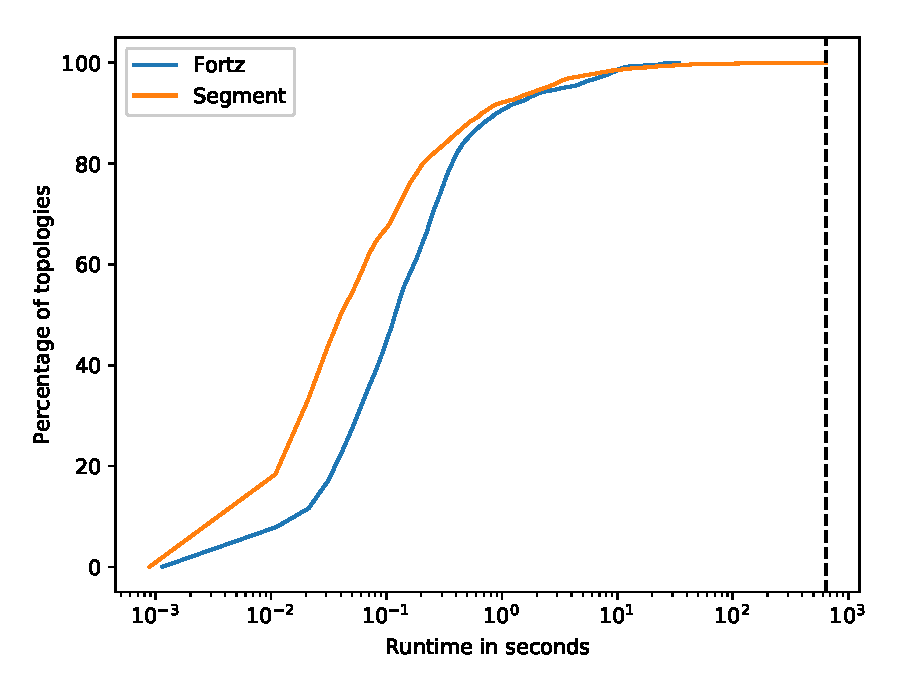
\includegraphics[width=.85\columnwidth]{./Network-lib/data/plot/maxEDPMip_runtime_both.eps}
\end{center}
\caption{CDF over all topologies of the runtime for solving $\sredpseg(G, s, t)$ and $\sredpfortz(G, s, t)$ over $100$ randomly selected source-destination pairs.}
\label{fig:maxEDP_runtime}
\end{figure}

\begin{figure}
\begin{center}
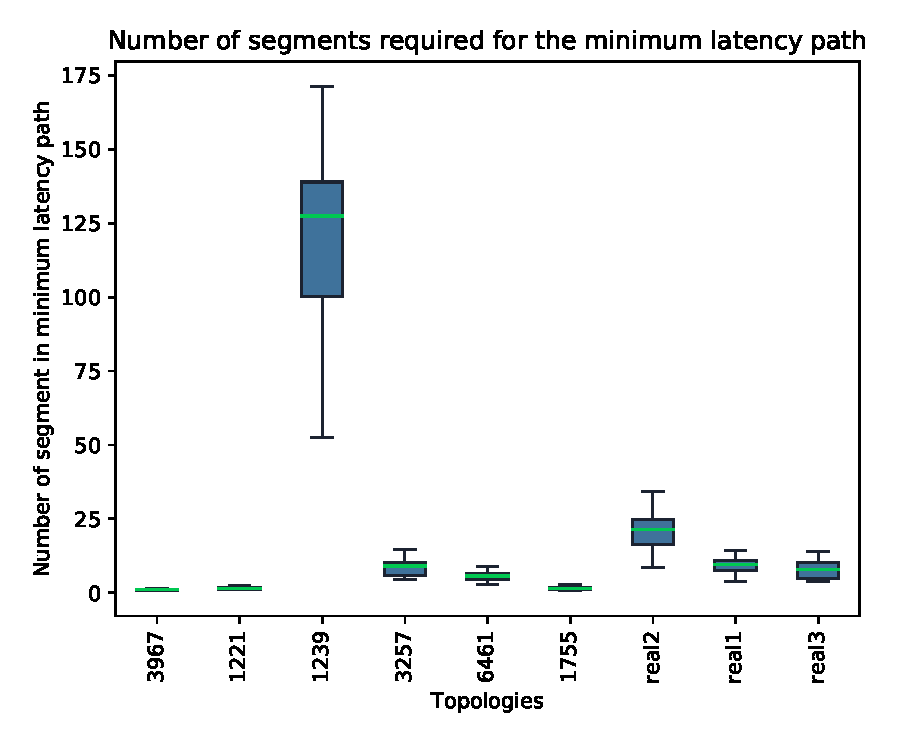
\includegraphics[width=.85\columnwidth]{./Network-lib/data/plot/maxEDP_boxplot.eps}
\end{center}
\caption{CDF over all topologies of the runtime for solving $\sredpfortz(G, s, t)$ over $100$ randomly selected source-destination pairs.}
\label{fig:maxEDP_boxplot}
\end{figure}

We also analyzed how restrictive the segmentation constraints with respect to the existence of disjoint paths.
For this we computed the difference between the maximum number of disjoint paths between the sources and the destinations
with the maximum number of disjoint sr-paths of segment cost at most $5$. Whenever this difference is $0$ we know that
requiring the path to be implementable with a segment cost of at most $5$ posed no restrictions in finding solutions.
Table \ref{tab:nbp_vs_seg} shows these results. We can see that for $95\%$ of the pairs the segmentation constraints were
not restrictive. This indicates that with about $5$ segments we can implement sets of sr-paths that are as large as the
theoretical maximum supported on the graph topology.

\begin{figure}
\begin{center}
\begin{tabular}{rccccc}
\toprule
difference & $0$ & $1$ & $2$ & $3$ & $\geq 4$ \\
\midrule
percentage of $s$-$t$           & 95\% & 4\% & 0.4\% & 0.1\% & 0.5\%
\end{tabular}
\end{center}
\caption{Percentage of pairs for each value of the difference between the maximum number of disjoint paths and maximum number of disjoint sr-paths with segment
cost at most $5$.}
\label{tab:nbp_vs_seg}
\end{figure}

\subsection{Minimizing the total latency}

For both models it is straightforward to modify the models to minimize the total latency of the sr-paths.
In both cases we need to first compute the maximum number of disjoint sr-paths that exist between the source
and destination, say $P$. Then, we need to replace the objective function by a minimization function that
adds all latencies together. We also need an additional constraint requiring the total number of paths in the solution to be equal to $P$.
Concretely, in the segment model, $\sredpseg(G, s, t)$, we can obtain this by replacing the objective function by
$$
\textbf{minimize} \quad \sum_{d = 1}^r \sum_{u \in V(G)} \sum_{v \in V(G)} \lat(u, v) \cdot x^d_{uv} 
$$
and adding a constraint
$$
\sum_{u \in V(G)} \sum_{d = 1}^r x^d_{su} = P. 
$$
For the Fortz model, $\sredpfortz(G, s, t)$, the change is analogous. The objective function
becomes 
$$
\textbf{minimize} \quad \sum_{i = 1}^k \sum_{u \in V(G)} \sum_{v \in V(G)} \lat(u, v) \cdot x^i_{uv} 
$$
and we add a constraint requesting $P$ paths starting at the source $s$:
$$
\sum_{u \in V(G)} x^1_{su} = P. 
$$

%\todo{Add plot comparing the runtime of minimizing latency vs not.}

\section{Min-max edge-disjoint sr-paths}

We now focus on the problem of computing pairs of disjoint paths with a min-max objective function. More
specifically, we aim at connecting via disjoint sr-paths a source node 
$s_1$ to a destination $t_1$ and a source node $s_2$ to a destination $t_2$
such that the maximum latency among those two paths is as small as possible.

\begin{problem}{Min-max edge-disjoint sr-paths}
\label{prob:disjointsrp}
\textbf{Input:} A network $G$ and $s_1, s_2, t_1, t_2 \in V(G)$ such that $s_1 \neq t_1$ and $s_2 \neq t_2$
and $k \in \mathbb{N}$.

\textbf{Output:} Two disjoint sr-paths $\sr{p}_1 \in \Pk(s_1, t_1), \sr{p}_2 \in \Pk(s_2, t_2)$ such that
$$
\max (\lat(\sr{p}_1), \lat(\sr{p}_2))
$$
is minimal.
\end{problem}

As we mentioned in the previous section, this problem is \NPhard \cite{minmax-disjoint-90, Li1990}.

\subsection{MIP formulation}

We saw above that Fortz model performed better than the segment model for computing maximal sets of disjoint paths.
However it is hard to enforce a source to destination assignment with this model. The reason is that different paths are not
modeled explicitly. For this reason, we use the segment model for solving Problem \ref{prob:disjointsrp}. With the segment model
each path is encoded in the index $d$ of the variables $x^d_{uv}$. This makes it easy to for the path starting at $s_1$ to end at $t_1$ and the
path starting at $s_2$ to end at $t_2$. The adapted model is the following.

\begin{center}
\begin{tabular}{rcllr}
\multicolumn{5}{l}{$\sredp(G, s_1, s_2, t_1, t_2)$} \\[0.5cm] 
\multicolumn{3}{l}{$\mathbf{min} \quad \lambda$} & $\textbf{s.t.}$ & \\[0.5cm]
$\displaystyle \sum_{d = 1}^2 \sum_{u \in V(G)} \sum_{v \in V(G)}  x^d_{uv} \cdot I(u, v, e)$ & $\leq$ & $1$ & $\forall e \in E(G)$ & \\[0.5cm]
$\displaystyle \sum_{u \in V(G) \setminus \{ v \}} x^d_{uv} - \sum_{u \in V(G) \setminus \{ v \}} x^d_{vu}$ & $=$    &  $0$ & $\forall d \in \{1,2\}$, $\forall v \in V(G) \setminus \{ s_d, t_d \}$ & \\[0.5cm]
$\displaystyle \sum_{u \in V(G)} \sum_{v \in V(G)} \lat(u, v) \cdot x^d_{u, v}$ & $\leq$    & $\lambda$ & $\forall d \in \{ 1, 2 \}$ \\[0.5cm]
$\displaystyle \sum_{u \in V(G) \setminus \{ s_d \}} x^d_{s_d u}$ & $=$    & $1$ & $\forall d \in \{ 1, 2 \}$ \\[0.5cm]
$\displaystyle \sum_{u \in V(G) \setminus \{ t_d \}} x^d_{u t_d}$ & $=$    & $1$ & $\forall d \in \{ 1, 2 \}$ \\[0.5cm]
$\displaystyle \sum_{d = 1}^2 \sum_{u \in V(G)} x^d_{u s_d} +  x^d_{t_d u}$ & $=$    & $0$ & $\forall d \in \{ 1, 2 \}$ \\[0.5cm]
$\displaystyle \sum_{u \in V(G)} \sum_{v \in V(G)} x^d_{uu}$ & $\leq$      & $k$ & $\forall d \in \{ 1, 2 \}$ \\[0.5cm]
$x^d_{uv}$  &    $\in$    &  $\{0, 1\}$  & $\forall e \in E(G), \ \forall d \in \{1, 2 \}$ & \\[0.5cm]
$\lambda$   &    $\geq$   & $0$ & &
\end{tabular}
\end{center}


\subsection{Dedicated algorithm}

We also proposed a dedicated algorithm for solving this problem. This was actually our original idea that was published in CoNEXT 18 \cite{rdp}.
However we will see that it is actually less efficient and flexible than the MIP formulation.
Recall that in our definition of network, we mentioned that each edge is indexed with a unique number between $0$ and $|E(G)| - 1$. This is useful for
defining parallel edges. These indexes are also important in the context of disjoint paths. From an implementation point of view, we will represent the
set of edges corresponding to a sr-path $\sr{p}$, $E(\sr{p})$, as a \emph{bitset} $b$ such that $b_i = 1$ if and only if edge with $\idx(e) = i$ belongs
to $E(\sr{p})$.

Bitsets are a very simple and efficient way to represent subsets of $\{ 0, \ldots, n - 1 \}$ for some fixed, not too large value of $n$. Conceptually they
are similar to an array of booleans of size $n$. However, a bitset is represented instead (on a 64-bit machine) with an array of \texttt{long}. Each element of the array
represents a group of $64$ boolean values with its bits. So the bits of the first element in the array will represent elements $0$ to $63$, the second $64$ to $127$ and 
so forth. Figure \ref{fig:bitset} illustrates a bitset for $n = 512$. In this example, element $131$ is represented by the forth bit of
the third long.

\begin{figure}
\begin{center}
\begin{tikzpicture}

\draw[green, ultra thick] (4.2, 0) -- (4.2, 1);


\draw[dashed, gray] (2, -0.5) -- (2, 1.5);
\draw[dashed, gray] (4, -0.5) -- (4, 1.5);
\draw[dashed, gray] (6, -0.5) -- (6, 1.5);
\draw[dashed, gray] (8, -0.5) -- (8, 1.5);

\fill[green] (3.5, -2) rectangle (4, -1.5);

\draw[gray, ultra thick, dotted] (4, 0) -- (2, -1.5);
\draw[gray, ultra thick, dotted] (6, 0) -- (8, -1.5);

\draw[step=2] (0, 0) grid (10, 1);
\draw (0, 0) rectangle (10, 1);

\draw[step=0.5] (2, -2) grid (4.5, -1.5);
\draw (2, -2) rectangle (4.5, -1.5);

\draw[step=0.5] (5.5, -2) grid (8, -1.5);
\draw (5.5, -2) rectangle (8, -1.5);

\node at (5, -1.75) {$\ldots$};

\node at (2.25, -1.25) {0};
\node at (2.75, -1.25) {1};
\node at (3.25, -1.25) {2};
\node at (3.75, -1.25) {3};
\node at (4.25, -1.25) {4};


\node at (2.25, -2.25) {128};
\node at (2.25 + 1.5, -2.25) {131};

\node at (5.5 + 2.25, -2.25) {255};

\node at (5.5 + 0.25, -1.25) {59};
\node at (5.5 + 0.75, -1.25) {60};
\node at (5.5 + 1.25, -1.25) {61};
\node at (5.5 + 1.75, -1.25) {62};
\node at (5.5 + 2.25, -1.25) {63};

\node at (0.1, 1.2) {0};
\node at (1.75, 1.2) {63};

\node at (2.25, 1.2) {64};
\node at (3.65, 1.2) {127};

\node at (4.35, 1.2) {128};
\node at (5.65, 1.2)  {255};

\node at (6.35, 1.2) {256};
\node at (7.65, 1.2) {383};

\node at (8.35, 1.2) {384};
\node at (9.7, 1.2) {511};

\node at (1, 0.5) {long 1};
\node at (3, 0.5) {long 2};
\node at (5, 0.5) {long 3};
\node at (7, 0.5) {long 4};
\node at (9, 0.5) {long 5};

\end{tikzpicture}
\end{center}
\caption{Representation of a bitset with $n = 512$.}
\label{fig:bitset}
\end{figure}

The advantage of this representation over a boolean array representation is that each set operation on a long can be performed in $O(1)$.
So for example, to compute the intersection between two bitsets we simply need to loop over the array and perform a bitwise and between
corresponding elements. Therefore we only need to perform $n \slash 64$ operations rather $n$. Even though in big-Oh notation this sill yields
the same complexity, $O(n)$, the runtime in practice is $64$ times faster which is a gigantic speedup.
Using a bitset representation for the set of edges of a sr-path we can then perform set operations over these very efficiently. 

In particular, this representation makes it possible to very efficiently check whether or not two sr-paths are disjoint. We exploit this to
design an algorithm for solving \ref{prob:disjointsrp}. Given a sr-path $\sr{p}_1$ we can find the minimum latency sr-path $\sr{p}_2$ that
is disjoint from it in polynomial time by using the minimum latency sr-path algorithm from Chapter \ref{chapter:sr-optimal}. We simply need to
adapt it so that it avoids $E(\sr{p}_1)$. To do so, we need to know the set of edges in all sr-paths of the form $\langle x, y \rangle$
where $x, y \in V(G)$. We show how to do this in the next.

\subsubsection{Pre-computing the forwarding graphs}

\begin{lemma}
\label{lemma:forwdp}
Let $G$ be a network and $x, y \in V(G)$. Then
\begin{equation}
\label{eq:forwdp}
E(\sp(x, y)) = \bigcup_{ e \in \ine(\sp(x), y) } E(\sp(x, e^1)) \cup \{ e \}.
\end{equation}
\end{lemma}

\begin{proof}
$(\subseteq)$ Let $e \in E(\sp(x, y))$. Let $p = (e_1, \ldots, e_n)$ be a shortest path from $x$ to $y$ 
passing by $e$. Then $e = e_i$ for some $i$.  Note that $(e_1, \ldots, e_{n - 1})$ 
is a shortest path from $x$ to $e^2_{n - 1} = e^1_n$ and, since $e^2_n = y$, 
$e_n \in \ine(\sp(x), y)$. Thus, if $i = n$ then $e$ clearly belongs to the right-hand
side of (\ref{eq:forwdp}). Otherwise, if $i < n$ then $e$ belongs to the shortest 
path $(e_1, \ldots, e_{n - 1})$ from $x$ to $e^2_{n - 1} = e^1_n$. Since $e_n \in
\ine(\sp(x), y))$ we again conclude that $e$ belongs to the rhs of (\ref{eq:forwdp}).

$(\supseteq)$ Let $e$ be a edge belonging to the rhs of (\ref{eq:forwdp}). There exists
$f \in \ine(\sp(x), y))$ such that either $e = f$ or $e \in E(\sp(x, f^1))$. If $e = f$
then $e = f \in \ine(\sp(x), y)) = \ine(\sp(x, y))$ so it belongs to $\sp(x, y)$. Otherwise,
$e$ belongs to a shortest path from $x$ to the origin of $f$. Since $f \in \ine(\sp(x), y)$
we have that $\dist(x, y) = \dist(x, f^1) + \igp(f)$. Since $e$ belongs to a shortest
path $p$ from $x$ to $f^1$, we have 
$\dist(x, e^1) + \igp(e) + \dist(e^2, f^1) = \dist(x, f^1) = \igp(p)$.
Then
\begin{align*}
\dist(x, y) & = \dist(x, f^1) + \igp(f) \\
& = \dist(x, e^1) + \igp(e) + \dist(e^2, f^1) + \igp(f) \\
& = \dist(x, e^1) + \igp(e) + \dist(e^2, f^2) \\
& = \dist(x, e^1) + \igp(e) + \dist(e^2, y) \\
\end{align*}
so that $e \in \sp(x, y)$.
\end{proof}

Using Lemma \ref{lemma:forwdp} we can leverage the speed of bitsets to
efficiently compute $E(\SP(v, u))$ for all $u, v \in V(G)$. Note that we
could always compute them using the definition, that is, computing 
$\sp(u)$ for all $u$ and then for each $v$ using a breath-first search to
extract the subset of edges of $\sp(u)$ that belong to $\sp(u, v)$. 
Using equation (\ref{eq:forwdp}), we can compute $E(\sp(u, v))$ by
performing $|\ine(\sp(u), v)|$ bitset operations. As we mentioned above,
in theory this is not faster but it practice it runs faster even due to the
usage of bitsets. However, in the next section we will see that applying the same idea
to precompute another kind of data that we will need leads to huge gains in
runtime. Algorithm \ref{algo:preforw} shows how we can easily compute this recurrence.
For each $u$ we compute the shortest path subnetwork rooted at $u$ and then compute
a topological order $v_1, v_2, \ldots, v_n$ to compute $E(\sp(u, v_i)$ in an order such
that when computing $E(\sp(u, v_i))$ we already computed $E(\sp(u, e^1))$ for all $e \in
\ine(\sp(u), v_i)$.

%as shown in Figure \ref{fig:precompute_forw_runtime}.

%\begin{figure}
%\begin{center}
%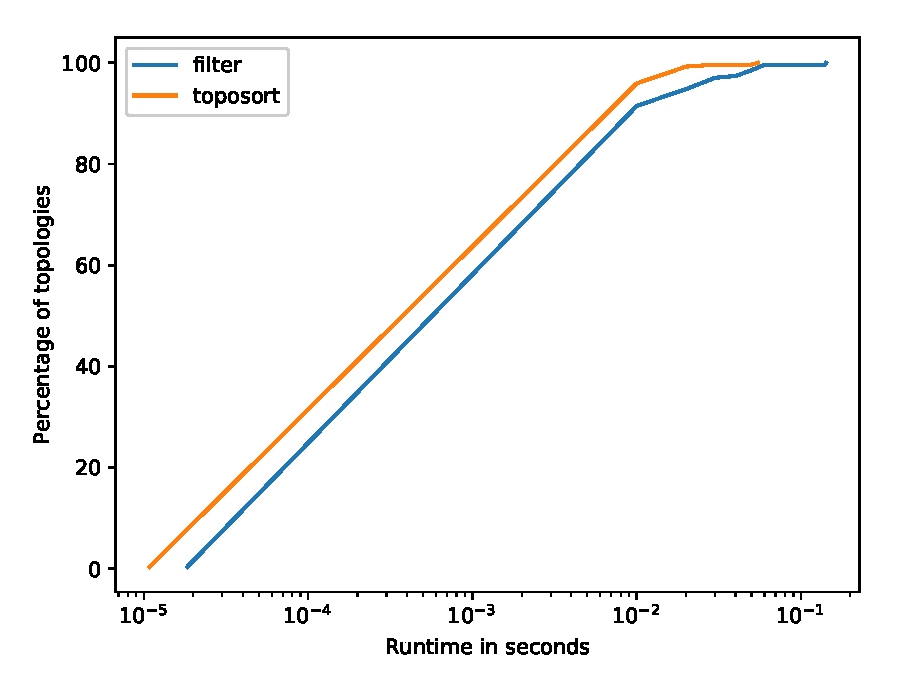
\includegraphics[width=.85\columnwidth]{./Network-lib/data/plot/precompute_forw_runtime.eps}
%\end{center}
%\caption{todo}
%\label{fig:precompute_forw_runtime}
%\end{figure}

\begin{algorithm}[t]
\small
\caption{$\textsf{precompute-forwEdges}\left( g \right)$}
\begin{algorithmic}[1]
\FOR{$u, v \in V(G)$}
  \STATE $fwe(u, v) \gets \textsf{Bitset}()$
\ENDFOR
\FOR{$u \in V(G)$}
  \STATE $\sp(u) \gets \textsf{dikstra-dag}(g, u)$
  \STATE $order \gets \textsf{toposort}(\sp(u))$
  \FOR{$v \in order$}
    \FOR{$e \in \ine(\sp(u), v)$}
      \STATE $fwe(u, v) \gets fwe(u, e^1) \cup \{ e \}$
    \ENDFOR
  \ENDFOR
\ENDFOR
\RETURN $fwe$
\end{algorithmic}
\label{algo:preforw}
\end{algorithm}

Having pre-computed $E(\sp(u, v))$ we can easily adapt Algorithm
\ref{algo:min_weight_sr_path} to make sure that the path that is computed avoids all
edges in $E(\sr{p}_1)$. Recall that, according to Chapter \ref{chapter:sr-optimal}, 
the recurrence for the minimum latency path
from $s_2$ to $v$ with segment cost at most $i$ will be

\[\mathit{sol}(i, v) = \min \left\{
  \begin{matrix}
    \mathit{sol}(i - 1, v) &  \\[0.2cm]
    \mathit{sol}(i - 1, u)  +  \lat(u, v)  & \textbf{s.t} \text{ $u \in V$} \\[0.2cm]
    \mathit{sol}(i - 2, r)  +  \lat(r, e^1) + \lat(e) & \textbf{s.t} \text{ $u \in V, e \in \ine(v)$} \\
\end{matrix}
  \right.
\]

as illustrated by Figure \ref{fig:dp_disjoint}. In order to guarantee disjointness,
we just need to ensure that for each case all pieces are disjoint
from $\sr{p}_1$. This means ensuring that 
$$
E(\sp(u, v)) \cap E(\sr{p}_1) = \emptyset
$$
in the second case and that 
$$\left( E(\sp(u, e^1)) \cup \{ e \} \right) \cap E(\sr{p}_1) = \emptyset
$$
in the third case. In term of algorithms, this corresponds to adding these conditions
to lines \ref{mwsrp-if1} and \ref{mwsrp-if2} from Algorithm \ref{algo:min_weight_sr_path}, respectively. Note that these changes will
have a minor impact over the overall performance of the algorithm since we use bitsets
to compute these intersections and $E(\sp(u, v))$ is given as input for all $u, v \in V(G)$.

 \begin{figure}
 \begin{center}
 \begin{tikzpicture}
 \node[scale=0.15] (s) at (0, 0) {\router{$s_2$}{router}};
 \node[scale=0.15] (x) at (5+2, 0) {\router{v}{router}};
 \node[scale=0.15] (y) at (2+2, 0) {\router{u}{router}};
 \node[scale=0.15] (z) at (4+2, -2) {\router{u}{router}};
 \node[scale=0.15] (r) at (2+1, -2-0.2) {\router{r}{router}};
 
 
 
 \draw (s) edge[very thick, below, bend right=10, dashed, ->] node {$\mathit{sol}(i - 1, v)$} (y);
 \draw (y) edge[very thick, bend right=10, dashed, ->, below] node {$\lat(u, v)$} (x);
 \draw (s) edge[very thick, bend left=40, dashed, ->, above] node {$\mathit{sol}(i - 1, v)$} (x);
 %\draw (s) edge[very thick, bend right=30, dashed, ->] (z);
 \draw (z) edge[very thick, ->, sloped, below] node {$\lat(e)$} (x);
 
 \draw (s) edge[very thick, bend right=30, dashed, ->, below, sloped] node {$\mathit{sol}(i - 2, r)$} (r);
 \draw (r) edge[very thick, bend right=20, dashed, ->, below, sloped] node {$\lat(u, e^1)$} (z);
 
 \end{tikzpicture}
 \end{center}
 \caption{Illustration of the $\mathit{sol}$ recurrence}
 \label{fig:dp_disjoint}
 \end{figure}

In order to find a pair of paths, we perform a depth-first search on $\sr{p}_1$ and use
the above algorithm to maintain the minimum latency sr-path $\sr{p}_2$ that is disjoint from the 
current partial path $\sr{p}_1$. At each step of the search, we try to extend $\sr{p}_1$
with either a node segment or an adjacency segment. We perform the following steps to
avoid exploring useless extensions of $\sr{p}_1$. Let $\sr{p}_1 = \langle
x_1, \ldots, x_n \rangle$ be the partial path at given search node, $\sr{p}_2$
the minimum latency sr-path disjoint from the partial path $\sr{p}_1$, $l^*$ the 
latency of the best solution found so far and $x$ be a node or adjacency segment:

\begin{itemize}
 \item Let $v = x^2_n$ be the node where $\sr{p}_1$ ends. In the best case, the latency
 of the completed sr-path $\sr{p}_1$ will be its current latency plus the latency of the minimum
 latency path between $v$ and $t_1$ in $G$. Let's denote that latency by $\mathcal{L}(v, t_1)$.
 Therefore, if $\max(\lat(\sr{p}_1) + \mathcal{L}(v, t_1), \lat(\sr{p}_2)) \geq l^*$
 we can stop the search since we will never reach a better solution.
 
 \item By Theorem \ref{thm:sracyclic}, there is
 a solution to Problem \ref{prob:disjointsrp} where both $\sr{p}_1$ and $\sr{p}_2$ are acyclic.
 Hence, we can ignore $x$ if $\sr{p}_1 \oplus x$ is cyclic. Checking this can be 
 done efficiently thanks to our bitset representation and forwarding graph
 edge set pre-computation.
 
 \item If $\sr{p}_1 \oplus x$ does not intersect 
 $\sr{p}_2$ then $\sr{p}_2$ remains the minimum latency sr-path that is disjoint from
 $\sr{p}_1 \oplus x$ so there is not need to re-compute it. Otherwise, we use the algorithm
 that we described above to compute a new minimum latency sr-path $\sr{p}_2$. If this path does
 not exist, then it is fruitless to try $x$ as an extension of $\sr{p}_1$.
 
 \item If there does not exist a pair of disjoint paths
 on $G$, one from $x^2$ to $t_1$ and another from $s_2$ to $t_2$ then we will never reach a 
 solution by extending $\sr{p}_1$ with $x$. However, we have seen that checking whether
 such disjoint paths exists is \NPcomplete. We use a relaxation of this condition by allowing
 the path from $x^2$ to go to $t_2$ or the path from $s_2$ to go to $t_1$ which is equivalent
 to checking whether the maximum flow between $\{x^2, s_2\}$ and $\{t_1, t_2\}$ is
 at least $2$.
\end{itemize}

By putting all these ideas together we can formally express Algorithm
\ref{algo:disjoint_srp} and \ref{algo:disjoint_srp_dfs} for solving Problem
\ref{prob:disjointsrp}.

\begin{algorithm}[t]
\small
\caption{$\textsf{disjoint-srpaths}\left( g, s_1, s_2, t_1, t_2 \right)$}
\begin{algorithmic}[1]
\STATE $\sr{p}_2 \gets \textsf{min-lat-disjoint-srpath}(s_2, t_2, k)$
\STATE $l^* \gets \infty$
\FOR{$x \in V(G) \cup E(g)$}
  \STATE $\textsf{disjoint-srpaths-dfs}\left( \langle x \rangle, \sr{p}_2 \right)$
\ENDFOR
\IF{$l^* = \infty$}
  \RETURN \textbf{null}
\ENDIF
\RETURN $\sr{p}^*_1, \sr{p}^*_2$
\end{algorithmic}
\label{algo:disjoint_srp}
\end{algorithm}

\begin{algorithm}[t]
\small
\caption{$\textsf{disjoint-srpaths-dfs}\left( \sr{p}_1, \sr{p}_2 \right)$}
\begin{algorithmic}[1]
\IF{$\max(\lat(\sr{p}_1) + \mathcal{L}(\sr{p}_1.\textsf{dest}(), t_1) \geq l^*$} 
  \RETURN
\ENDIF
\cmtline{we reached here so if the path is complete, it is a better solution}
\IF{$\sr{p}_1.\textsf{dest}() = t_1$}
  \STATE $l^* \gets \max(\lat(\sr{p}_1), \lat(\sr{p}_2))$
  \STATE $\sr{p}^*_1, \sr{p}^*_2 \gets \sr{p}_1, \sr{p}_2$
  \RETURN
\ENDIF
\cmtline{try extend $\sr{p}_1$ with a node segment}
\IF{$\cost(\sr{p}_1) + 1 > k$}
  \RETURN
\ENDIF
\FOR{$u \in V(G)$}
  \cmtline{check whether we can cut with min cost flow}
  \STATE $P, l \gets \textsf{min-cost-flow}(g, \{u, s_2\}, \{t_1, t_2\})$
  \IF{$|P| < 2 \textbf{ or } l \geq l^*$}
    \RETURN
  \ENDIF
  \cmtline{check whether adding $u$ will keep $\sr{p}_1$ acyclic}
  \IF{$E(\sp(\sr{p}_1.\textsf{dest}(), u)) \cap E(\sr{p}_1) = \emptyset$}
    \RETURN
  \ENDIF
  \STATE $\sr{p}_1.\textsf{addLast}(u)$
  \IF{$E(\sr{p}_1) \cap E(\sr{p}_2) = \emptyset$}
    \STATE $\textsf{disjoint-srpaths-dfs}\left( \sr{p}_1, \sr{p}_2 \right)$
  \ELSE
    \STATE $\sr{p}'_2 \gets \textsf{min-lat-disjoint-srpath}(\sr{p}_1, s_2, t_2, k)$
    \IF{$\sr{p}'_2 \neq \textbf{null}$}
      \STATE $\textsf{disjoint-srpaths-dfs}\left( \sr{p}_1, \sr{p}'_2 \right)$
    \ENDIF
  \ENDIF
  \STATE $\sr{p}_1.\textsf{removeLast}()$
\ENDFOR
\cmtline{try extend $\sr{p}_1$ with an adjacency segment}
\IF{$\cost(\sr{p}_1) + 2 > k$}
  \RETURN
\ENDIF
\FOR{$e \in E(g)$}
  \cmtline{check whether we can cut with min cost flow}
  \STATE $P, l \gets \textsf{min-cost-flow}(g, \{e^2, s_2\}, \{t_1, t_2\})$
  \IF{$|P| < 2 \textbf{ or } l \geq l^*$}
    \RETURN
  \ENDIF
  \IF{$\left( E(\sp(\sr{p}_1.\textsf{dest}(), e^1)) \cup \{e\} \right) \cap E(\sr{p}_1) \neq \emptyset$}
    \RETURN
  \ENDIF
  \cmtline{check whether adding $e$ will keep $\sr{p}_1$ acyclic}
  \STATE $\sr{p}_1.\textsf{addLast}(e)$
  \IF{$E(\sr{p}_1) \cap E(\sr{p}_2) = \emptyset$}
    \STATE $\textsf{disjoint-srpaths-dfs}\left( \sr{p}_1, \sr{p}_2 \right)$
  \ELSE
    \STATE $\sr{p}'_2 \gets \textsf{min-lat-disjoint-srpath}(\sr{p}_1, s_2, t_2, k)$
    \IF{$\sr{p}'_2 \neq \textbf{null}$}
      \STATE $\textsf{disjoint-srpaths-dfs}\left( \sr{p}_1, \sr{p}'_2 \right)$
    \ENDIF
  \ENDIF
\ENDFOR
\end{algorithmic}
\label{algo:disjoint_srp_dfs}
\end{algorithm}

\subsubsection{Algorithm comparison}

We compared both algorithms in terms of runtime. For this, we generated $100$ tuples
$(s_1, s_2, t_1, t_2)$ and computed disjoint sr-path using the MIP algorithm and the dedicated
algorithm for $k = 3$ and $k = 4$. Figure \ref{fig:perf3} shows the performance profile of the algorithms for $k = 3$.
A performance profile shows the CDF of the ratio of the runtime of each algorithm and the minimum runtime amongst the two.
We can observe that the MIP model is faster for $64\%$ of the tuples. The MIP model is at most
$20$ times slower whereas the dedicated algorithm can be up to $53$ times slower. This 
indicates that MIP model is more efficient than the dedicated algorithm. This gets
even more evident as we grow $k$. For $k = 4$, as shown in Figure \ref{fig:perf4},
the MIP model performs much better than the dedicated algorithm. It is faster for $80\%$
of the tuples and when it is not, it is barely slower.

\begin{figure}
\begin{center}
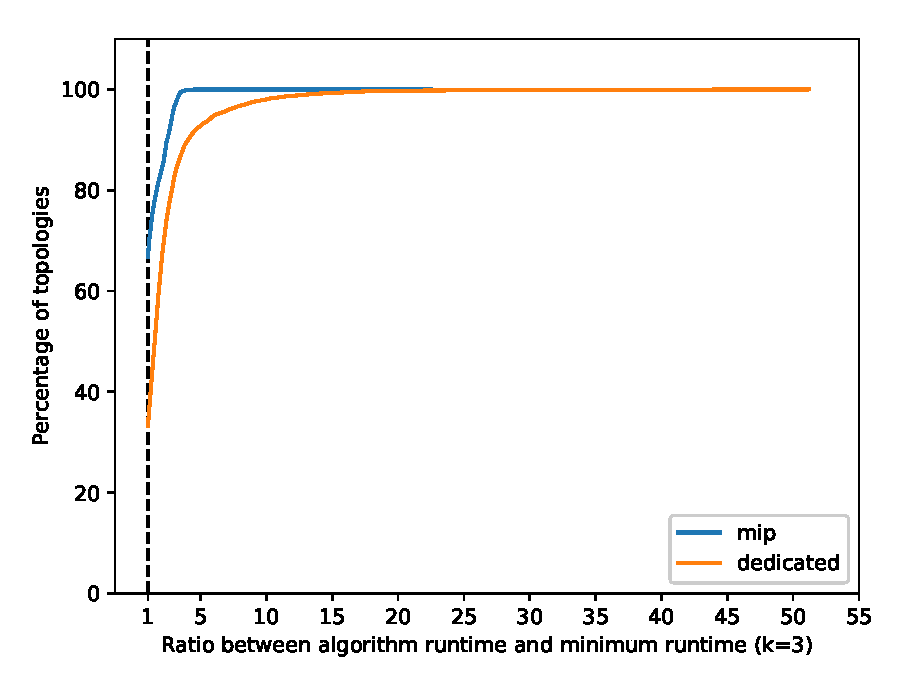
\includegraphics[width=.85\columnwidth]{./Network-lib/data/plot/2SREDP_3.eps}
\end{center}
\caption{Performance profile between the MIP model and the dedicated algorithm for $k = 3$.}
\label{fig:perf3}
\end{figure}

\begin{figure}
\begin{center}
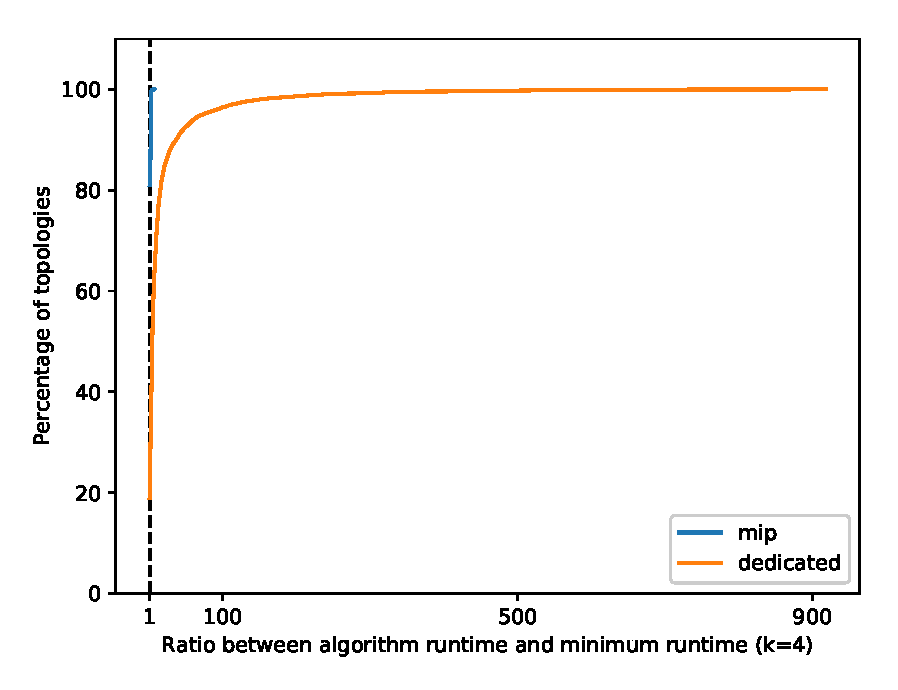
\includegraphics[width=.85\columnwidth]{./Network-lib/data/plot/2SREDP_4.eps}
\end{center}
\caption{Performance profile between the MIP model and the dedicated algorithm for $k = 4$.}
\label{fig:perf4}
\end{figure}





\section{Robustly disjoint sr-paths}
\label{section:rdp}

In this section we propose a technique to leverage segment routing to provide a failure
tolerant disjoint path service. The idea is to connect two sites via a pair of 
disjoint sr-paths like we did in the previous section and ensure these sites remain connected by two disjoint paths
even in case of a link failures. Segment routing is interesting in such
a setting because, since it is based on shortest path routing, after a set
of network links goes down, these sr-paths will automatically converge towards new paths on $G$
as the routers update theirs routing tables. 

The idea is thus to take this into account when building the sr-paths and 
make sure that the set of paths on $G$ that correspond the sr-paths are disjoint
after IGP re-convergence for any given failure. If we manage to compute such paths, then we have the guarantee
that our solution remains disjoint even in case something goes wrong.

Concretely, we will assume that a set of failure that we want to support is
given as input and we will seek pairs of paths that are tolerant to any 
failure in the given set.

\begin{definition}
Let $G$ be a network. A \emph{failure set} is a set $F = \{f_1, \ldots, f_m\}$ such that
for all $i$, $f_i \subseteq E(G)$ and $\emptyset \in F$.
\end{definition}

Requiring that the empty set belongs to the failure sets poses no practical restriction
and is there just to make the following definitions more elegant.

If we want to support single link failures we can set $F = \{ \{ e \} \mid e \in E(G) \} \cup \{ \emptyset \} = F_E(G)$.
If we know specific shared risk link groups~\cite{ghobadi-imc16,turner2010california} we can also add
them to $F$ so that our paths become failure tolerant to them.
Note that there are limits to the amount of failures that one can add to $F$. If we add too many
failure sets then we have a high chance of over constraining the problem and making it have no
admissible solution.

We model a failure of a set of edges $f \in F$ as removing those edges from the network. Therefore
it can happen that the network becomes disconnected after a failure occurs. This can lead to the fact
that the sr-paths might become undefined if they either require to route traffic between disconnected parts of the network
or they use an adjacency segment over an element of $f$. In particular, this means that we cannot use adjacency segments
over any link belonging to an edge in $F$ since such a failure would make the path unusable. As a consequence,
if $F = F_E(G)$ then we cannot use adjacency segments at all. This leads to the following definition.

%For this reason,
%we will simply ignore adjacency segments in this section and consider only paths with node segments only.

\begin{definition}
Let $G$ be a network, $\sr{p} = \langle x_1, \ldots, x_n \rangle$ a sr-path on $G$ and $F$ a failure set. We say that $\sr{p}$ is \emph{well defined
with respect to $F$} if $\sr{p}$ does not contain any adjacency segment belonging to a set $f \in F$
and for each $i = 2, \ldots, n$ and $f \in F$, $G \setminus f$ contains at least one path from $x^2_{i - 1}$ to $x^1_i$.
\end{definition}

Figure \ref{fig:welldefined} illustrates this definition. Suppose that the failure set $F$ contains a failure set $f$ whose
elements consist of all edges touching node $\node{i}$ (in both directions). Then any path using node $\node{i}$ as a segment
will not be well defined with respect to $F$. For instance, $\sr{p} = \langle \node{a}, \node{g}, \node{i}, \node{h} \rangle$
will fail to forward packets from $\node{g}$ to $\node{i}$ if failure $f$ occurs.
This example also illustrates another important aspect of robustly disjoint paths. Imagine that we want to consider node failures
and also have disjoint sr-paths that are tolerant to node failures. We can model a node failure with a failure set $f$ consisting
of all edges incident to that node (in both directions). However, this will imply that that node becomes a forbidden node segment for
any sr-path in the solution. A corollary of this is that it is impossible to have robustly disjoint paths that are tolerant to the failure of
\emph{any} node since this would prevent any sr-path to contain segments altogether.

\begin{figure}
\begin{center}
\begin{tikzpicture}
\def\x{0}
\def\y{0}

\node[scale=0.15] (a) at (0.5 + \x,  0.5 + \y) {\router{a}{marked}};
\node[scale=0.15] (b) at (0.5 + \x, -1.0 + \y) {\router{b}{router}};
\node[scale=0.15] (c) at (2.5 + \x,  0.0 + \y) {\router{c}{router}};
\node[scale=0.15] (d) at (4.5 + \x,  0.0 + \y) {\router{d}{router}};
\node[scale=0.15] (e) at (4.0 + \x, -2.0 + \y) {\router{e}{router}};
\node[scale=0.15] (g) at (6.0 + \x,  0.5 + \y) {\router{g}{marked}};
\node[scale=0.15] (i) at (8.0 + \x,  0.0 + \y) {\router{i}{marked}};
\node[scale=0.15] (h) at (7.0 + \x, -1.5 + \y) {\router{h}{marked}};
\node[scale=0.15] (f) at (4.0 + \x, -3.5 + \y) {\router{f}{router}};
\node[scale=0.15] (j) at (8.0 + \x, -2.5 + \y) {\router{j}{router}};
\draw[line width=2] (a) edge[above, sloped] node[black] {} (b);
\draw[line width=2]  (a) edge[above, sloped] node[black] {} (c);

\draw[line width=2] (b) edge[above, sloped] node[black] {} (c);
\draw[line width=2] (b) edge[above, sloped] node[black] {} (e);
\draw[line width=2] (b) edge[above, sloped] node[black] {} (f);
\draw[line width=2]  (c) edge[above, sloped] node[black] {} (d);
\draw[line width=2]  (d) edge[above, sloped] node[black] {} (e);
\draw[line width=2]  (d) edge[above, sloped] node[black] {} (g);
\draw[line width=2] (e) edge[above, sloped] node[black] {} (c);
\draw[line width=2] (e) edge[above, sloped] node[black] {} (f);
\draw[line width=2] (f) edge[above, sloped] node[black] {} (j);
\draw[line width=2] (f) edge[above, sloped] node[black] {} (h);
\draw[line width=2, red] (g) edge[above, sloped] node[black] {} (i);
\draw[line width=2]  (g) edge[above, sloped] node[black] {} (h);
\draw[line width=2] (h) edge[above, sloped] node[black] {} (j);
\draw[line width=2, red] (i) edge[above, sloped] node[black] {} (h);
\draw[line width=2]  (e) edge[above, sloped] node[black] {} (h);

\draw[line width=3, darkgreen]  (a) edge[above, bend left=15, sloped, ->] node[black] {} (c);
\draw[line width=3, darkgreen]  (c) edge[above, bend left=15, sloped, ->] node[black] {} (d);
\draw[line width=3, darkgreen]  (d) edge[above, bend left=15, sloped, ->] node[black] {} (g);
\draw[line width=3, darkgreen]  (g) edge[above, bend left=15, sloped, ->] node[black] {} (i);
\draw[line width=3, darkgreen]  (i) edge[above, bend left=15, sloped, ->] node[black] {} (h);

\node[draw, fill=green!50!white, above = 0.1cm of a] (y1) {\small $x_1$};
\node[draw, fill=green!50!white, above = 0.1cm of g] (y2) {\small $x_2$};
\node[draw, fill=green!50!white, above = 0.1cm of i] (y3) {\small $x_3$};
\node[draw, fill=green!50!white, right = 0.1cm of h] (y3) {\small $x_4$};

\end{tikzpicture}
\end{center}
\caption{The sr-path $\langle \node{a}, \node{g}, \node{i}, \node{h} \rangle$ is not well defined if edges 
$\edge{g}{i}$, $\edge{i}{g}$, $\edge{i}{h}$, $\edge{h}{i}$ are in $F$.}
\label{fig:welldefined}
\end{figure}


We can now define the robustly disjoint paths (RDPs).

\begin{definition}
Let $G$ be a network, $\sr{p}_1$, $\sr{p}_2$ be two sr-paths and $F$ a failure set. We say that
$\sr{p}_1$ and $\sr{p}_2$ are \emph{robustly disjoint} if they are disjoint and well defined
on $G \setminus f$ for every $f \in F$.
\end{definition}

You can see that this definition also ensures that robuslty disjoint paths are 
disjoint to begin with since we assume that $\emptyset \in F$.

\begin{problem}{Robustly disjoint sr-path problem}
\label{prob:rdp}
\textbf{Input:} A network $G$, a failure set $F$, $s_1, s_2, t_1, t_2 \in V(G)$ and $k \in \mathbb{N}$.

\textbf{Output:} Two robustly disjoint sr-paths $\sr{p}_1 \in \Pk(s_1, t_1)$, $\sr{p}_2 \in \Pk(s_2, t_2)$ with respect to $F$.
\end{problem}

Since Problem \ref{prob:disjointsrp} is \NPhard, this problem must also be since we get the same problem
by setting $F = \{ \emptyset \}$.

It is not hard to adapt the disjoint sr-path MIP model proposed in the previous section 
to the case of robustly disjoint paths as well as our dedicated algorithm as we will show in the
remainder of this section.

\subsection{Adapting $\sredp$ to RDPs}

Adapting model $\sredp(G, s_1, s_2, t_1, t_2)$ to support robustly disjoint paths
is very simple. The only thing that we need to change are the disjointness constraints
so that they take the failures into account.

Recall that we ensure disjointness by requiting that if $e \in E(\sp(u, v))$ then
at most one of $x^1_{uv}, x^2_{uv}$ is set to $1$. To ensure that the sr-paths 
are robuslty disjoint we need to ensure that if
$$
e \in \bigcup_{f \in F} E(\sp(G \setminus f, u, v))
$$
then at most one of $x^1_{uv}, x^2_{uv}$ is equal to $1$.

For this we define a new indicating function $I_F$ such that $I_F(u, v, e) = 1$
if and only if $e$ belongs to the shortest paths between $u$ and $v$ 
on $G \setminus f$ for some $f \in F$. The robuslty disjoint path model
are obtained by replacing $I$ by $I_F$.

The cost of this adaptation is of course that pre-computing these $I_F$ functions takes more time,
specially if $F$ is very large. However, this is only needed to be done once. We can build the model
once and only adapt it for the specific sources and destinations before each computation. Using the MIP model
is also more flexible and can easily be extended to compute more than two paths. 

\subsection{Adapting the dedicated algorithm to RDPs}

Algorithms \ref{algo:disjoint_srp} and \ref{algo:disjoint_srp_dfs} are also easily adaptable
to the case of robuslty disjoint paths but this results in a very inefficient algorithm.
The problem is that checking whether the paths are disjoint after any failure requires 
$|F|$ bit set comparisons meaning that each step of the algorithm is $|F|$ times slower.
For completeness we will describe the needed modifications on the algorithms.

To ensure that the sr-paths computed by the algorithm are well defined, 
we need to prevent the algorithm from using consecutive node segments $u, v$ such that 
there is no path from $u$ to $v$ in $G \setminus f$. Also, we need to forbid any adjacency 
segment over an edge belonging to some $f \in F$. Both these steps can be achieved by
pre-computing the pairs of nodes that cannot appear as consecutive segments and 
preventing to use adjacency segments on the set $\{ e \in f \mid f \in F\}$. Contrary to the
next modification, this only slows down the preprocessing step of the algorithm, not the
algorithm itself.

What really slows down the algorithm is that we need to also ensure disjointness after any failure $f \in F$ occurs.
To avoid having to make $|F|$ shortest path computations we can pre-compute
$\sp(G \setminus f, u, v)$ for all $f \in F$ and $u, v \in V(G)$. Now instead of checking
for intersection between $E(\sr{p}_1)$ and $E(\sr{p}_2)$ we need to check 
for intersection for every $f \in F$. This is the reason why the algorithm is 
not usable in practice for generic failures unless $F$ is quite small. Note that this is not the case for the
MIP adaptation above, we need more time to build the model because of the
indicating function $I_F$ takes longer to compute but that is not really a problem
since it needs to be done only once for any given topology. We will see however
in the next sections that if $F = F_E$ (single-link failures) then we can
still obtain a fast algorithm.

\subsection{The case of single-link failures}

Recall from the above discussion that the bottleneck in adapting 
Algorithms \ref{algo:disjoint_srp} and \ref{algo:disjoint_srp_dfs} to the case of 
robustly disjoint paths is checking whether the paths are disjoint for every failure.
We are going to see how we can check this efficiently when the set of failures is the 
set of edges thus showing that computing robustly disjoint paths that are tolerant to 
single-link failures can be done efficiently in practice.

The idea is that we will aggregate all the edges in $\sp(G \setminus f, u, v)$ for all $f \in F$
into a single set that we call \emph{failure set}. And then we show that checking for intersection
between the failures sets is enough to ensure robustness when $F = F_E$.

\begin{definition}
Let $G$ be a network and $\sr{p} = \langle x_1, \ldots, x_n \rangle$ a sr-path on $G$. We define the \emph{failure set of $\sr{p}$}
as
$$
\fail(\sr{p}) = \bigcup_{f \in F_G} E(G \setminus f, \sr{p})
$$
%$$
%\fail(\sr{p}) = \left( \bigcup_{e \in E(G)} \bigcup_{i = 2}^n E(\sp(G \setminus e, x^2_{i - 1}, x^1_i)) \right) \cup \bigcup_{i : x_i \in E(G)} x_i
%$$
\end{definition}

The next result is a very simple lemma that states that a failure on an edge that is not used by a sr-path does not affect it. This is quite an
obvious result but it is important for the theorem that follows.

\begin{lemma}
\label{lemma:outside-edge}
Let $G$ be a network and $\sr{p}$ a sr-path on $G$. If $e \in E(G) \setminus E(\sr{p})$ then $E(G \setminus e, \sr{p}) = E(G, \sr{p})$.
\end{lemma}

\begin{proof}
Let $e \in E(G) \setminus E(\sr{p})$ and write $\sr{p} = \langle x_1, \ldots, x_n \rangle$. Since $e \notin E(\sr{p})$ we have 
that for each $i \in \{2, \ldots, n\}$, $\sp(G, x^2_{i - 1}, x^1_{i}) = \sp(G \setminus e, x^2_{i - 1}, x^1_{i})$. Also, $e$ cannot be an
adjacency segment of $\sr{p}$ or else it would belong to $E(\sr{p})$. Therefore,
\begin{align*}
E(G \setminus e, \sr{p}) & = \left( \bigcup_{i = 2}^n E(\sp(G \setminus e, x^2_{i - 1}, x^1_i)) \right) \cup \bigcup_{i : x_i \in E(G) \setminus e} x_i \\
& = \left( \bigcup_{i = 2}^n E(\sp(G, x^2_{i - 1}, x^1_i)) \right) \cup \bigcup_{i : x_i \in E(G) } x_i \\
& = E(G, \sr{p}).
\end{align*}
\end{proof}

The following theorem shows how we can efficiently check disjointness conditions for every failure in the case of single-link
failures.

\begin{theorem}
\label{thm:single-link}
Let $G$ be a network and $\sr{p}_1, \sr{p}_2$ be two sr-paths on $G$. Then $\sr{p}_1, \sr{p}_2$ are robustly
disjoint with respect to $F_E$ if and only if they are well defined, $\fail(\sr{p}_1) \cap E(\sr{p}_2) = \emptyset$ and 
$E(\sr{p}_1) \cap \fail(\sr{p}_2) = \emptyset$.
\end{theorem}

\begin{proof}
$(\Rightarrow)$ Suppose that $\sr{p}_1, \sr{p}_2$ are robustly disjoint. 
Thus for each $f \in F_E$ we have $E(G \setminus f, \sr{p}_1) \cap E(G \setminus f, \sr{p}_2) = \emptyset$.
Since $\emptyset \in F_E$ we have in particular that $\sr{p}_1$ and $\sr{p}_2$ are disjoint on $G$. Suppose that $\fail(\sr{p}_1) \cap E(\sr{p}_2) \neq \emptyset$.
Then there exists $e \in E(G, \sr{p}_1)$ such that $E(G \setminus e, \sr{p}_1) \cap E(G, \sr{p}_2) \neq \emptyset$. Since the paths are disjoint, 
it cannot be the case that $e \in E(G, \sr{p}_2)$. Therefore, by Lemma \ref{lemma:outside-edge} we have that $E(G \setminus e, \sr{p}_2) = E(G, \sr{p}_2)$.
This means that $E(G \setminus e, \sr{p}_1) \cap E(G \setminus e, \sr{p}_2) = E(G \setminus e, \sr{p}_1) \cap E(G, \sr{p}_2) \neq \emptyset$ contradicting the
fact that the sr-paths are robustly disjoint. The case where $E(\sr{p}_1) \cap \fail(\sr{p}_2) \neq \emptyset$ is analogous.

$(\Leftarrow)$ Suppose that $\sr{p}_1, \sr{p}_2$ are well defined and that $\fail(\sr{p}_1) \cap E(\sr{p}_2) = \emptyset$ and 
$E(\sr{p}_1) \cap \fail(\sr{p}_2) = \emptyset$. Assume that the paths are not robustly disjoint for $F_E$. Since they are well defined, 
this means that either $E(\sr{p}_1) \cap E(\sr{p}_2) \neq \emptyset$ or
there exists $e \in E(G)$ such that $E(G \setminus e, \sr{p}_1) \cap E(G \setminus e, \sr{p}_2)$. Since $\emptyset \in F_G$ we have
that $E(\sr{p}_1) \subseteq \fail(\sr{p}_1)$ and thus $E(\sr{p}_1) \cap E(\sr{p}_2) \subseteq \fail(\sr{p}_1) \cap E(\sr{p}_2) = \emptyset$. Then, let $e$ be such that
$E(G \setminus e, \sr{p}_1) \cap E(G \setminus e, \sr{p}_2) \neq \emptyset$. Since $E(\sr{p}_1) \cap E(\sr{p}_2) = \emptyset$, $e$ cannot belong to both
$E(\sr{p}_1)$ and $E(\sr{p}_2)$. If it does not belong to $E(\sr{p}_1)$ then by Lemma \ref{lemma:outside-edge} we have 
$E(G \setminus E, \sr{p}_1) = E(\sr{p}_1)$ so 
$\emptyset \neq E(G \setminus e, \sr{p}_1) \cap E(G \setminus e, \sr{p}_2) = E(\sr{p}_1) \cap E(G \setminus e, \sr{p}_2) \subseteq E(\sr{p}_1) \cap \fail(\sr{p}_2) = \emptyset$
which is a contradiction. The other case is analogous and also leads to a contradiction. It follows that the paths are robustly disjoint.
\end{proof}

Using Theorem \ref{thm:single-link} we can transfer the time it takes for checking whether paths remain disjoint to
a pre-computation step where we compute the failure sets defined above for each two nodes $u, v \in V(G)$. Using these 
we can incrementally build the failure sets as we build $\sr{p}_1$ by noting that if $\sr{p}_1 = \langle x_1, \ldots, x_n \rangle$ then
$$
\fail(\sr{p}) = \left( \bigcup_{i = 2}^n \fail(\langle x^2_{i - 1}, x^1_i \rangle) \right) \cup \bigcup_{i : x_i \in E(G)} x_i.
$$

Therefore, whenever we extend $\sr{p}_1 = \langle x_1, \ldots, x_n \rangle$ with a segment $x$, we simply need to make 
the union of the current failure set with the precomputed failure set $\fail \langle x^2_n, x \rangle$ and $x_i$ if $x_i$
is an adjacency segment. Again, because of the use of bitset, this is a lightweight operation.

These only need to be pre-computed once for each given topology. We propose an efficient algorithm that is able to
compute them in under a minute even on the largest topologies. Thus it is 
reasonable to recompute them whenever the topology changes as these do not happen every minute.

% We already briefly mentioned above where the changes need to be applied in the algorithm for implementing robustness. For completeness we 
% will explicitly show the changes for the case of single-link failures.
% 
% \todo{complete this}

\subsubsection{Pre-computing the failure sets}

As we showed above, the failure sets for single-link failures are composed of the failure sets of the sr-path $\langle x, y \rangle$.
We are now going to describe how we can compute these efficiently. If we followed the definition we would loop over all pairs $x, y \in V(G)$ and
edges $e \in E(G)$ and for each edge we would compute the shortest path subnetwork from $x$ to $y$ on $G \setminus e$. 
However this is very costly. Instead, we can take advantage of Lemma \ref{lemma:forwdp}. For each fixed $x$ and $e \in E(G)$ we will compute the
shortest path subnetwork rooted at $x$. Then we compute a topological order of it and use Equation (\ref{eq:forwdp}) to compute
$E(\sp(G \setminus e, x, y))$.

We also add two ideas to accelerate the algorithm. The first is based on Lemma \ref{lemma:outside-edge}. It simply consists of ignoring
sets $e \notin E(\sp(x, y))$ since these will not add any new edges to $\fail \langle x, y \rangle$. The second idea is that we can ignore edges that
belong to an ECMP component between $x$ and $y$ since removing them will also not contribute to any new shortest paths because there will
always be at least one of the previous shortest paths that remains after the removal of $e$.
A formalization of this is provided as Algorithm \ref{algo:prefail}.

\begin{algorithm}[t]
\small
\caption{$\textsf{precompute-failEdges}\left( G, \sp, fwe \right)$}
\begin{algorithmic}[1]
\FOR{$u, v \in V(G)$}
  \STATE $\fail(u, v) \gets fwe(u, v)$
\ENDFOR
\FOR{$u \in V(G)$}
  \cmtline{optim 1: only consider edges in $\sp(u)$ as the others have no effect}
  \FOR{$f \in E(\sp(u))$}
    \cmtline{optim 2: check degree to consider only edges not in ECMP components}
    \IF{$\delta^-(\sp(u), f^2) \leq 1$}
      \STATE $\sp(f, u) \gets \textsf{dikstra-dag}(G \setminus f, u)$
      \STATE $order \gets \textsf{toposort}(\sp(u))$
      \FOR{$v \in order$}
	\FOR{$e \in \ine(\sp(u), v)$}
	  \STATE $\fail(u, v) \gets \fail(u, e^1) \cup \{ e \}$
	\ENDFOR
      \ENDFOR
    \ENDIF
  \ENDFOR
\ENDFOR
\RETURN $\fail$
\end{algorithmic}
\label{algo:prefail}
\end{algorithm}

\subsection{Evaluation of RDPs}

\subsubsection{Evaluating effective robustness of RDP}

Using the above concepts we can compute pairs of sr-paths that are robustly disjoint to single-link failures.
This is what our theoretical results guarantee. However, it could very well be the case that our paths are actually
robust to a lot more failures. We performed an experiment to evaluate this. For $s = 1, \ldots, 6$, we
generated $100$ sets of $s$ simultaneous link failures. We consider two kinds of failures sets: selecting random
links from the whole topology and selecting random links that are used by the sr-paths.
These second failure sets are generated so that each of them
affects the paths. So for instance, on a failure set with $s = 3$ we select the first link to be one of
the links used by our pair of sr-paths. Then compute the paths resulting from that failure and select the second
link randomly among the resulting links. For the third link we do the same. This ensures that we are not biasing our
results by the fact that with high probability selecting a random link will not even affect the paths. In general,
the $n$-th failure is selected from the paths resulting from the previous $n - 1$ failures. For each failure set
we evaluate the end state of the paths and consider the following four states:

\begin{enumerate}[i)]
 \item \emph{disjoint}: the paths remain disjoint after the failures;
 \item \emph{not disjoint}: both paths remain defined but not disjoint;
 \item \emph{one disconnected}: one path becomes disconnected;
 \item \emph{both disconnected}: both paths became disconnected.
\end{enumerate}

Figures \ref{fig:failure_sets_worst} and \ref{fig:failure_sets_best}
show the results on the topologies in our dataset for which we respectively get
the best and worst results in terms of robustness to additional failures (all
the other topologies are included between those extremes).
For the best case, shown in Figure \ref{fig:failure_sets_worst} paths remain disjoint with no configuration change in almost all the
simulations, including those with 6 simultaneous link failures, and
source-destination tuples are disconnected very rarely (0.01\% of the time for 6
link failures).
For the wost case, shown in Figure \ref{fig:failure_sets_best}, results remain very good for random failures, but are significantly
worse for the worst-case failures. Still, connectivity is often kept between
source-destination tuples, e.g., for more than 80\% (about 70\%, respectively)
of the experiments in the presence of 5 (6, respectively) successive on-path
failures.

\begin{figure}
\begin{center}
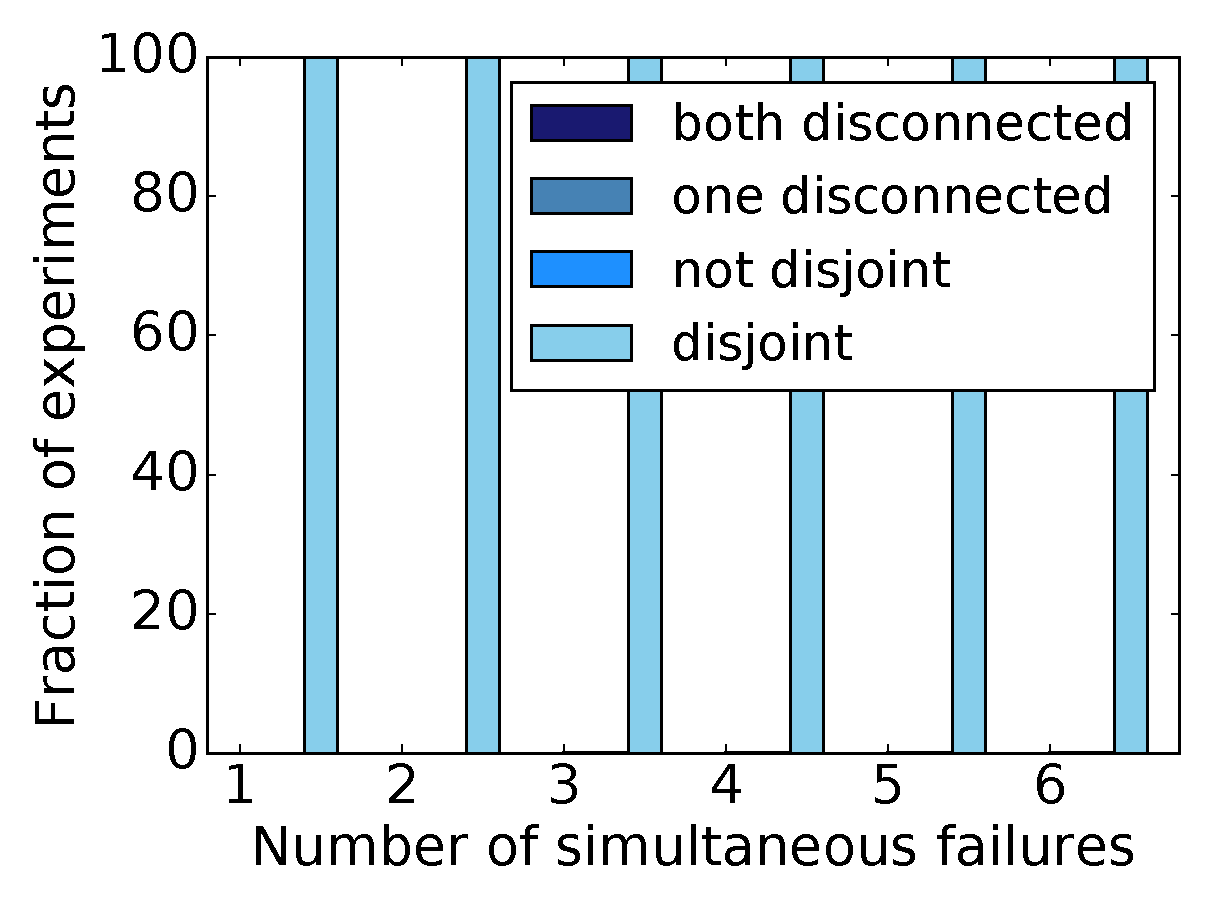
\includegraphics[width=0.45 \columnwidth]{figures/real1_random.eps}
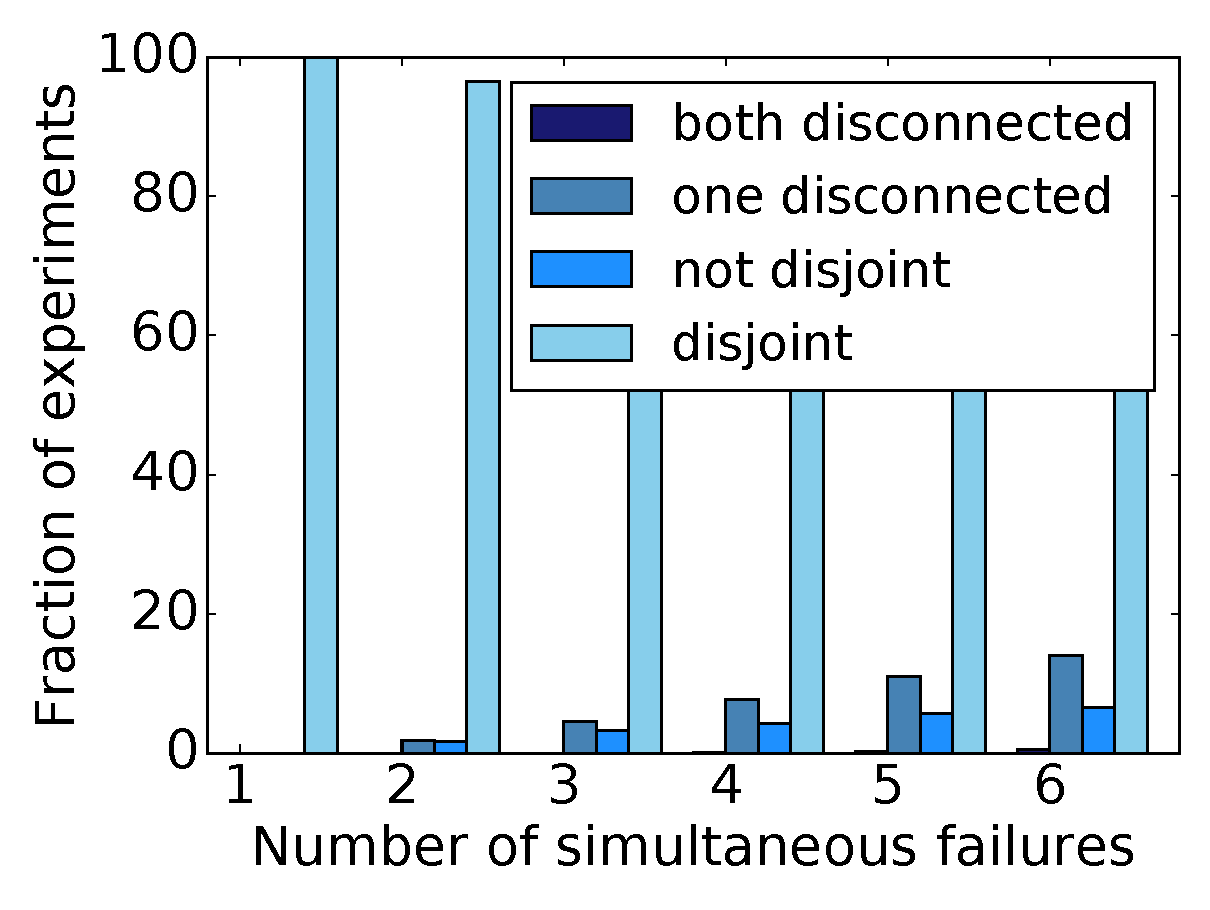
\includegraphics[width=0.45 \columnwidth]{figures/real1_worst.eps}
\end{center}
\caption{Random failures and path link failures over the worst case topoology.}
\label{fig:failure_sets_worst}
\end{figure}

\begin{figure}
\begin{center}
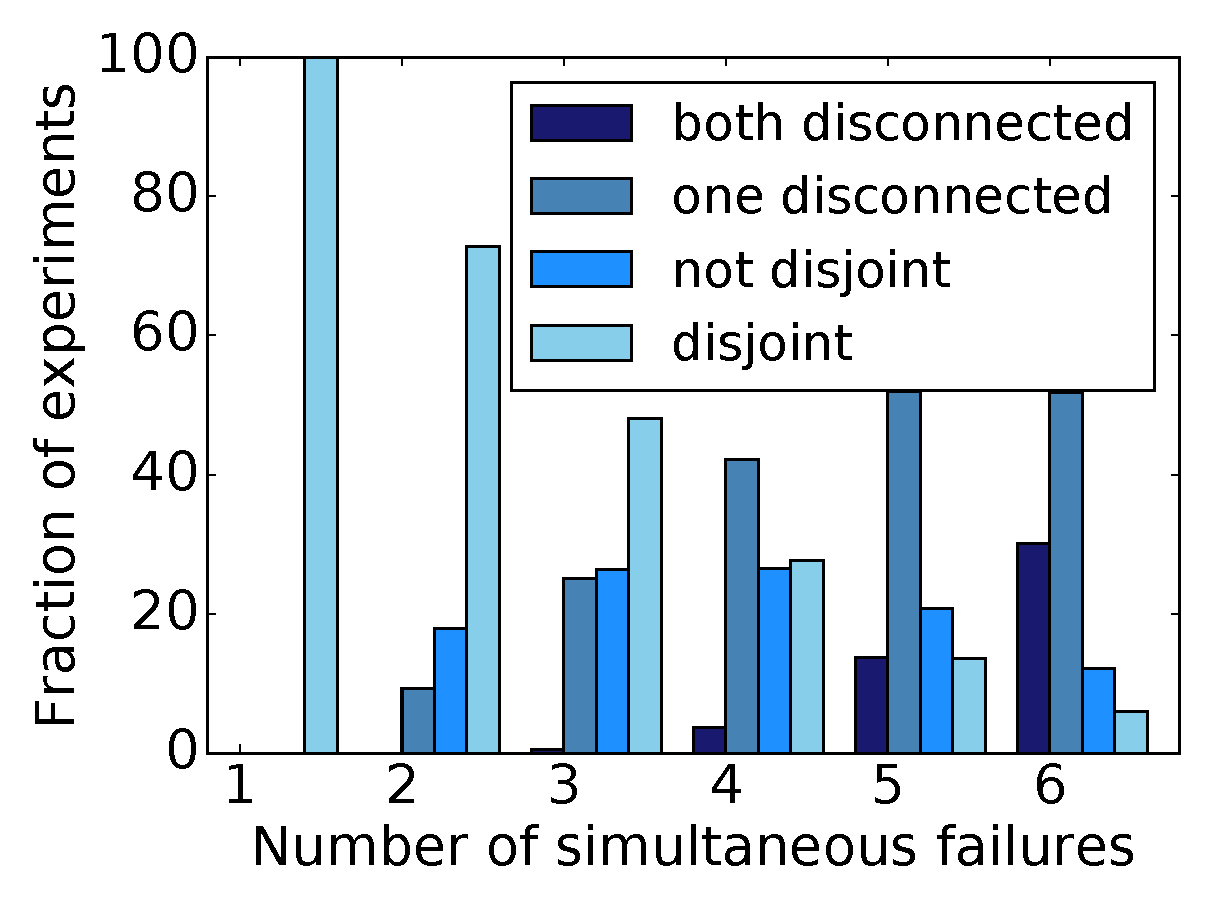
\includegraphics[width=0.45 \columnwidth]{figures/DialtelecomCz_worst.eps}
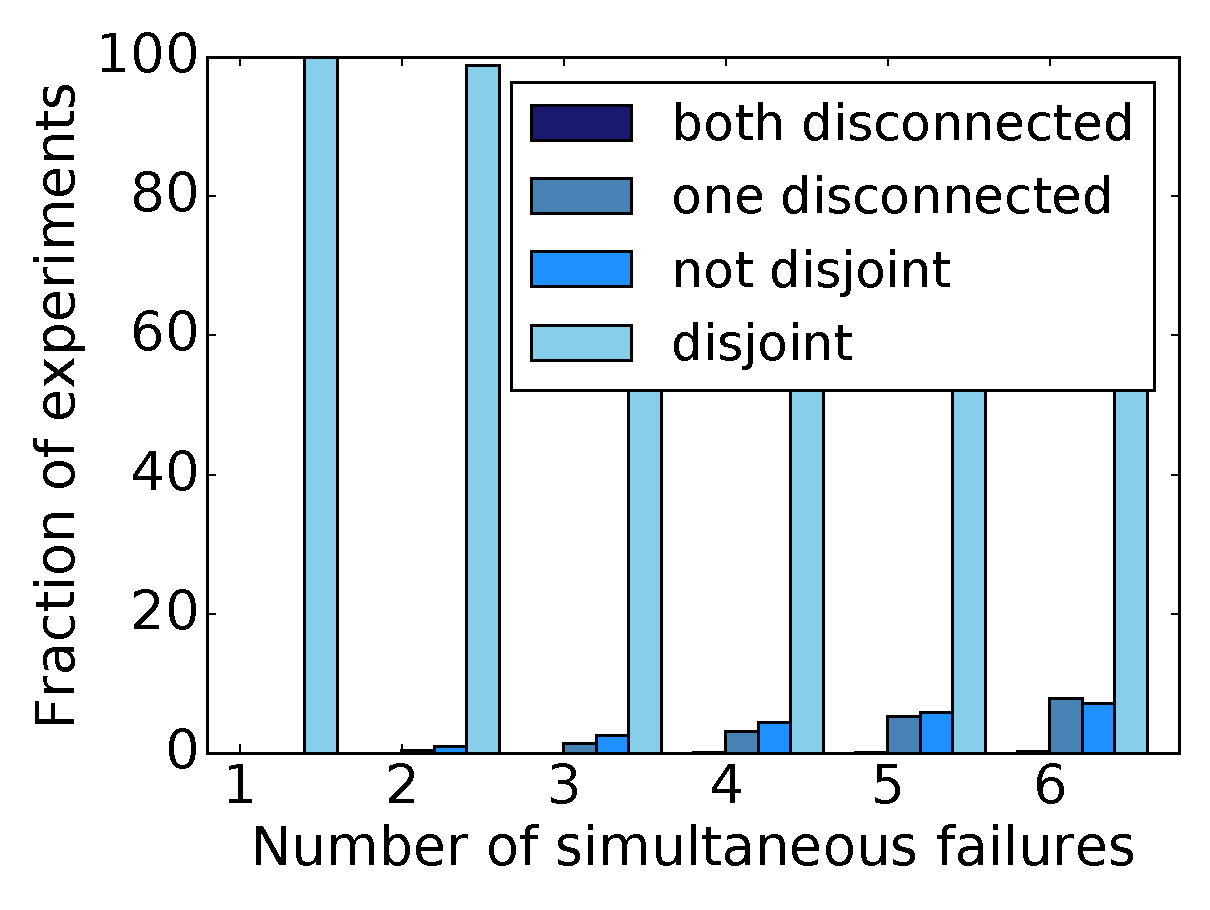
\includegraphics[width=0.45 \columnwidth]{figures/DialtelecomCz_random.eps}
\end{center}
\caption{Random failures and path link failures over the best case topology.}
\label{fig:failure_sets_best}
\end{figure}

We wondered whether we could evaluate the robustness of a pair of sr-paths algorithmically rather than 
having to perform such an experiment. The following theorem shows that it is $\NPhard$ to compute the minimum number of failures
that a pair of sr-paths can withstand until they cease to be disjoint.

\begin{problem}{Minimum cardinality failure}
\label{prob:eff-rob} 
\textbf{Input:} A network $G$ and two sr-paths $\sr{p}_1$ and $\sr{p}_2$.

\textbf{Output:} The cardinality of a minimal set of links $f \subseteq E(G)$ such that
$\sr{p}_1$ and $\sr{p}_2$ are not disjoint on $G \setminus f$.
\end{problem}

\begin{theorem}
Problem \ref{prob:eff-rob} is \NPhard. 
\end{theorem}

The following proof resulted from discussions with a student of mine, Simon Tihon, while I was coaching 
him for algorithmic programming contents.

\begin{proof}
To prove that this problem is $\NPhard$ it is enough to prove that the problem is $\NPhard$ for sr-paths of the form
$\sr{p}_1 = \langle s_1, t_1 \rangle$ and $\sr{p}_2 = \langle s_2, t_2 \rangle$. This amounts to,
given four nodes $s_1, s_2, t_1$ and $t_2$, find the minimum numbers of edges that we need to remove so that
the shortest paths from $s_1$ to $t_1$ intersect the shortest paths from $s_2$ to $t_2$.

It is known that the problem of finding the minimum number of edges that need to be removed so that the shortest path
between two given nodes becomes strictly larger than a given value $d$ is $\NPhard$ \cite{Golovach2011PathsOB}. Let $G, s, t, d$ be an instance
of this problem and assume that we can solve our problem
is polynomial time. We can assume that the shortest path between $s$ and $t$ has cost lower than or equal to $d$ or otherwise the problem is trivial.
e build an instance of Problem \ref{prob:eff-rob} by setting $s_2 = s, t_2 = t$ and adding two
nodes $s_1, t_1$. We connect $s_1$ to $s_2$ with an link of weight $d$ and $t_1$ to $t_2$ with a link of weight
$0$. Nodes $s_1$ and $t_1$ are connected with $K + 1$ parallel edges of weight $0$ where $K$ is the value of the
minimum cut between $s$ and $t$ on $G$. Figure \ref{fig:reduction} illustrates this construction.

\begin{figure}[H]
\begin{center}
\begin{tikzpicture}
\draw[ultra thick, dashed, fill=gray!50!white] (3, -1.5) ellipse (1 and 2.5);

% \node[draw, circle, fill=lightgray] (s1) at (0, 0) {$s_1$};
% \node[draw, circle, fill=lightgray] (s2) at (3, 0) {$s_2$};
% \node[draw, circle, fill=lightgray] (t1) at (0, -3) {$t_1$};
% \node[draw, circle, fill=lightgray] (t2) at (3, -3) {$t_2$};

\node[scale=0.15] (s1) at (0,  0) {\router{$s_1$}{marked}};
\node[scale=0.15] (s2) at (3,  0) {\router{$s_2$}{marked}};
\node[scale=0.15] (t1) at (0,  -3) {\router{$t_1$}{marked}};
\node[scale=0.15] (t2) at (3,  -3) {\router{$t_2$}{marked}};


\draw (s1) edge[ultra thick, bend left = 50, sloped, above] node {$0$} (t1);
\draw (s1) edge[ultra thick, bend left = 20, sloped, above] node {$0$} (t1);
\draw (s1) edge[ultra thick, bend right = 50, sloped, above] node {$0$} (t1);
\draw (s1) edge[ultra thick, bend right = 20, sloped, above] node {$0$} (t1);

\node at (0, -1.5) {$\ldots$};

\node at (-2, -1) {$K + 1$ edges};


\draw (s1) edge[ultra thick, above] node {$d$} (s2);
\draw (t1) edge[ultra thick, above] node {$0$} (t2);


\node at (3, -1.5) {$G$};

\end{tikzpicture}
\end{center}
\caption{Construction used in the problem reduction.}
\label{fig:reduction}
\end{figure}

The shortest paths between $s_1$ and $t_1$ consists of the parallel links between them
whereas the shortest paths between $s_2 = s$ and $t_2 = t$ lie on $G$ since we assumed that the shortest
path from $s$ to $t$ has a cost lower than $d$. Note that the path visiting nodes $(s_2, s_1, t_1, t_2)$ has cost
$d$. Therefore, the shortest path from $s_2$ to $t_2$ will intersect the shortest paths from $s_1$ to $t_1$ if and only
if the shortest path from $s_1$ to $t_1$ on $G$ costs more than $d$.
Clearly, the minimum number of edges that we need to remove
so that the cost of the shortest path from $s$ to $t$ becomes at least $d$ is at most $K$ since $K$
is the value of a minimum cut (and thus a solution). Thus after removing this set the path are still well defined
since we have $K + 1$ parallel edges.
\end{proof}

\subsubsection{Evaluating existence and quality of RDPs}

In this section we will use the word detour to refer to an intermediate 
node that is in the segment stack. More concretely, for a sr-path of the form
$\langle x_1, x_2, \ldots, x_{n - 1}, x_n \rangle$, the detours are the nodes
$x_2, \ldots, x_{n - 1}$. Clearly a sr-path with $r$ detours has segment cost
$r + 2$.

We focus on reasonably well-connected \textit{source-destination
tuples}. For each topology, we randomly select 100 tuples $(s_1, s_2, t_1, t_2)$
of two sources $s_1,s_2$ and two destinations $t_1,t_2$, such that $s_1$ and
$s_2$ have a path to $t_1$ and $t_2$ even when any edge is removed. Since we try to
compute robustly disjoint paths from $s_1$ to $t_1$ and from $s_2$ to $t_2$,
it would indeed make little sense to consider source-destination pairs that are
disconnected by a single failure -- it is obvious that a service provider cannot offer
a robust connectivity service between routers that are poorly connected.
We repeat each experiment allowing between 1 and 3 detours ($k = 3, 4, 5$). We stop
at 3.

Table \ref{tab:rdp_existence} shows the percentage of these tuples for which robustly
disjoint paths exist. Sometimes, only selecting the right IGP paths is sufficient
for a given tuple. However, since IGP costs are shared across all
paths, they rarely can be used for more than one source-destination
tuple, preventing operators to configure robustly disjoint paths for
multiple customers or between different sites of the same customer.
Adding one detour by specifying an intermediate node with SR
allows paths for different tuples to be independent from each other,
solving the above issue. It also drastically increases the percentage
of tuples with at least one pair of robustly disjoint paths to 71%-100%
across all the topologies, and to 97% or more for all topologies but
two. Allowing more detours provides only slightly more flexibility
in our experiments.

\begin{figure}
\begin{center}
\begin{tabular}{ l | c c c c }
  \toprule
  & \multicolumn{3}{c}{Number of detours} \\
  Topology & 0 det & 1 det & 2 det & 3 det \\
  \midrule
  Real ISP 1 & 83\% & 100\% & 100\% & 100\% \\
  Real ISP 2 & 89\% & 100\% & 100\% & 100\% \\
  Real ISP 3 & 73\% & 100\% & 100\% & 100\% \\
  \midrule
  AS 1221 & 82\% & 98\% & 100\% & 100\% \\
  AS 1239 & 90\% & 100\% & 100\% & 100\% \\
  AS 1755 & 52\% & 98\% & 100\% & 100\% \\
  AS 3257 & 76\% & 100\% & 100\% & 100\% \\
  AS 3967 & 71\% & 99\% & 100\% & 100\% \\
  AS 6461 & 75\% & 100\% & 100\% & 100\% \\
  \midrule
  ITZ Cogentco & 78\% & 97\% & 100\% & 100\% \\ 
  ITZ Colt & 58\% & 71\% & 73\% & 73\% \\
  ITZ Deltacom & 74\% & 99\% & 99\% & 100\% \\
  ITZ Dia & 54\% & 77\% & 79\% & 79\% \\
  ITZ GtsCe & 78\% & 98\% & 100\% & 100\% \\
  ITZ Interoute & 81\% & 99\% & 100\% & 100\% \\
  ITZ Ion & 64\% & 100\% & 100\% & 100\% \\
  ITZ Tata & 86\% & 100\% & 100\% & 100\% \\
  ITZ UsCarrier & 72\% & 83\% & 85\% & 85\% \\
  \bottomrule
\end{tabular}
\end{center}
\caption{Percentage of tuples for which RDPs exist.}
\label{tab:rdp_existence}
\end{figure}

Our algorithms are designed to find sr-paths that are both
robustly disjoint and have minimal worst-path delay. As 
table \ref{tab:rdp_lat} shows, the robustly disjoint paths computed by our
algorithms have a worst-path delay which is always better than
the worst latency across the original IGP shortest paths. We are
up to 15\% more efficient, on average. Once again, more detours
enable to decrease the latency of the computed paths across all the
topologies, but just negligibly in most cases.

\begin{figure}
\begin{center}
\begin{tabular}{ l | c c c }
  \toprule
  & \multicolumn{3}{c}{Number of detours} \\
  Topology &  1 det & 2 det & 3 det \\
  \midrule
  Real ISP 1 & 0.97 & 0.97 & 0.97 \\
  Real ISP 2 & 0.98 & 0.98 & 0.98  \\
  Real ISP 3 & 0.97 & 0.96 & 0.96  \\
  \midrule
  AS 1221 & 0.99 & 0.99 & 0.99 \\
  AS 1239 & 0.97 & 0.97 & 0.97  \\
  AS 1755 & 0.90 & 0.89 & 0.88  \\
  AS 3257 & 0.91 & 0.89 & 0.88\\
  AS 3967 & 0.97 & 0.97 & 0.97  \\
  AS 6461 & 0.97 & 0.97 & 0.97  \\
  \midrule
  ITZ Cogentco & 0.85 & 0.84 & 0.84  \\ 
  ITZ Colt & 0.88 & 0.87 & 0.86  \\
  ITZ Deltacom & 0.91 & 0.90 & 0.90  \\
  ITZ Dia & 0.96 & 0.98 & 0.98  \\
  ITZ GtsCe & 0.78 & 0.77 & 0.75 \\
  ITZ Interoute & 0.93 & 0.91 & 0.90   \\
  ITZ Ion & 0.95 & 0.94 & 0.94  \\
  ITZ Tata & 0.90 & 0.89 & 0.89  \\
  ITZ UsCarrier & 0.92 & 0.92 & 0.92   \\
  \bottomrule
\end{tabular}
\end{center}
\caption{Average ratio between the RPD latency and the nominal latency.}
\label{tab:rdp_lat}
\end{figure}

To assess the benefits of robustly disjoint paths in a real-life scenario, 
we also analyse a 1-week trace of all the link-state IGP packets
exchanged by a router in Real ISP2. Based on this trace, we identified 
that a total of 5\% of the links failed during this period. Some
links experienced flapping, confirming observations of previous
studies [28, 45]. For example, one of the links failed more than 30
times during the analysed week. We select 100 source-destination
pairs in this network, and compute the corresponding robustly
disjoint paths for F = E (all single-link failures). We then replayed
all the failures that happened during the entire week. The 
source-destination pairs always have disjoint paths in our simulation, at
any moment during the week, even when multiple edges failed
simultaneously. This experiment provides a strong indication that
the paths computed by our algorithms are robust to real failures,
for a long time, in an operational network, without the need for
any configuration adjustment.




\chapter{Conclusion}

In this thesis we proposed a first mathematical formalization of segment routing. So far, segment routing had been used
to solve some networking problems such as traffic engineering but the further that these results would go in terms of 
formalization was showing how to model segment routing in terms of linear constraints.

We go a step further and show interesting results about the structure of these segment routing paths. We showed that these
results have practical applications by exploiting them to solve several algorithmic problems related to segment routing. \\

The most important results were:

\begin{itemize}

 \item Minimal segmentations can be computed in polynomial time. This result opens the door to solving segment routing problems
 by ignoring segment routing constraints and solving the problem as a graph problem and only segmenting the resulting paths
 in the end. This is, of course, not always applicable in practice as solving problem in this way yields results that are
 sub-optimal in terms of the number of segments used in the final solution. Nevertheless, as the routers' capacity to support segments
 increases, we believe that this will become the standard approach.
 
 \item We can always connect two connected routers with a acyclic sr-path. This result can be leveraged to prune cyclic solutions on
 problems where we can prove that a cyclic sr-path will always be sub-optimal.
 
 \item In some applications, such as network monitoring, we need to be know exactly which network links are used to forward traffic. We
 defined a notion of determinism for sr-paths that expresses this requirement. We provided bound on the minimum segment cost to connect
 two nodes of any given network with deterministic sr-paths.
 
 \item Computing a cycle cover of a graph that uses a minimal amount of segments to 
 represent the cycles can be achieve in polynomial time.
 
 \item Computing minimum cost sr-paths can be done in polynomial time. The algorithm can be leveraged to compute
 minimum latency sr-paths and maximum capacity sr-paths.
 
\end{itemize}

Apart from this more theoretical aspect, we have also showed how to exploit segment routing on several real world applications.

\begin{itemize}
 \item We showed that we can leverage segmenting for network monitoring of single link failures. We proposed an algorithm that yields a
 solution with minimal segment cost. We also extended that solution using column generation in order to try to reduce the number 
 probes that are necessary for monitoring.
 
 \item We propose an alternative solution for the traffic engineering problem with segment routing based on column generation. Our 
 solution provided near optimal solutions that run faster than previous linear programming models. It also provides a lower bound so we can
 evaluate how good the solution is.
 
 \item Robust and low latency connections are important for applications that require low latency. We showed how we can compute and
 implement disjoint path using segment routing. We also improved on this solution by exploiting properties of segment routing paths 
 for providing failure tolerance guarantees to our solution.
\end{itemize}

While writing this thesis we also left some open problems which show that there is still a lot to be done when is comes to
segment routing. Our results show that the deployment of segment routing can lead to improved communications with low 
overhead. 

\begin{itemize}
 \item We showed that we can compute a sr-cycle cover of a network in polynomial time but our complexity is still quite high.
 How fast can we solve this problem?
 
 \item Suppose that we know a set of paths that we want to implement on a network. How to select IGP weights so that the maximum
 cost of the minimal segmentation of those paths is as small as possible?
 
 \item How can we find IGP weights that are ECMP-free and complete and no weight is above a given constant? Could these weights
 we a solution to the previous problem?
 
 \item We also proposed several column generation models but we did not solve them to optimality by doing, for instance,
 a branch-and-price. How efficiently can this be achieved?
 
\end{itemize}

\bibliographystyle{abbrv} 
\bibliography{biblio}


\end{document}
